\chapter{Analisi Esplorativa}
\label{ch:analisi}
L‘Exploratory Data Analysis, spesso abbreviato in EDA, è una tecnica usata nel campo della Data Science per approfondire la conoscenza del dataset su cui si intende lavorare, operazione cruciale per svolgere su esso qualsiasi tipo di attività.

\noindent
Questa analisi permette di approfondire e conoscere il dataset attraverso diverse tecniche che tendono a variare per ogni dataset.

\noindent
Come verrà presentato in questo capitolo i principali strumenti attraverso i quali si studia il dataset sono i grafici e i calcoli numerici di particolari valori indicativi di andamenti e correlazioni tra i dati.

\noindent
I grafici che si utilizzano sono di diverse tipologie in base a ciò che si vuole catturare e percepire dal dataset.

\noindent
Questo studio sui dati permette di verificare alcune supposizioni, ipotesi fatte a priori e permette di trovare informazioni difficili da notare in modo intuitivo o tramite semplici osservazioni.

\noindent
Inoltre questa analisi se compiuta in modo adeguato può portare ad una conoscenza approfondita del dataset trovando tutte le principali correlazioni e le principali relazioni che intercorrono tra i dati.

\newpage

\section{Dataset}
Per prima cosa è stato fatto un controllo dei valori mancanti e sono state calcolate delle statistiche descrittive per ogni variabile sul training set, in modo da avere una prima impressione dei dati. I valori calcolati sono stati riportati nella seguente tabella.

\begin{table}
\centering
\resizebox{\linewidth}{!}{
\begin{tabular}[t]{lrrrrrrrr}
\toprule
  & missing & mean & sd & median & min & max & skew & kurtosis\\
\midrule
\cellcolor{gray!6}{fixed.acidity} &
\cellcolor{gray!6}{0} & \cellcolor{gray!6}{6.86} & \cellcolor{gray!6}{0.85} & \cellcolor{gray!6}{6.80} & \cellcolor{gray!6}{3.80} & \cellcolor{gray!6}{14.20} & \cellcolor{gray!6}{0.68} & \cellcolor{gray!6}{2.44}\\
volatile.acidity & 0 & 0.28 & 0.10 & 0.26 & 0.08 & 1.10 & 1.67 & 5.73\\
\cellcolor{gray!6}{citric.acid} &
\cellcolor{gray!6}{0} & \cellcolor{gray!6}{0.33} & \cellcolor{gray!6}{0.12} & \cellcolor{gray!6}{0.32} & \cellcolor{gray!6}{0.00} & \cellcolor{gray!6}{1.66} & \cellcolor{gray!6}{1.35} & \cellcolor{gray!6}{6.80}\\
residual.sugar & 0 & 6.48 & 5.14 & 5.20 & 0.60 & 65.80 & 1.13 & 4.14\\
\cellcolor{gray!6}{chlorides} &
\cellcolor{gray!6}{0} & \cellcolor{gray!6}{0.05} & \cellcolor{gray!6}{0.02} & \cellcolor{gray!6}{0.04} & \cellcolor{gray!6}{0.01} & \cellcolor{gray!6}{0.35} & \cellcolor{gray!6}{5.12} & \cellcolor{gray!6}{39.50}\\
\addlinespace
free.sulfur.dioxide & 0 & 35.35 & 17.17 & 34.00 & 2.00 & 289.00 & 1.57 & 13.58\\
\cellcolor{gray!6}{total.sulfur.dioxide} &
\cellcolor{gray!6}{0} & \cellcolor{gray!6}{138.36} & \cellcolor{gray!6}{42.60} & \cellcolor{gray!6}{134.00} & \cellcolor{gray!6}{9.00} & \cellcolor{gray!6}{440.00} & \cellcolor{gray!6}{0.42} & \cellcolor{gray!6}{0.78}\\
density & 0 & 0.99 & 0.00 & 0.99 & 0.99 & 1.04 & 1.11 & 11.52\\
\cellcolor{gray!6}{pH} &
\cellcolor{gray!6}{0} & \cellcolor{gray!6}{3.19} & \cellcolor{gray!6}{0.15} & \cellcolor{gray!6}{3.18} & \cellcolor{gray!6}{2.72} & \cellcolor{gray!6}{3.82} & \cellcolor{gray!6}{0.46} & \cellcolor{gray!6}{0.57}\\
sulphates & 0 & 0.49 & 0.11 & 0.47 & 0.22 & 1.06 & 1.01 & 1.64\\
\addlinespace
\cellcolor{gray!6}{alcohol} &
\cellcolor{gray!6}{0} & \cellcolor{gray!6}{10.51} & \cellcolor{gray!6}{1.23} & \cellcolor{gray!6}{10.40} & \cellcolor{gray!6}{8.00} & \cellcolor{gray!6}{14.20} & \cellcolor{gray!6}{0.51} & \cellcolor{gray!6}{-0.67}\\
\bottomrule
\end{tabular}}
\end{table}


\begin{itemize}
    \item Non risultano esserci valori mancanti in nessuna variabile.
    \item Nessuna variabile ha valori negativi.
    \item Le variabili \textit{free.sulfur.dioxide}, \textit{total.sulfur.dioxide} e \textit{residual.sugar} hanno un valore massimo molto alto rispetto alla media.
\end{itemize}

\noindent
\textit{skew} (asimmetria) è una misura quantificabile di quanto sia distorto un campione di dati dalla distribuzione normale, più è alto in valore assoluto il valore più i dati sono lontani dalla distribuzione normale.
Inoltre il segno della \textit{skew} indica se negativo che la media della distribuzione dei dati è spostata a sinistra rispetto alla normale, se positiva è spostata a destra \cite{skewness}.

\noindent 
\textit{kurtosis} (curtosi) è la misura di una funzione "tailedness", spesso descritta visivamente dalla nitidezza dei valori di picco, la curtosi è spesso spiegata in termini di picco centrale e valori più alti di esso indicano un picco più alto e più nitido (una forma a campana più stretta) mentre valori inferiori indicano un picco inferiore e meno distinto. Se ho un valore maggiore di zero ho una curva più "appuntita" di una normale, mentre se ho un valore minore di zero ho una curva più "appiattita" di una normale \cite{kurtosis}.

\section{Distribuzione delle variabili}
In questo capitolo si è analizzata la distribuzione per ogni singola variabile [\ref{fig:distrubution_1}] e la distribuzione della singola variabile dividendo i valori assunti in base alle due classi [\ref{fig:distrubution_2}], ovvero vino di bassa qualità e vino di alta qualità.

\noindent
Per ogni grafico sull'asse delle ordinate si trova il range di valori assunti dalle istanze nel dataset mentre sull'asse delle ascisse si trova la stima di densità di probabilità.

\noindent
La densità di probabilità si può vedere come quanta possibilità ho di avere un determinato valore considerando la classe e/o la variabile; inoltre la rappresentazione di questo valore astrae dalla numerosità di un determinato tipo di istanze.

\noindent
Questo tipo di grafico può avere problemi con valori non continui, ma tenderà a mantenere una curva morbida anche con valori discreti e con valori mancanti.

\noindent
Questa è un'analisi univariata, ovvero viene considerata una singola variabile alla volta, osserveremo solo una variabile per ogni grafico presentato in questo capitolo.

\noindent
Non verranno prese in considerazione le relazioni tra diverse variabili, ma si cercherà di descrivere aspetti della singola variabile anche rispetto alle classe di qualità.

\noindent
Il grafico delle distribuzioni permette di capire i valori che i dati tendono ad assumere, si può notare se assumono valori secondo una distribuzione standard oppure se tendono ad assumere maggiormente valori in alcuni specifici range, si può anche capire se sono presenti valori anomali.

\noindent
Considerando anche le classi è possibile notare quanto i dati delle due classi sono correlati e la differenza tra le due distribuzioni.

\noindent
Se una variabile tende ad avere due distribuzioni molto differenti per forma o per valori assunti allora si può pensare che la variabile rappresentata dal determinato grafico possa essere utile per distinguere le due classi di qualità.

\noindent
Questo aspetto è particolarmente utile nelle fasi successive, infatti può influire sull'analisi delle componenti principali, sul modello di classificazione e anche sull'analisi dei risultati ottenuti dai modelli.

\begin{figure}[H]
    \centering
    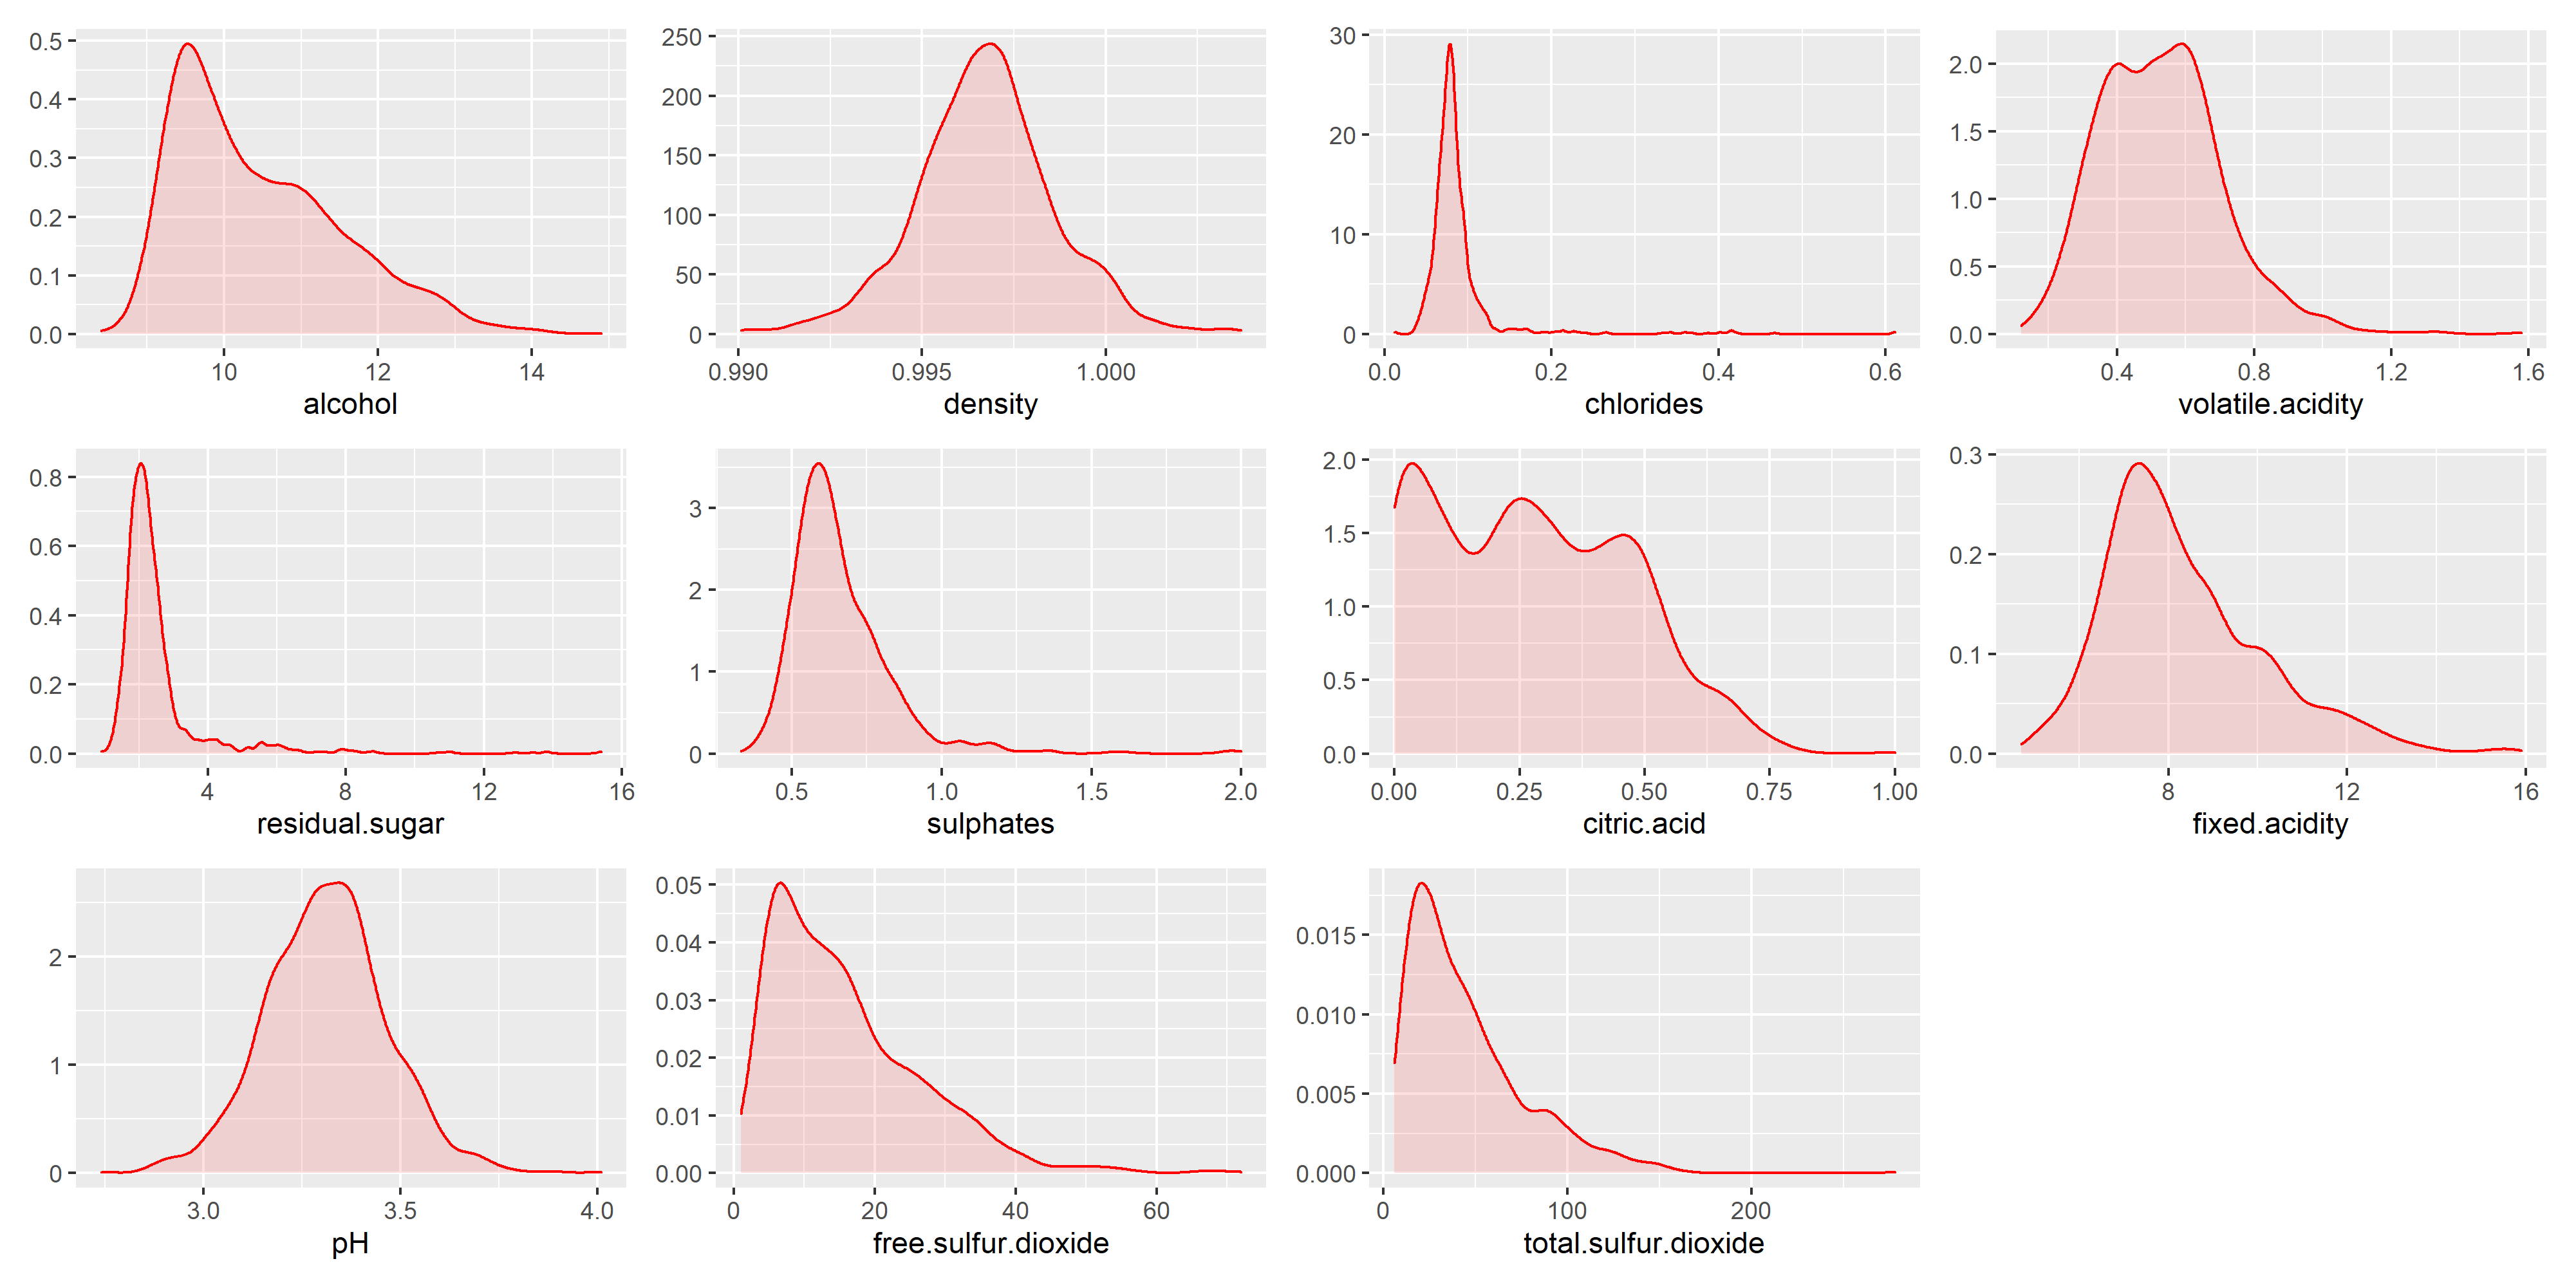
\includegraphics[width=\linewidth]{images/analisi/distribuzioni_variabili/distribution1.png}
    \caption{Questa immagine consiste in un insieme di grafici, dove ogni singolo grafico rappresenta la distribuzione dei valori assunti da una specifica variabile.}
    \label{fig:distrubution_1}
\end{figure}

\begin{figure}[H]
    \centering
    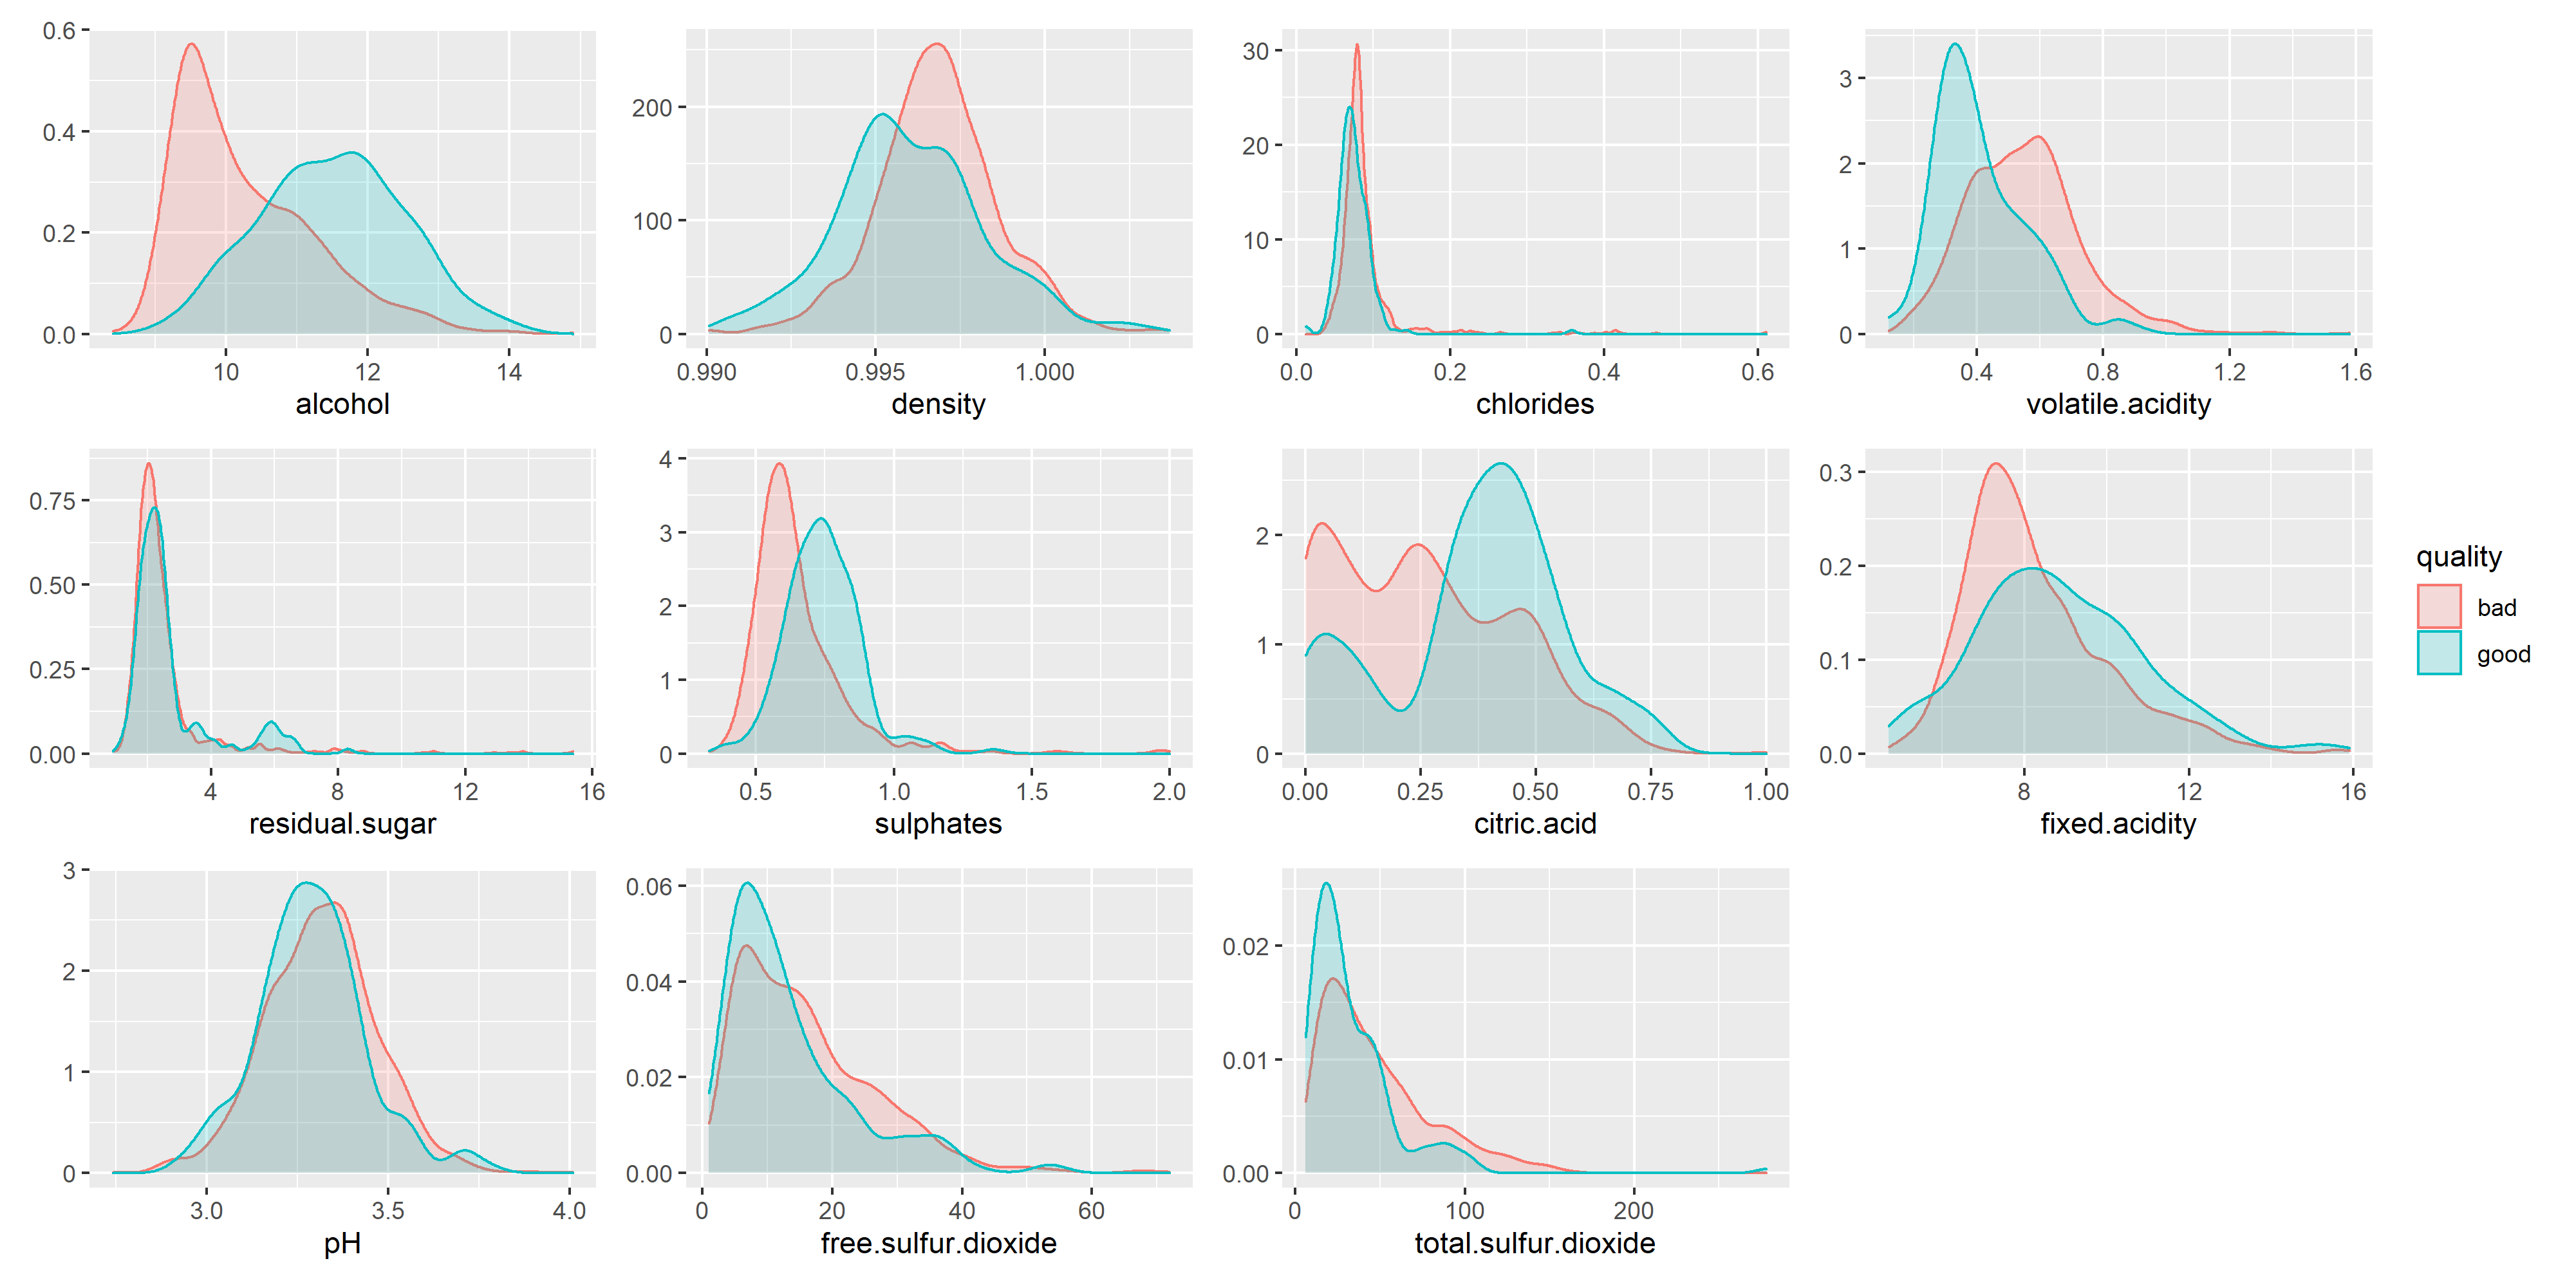
\includegraphics[width=\linewidth]{images/analisi/distribuzioni_variabili/distribution2.png}
    \caption{Questa immagine consiste in un insieme di grafici, dove ogni singolo grafico rappresenta la distribuzione dei valori assunti da una specifica variabile mettendo in evidenza la classe ($bad$ e $good$) a cui appartengono.}
    \label{fig:distrubution_2}
\end{figure}

\noindent
Dai grafici [\ref{fig:distrubution_1}] e [\ref{fig:distrubution_2}] si può notare come soltanto la variabile \textit{alcohol} abbia delle sostanziali differenze tra le due distribuzioni delle due classi e questo la rende molto interessante.

\newpage

\noindent
Le altre variabili tendono a non caratterizzare la differenza tra le due classi se non in minima parte. Questo indica la complessità presente nel distinguere le due classi per un possibile modello.

\noindent
Questa scarsa caratterizzazione rispecchia le difficoltà, già descritte nell'introduzione [\ref{ch:introduzione}], che si trovano nel produrre e nello svolgere le analisi.


\section{Analisi Outlier}
Gli outlier sono dei valori anomali o estremi, lontani dai valori centrali di un insieme di dati. Questi valori influenzano negativamente la media e la deviazione standard del dataset e quindi possono portare a risultati sbagliati. Molti algoritmi di machine learning non funzionano in modo ottimale in presenza di outlier e quindi c'è bisogno di rilevarli e rimuoverli.

\vspace{4mm}
\noindent
\`{E} stata effettuata una ricerca degli outlier su ogni attributo numerico attraverso i seguenti metodi statistici:

\subsubsection{IQR}
Gli outlier sono stati individuati usando l'approccio basato sul Interquartile Range (IQR). Lo scarto interquartile è un indice di dispersione, ovvero una misura di quanto i valori si allontanino da un valore centrale. Viene calcolato dalla differenza tra il terzo quartile (Q3) e il primo quartile (Q1). In questo approccio tutti i punti che si trovano al di sopra del valore Q3 + 1.5 * IQR o al di sotto del valore Q1 - 1.5 * IQR sono considerati outlier.

\begin{align*}
    IQR         & = Q3 - Q1        \\
    Lower Bound & = Q1 - 1.5 * IQR \\
    Upper Bound & = Q3 + 1.5 * IQR
\end{align*}

\noindent
Gli outlier possono essere rimossi o sostituiti con un valore fissato come ad esempio media, moda, mediana.
Dal momento che il dataset è sbilanciato, l'opzione di rimuovere completamente gli outlier è stata scartata perché molti di questi appartengono alla classe minoritaria.
In questo lavoro si è scelto quindi di sostituire i valori con la mediana, poiché alcune variabili hanno distribuzioni con una distorsione unilaterale e quindi corrisponde a un valore più vicino al centro rispetto alla media.

\begin{figure}
    \centering
    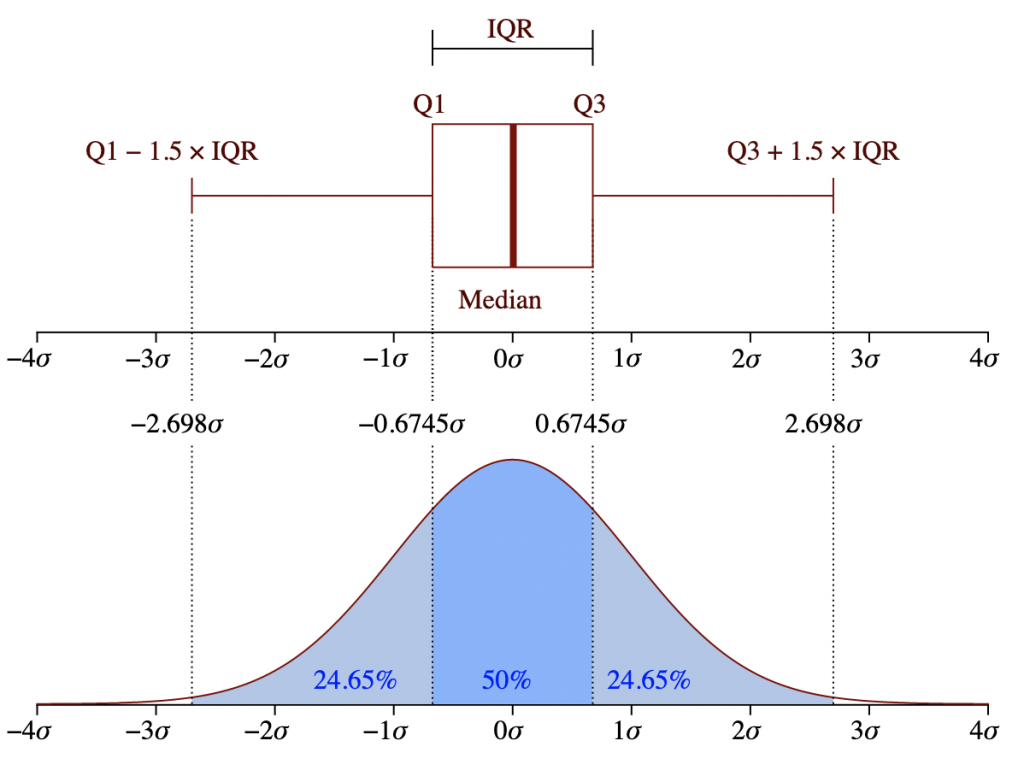
\includegraphics[width=.8\textwidth]{images/IQR.png}
    \caption{Esempio di scarto interquartile in una distribuzione normale \cite{wikipedia:iqr}}
    \label{fig:iqr}
\end{figure}

\subsubsection{Winsorizing (Percentile Capping)}
E' un metodo simile al metodo IQR, in questo caso si utilizzano due percentili. Tutti i valori sotto al minimo valore dell'intervallo vengono sostituiti con il minimo, e tutti i valori sopra il massimo valore dell'intervallo vengono sostituiti con il massimo. In questo lavoro sono stati usati due intervalli ($5^{\circ}$ percentile, $95^{\circ}$ percentile) e ($1^{\circ}$ percentile, $99^{\circ}$ percentile).

\noindent
I due intervalli sono stati denominati Winsorizing 90\% e Winsorizing 98\%:
\begin{itemize}
    \item Winsorizing 90\% indica che il 5\% inferiore dei dati viene sostituito con il $5^{\circ}$ percentile e il 5\% superiore dei dati viene sostituito con il $95^{\circ}$ percentile.
    \item Winsorizing 98\% indica che l' 1\% inferiore dei dati viene sostituito con il $1^{\circ}$ percentile e l' 1\% superiore dei dati viene sostituito con il $99^{\circ}$ percentile.
\end{itemize}

\subsubsection{Metodo Scelto}
Un grafico abbastanza semplice e veloce per visualizzare gli outlier è il boxplot. \'{E} stato confrontato ogni variabile del dataset con i valori assunti dopo l'applicazione dei metodi di rimozione degli outlier (IQR, Winsorizing 90\% e Winsorizing 98\%), attraverso dei boxplot. Sopra a ogni boxplot sono stati riportati i valori divisi per qualità.

\noindent
Il metodo Winsorizing rileva un intervallo di outlier più piccolo e variabile rispetto all'IQR. Inoltre nei casi di distribuzione con distorsione laterale accumula troppi valori agli estremi, alterando così la distribuzione. Con il metodo Winsorizing 98\% si risulta avere una distribuzione più smussata agli estremi. Il metodo IQR, sostituendo con la mediana non altera molto la distribuzione.
Per decidere il metodo più efficace da usare sono stati confrontati dati dopo l'applicazione di ogni metodo attraverso dei Q-Q plot.

\noindent
I Q-Q (quantile-quantile) plot sono dei grafici utili per capire se due insiemi di dati hanno la stessa distribuzione. Vengono rappresentati i punti in un piano cartesiano attraverso una coppia di quantili. Inoltre viene tracciata una retta a 45° in modo da evidenziare i punti più vicini alla retta. Due insiemi di dati hanno una distribuzione simile se i punti cadono approssimatamene sulla linea di riferimento.
Analizzando i grafici si è visto che il metodo IQR ha valori più vicini alla retta, quindi si è scelto di utilizzare questo.

\noindent
Nelle seguenti tabelle sono stati riportati le varie statistiche descrittive delle variabili prima e dopo la rimozione degli outlier con il metodo scelto.

\begin{table}[H]
\centering
\resizebox{\linewidth}{!}{
\begin{tabular}[t]{lrrrrrrrr}
\toprule
  & vars & mean & sd & median & min & max & skew & kurtosis\\
\midrule
\cellcolor{gray!6}{fixed.acidity} & \cellcolor{gray!6}{1} & \cellcolor{gray!6}{8.34} & \cellcolor{gray!6}{1.78} & \cellcolor{gray!6}{7.90} & \cellcolor{gray!6}{4.70} & \cellcolor{gray!6}{15.90} & \cellcolor{gray!6}{0.98} & \cellcolor{gray!6}{1.13}\\
volatile.acidity & 2 & 0.53 & 0.18 & 0.52 & 0.12 & 1.58 & 0.71 & 1.46\\
\cellcolor{gray!6}{citric.acid} & \cellcolor{gray!6}{3} & \cellcolor{gray!6}{0.27} & \cellcolor{gray!6}{0.19} & \cellcolor{gray!6}{0.26} & \cellcolor{gray!6}{0.00} & \cellcolor{gray!6}{1.00} & \cellcolor{gray!6}{0.32} & \cellcolor{gray!6}{-0.79}\\
residual.sugar & 4 & 2.53 & 1.40 & 2.20 & 0.90 & 15.40 & 4.47 & 27.53\\
\cellcolor{gray!6}{chlorides} & \cellcolor{gray!6}{5} & \cellcolor{gray!6}{0.09} & \cellcolor{gray!6}{0.05} & \cellcolor{gray!6}{0.08} & \cellcolor{gray!6}{0.01} & \cellcolor{gray!6}{0.61} & \cellcolor{gray!6}{5.89} & \cellcolor{gray!6}{45.36}\\
\addlinespace
free.sulfur.dioxide & 6 & 15.79 & 10.58 & 13.00 & 1.00 & 72.00 & 1.29 & 2.19\\
\cellcolor{gray!6}{total.sulfur.dioxide} & \cellcolor{gray!6}{7} & \cellcolor{gray!6}{45.23} & \cellcolor{gray!6}{31.87} & \cellcolor{gray!6}{37.00} & \cellcolor{gray!6}{6.00} & \cellcolor{gray!6}{278.00} & \cellcolor{gray!6}{1.41} & \cellcolor{gray!6}{2.87}\\
density & 8 & 1.00 & 0.00 & 1.00 & 0.99 & 1.00 & 0.05 & 0.90\\
\cellcolor{gray!6}{pH} & \cellcolor{gray!6}{9} & \cellcolor{gray!6}{3.31} & \cellcolor{gray!6}{0.15} & \cellcolor{gray!6}{3.31} & \cellcolor{gray!6}{2.74} & \cellcolor{gray!6}{4.01} & \cellcolor{gray!6}{0.11} & \cellcolor{gray!6}{0.62}\\
sulphates & 10 & 0.66 & 0.17 & 0.62 & 0.33 & 2.00 & 2.57 & 13.02\\
\addlinespace
\cellcolor{gray!6}{alcohol} & \cellcolor{gray!6}{11} & \cellcolor{gray!6}{10.45} & \cellcolor{gray!6}{1.07} & \cellcolor{gray!6}{10.20} & \cellcolor{gray!6}{8.40} & \cellcolor{gray!6}{14.90} & \cellcolor{gray!6}{0.84} & \cellcolor{gray!6}{0.13}\\
\bottomrule
\end{tabular}}
\caption{Prima della rimozione}
\end{table}


\begin{table}
\centering
\resizebox{\linewidth}{!}{
\begin{tabular}[t]{lrrrrrrrr}
\toprule
  & vars & mean & sd & median & min & max & skew & kurtosis\\
\midrule
\cellcolor{gray!6}{fixed.acidity} & \cellcolor{gray!6}{1} & \cellcolor{gray!6}{6.83} & \cellcolor{gray!6}{0.77} & \cellcolor{gray!6}{6.80} & \cellcolor{gray!6}{4.70} & \cellcolor{gray!6}{9.00} & \cellcolor{gray!6}{0.22} & \cellcolor{gray!6}{0.02}\\
volatile.acidity & 2 & 0.27 & 0.08 & 0.26 & 0.08 & 0.48 & 0.41 & -0.23\\
\cellcolor{gray!6}{citric.acid} & \cellcolor{gray!6}{3} & \cellcolor{gray!6}{0.32} & \cellcolor{gray!6}{0.09} & \cellcolor{gray!6}{0.31} & \cellcolor{gray!6}{0.10} & \cellcolor{gray!6}{0.57} & \cellcolor{gray!6}{0.41} & \cellcolor{gray!6}{-0.02}\\
residual.sugar & 4 & 6.39 & 4.96 & 5.20 & 0.60 & 22.00 & 0.73 & -0.52\\
\cellcolor{gray!6}{chlorides} & \cellcolor{gray!6}{5} & \cellcolor{gray!6}{0.04} & \cellcolor{gray!6}{0.01} & \cellcolor{gray!6}{0.04} & \cellcolor{gray!6}{0.02} & \cellcolor{gray!6}{0.07} & \cellcolor{gray!6}{0.10} & \cellcolor{gray!6}{-0.25}\\
\addlinespace
free.sulfur.dioxide & 6 & 34.53 & 15.28 & 33.00 & 2.00 & 78.00 & 0.32 & -0.45\\
\cellcolor{gray!6}{total.sulfur.dioxide} & \cellcolor{gray!6}{7} & \cellcolor{gray!6}{138.24} & \cellcolor{gray!6}{41.26} & \cellcolor{gray!6}{135.00} & \cellcolor{gray!6}{21.00} & \cellcolor{gray!6}{256.00} & \cellcolor{gray!6}{0.23} & \cellcolor{gray!6}{-0.33}\\
density & 8 & 0.99 & 0.00 & 0.99 & 0.99 & 1.00 & 0.23 & -0.78\\
\cellcolor{gray!6}{pH} & \cellcolor{gray!6}{9} & \cellcolor{gray!6}{3.18} & \cellcolor{gray!6}{0.14} & \cellcolor{gray!6}{3.17} & \cellcolor{gray!6}{2.79} & \cellcolor{gray!6}{3.57} & \cellcolor{gray!6}{0.22} & \cellcolor{gray!6}{-0.18}\\
sulphates & 10 & 0.48 & 0.10 & 0.47 & 0.23 & 0.76 & 0.48 & -0.08\\
\addlinespace
\cellcolor{gray!6}{alcohol} & \cellcolor{gray!6}{11} & \cellcolor{gray!6}{10.52} & \cellcolor{gray!6}{1.24} & \cellcolor{gray!6}{10.40} & \cellcolor{gray!6}{8.00} & \cellcolor{gray!6}{14.20} & \cellcolor{gray!6}{0.49} & \cellcolor{gray!6}{-0.69}\\
\bottomrule
\end{tabular}}
\end{table}


\subsection{Grafici}

\begin{figure}[H]
    \centering

    \subfloat[]{%
        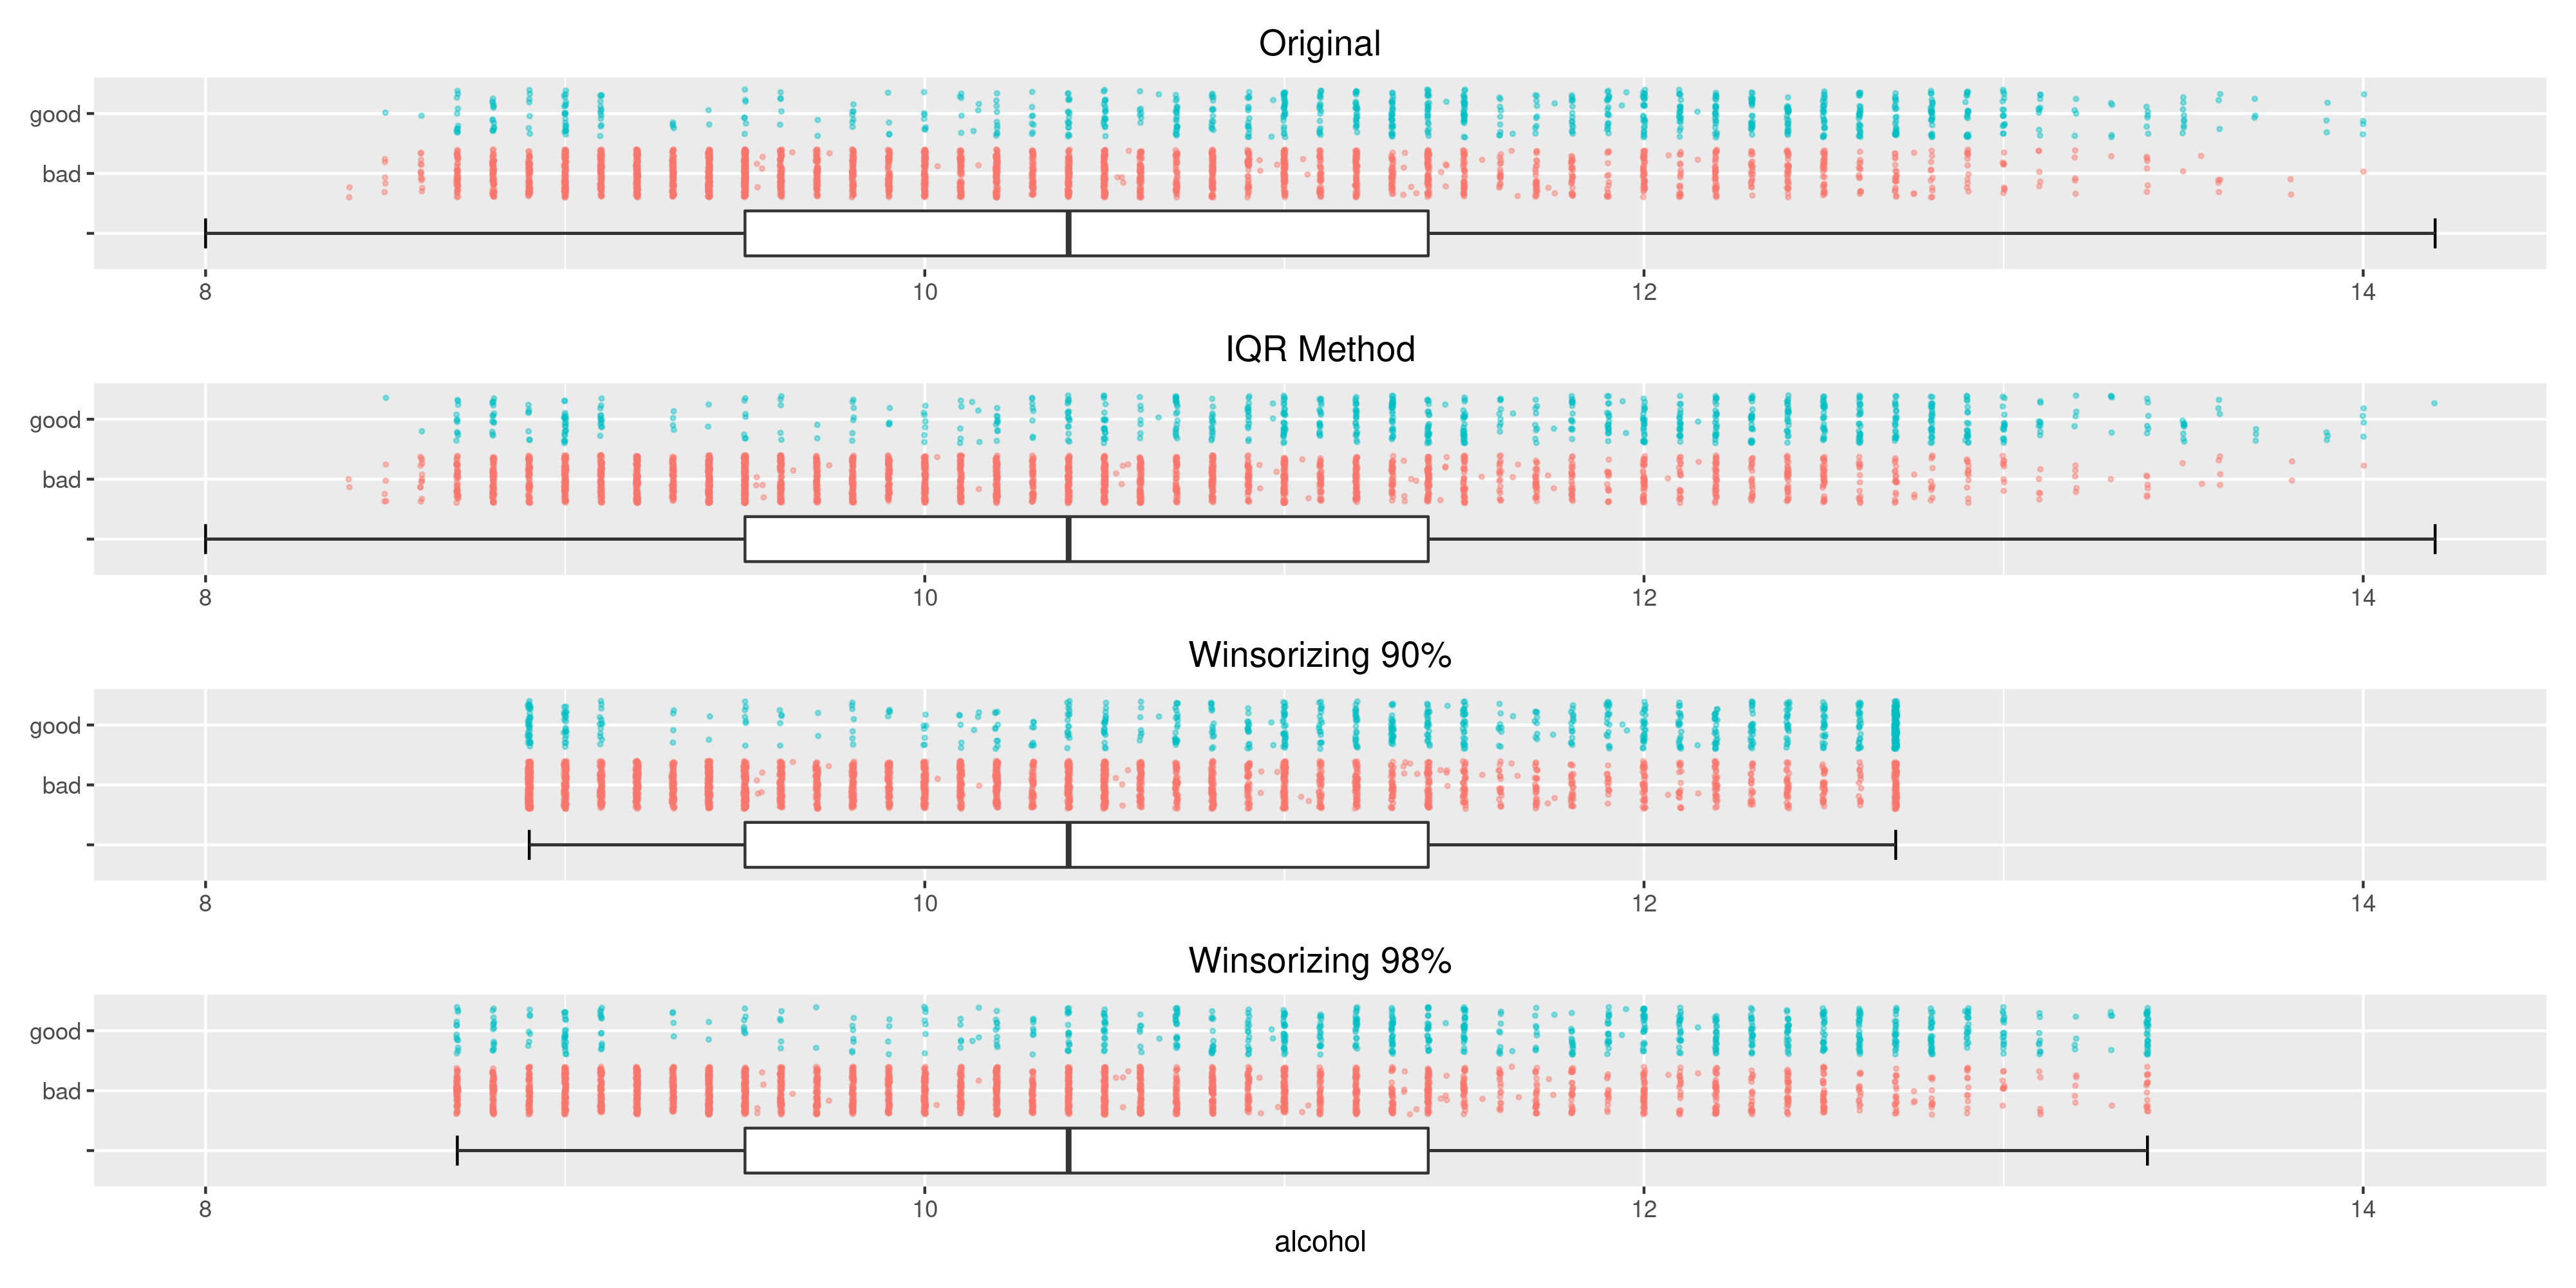
\includegraphics[width=0.99\textwidth]{images/outliers/alcohol_boxplot.png}
    }

    \subfloat[]{%
        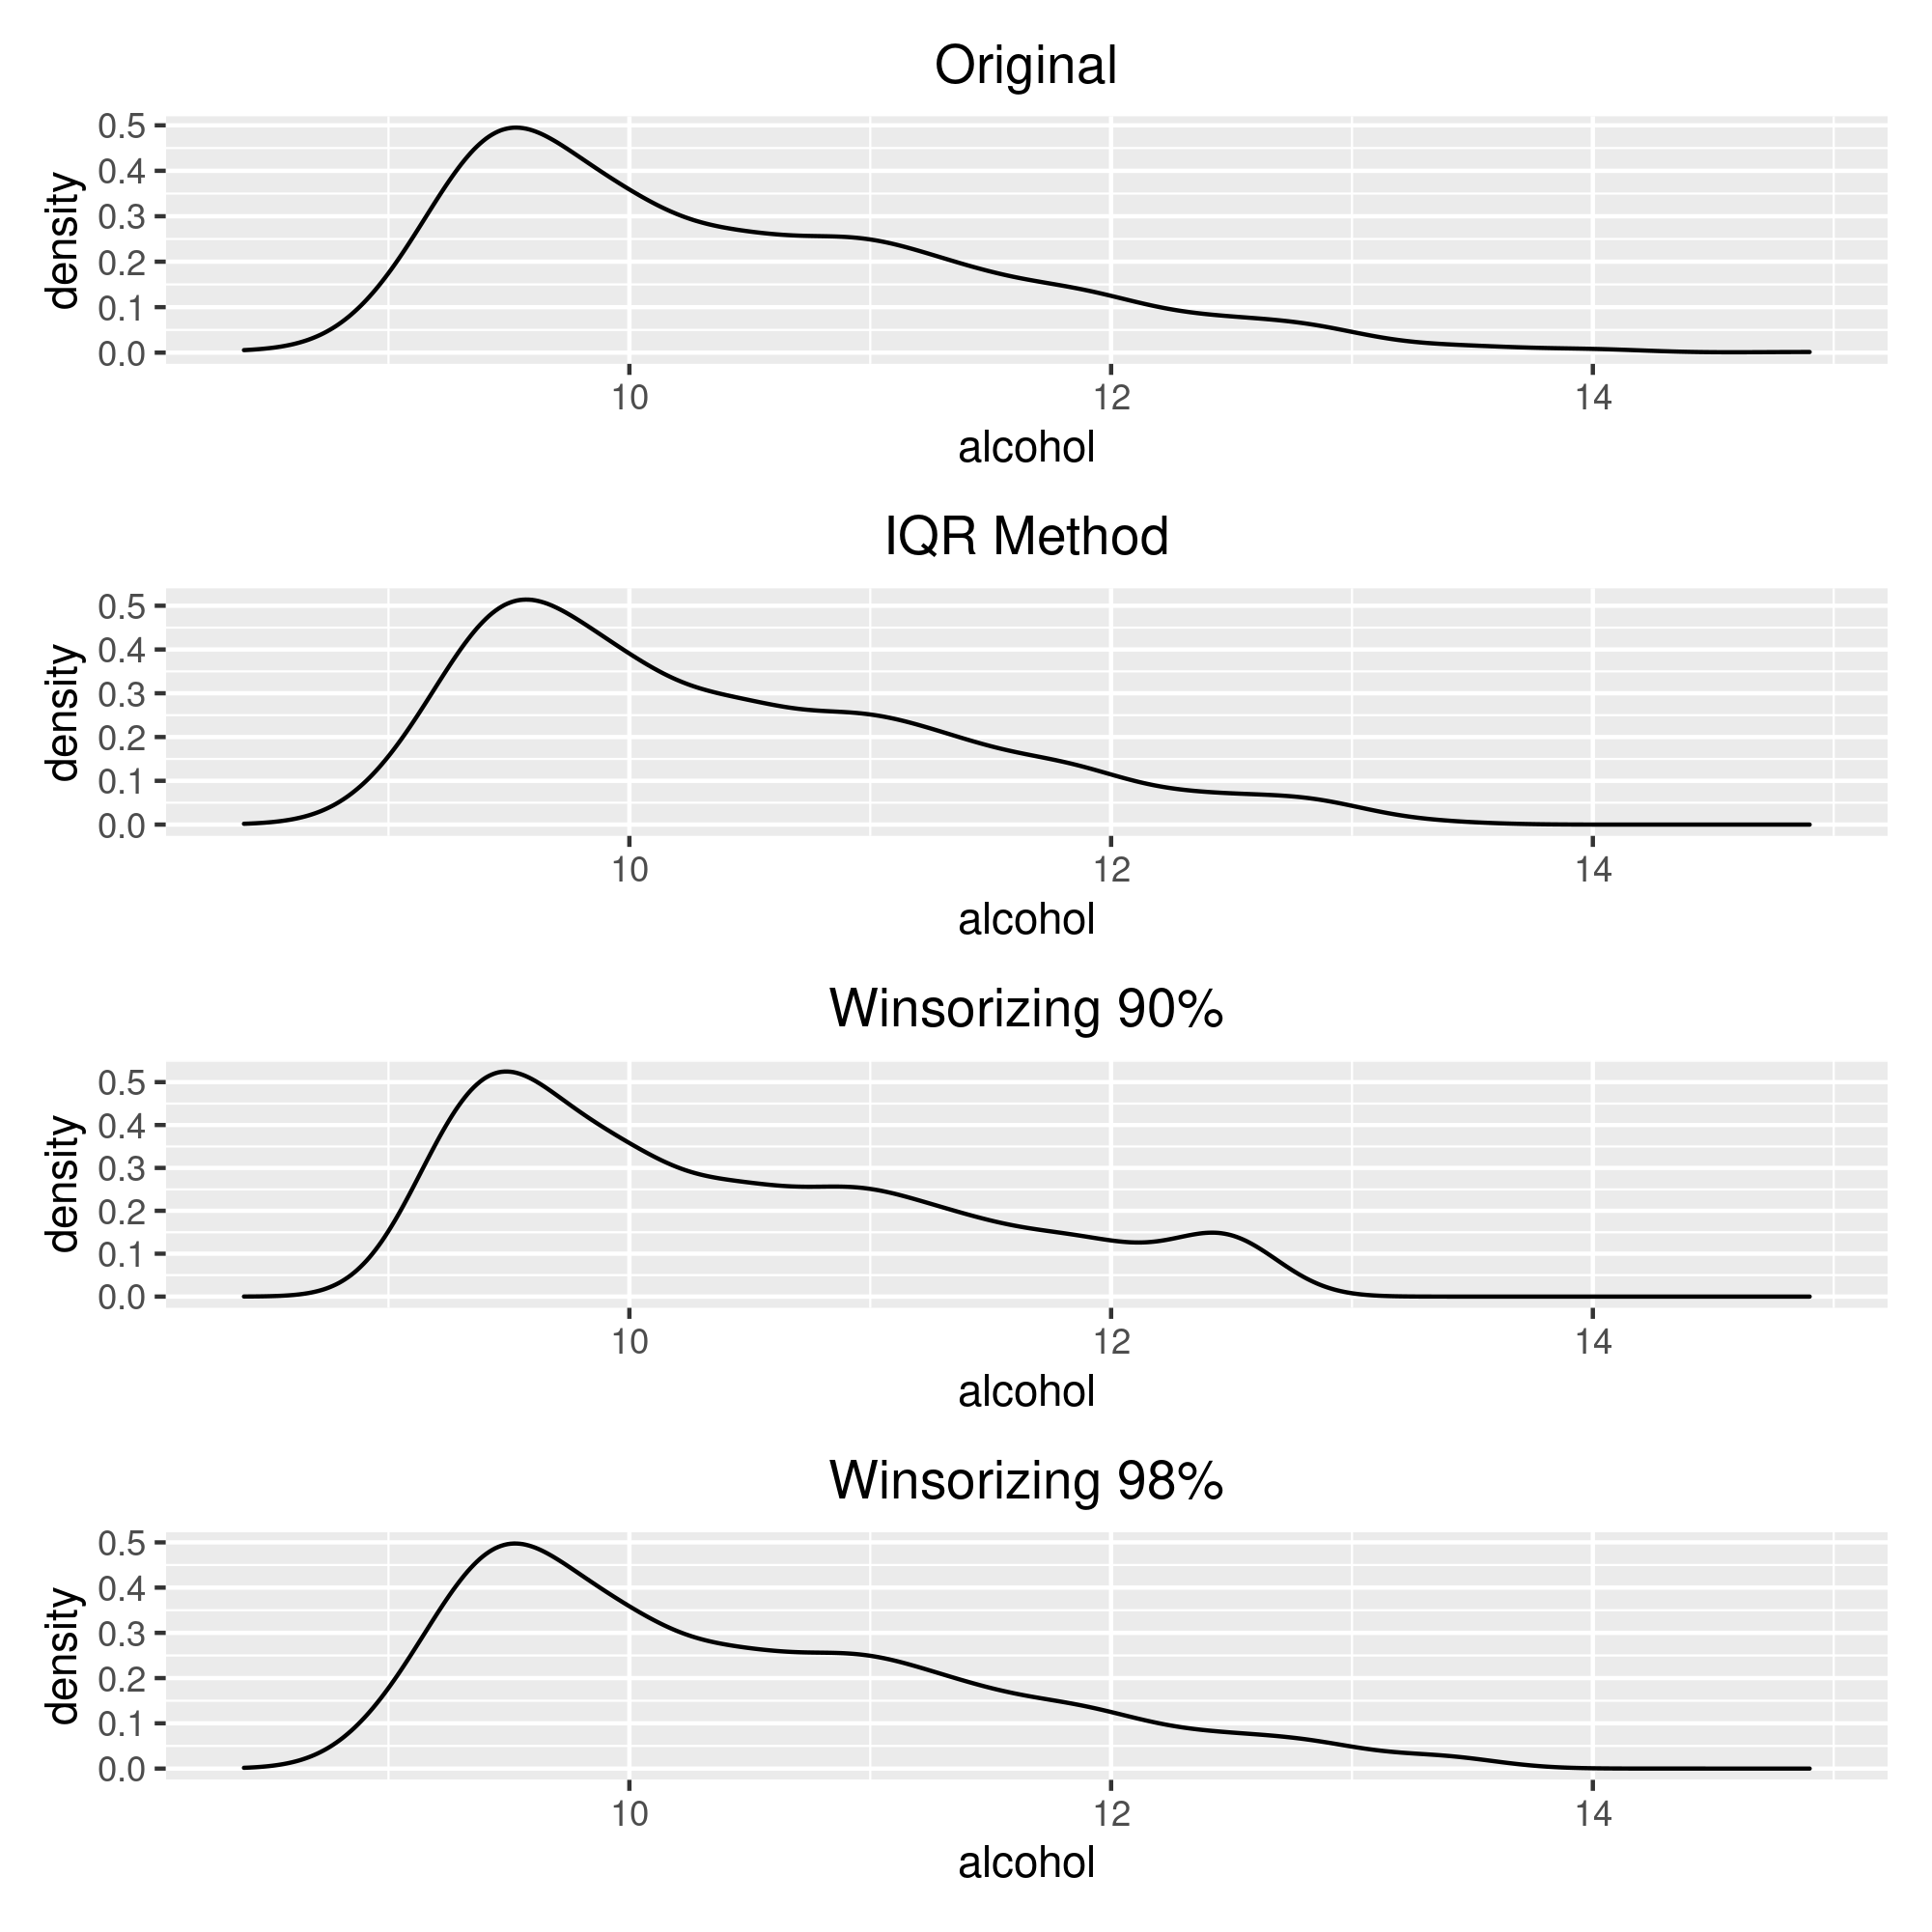
\includegraphics[width=0.45\textwidth]{images/outliers/alcohol_distribution.png}
    }\qquad
    \subfloat[]{%
        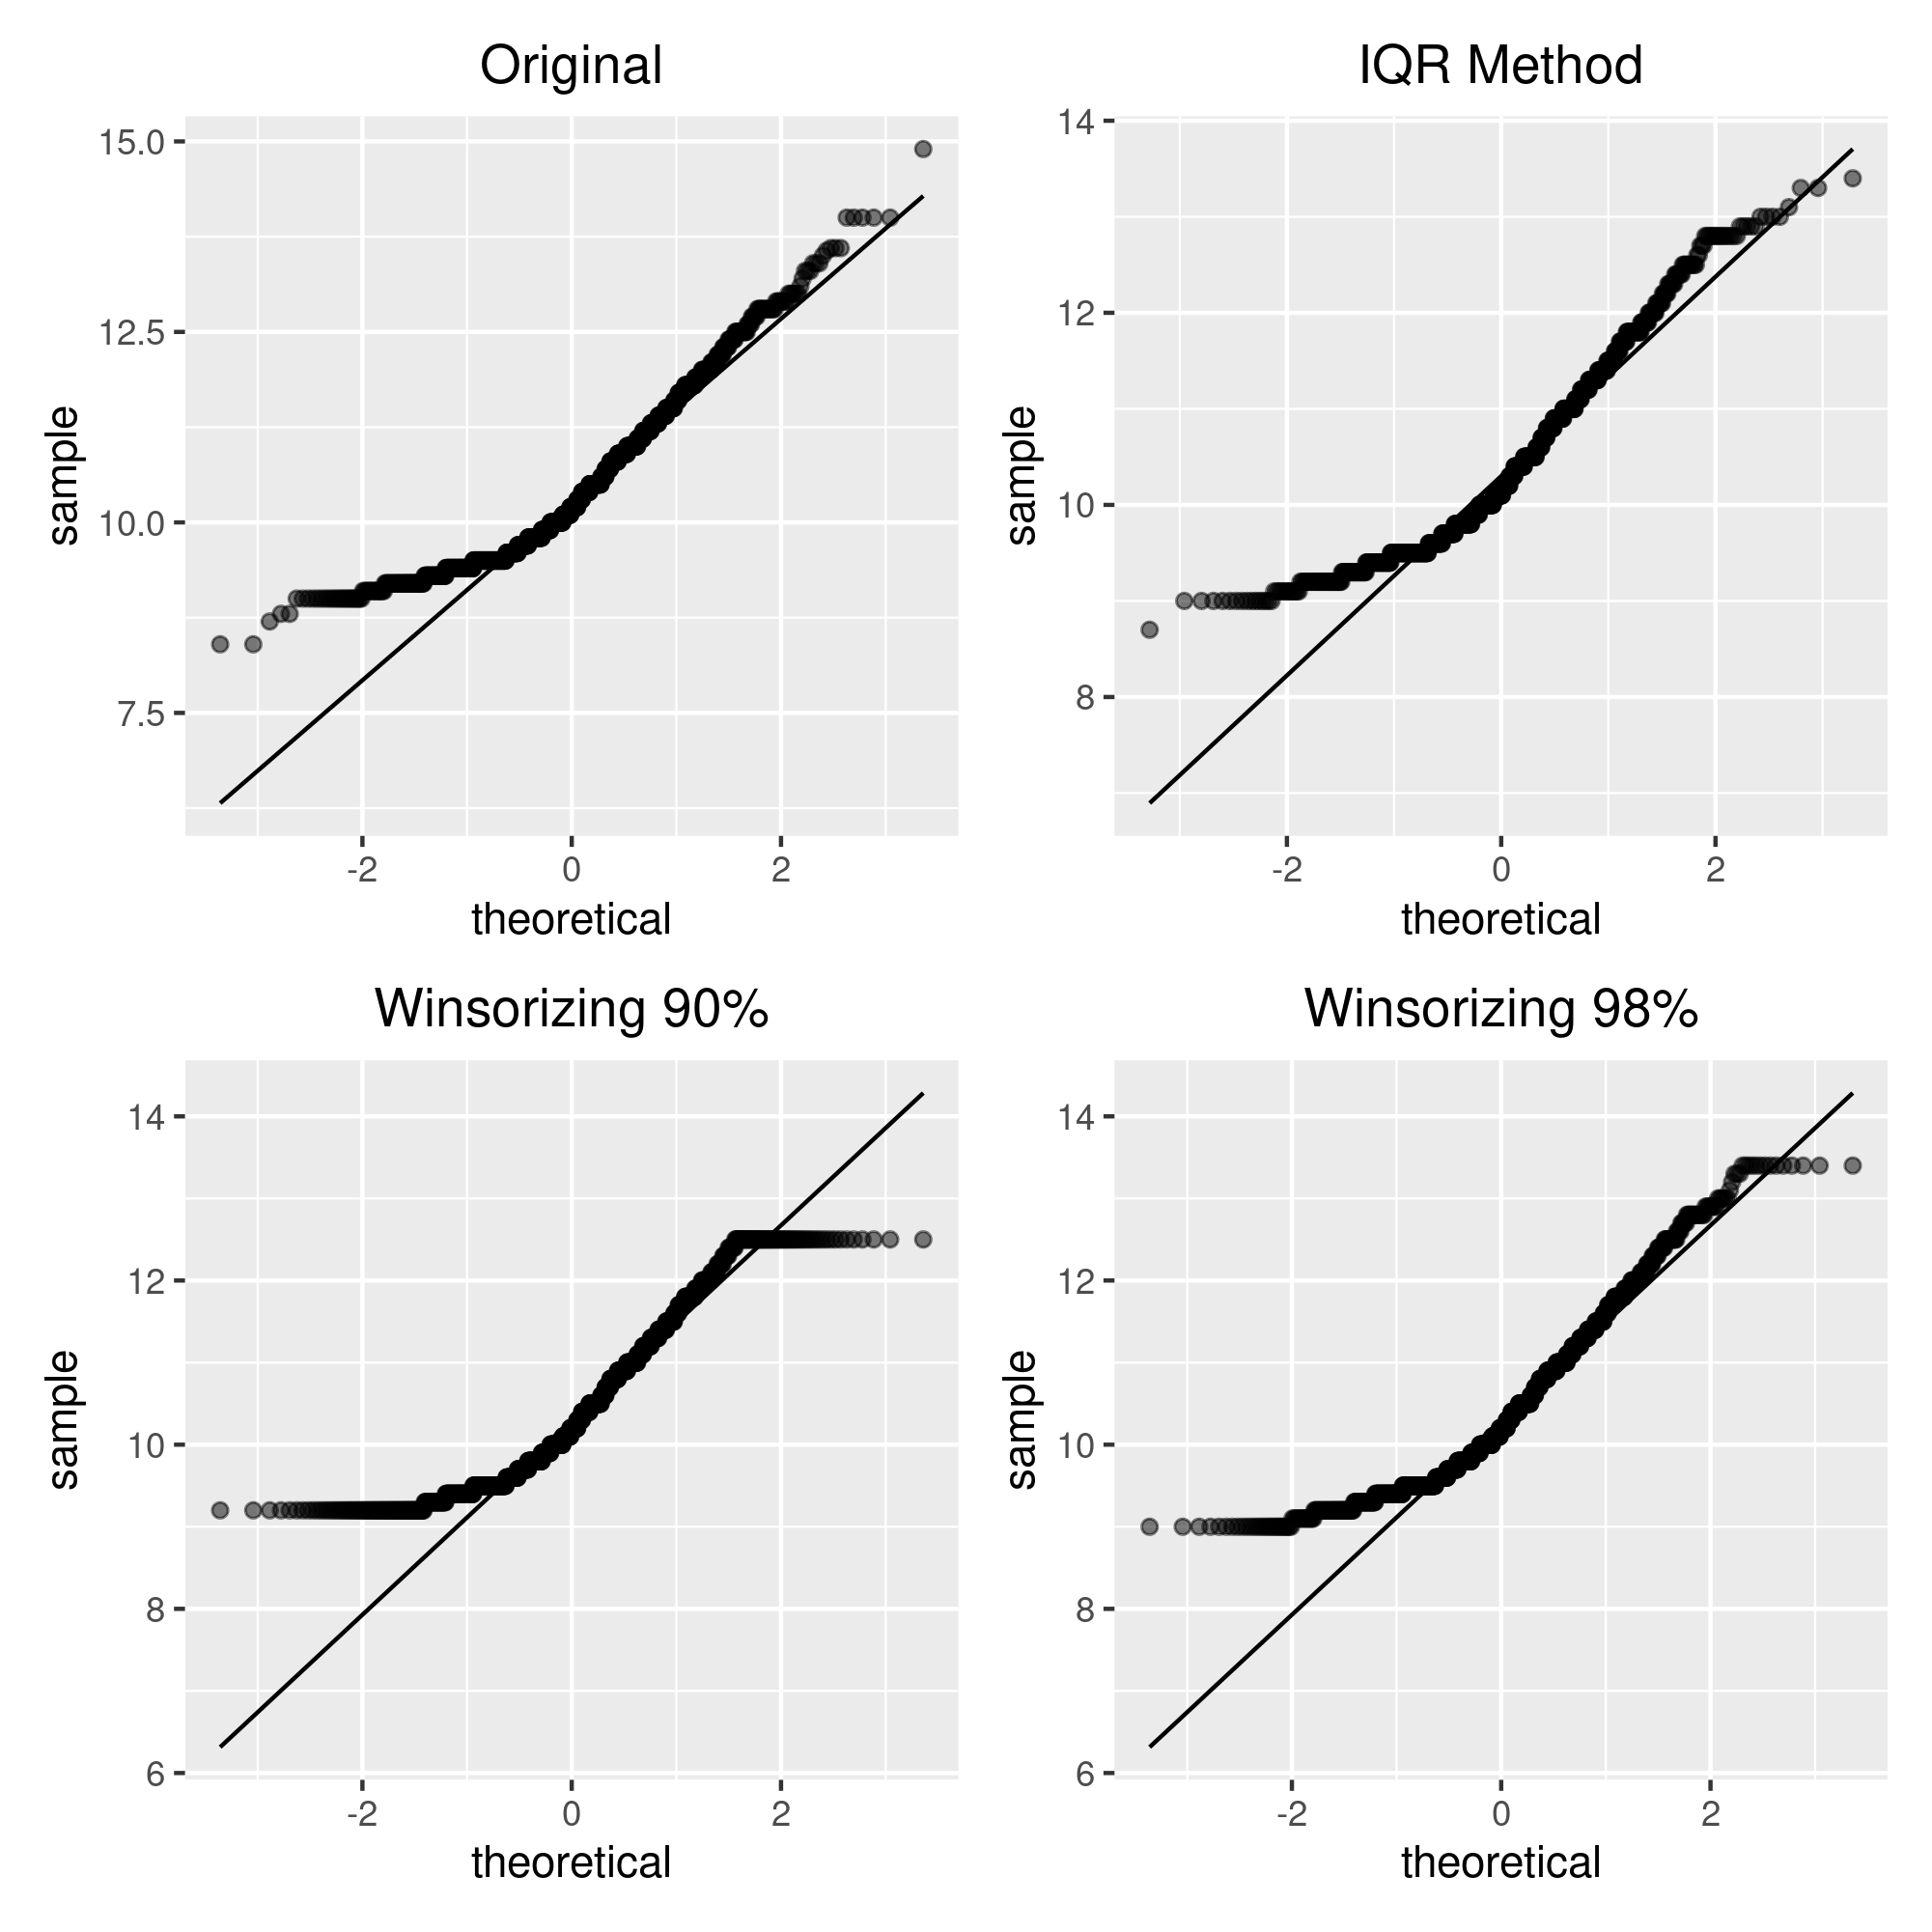
\includegraphics[width=0.45\textwidth]{images/outliers/alcohol_qqplot.png}
    }

    \label{fig:alcohol}
    \caption{Commento}
\end{figure}

\begin{figure}[H]
    \centering

    \subfloat[]{%
        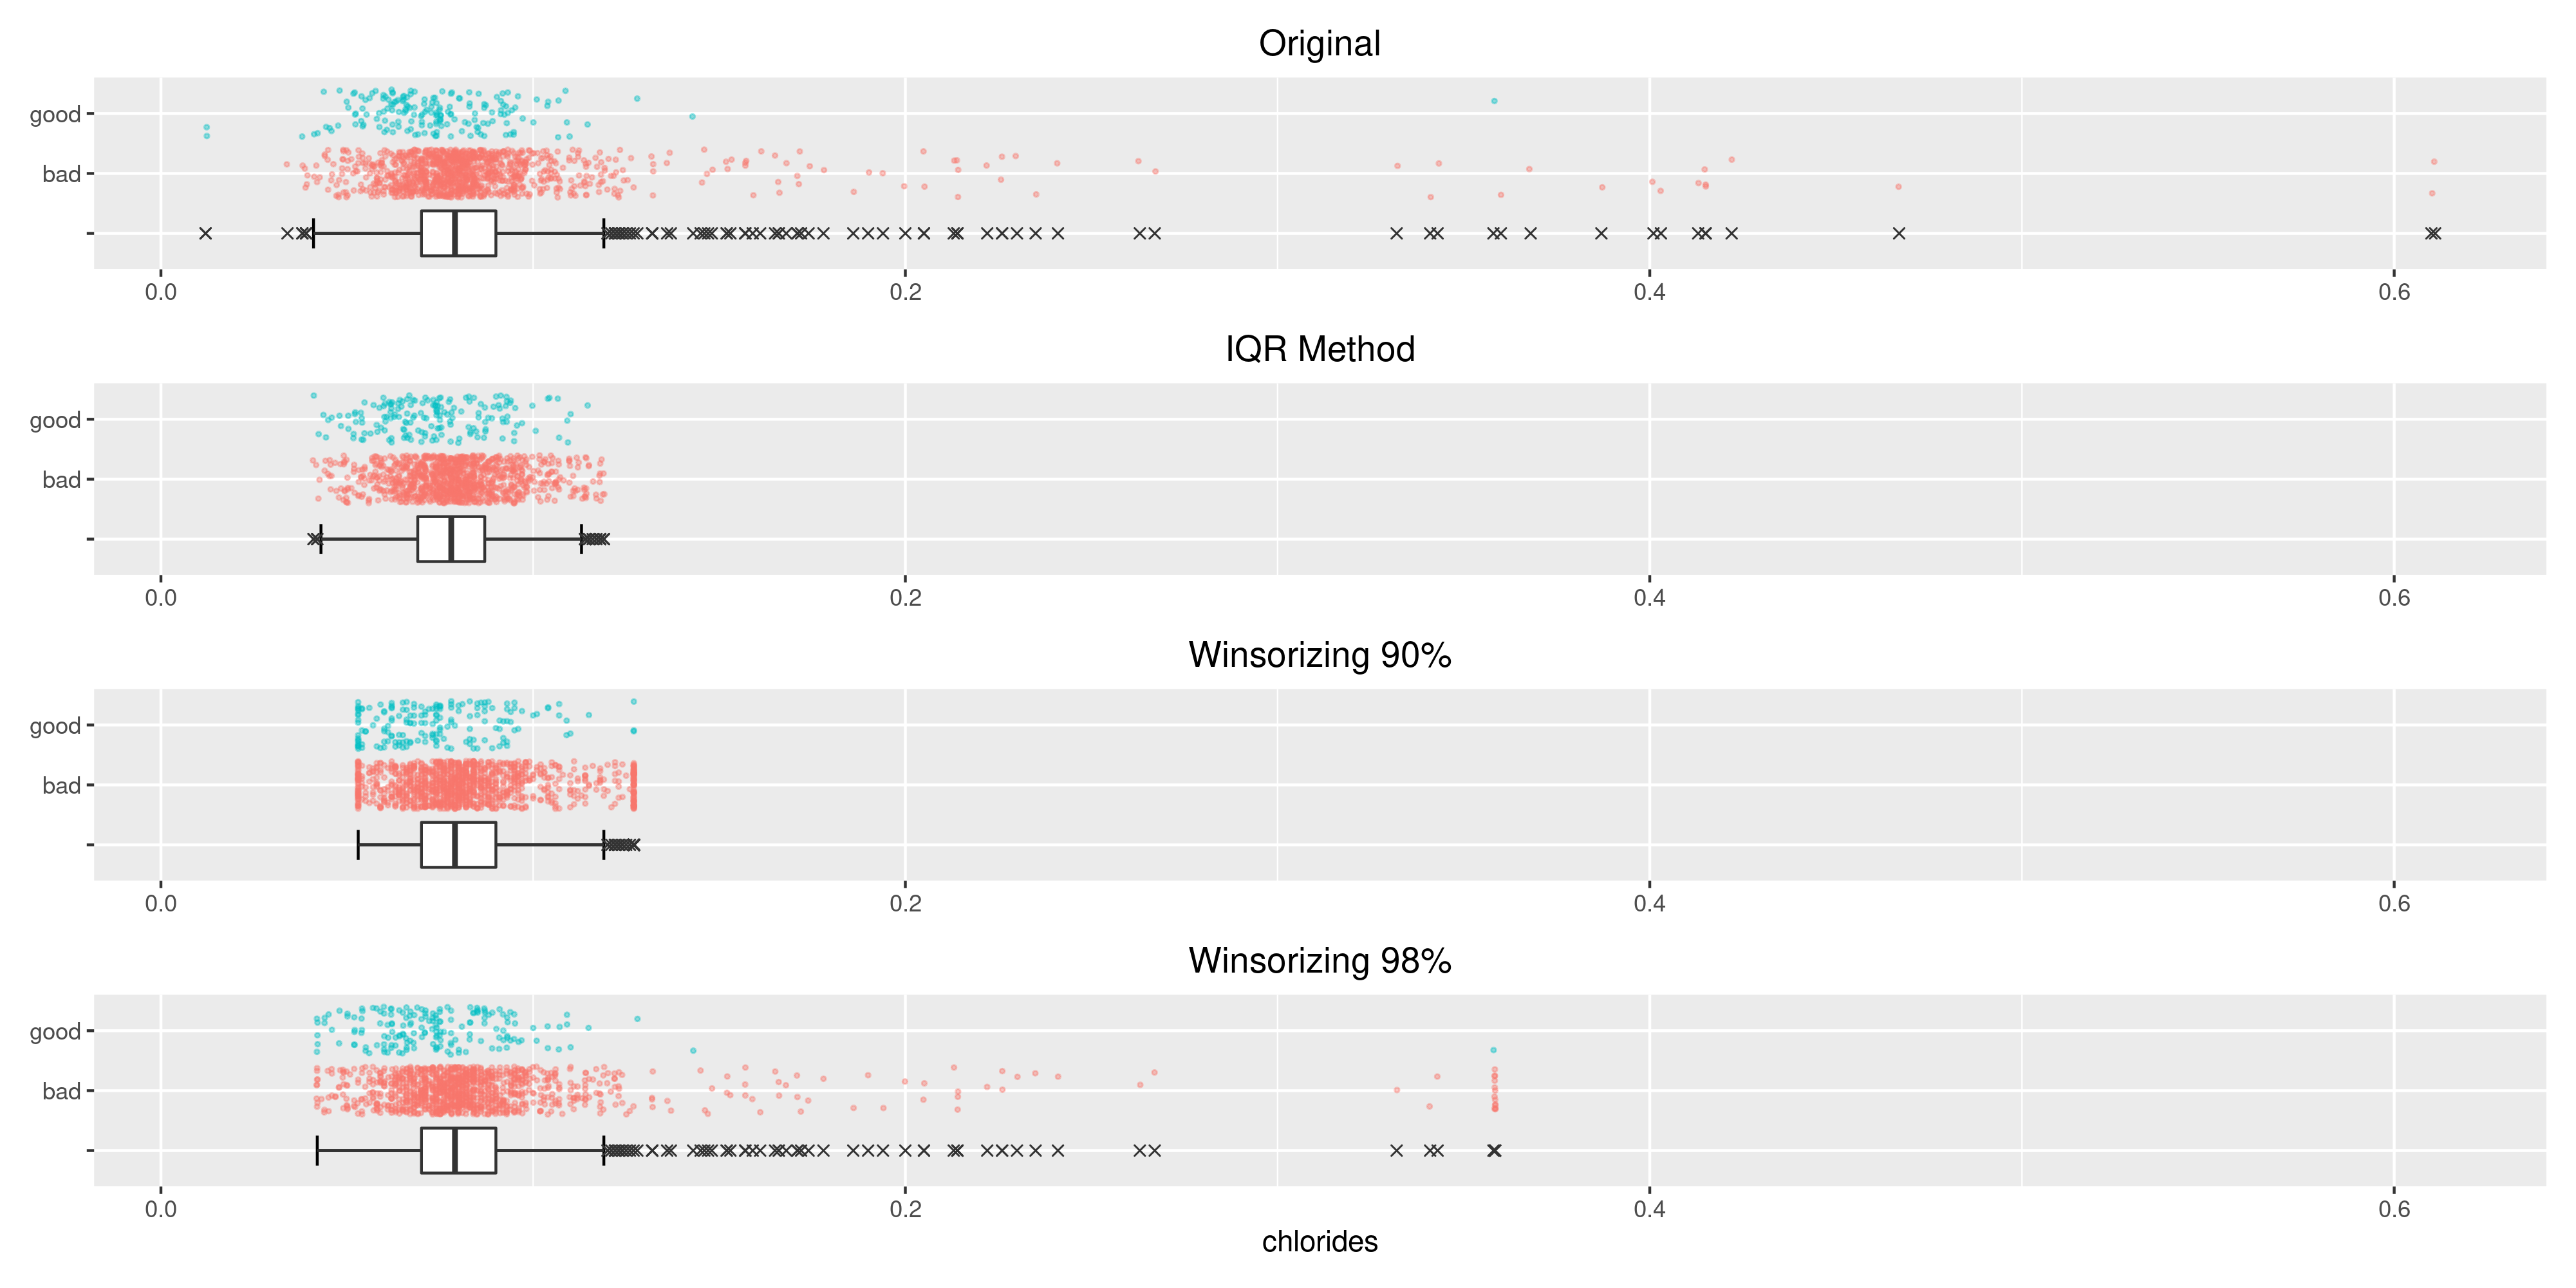
\includegraphics[width=0.99\textwidth]{images/outliers/chlorides_boxplot.png}
    }

    \subfloat[]{%
        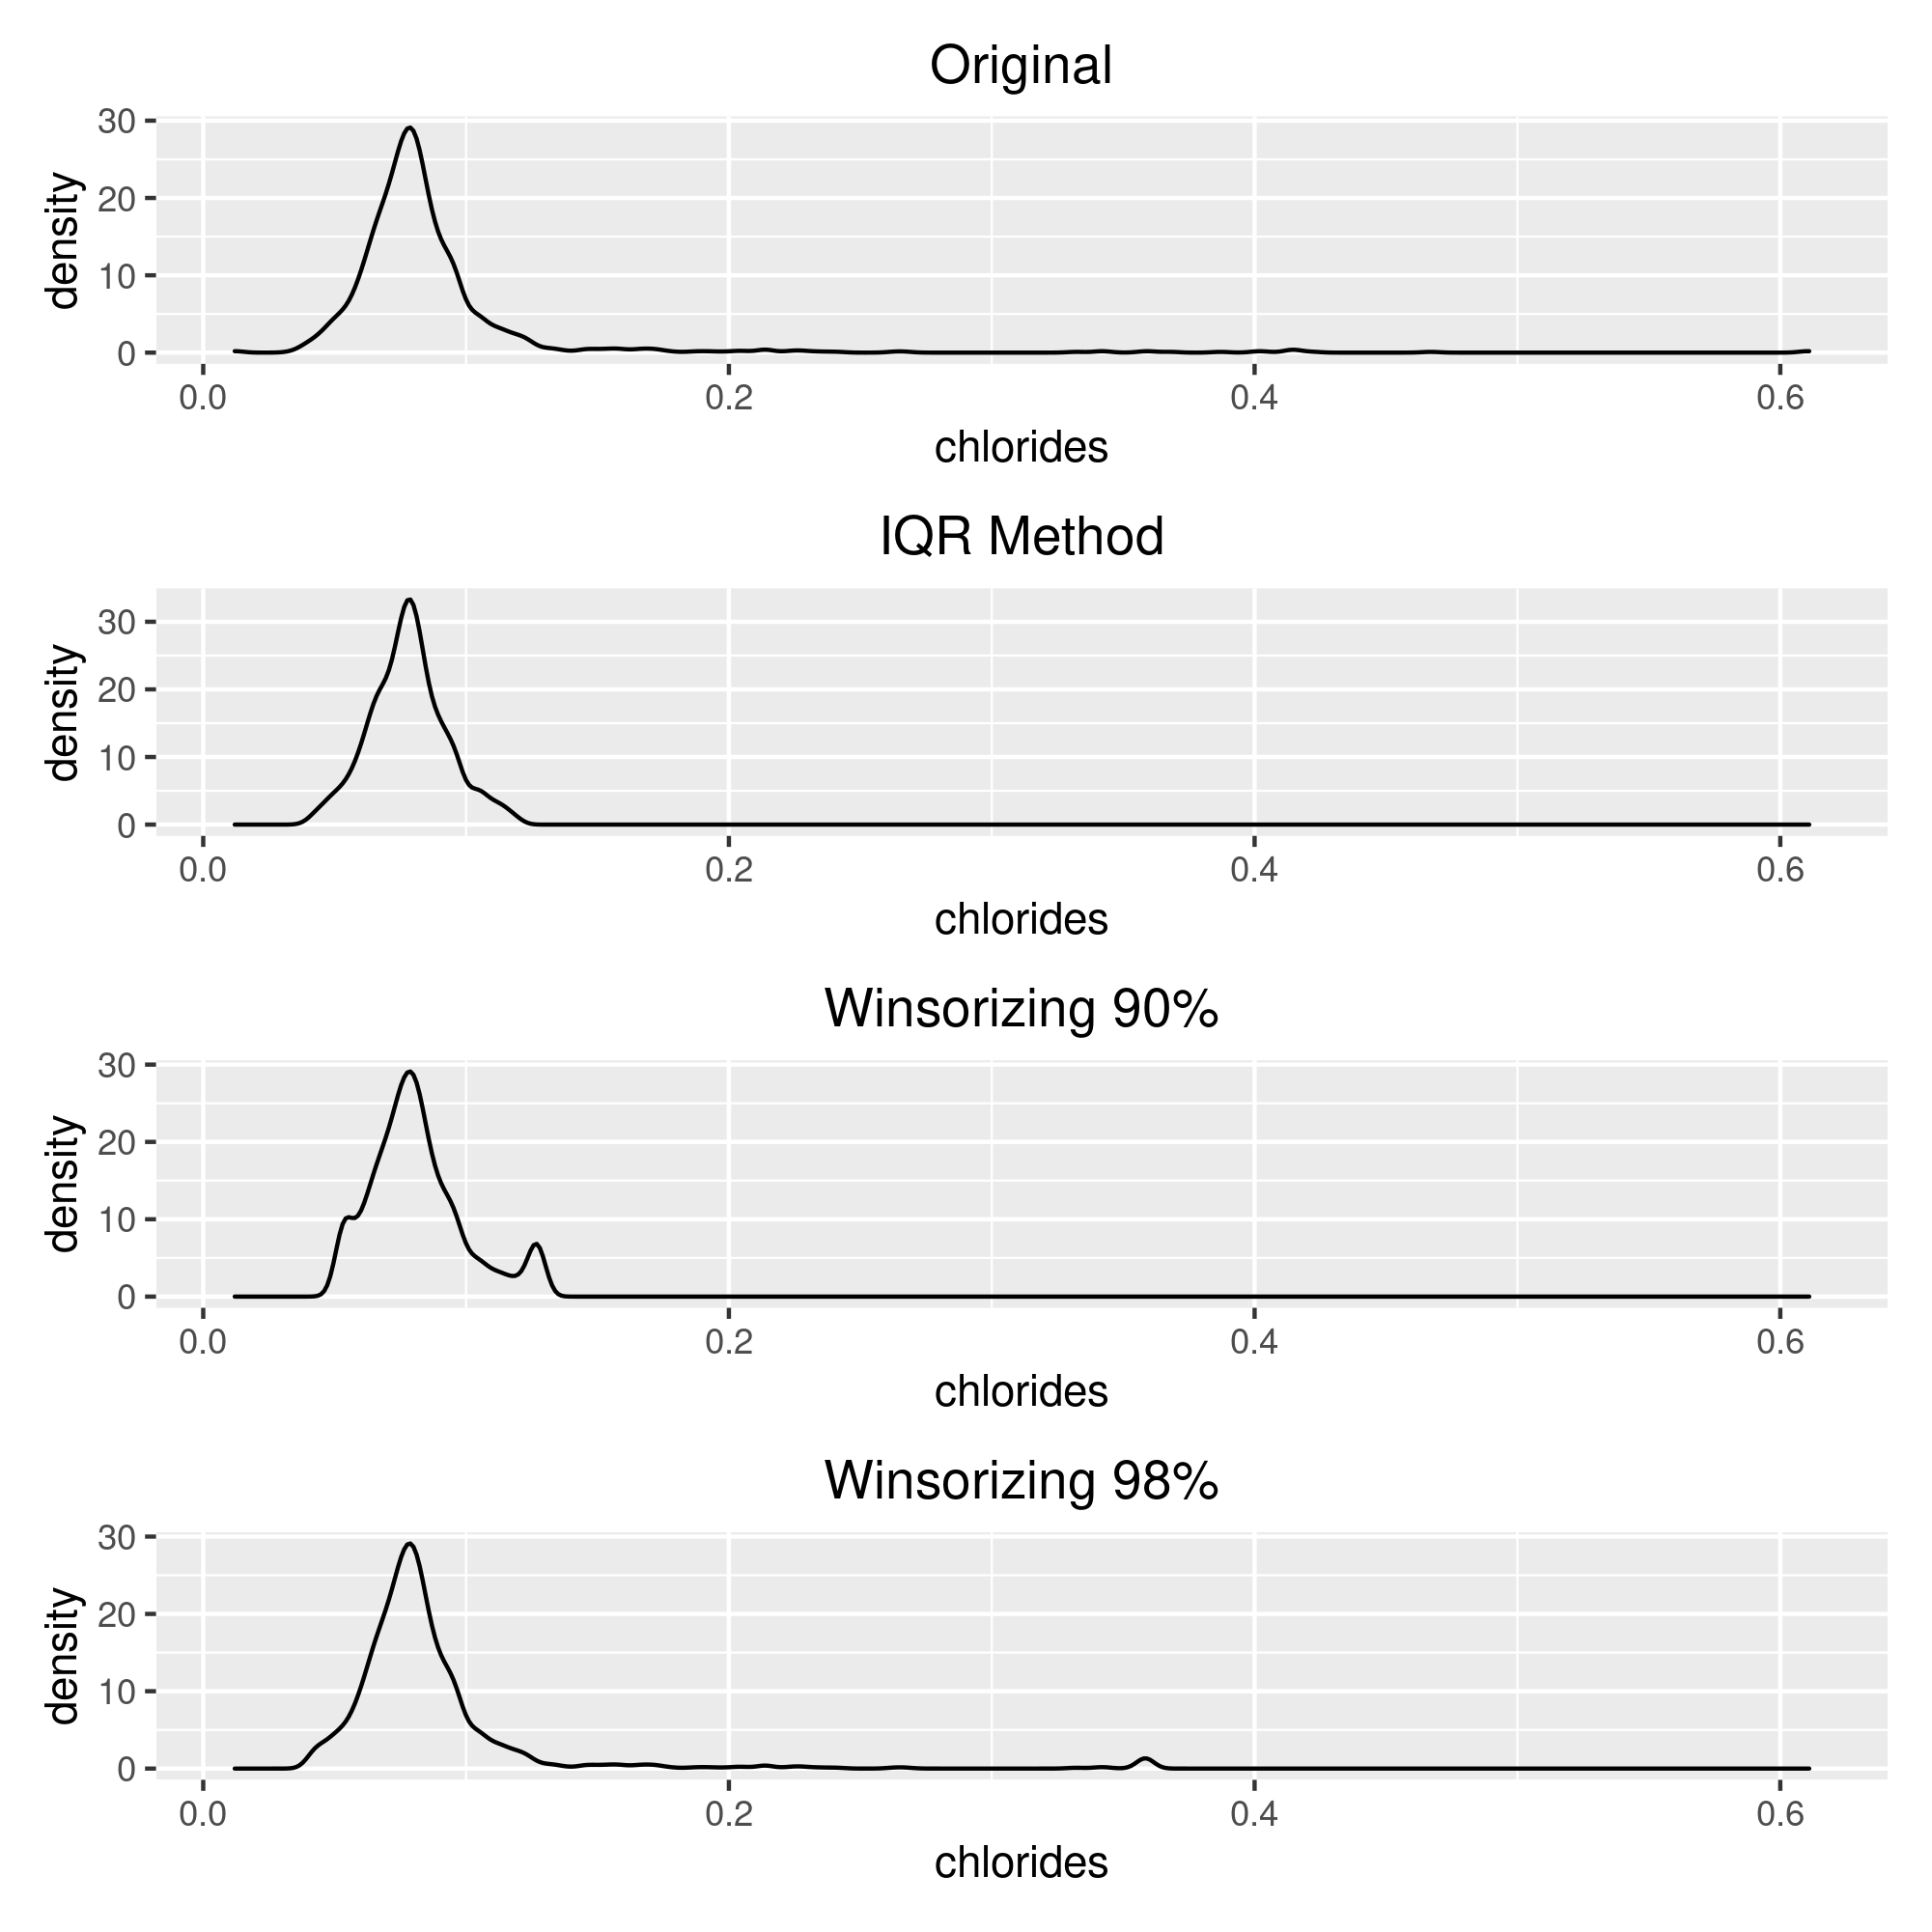
\includegraphics[width=0.45\textwidth]{images/outliers/chlorides_distribution.png}
    }\qquad
    \subfloat[]{%
        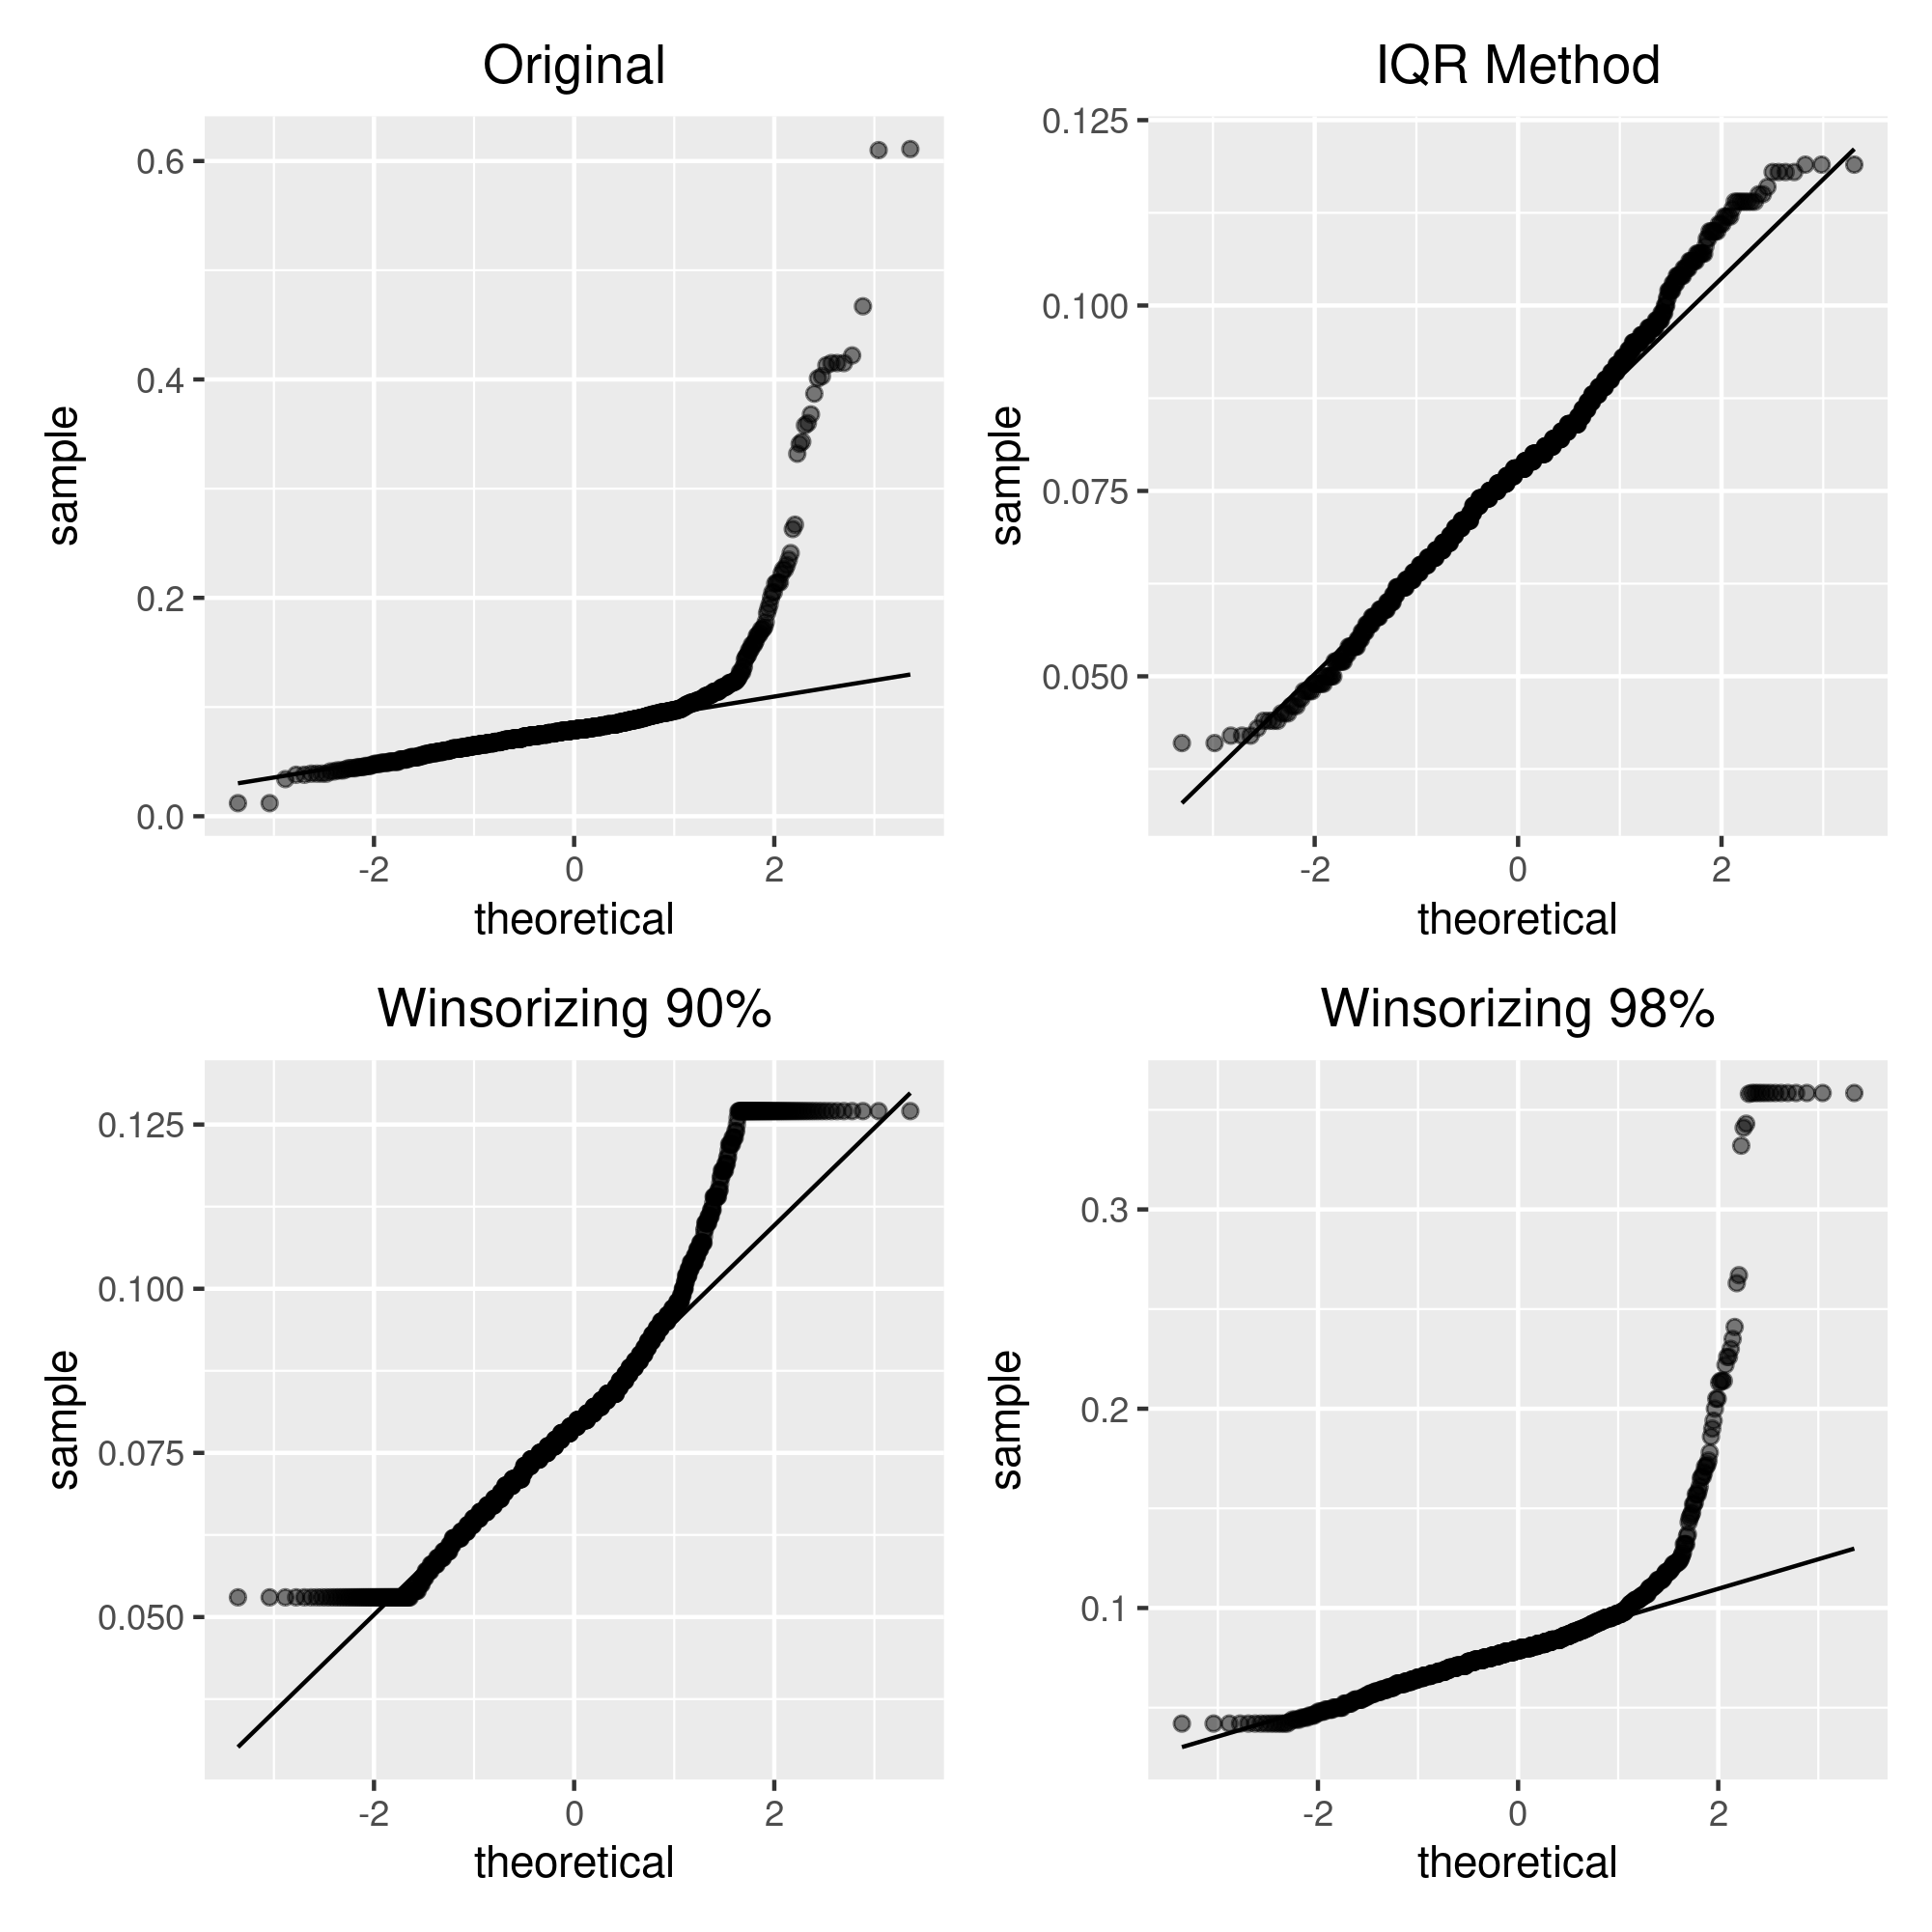
\includegraphics[width=0.45\textwidth]{images/outliers/chlorides_qqplot.png}
    }

    \label{fig:chlorides}
    \caption{Commento}
\end{figure}

\begin{figure}[H]
    \centering

    \subfloat[]{%
        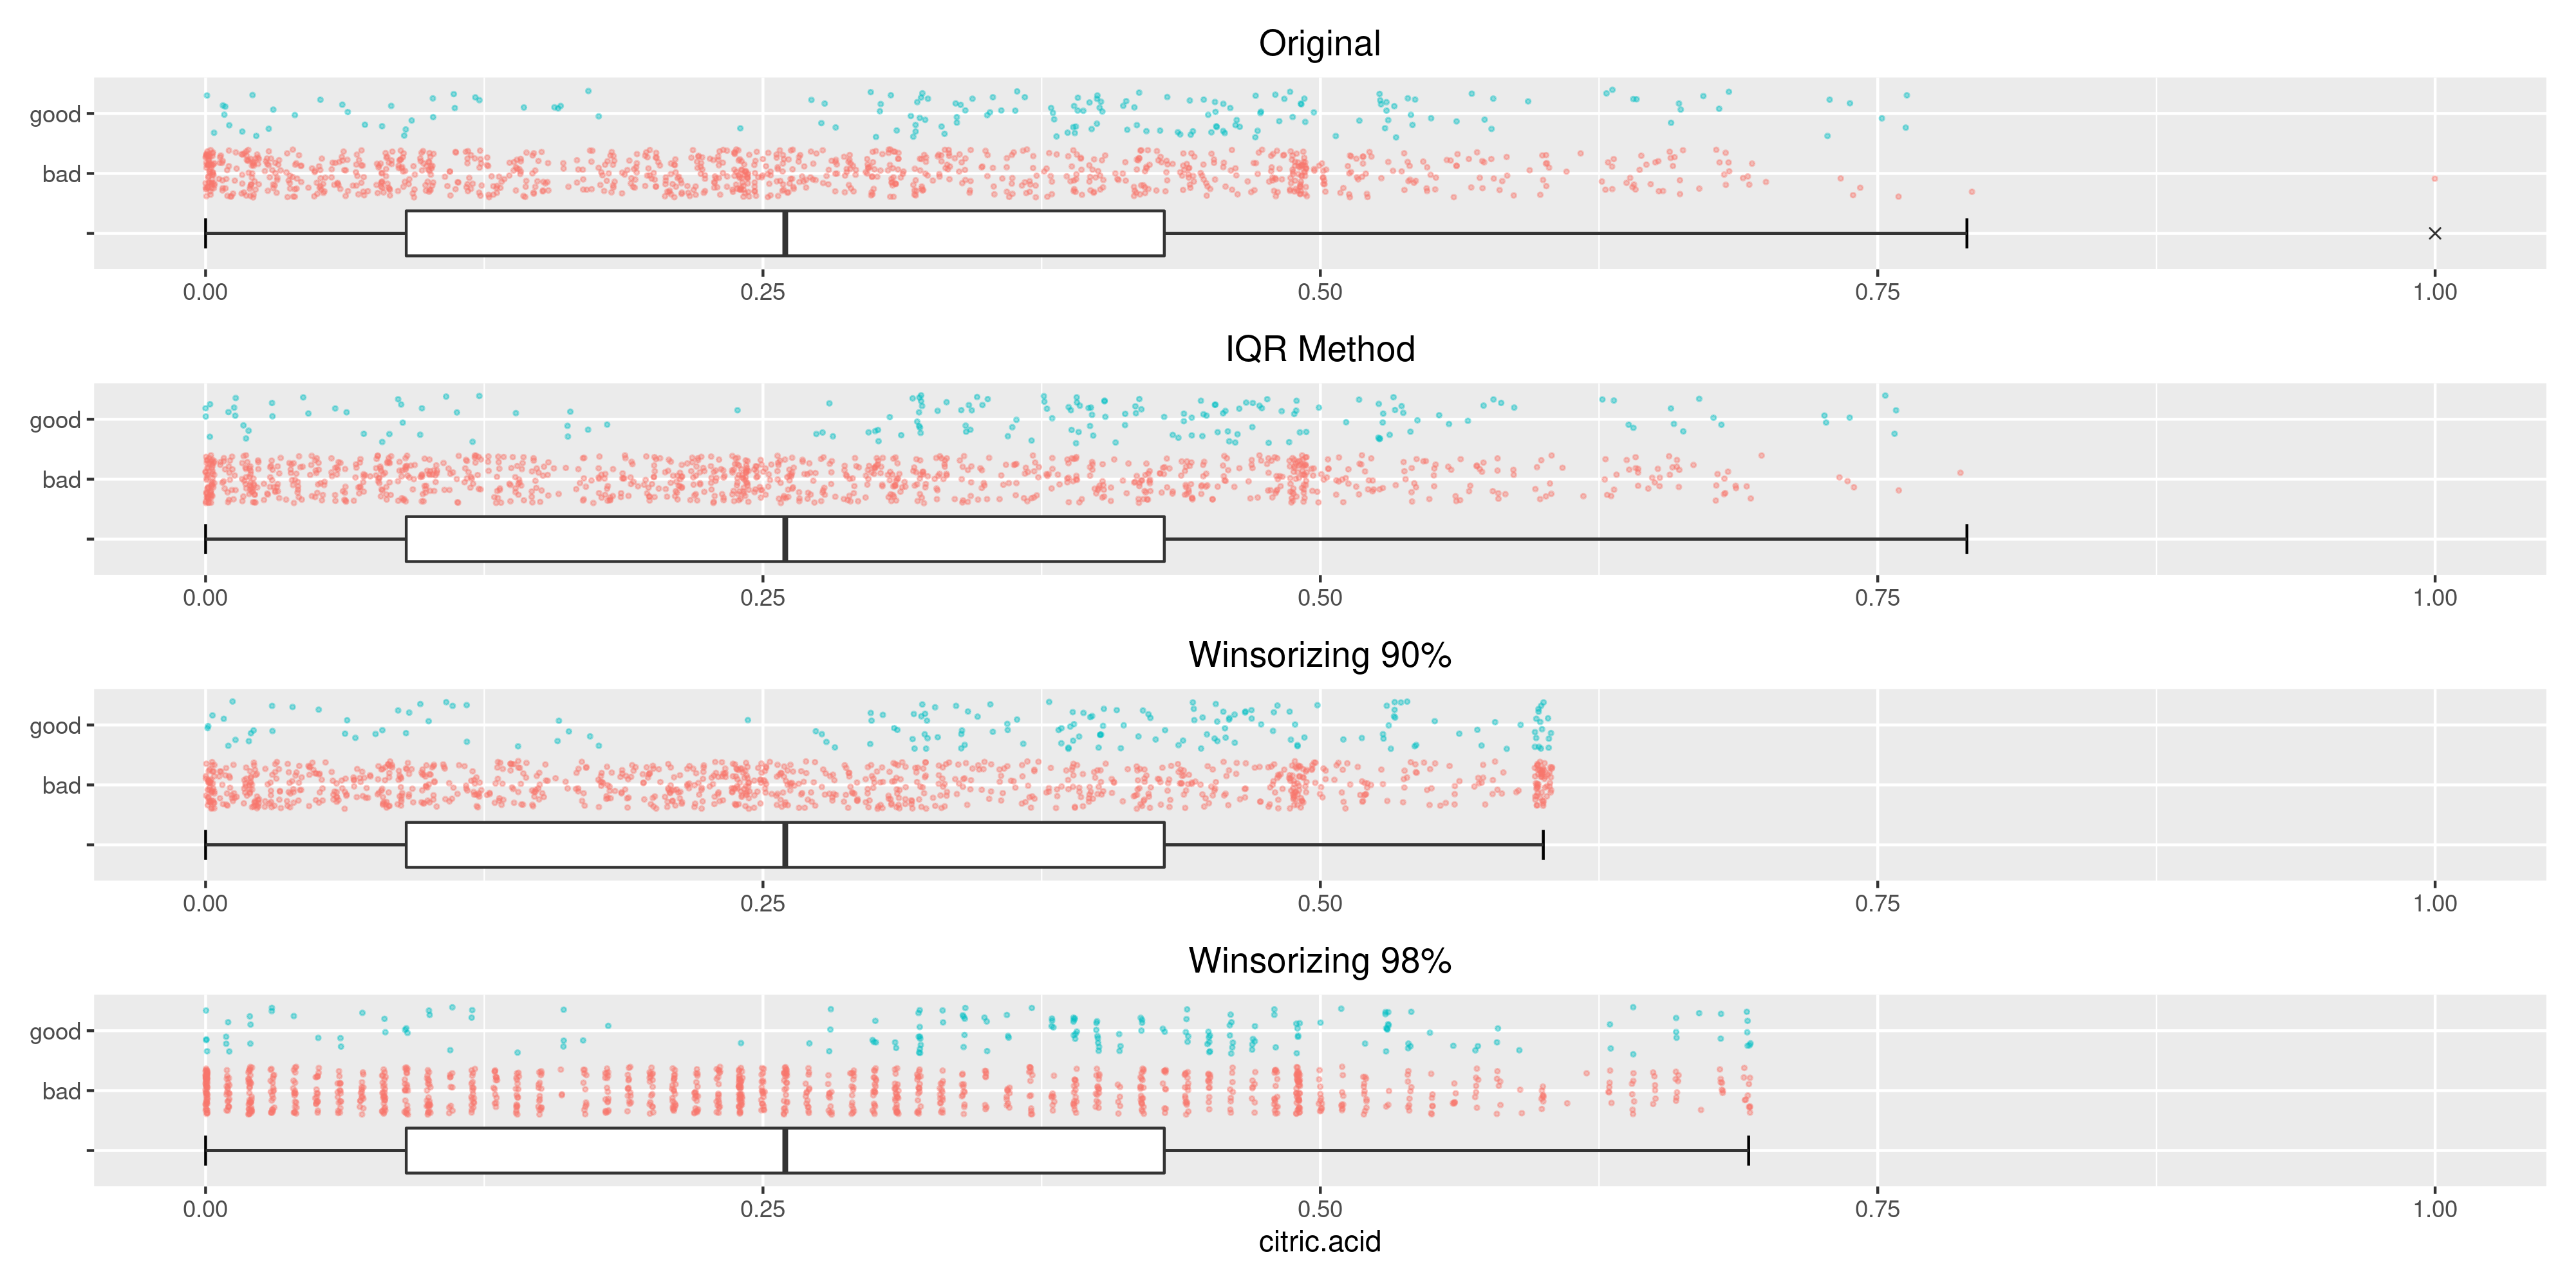
\includegraphics[width=0.99\textwidth]{images/outliers/citric.acid_boxplot.png}
    }

    \subfloat[]{%
        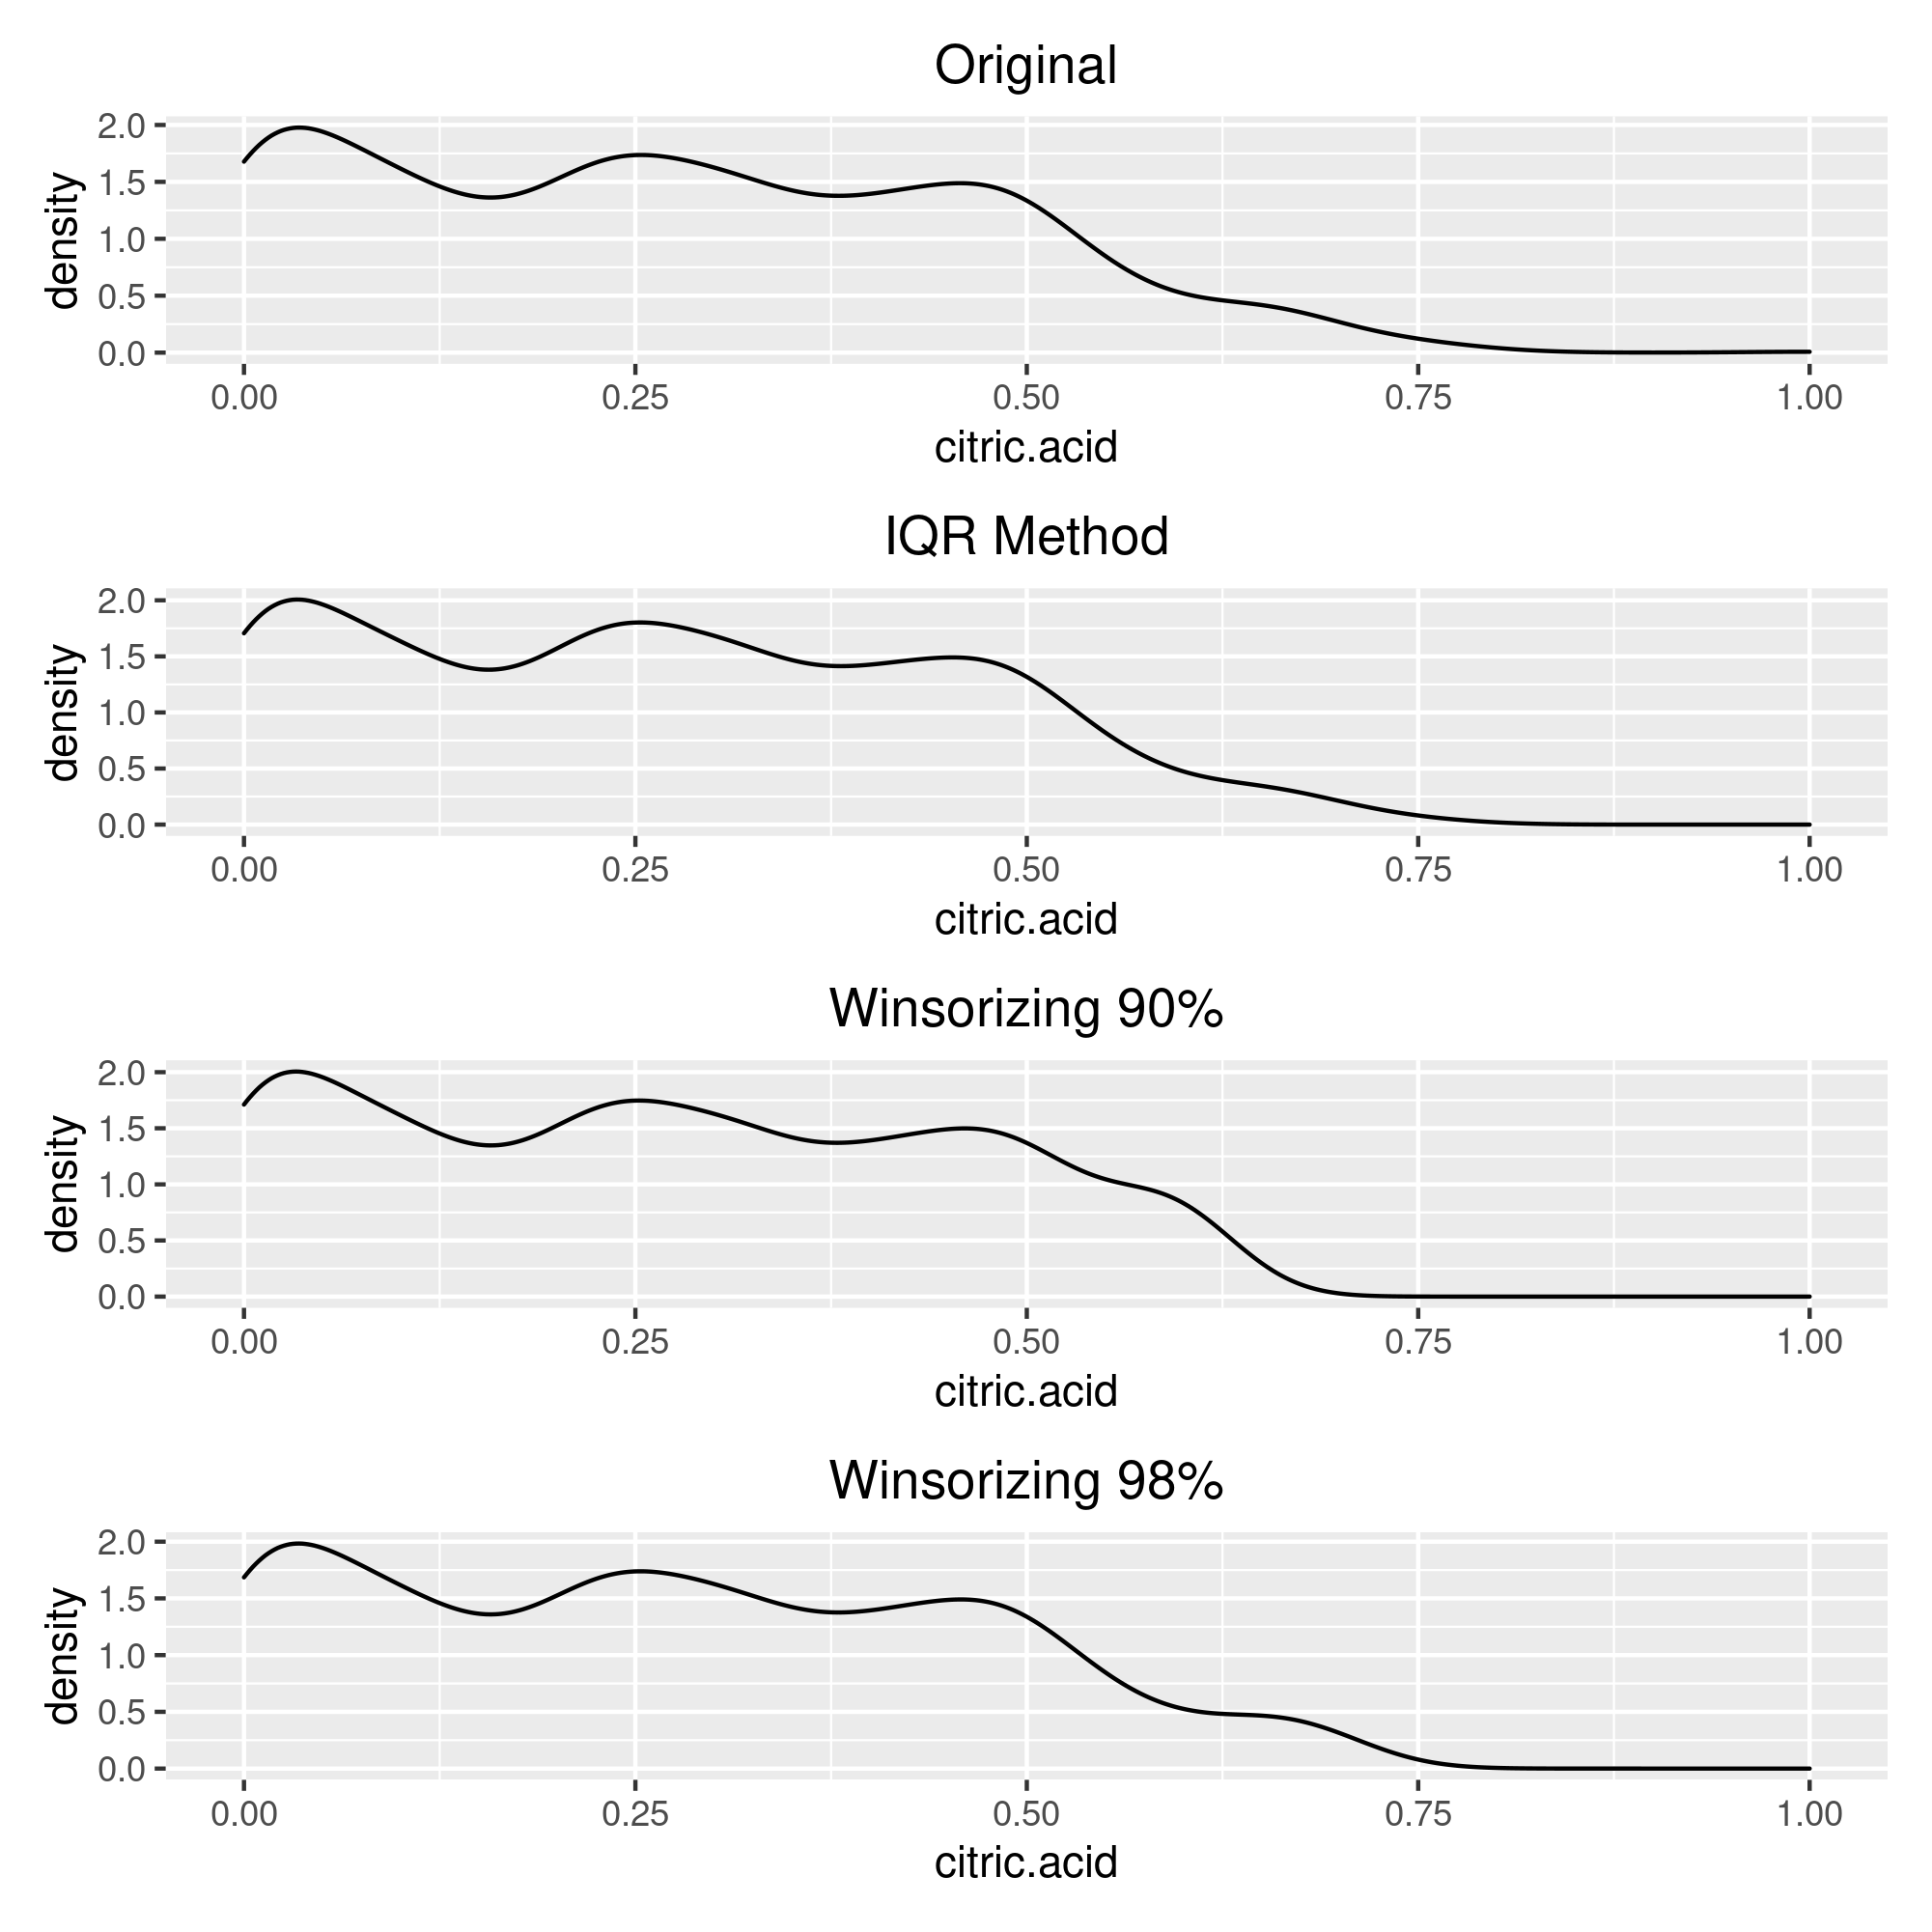
\includegraphics[width=0.45\textwidth]{images/outliers/citric.acid_distribution.png}
    }\qquad
    \subfloat[]{%
        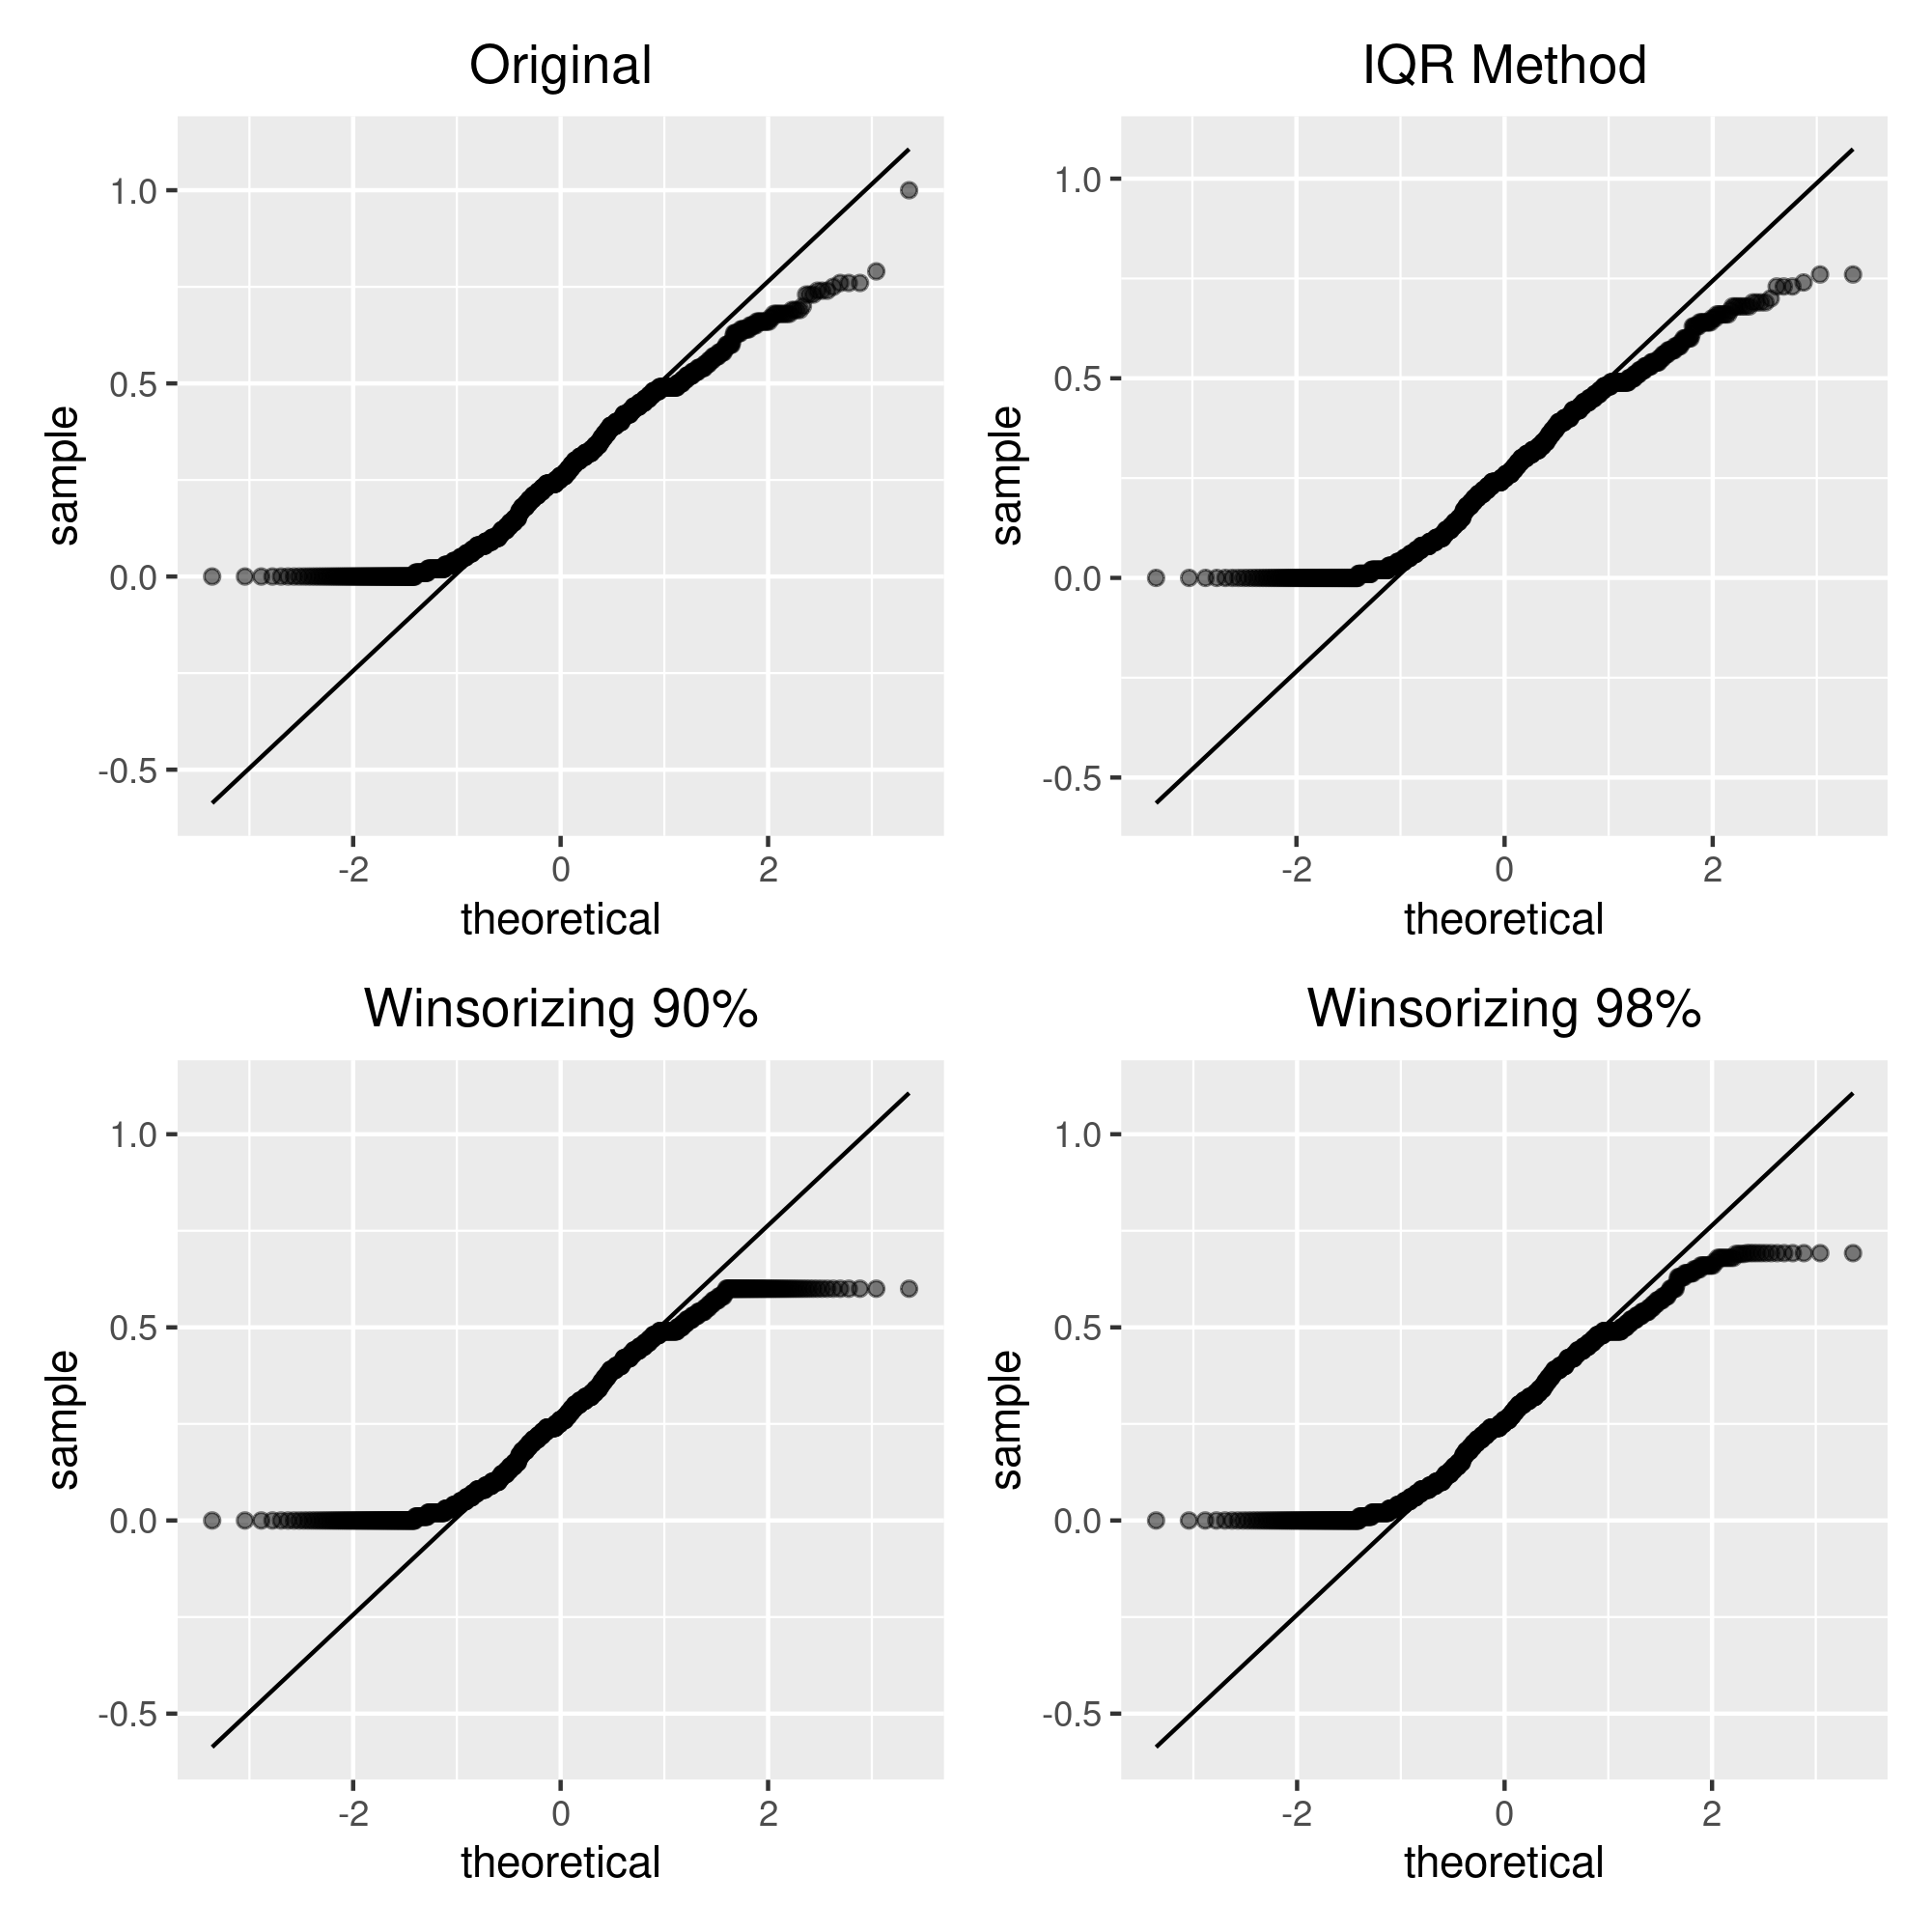
\includegraphics[width=0.45\textwidth]{images/outliers/citric.acid_qqplot.png}
    }

    \label{fig:citric.acid}
    \caption{Commento}
\end{figure}

\begin{figure}[H]
    \centering

    \subfloat[]{%
        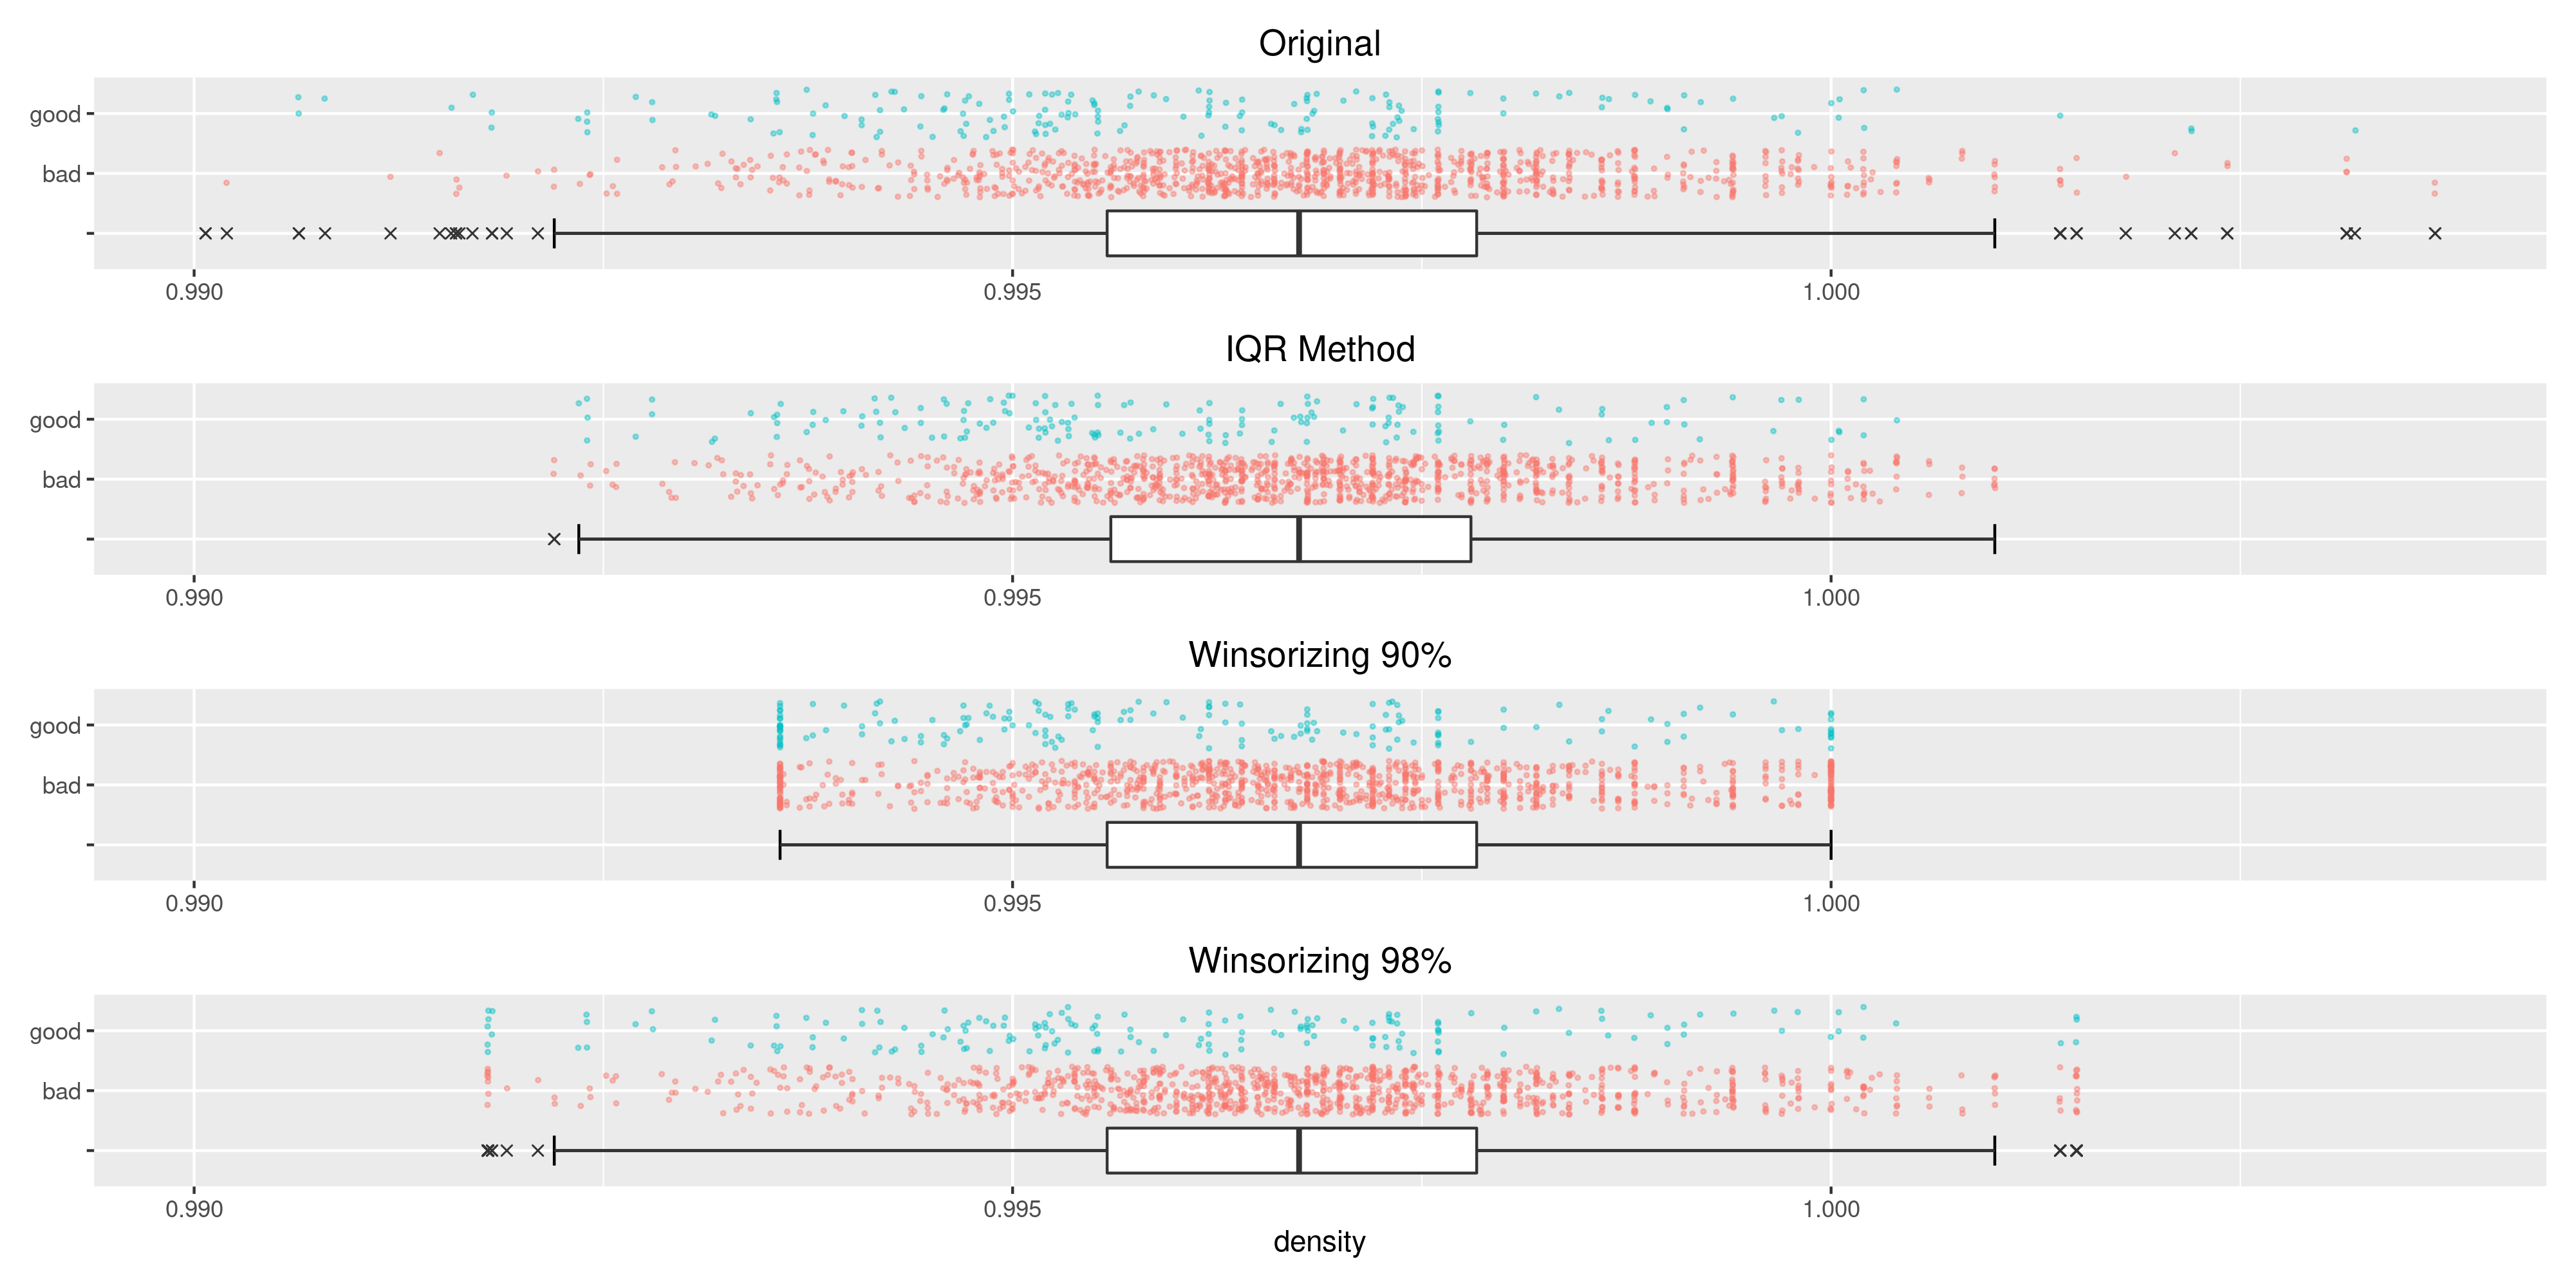
\includegraphics[width=0.99\textwidth]{images/outliers/density_boxplot.png}
    }

    \subfloat[]{%
        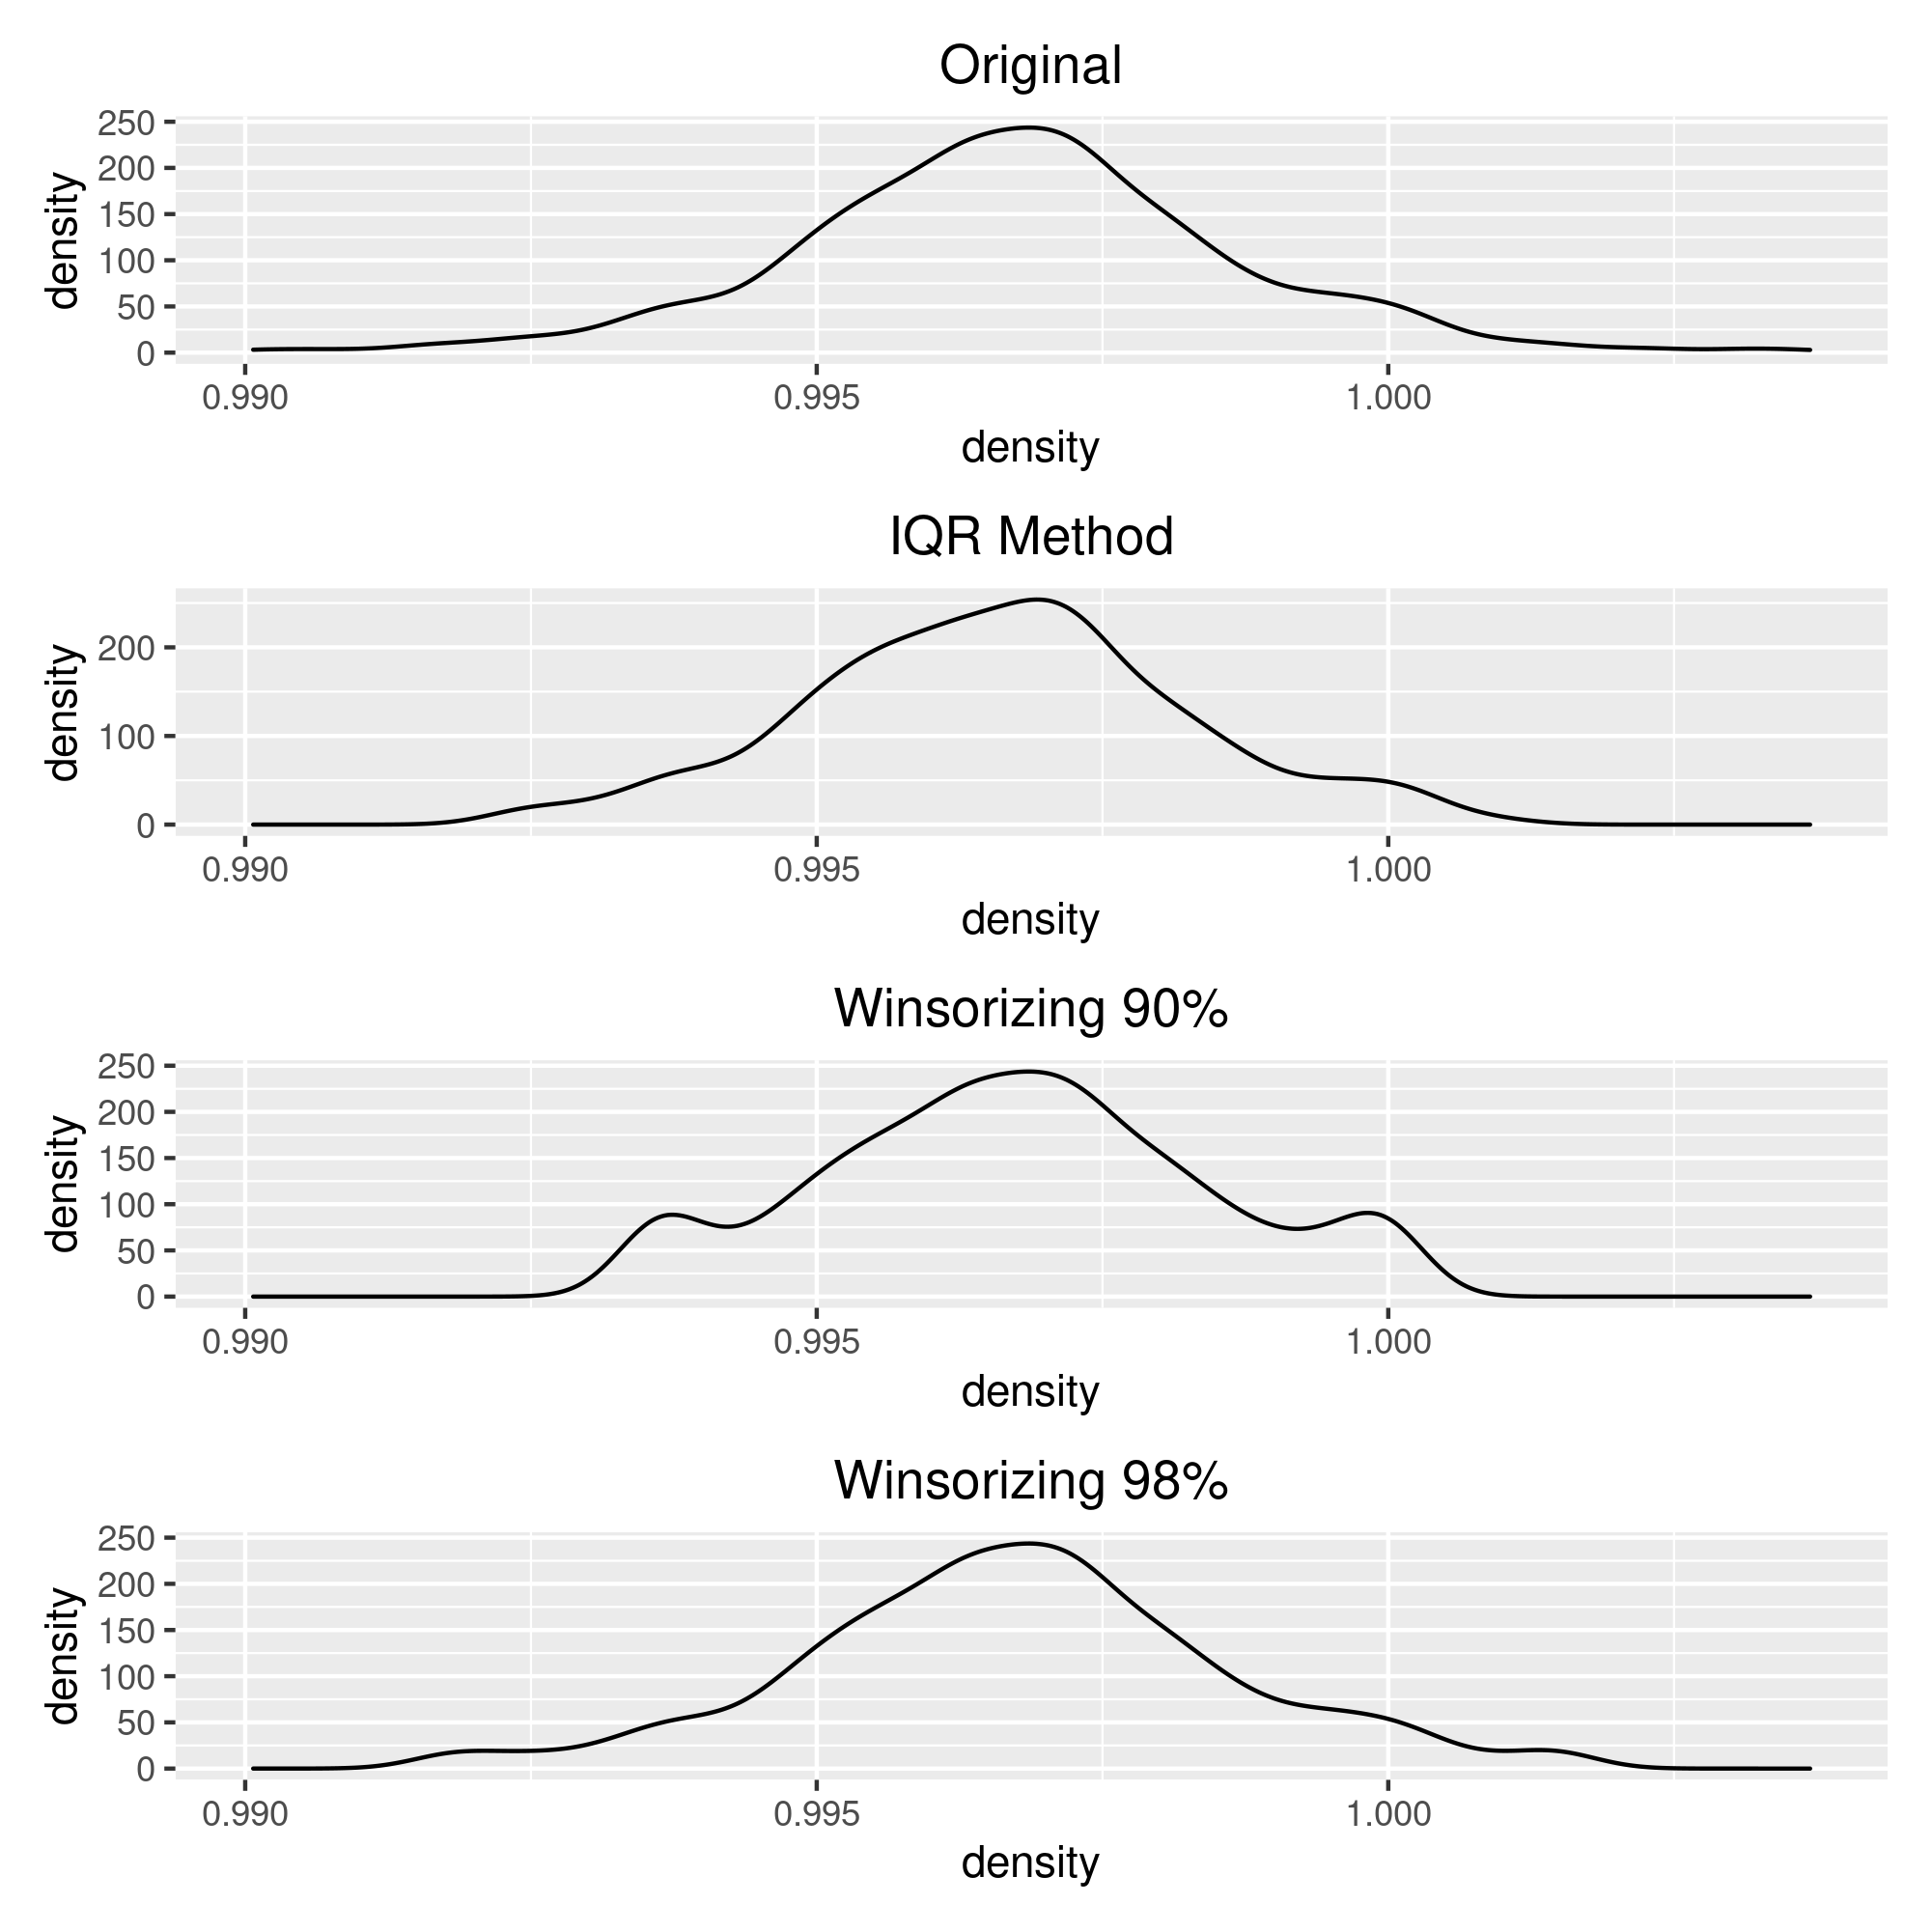
\includegraphics[width=0.45\textwidth]{images/outliers/density_distribution.png}
    }\qquad
    \subfloat[]{%
        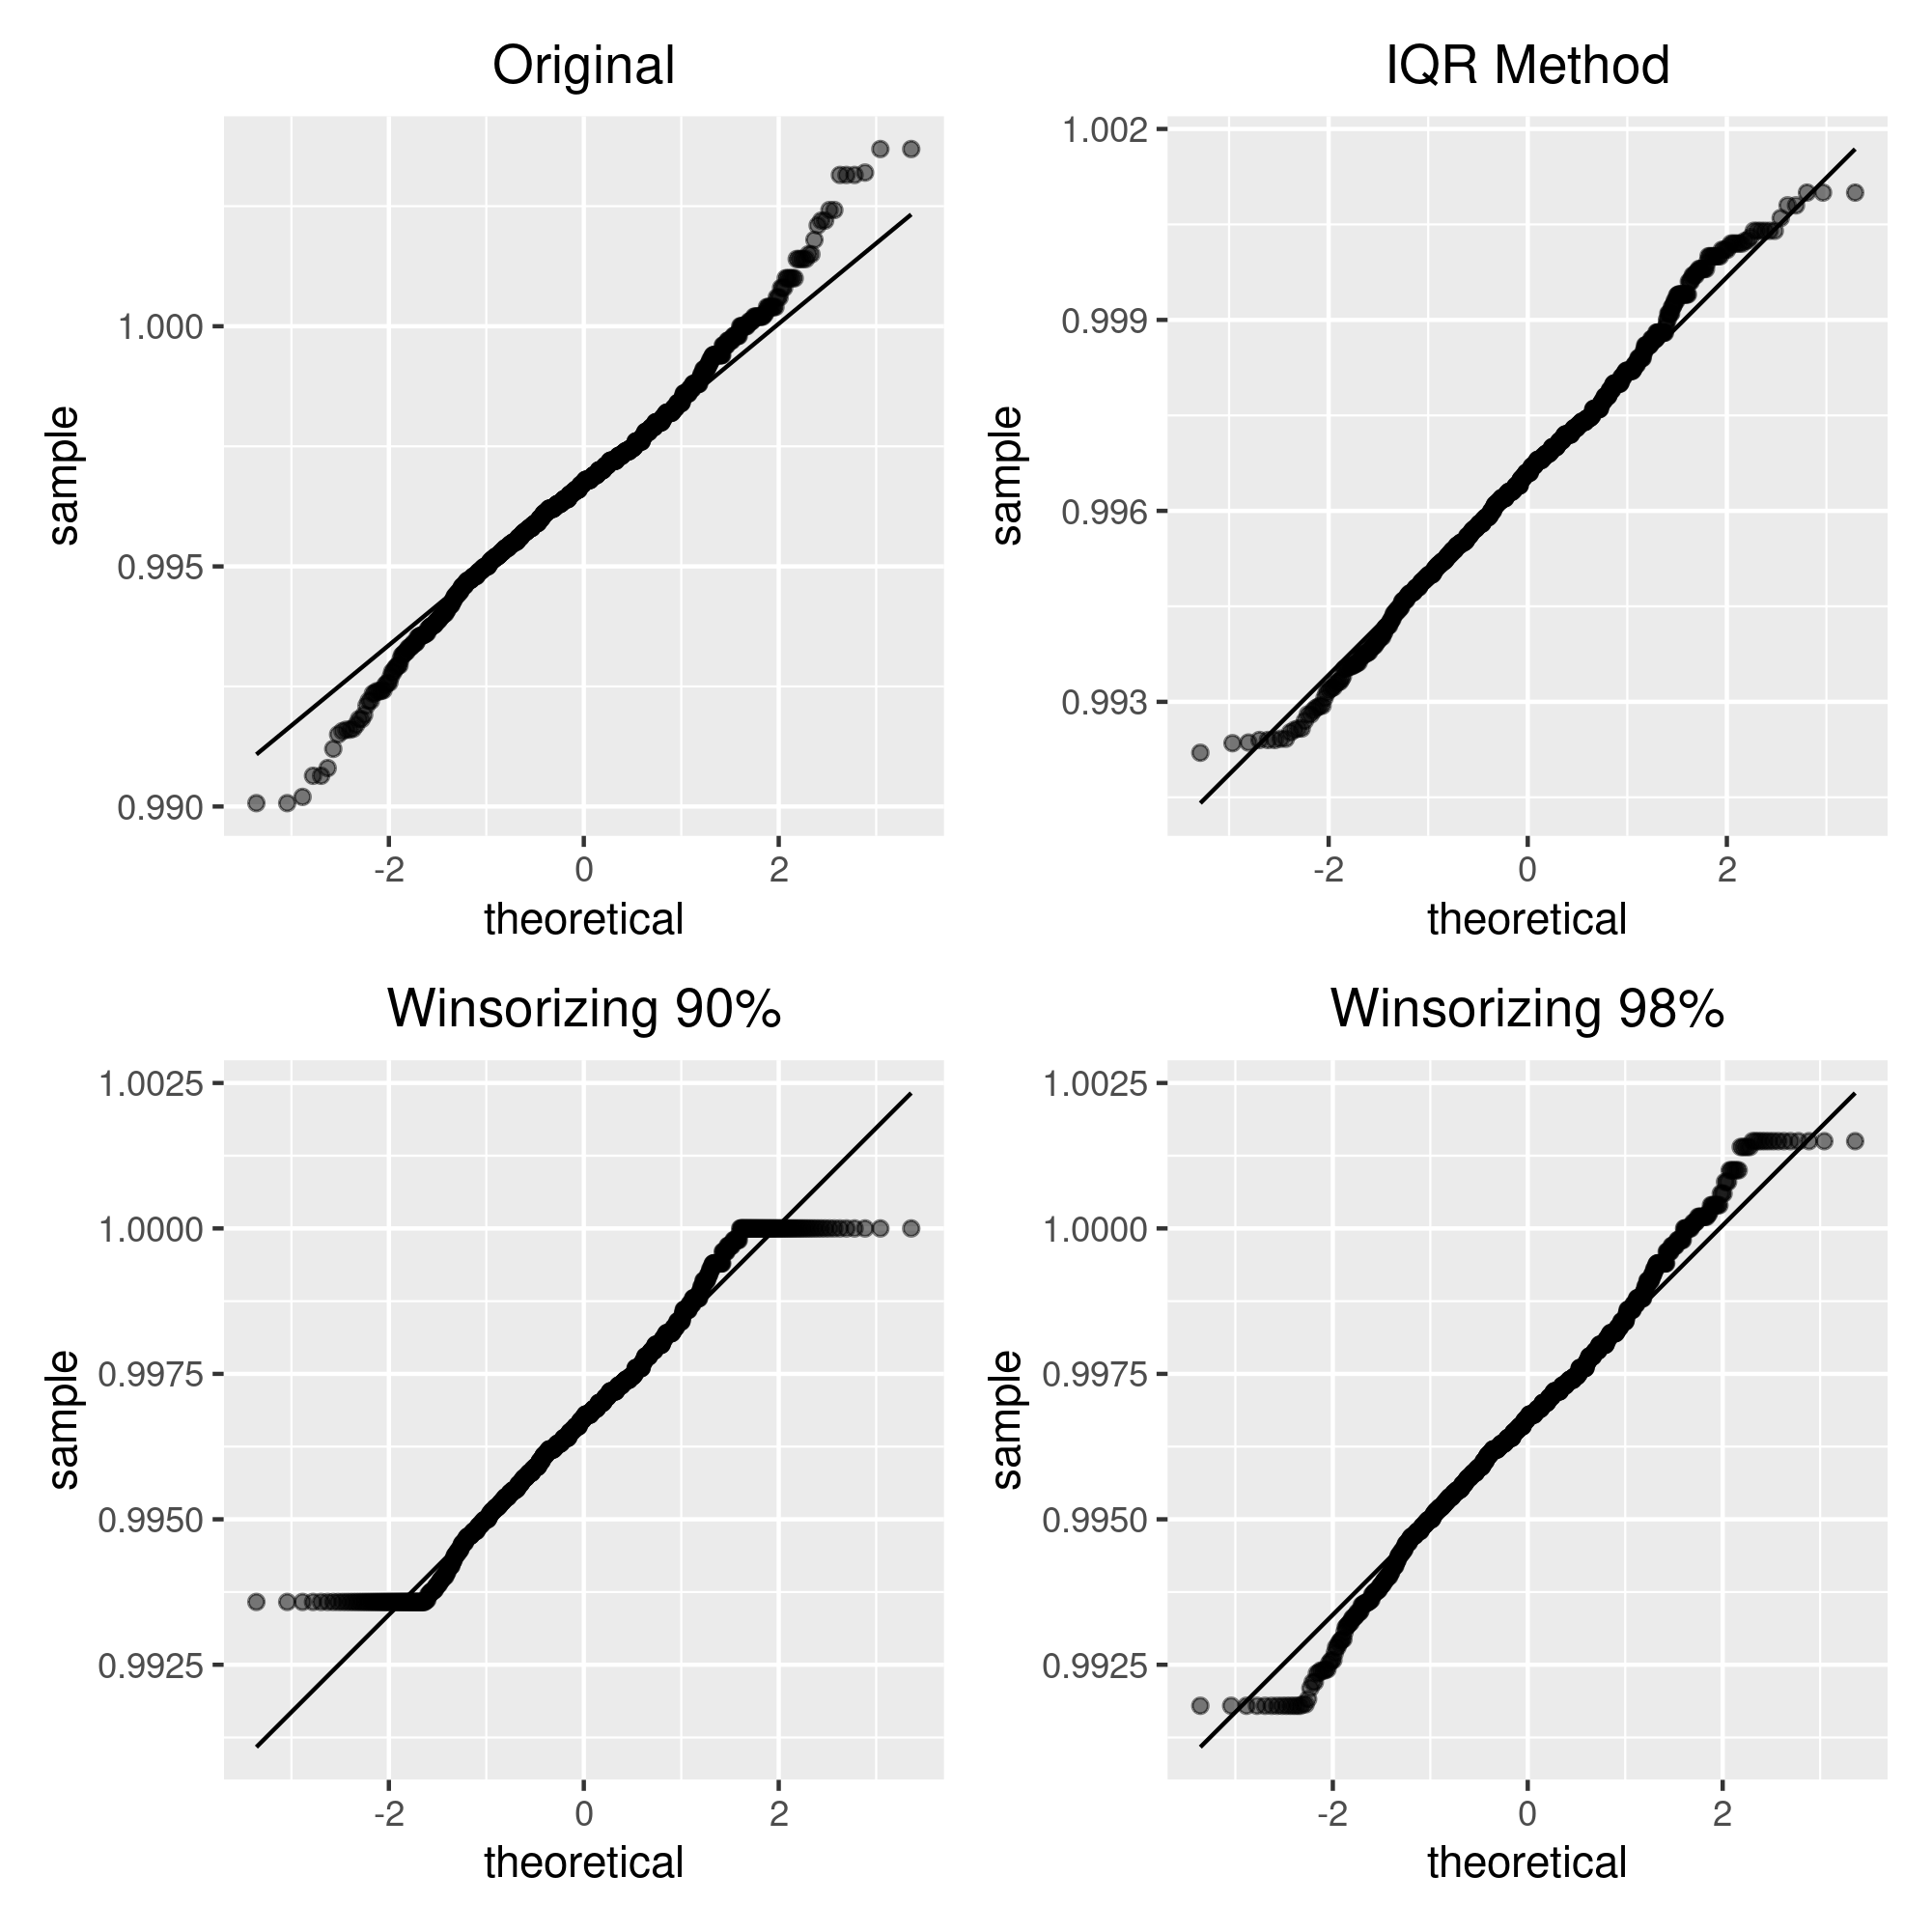
\includegraphics[width=0.45\textwidth]{images/outliers/density_qqplot.png}
    }

    \label{fig:density}
    \caption{Commento}
\end{figure}

\begin{figure}[H]
    \centering

    \subfloat[]{%
        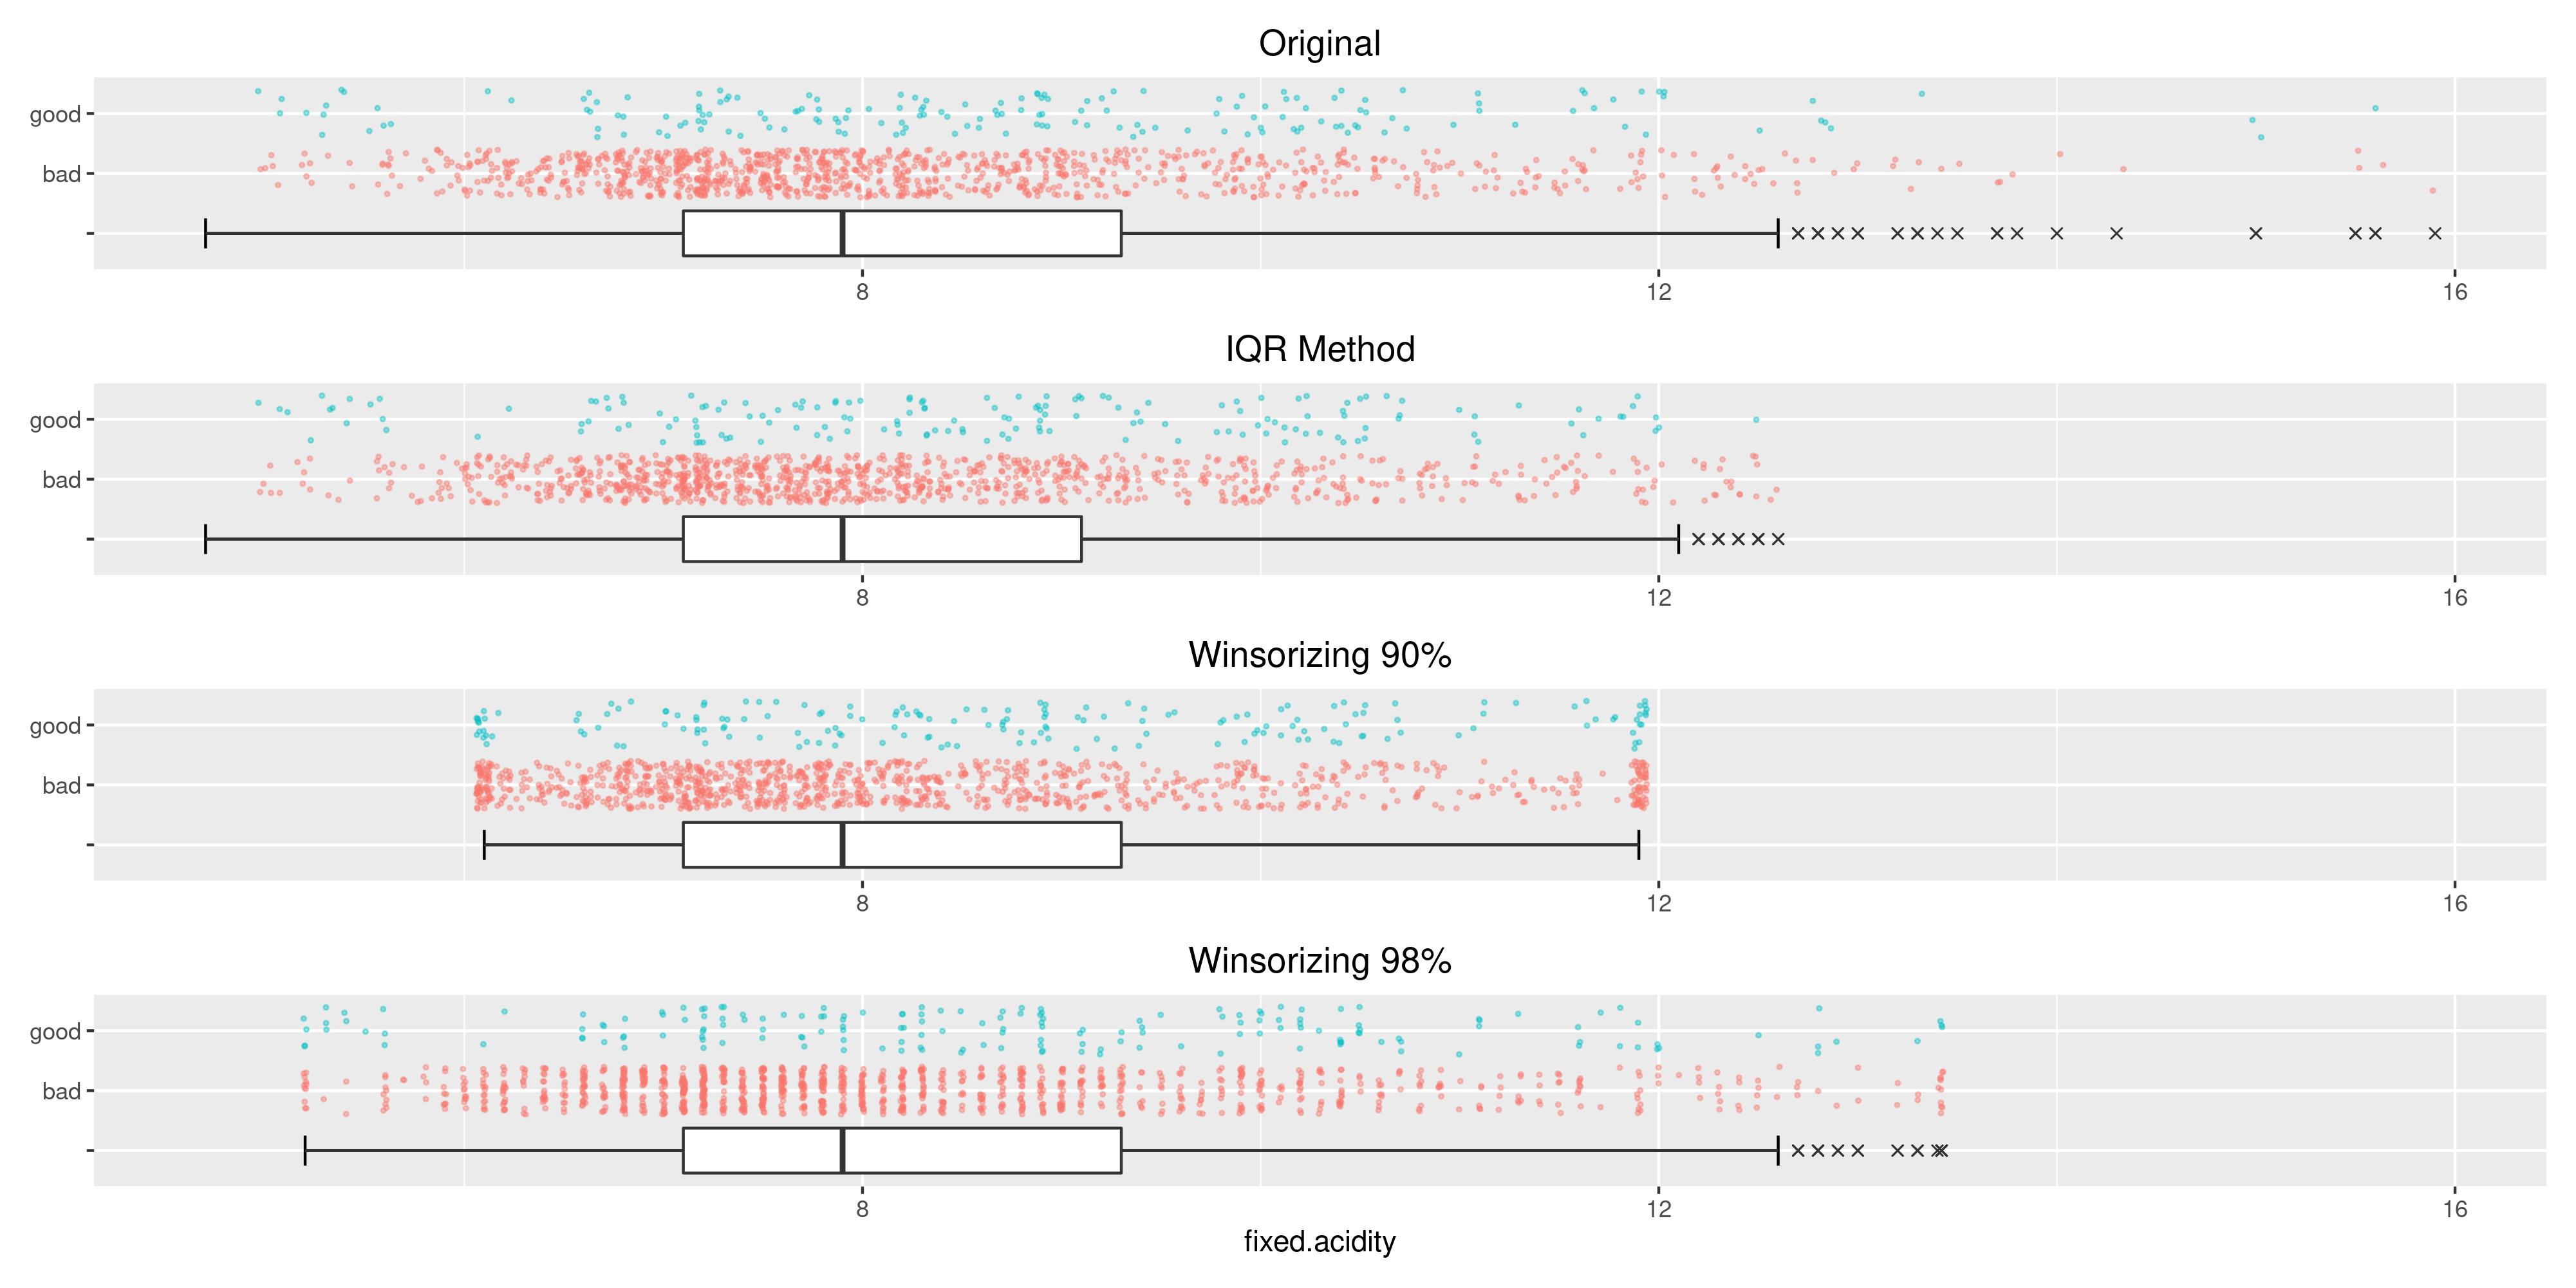
\includegraphics[width=0.99\textwidth]{images/outliers/fixed.acidity_boxplot.png}
    }

    \subfloat[]{%
        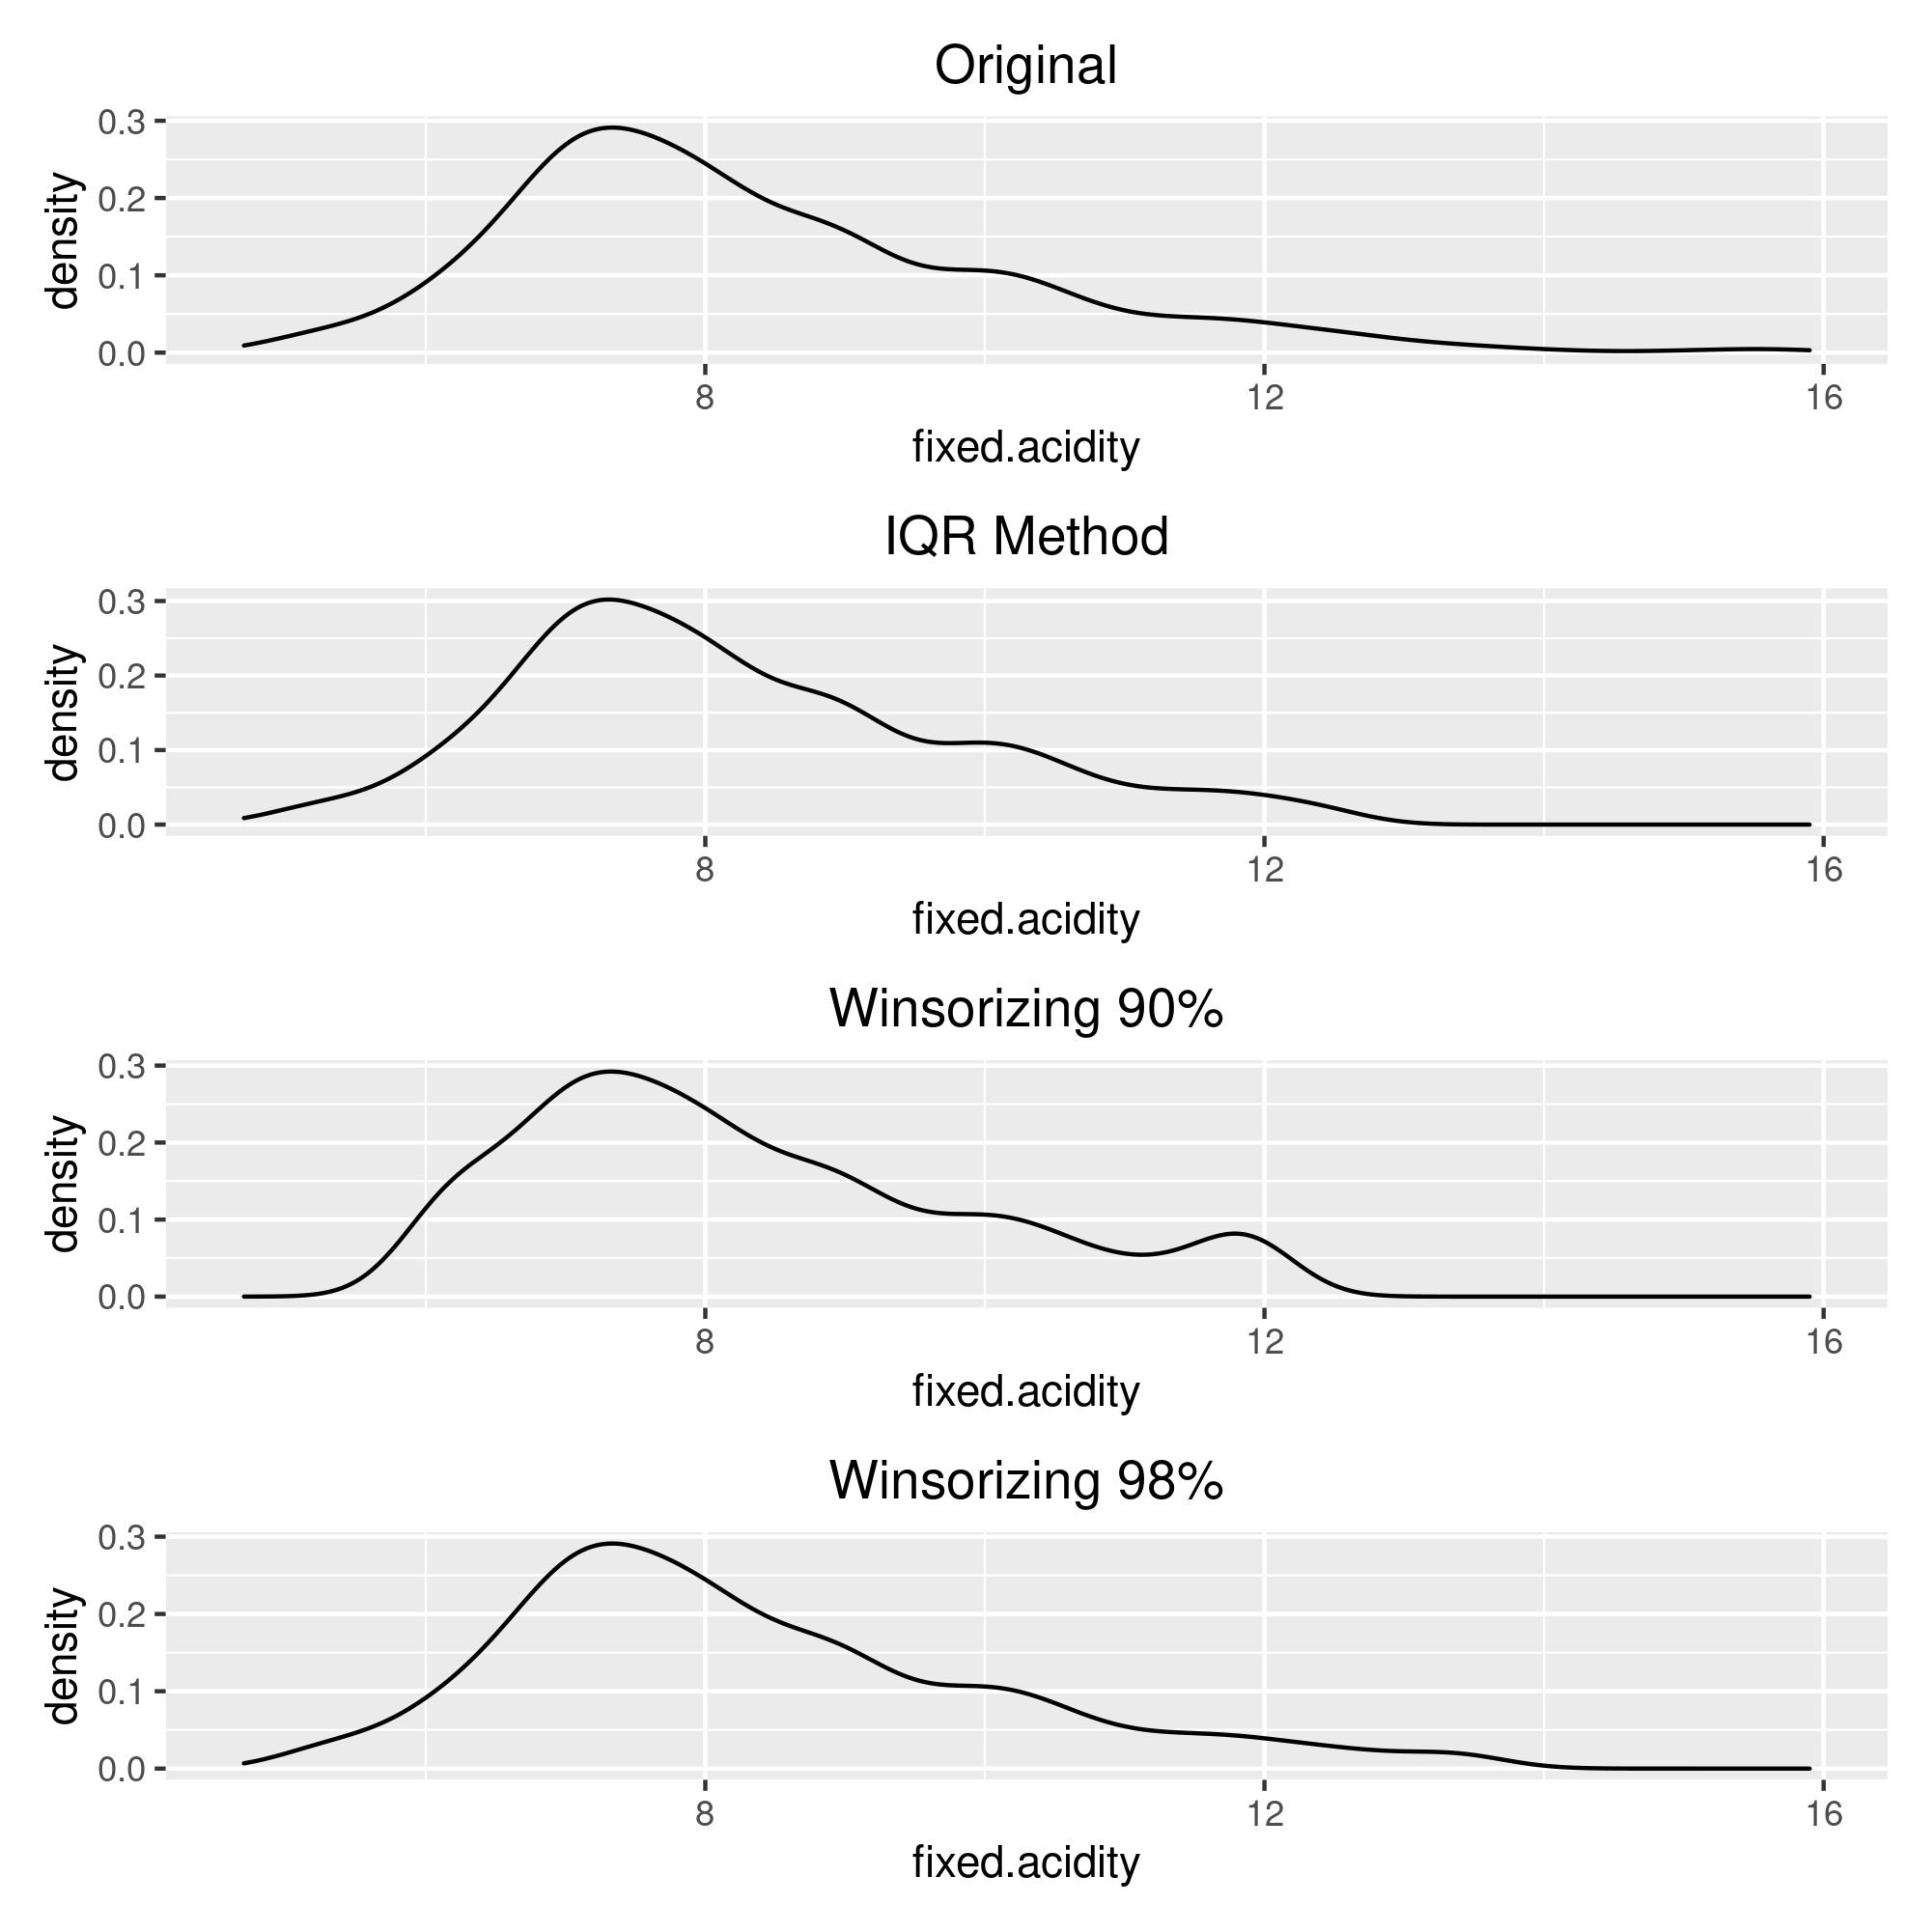
\includegraphics[width=0.45\textwidth]{images/outliers/fixed.acidity_distribution.png}
    }\qquad
    \subfloat[]{%
        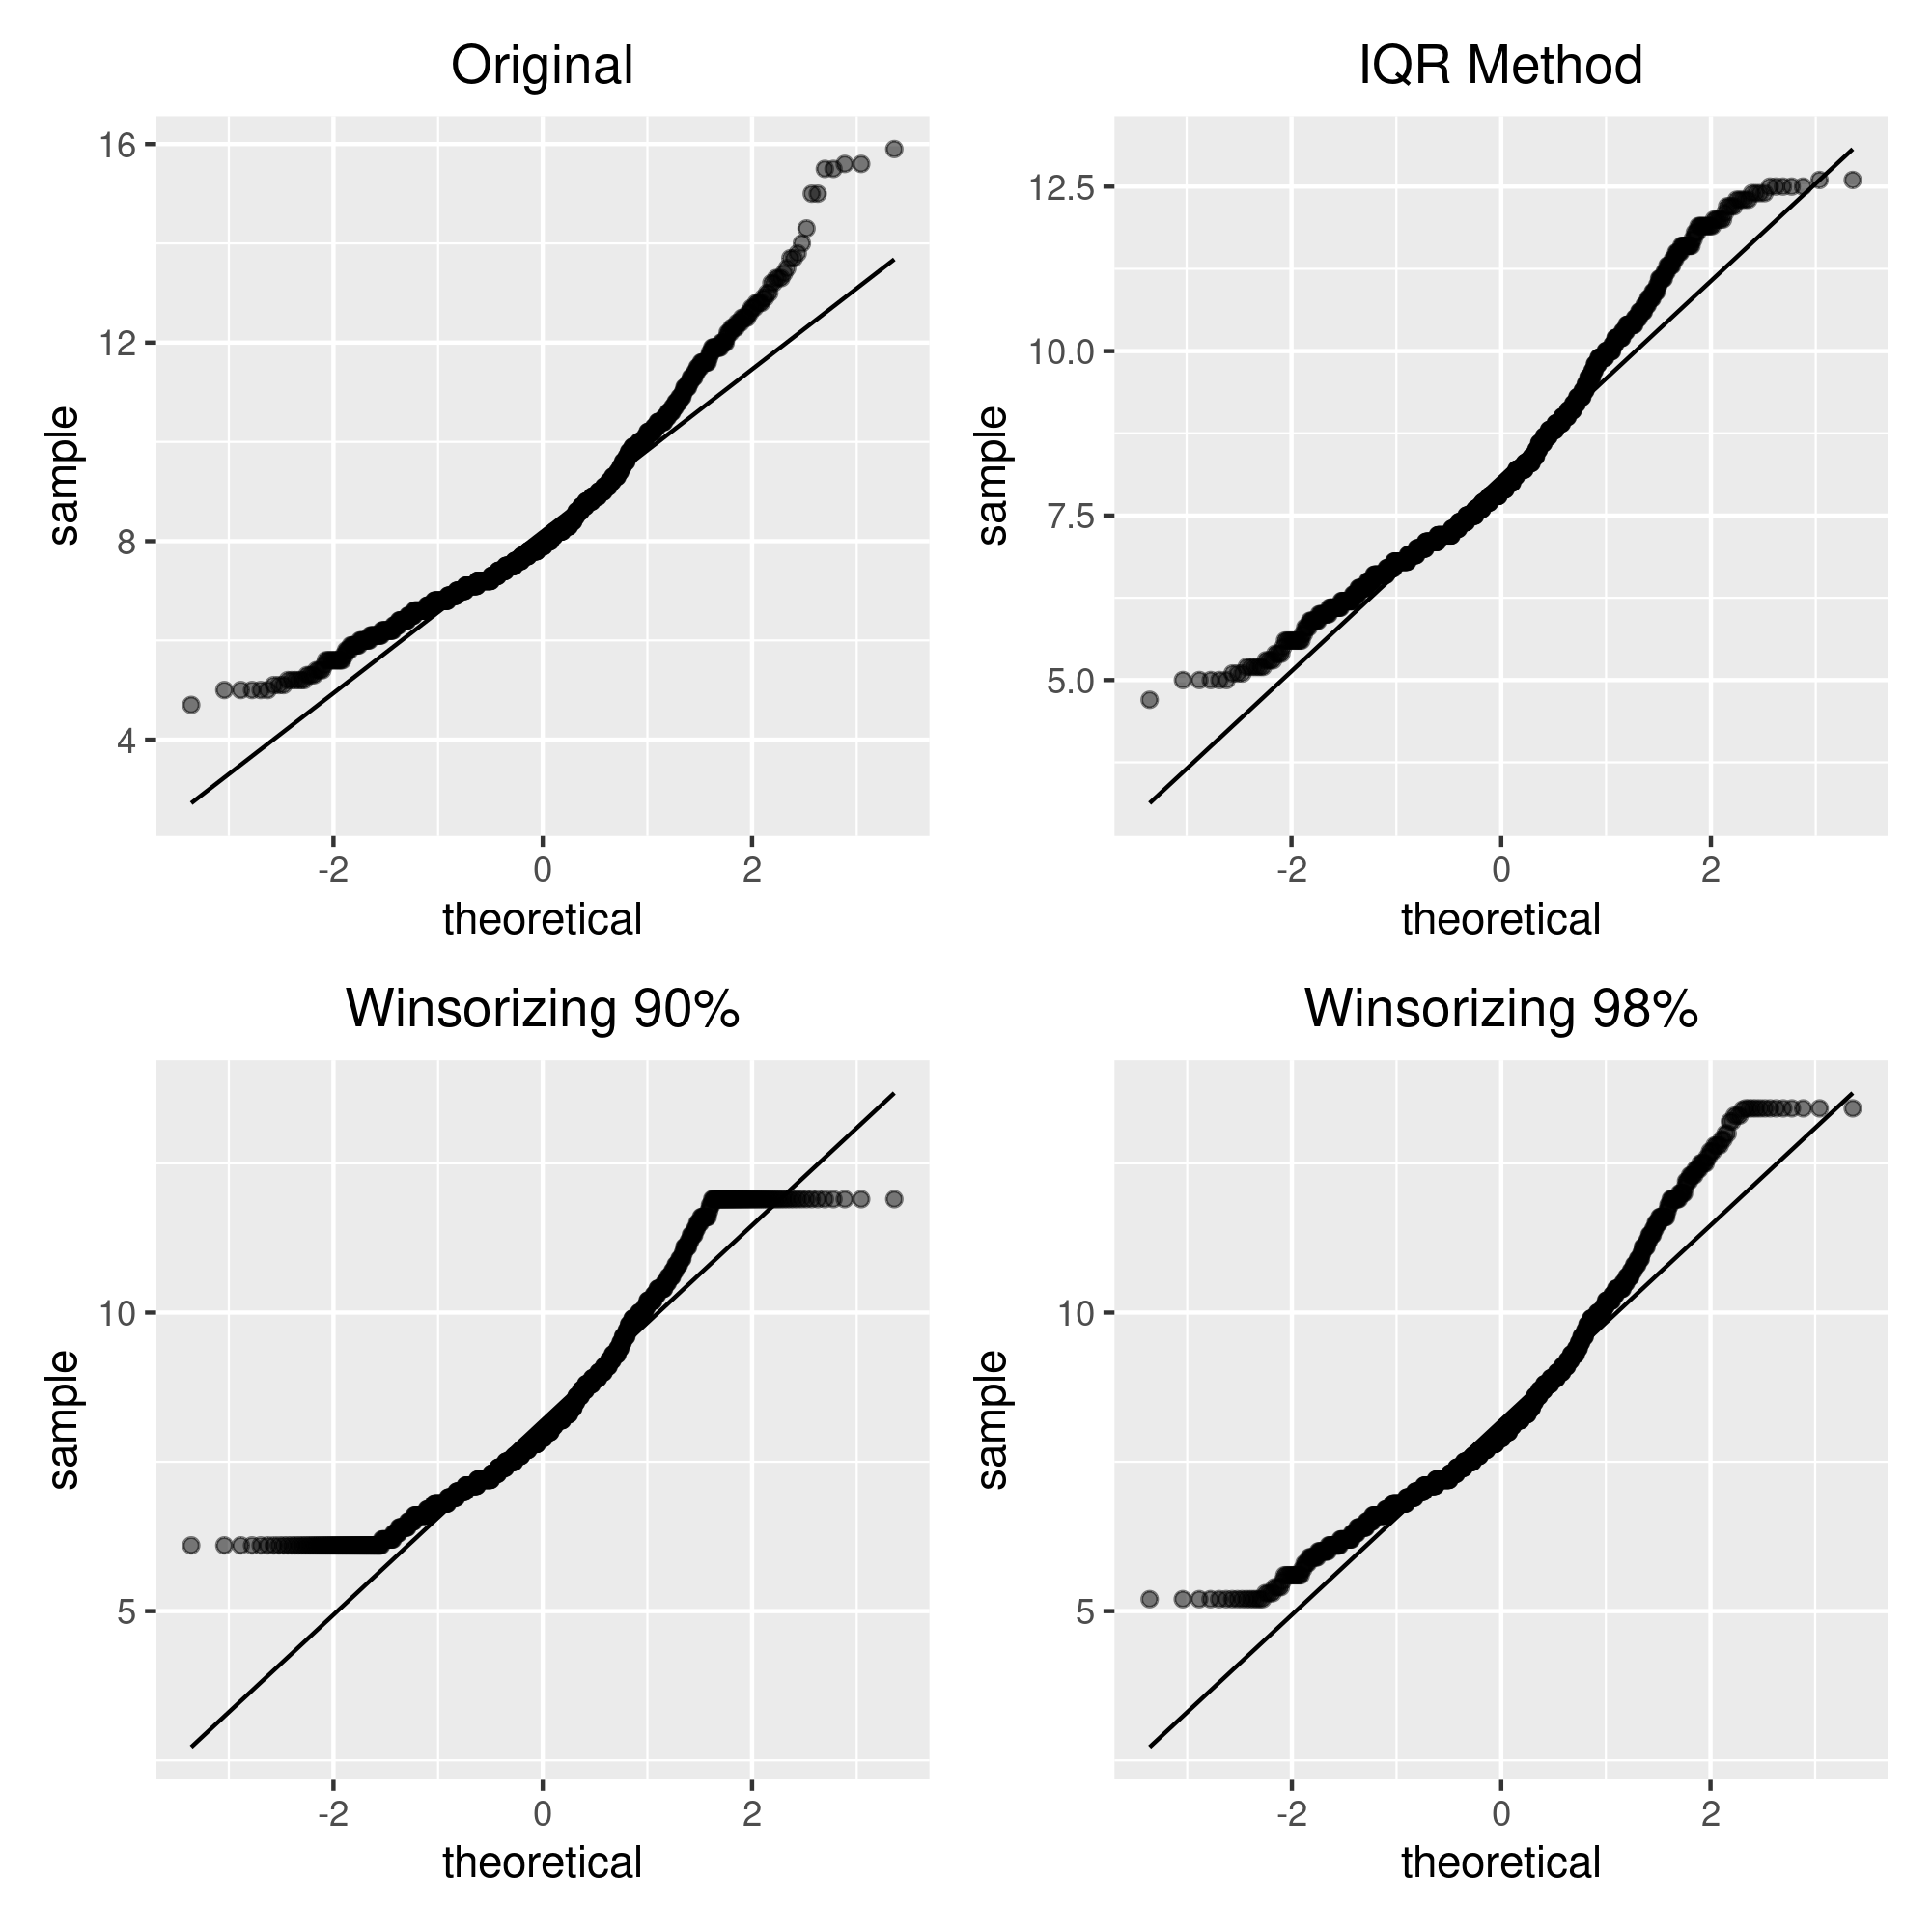
\includegraphics[width=0.45\textwidth]{images/outliers/fixed.acidity_qqplot.png}
    }

    \label{fig:fixed.acidity}
    \caption{Commento}
\end{figure}

\begin{figure}[H]
    \centering

    \subfloat[]{%
        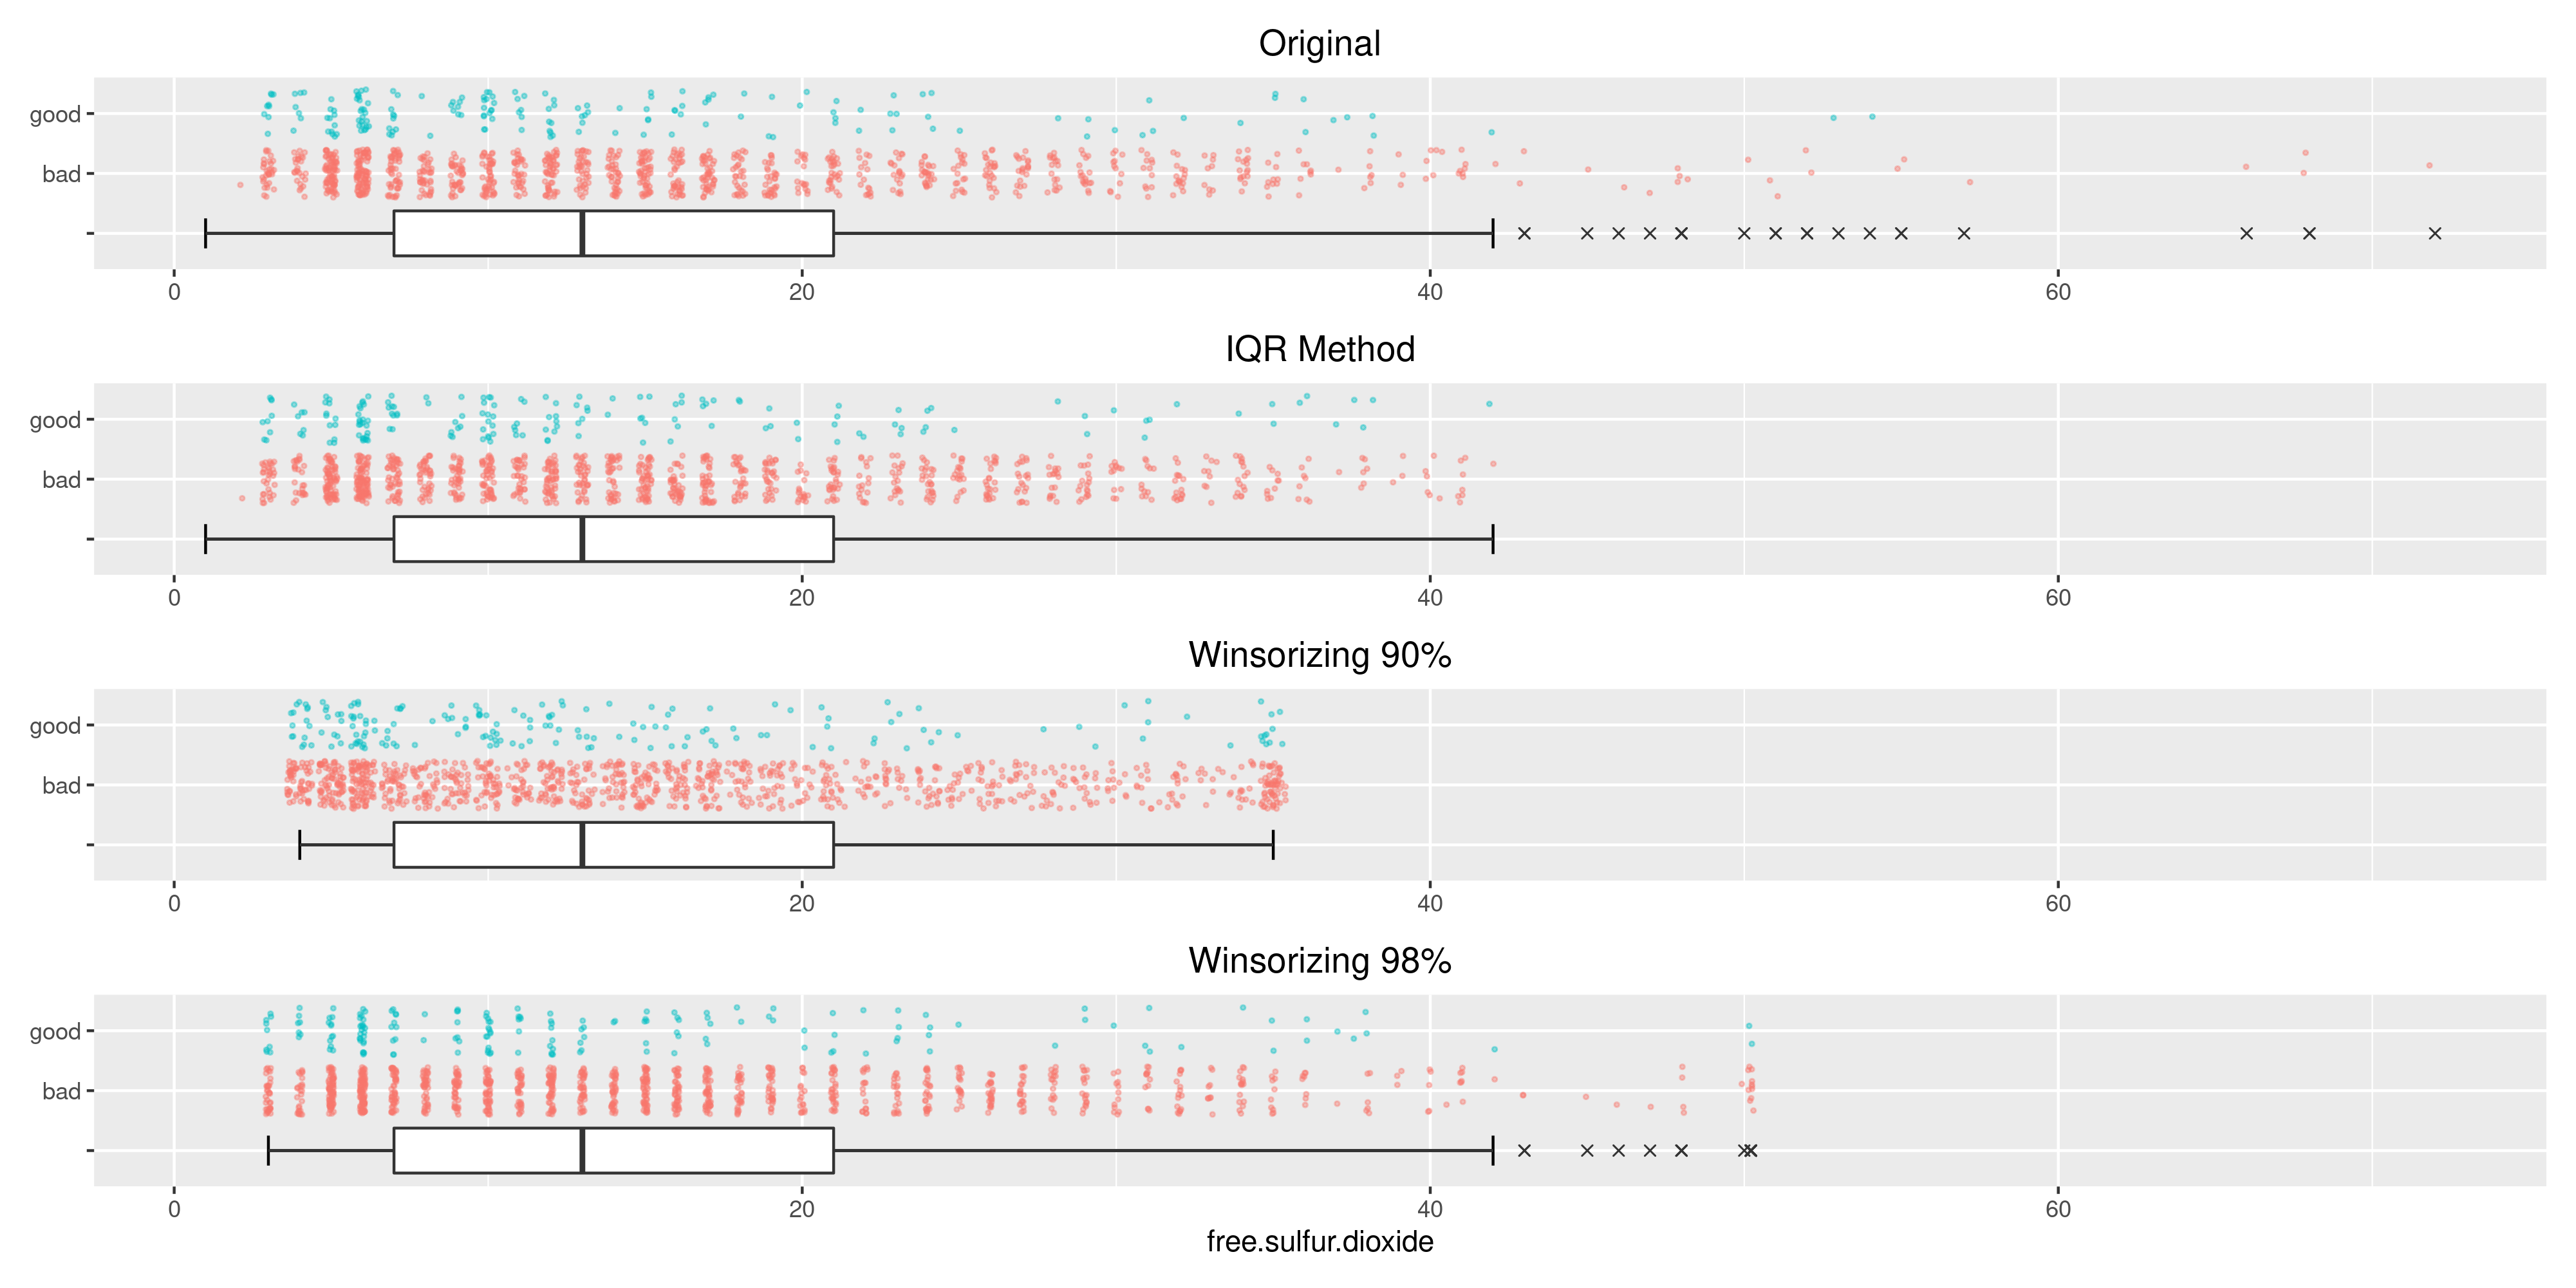
\includegraphics[width=0.99\textwidth]{images/outliers/free.sulfur.dioxide_boxplot.png}
    }

    \subfloat[]{%
        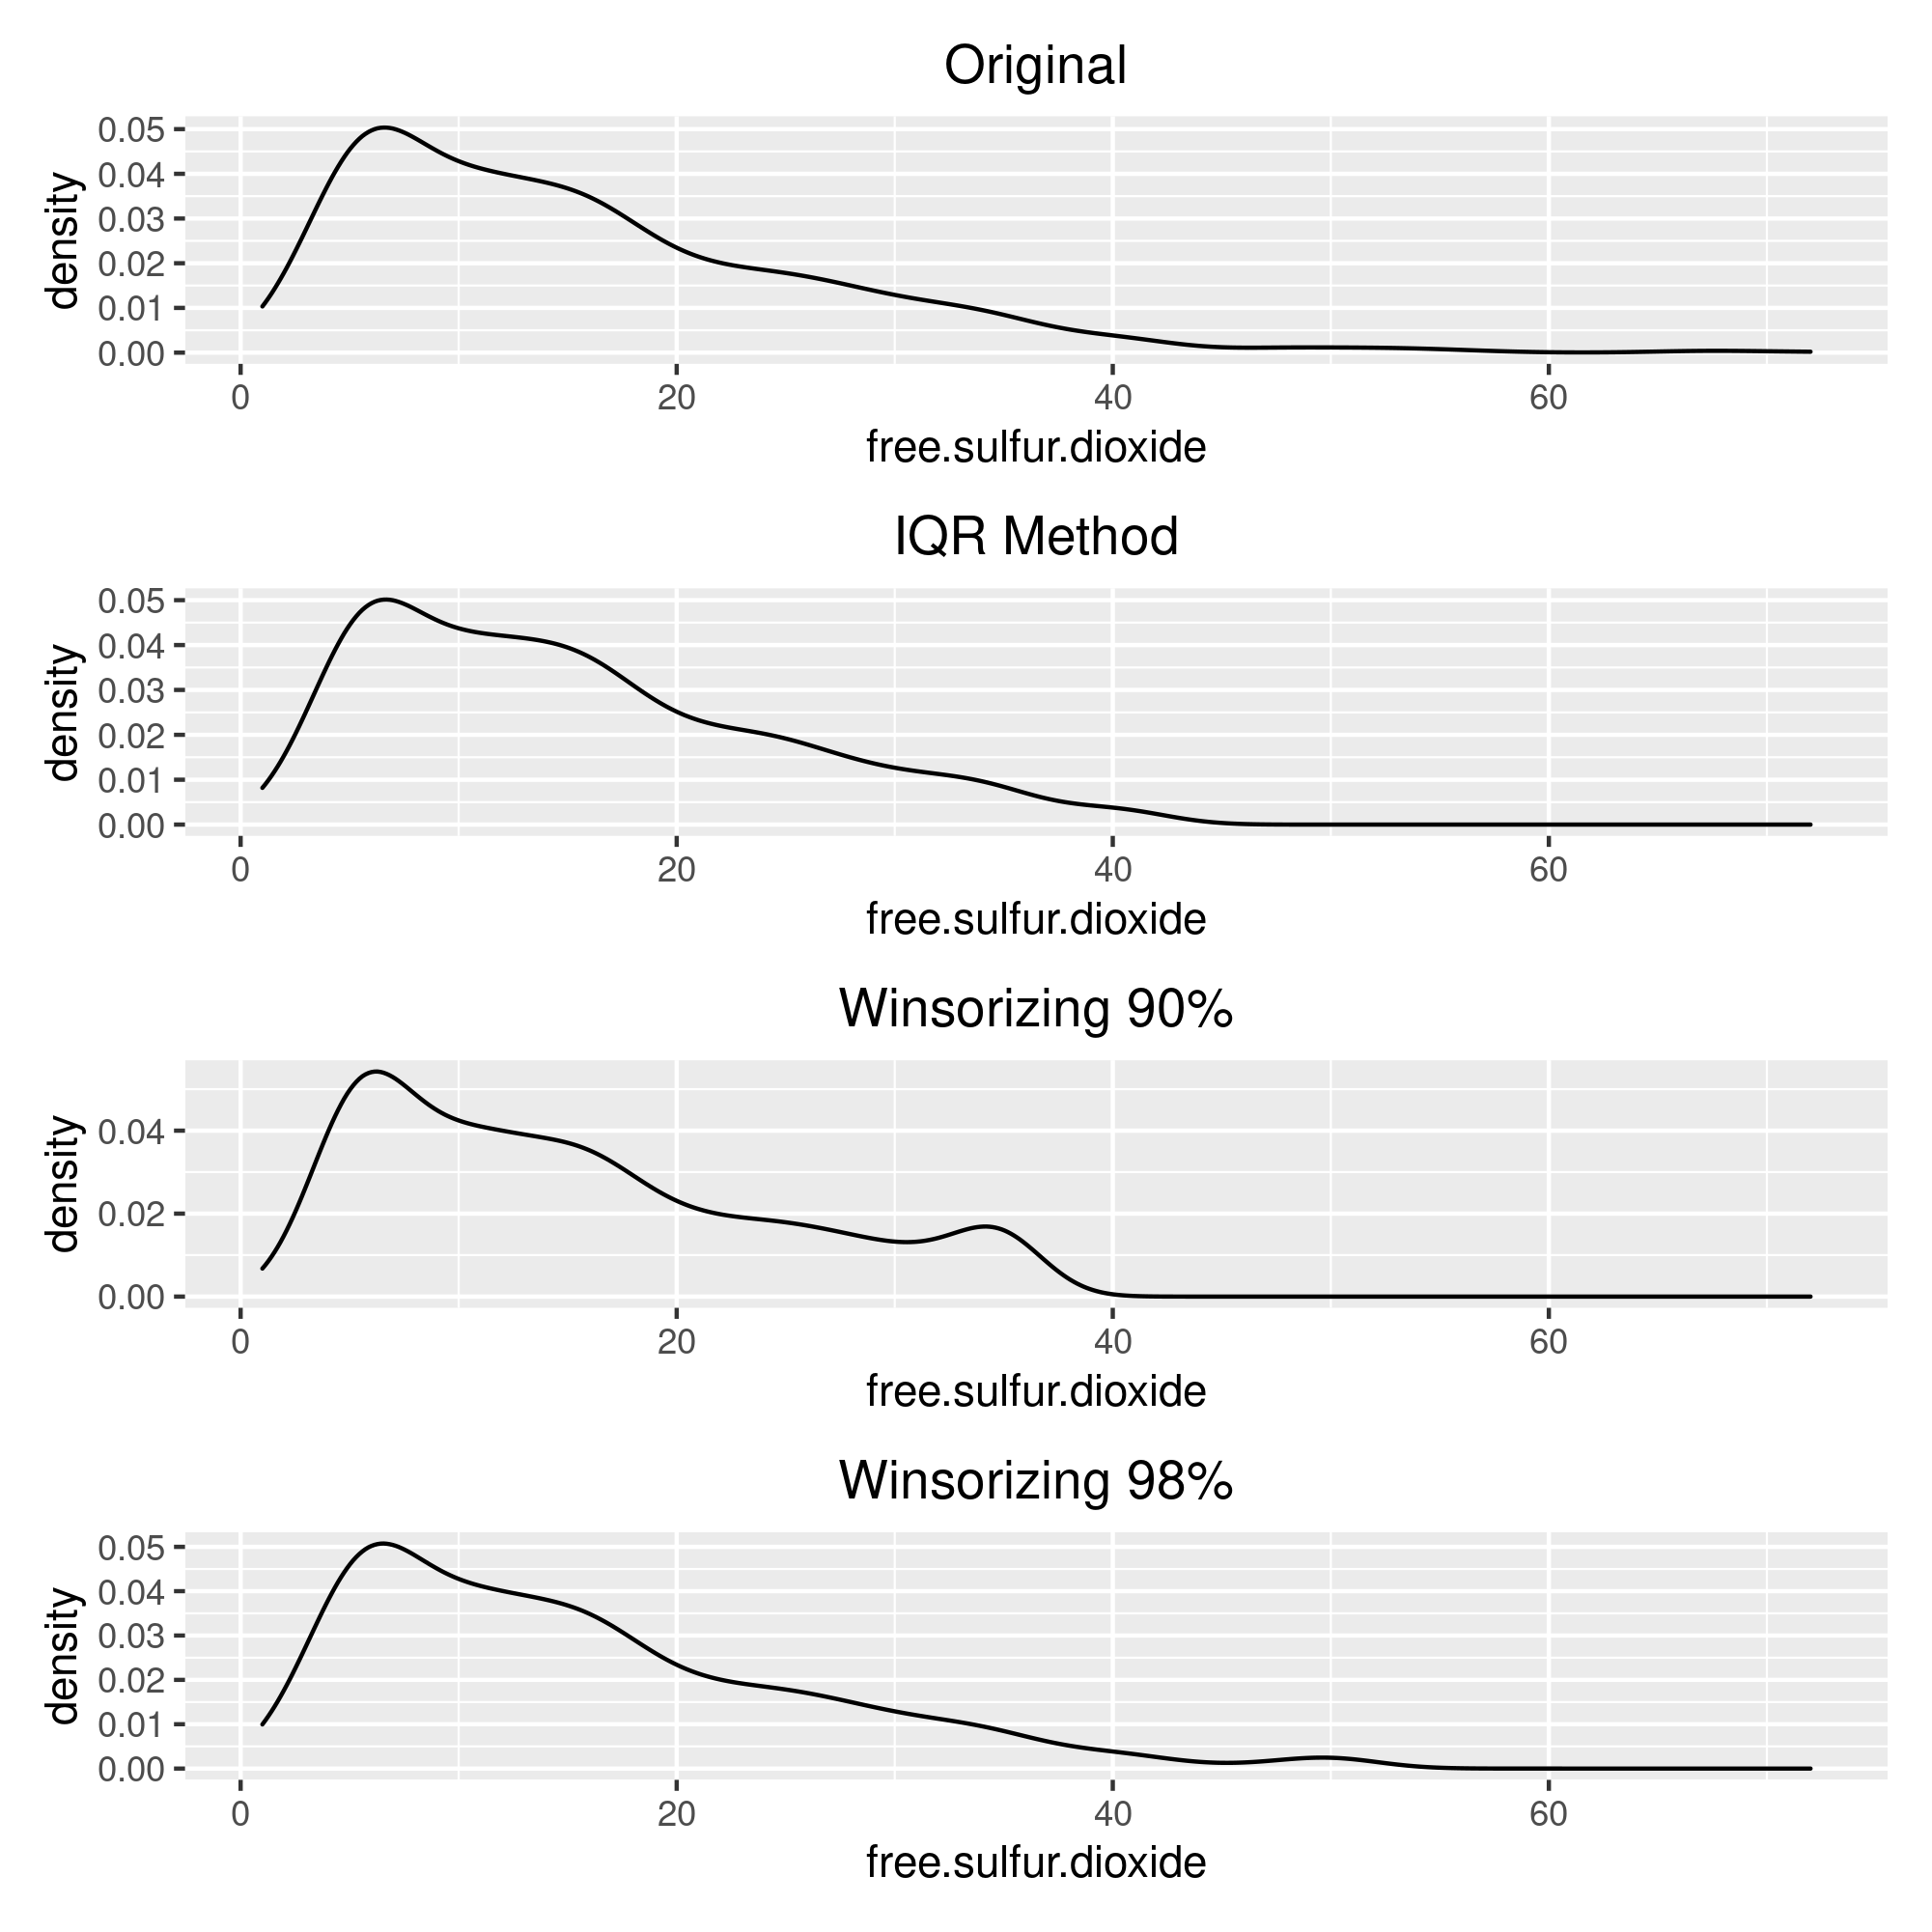
\includegraphics[width=0.45\textwidth]{images/outliers/free.sulfur.dioxide_distribution.png}
    }\qquad
    \subfloat[]{%
        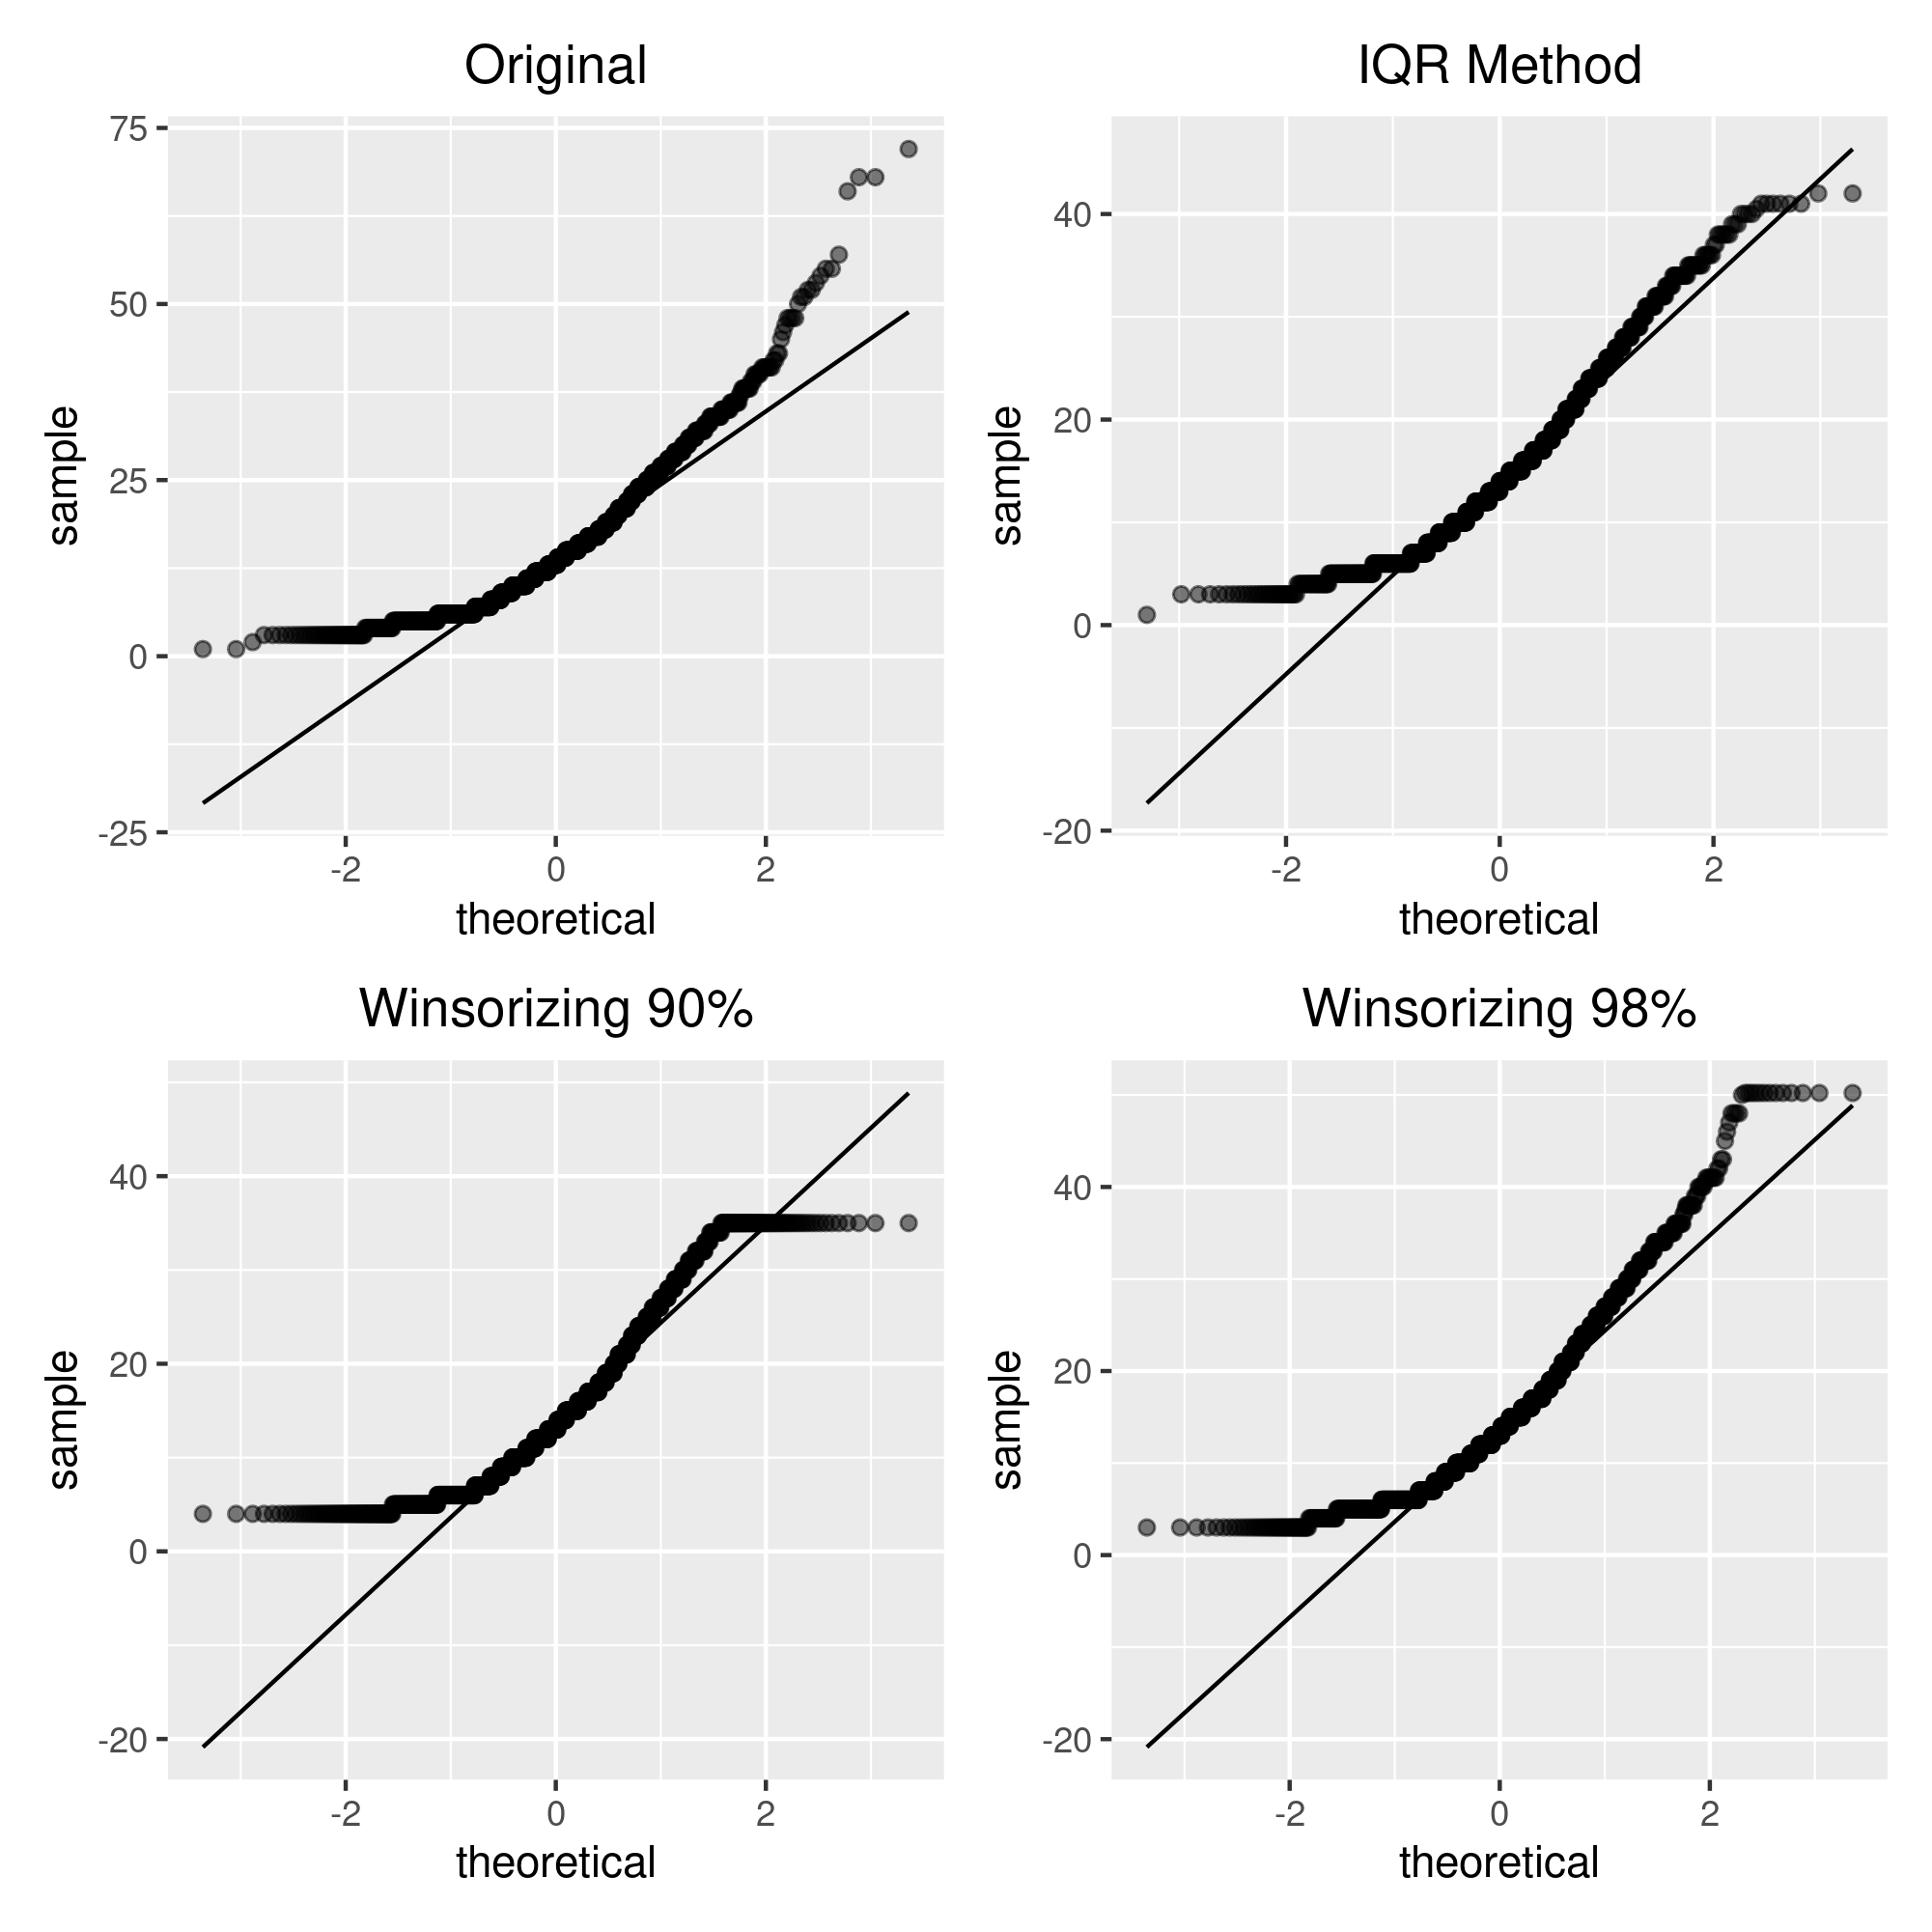
\includegraphics[width=0.45\textwidth]{images/outliers/free.sulfur.dioxide_qqplot.png}
    }

    \label{fig:free.sulfur.dioxide}
    \caption{Commento}
\end{figure}

\begin{figure}[H]
    \centering

    \subfloat[]{%
        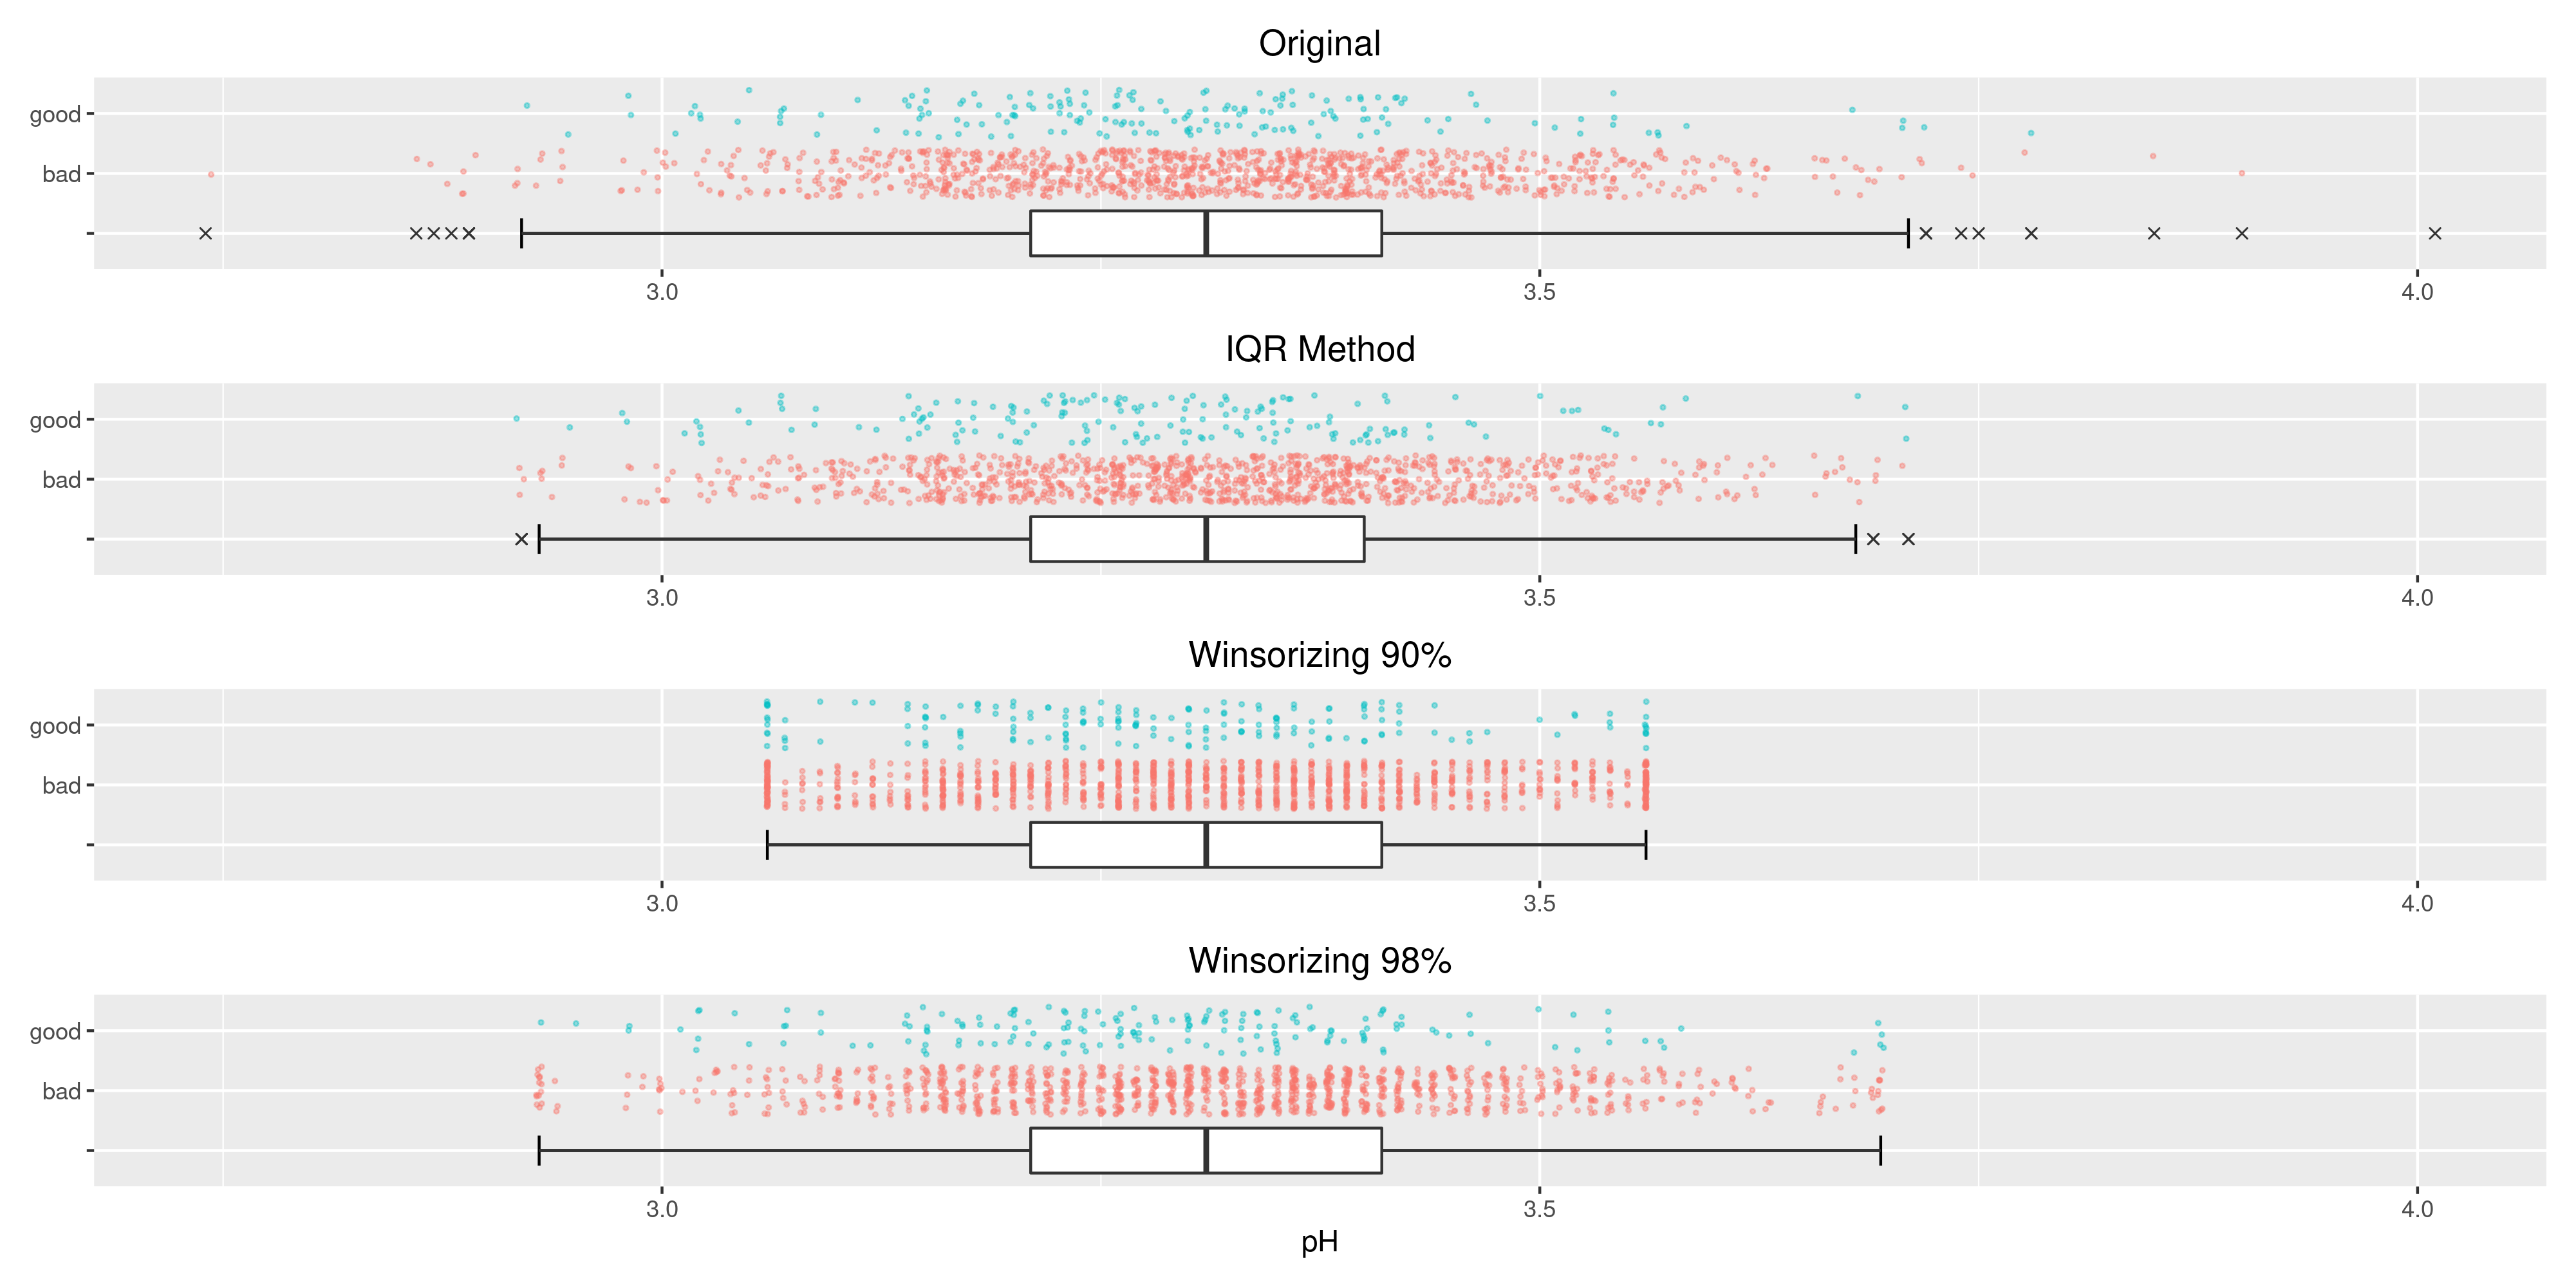
\includegraphics[width=0.99\textwidth]{images/outliers/pH_boxplot.png}
    }

    \subfloat[]{%
        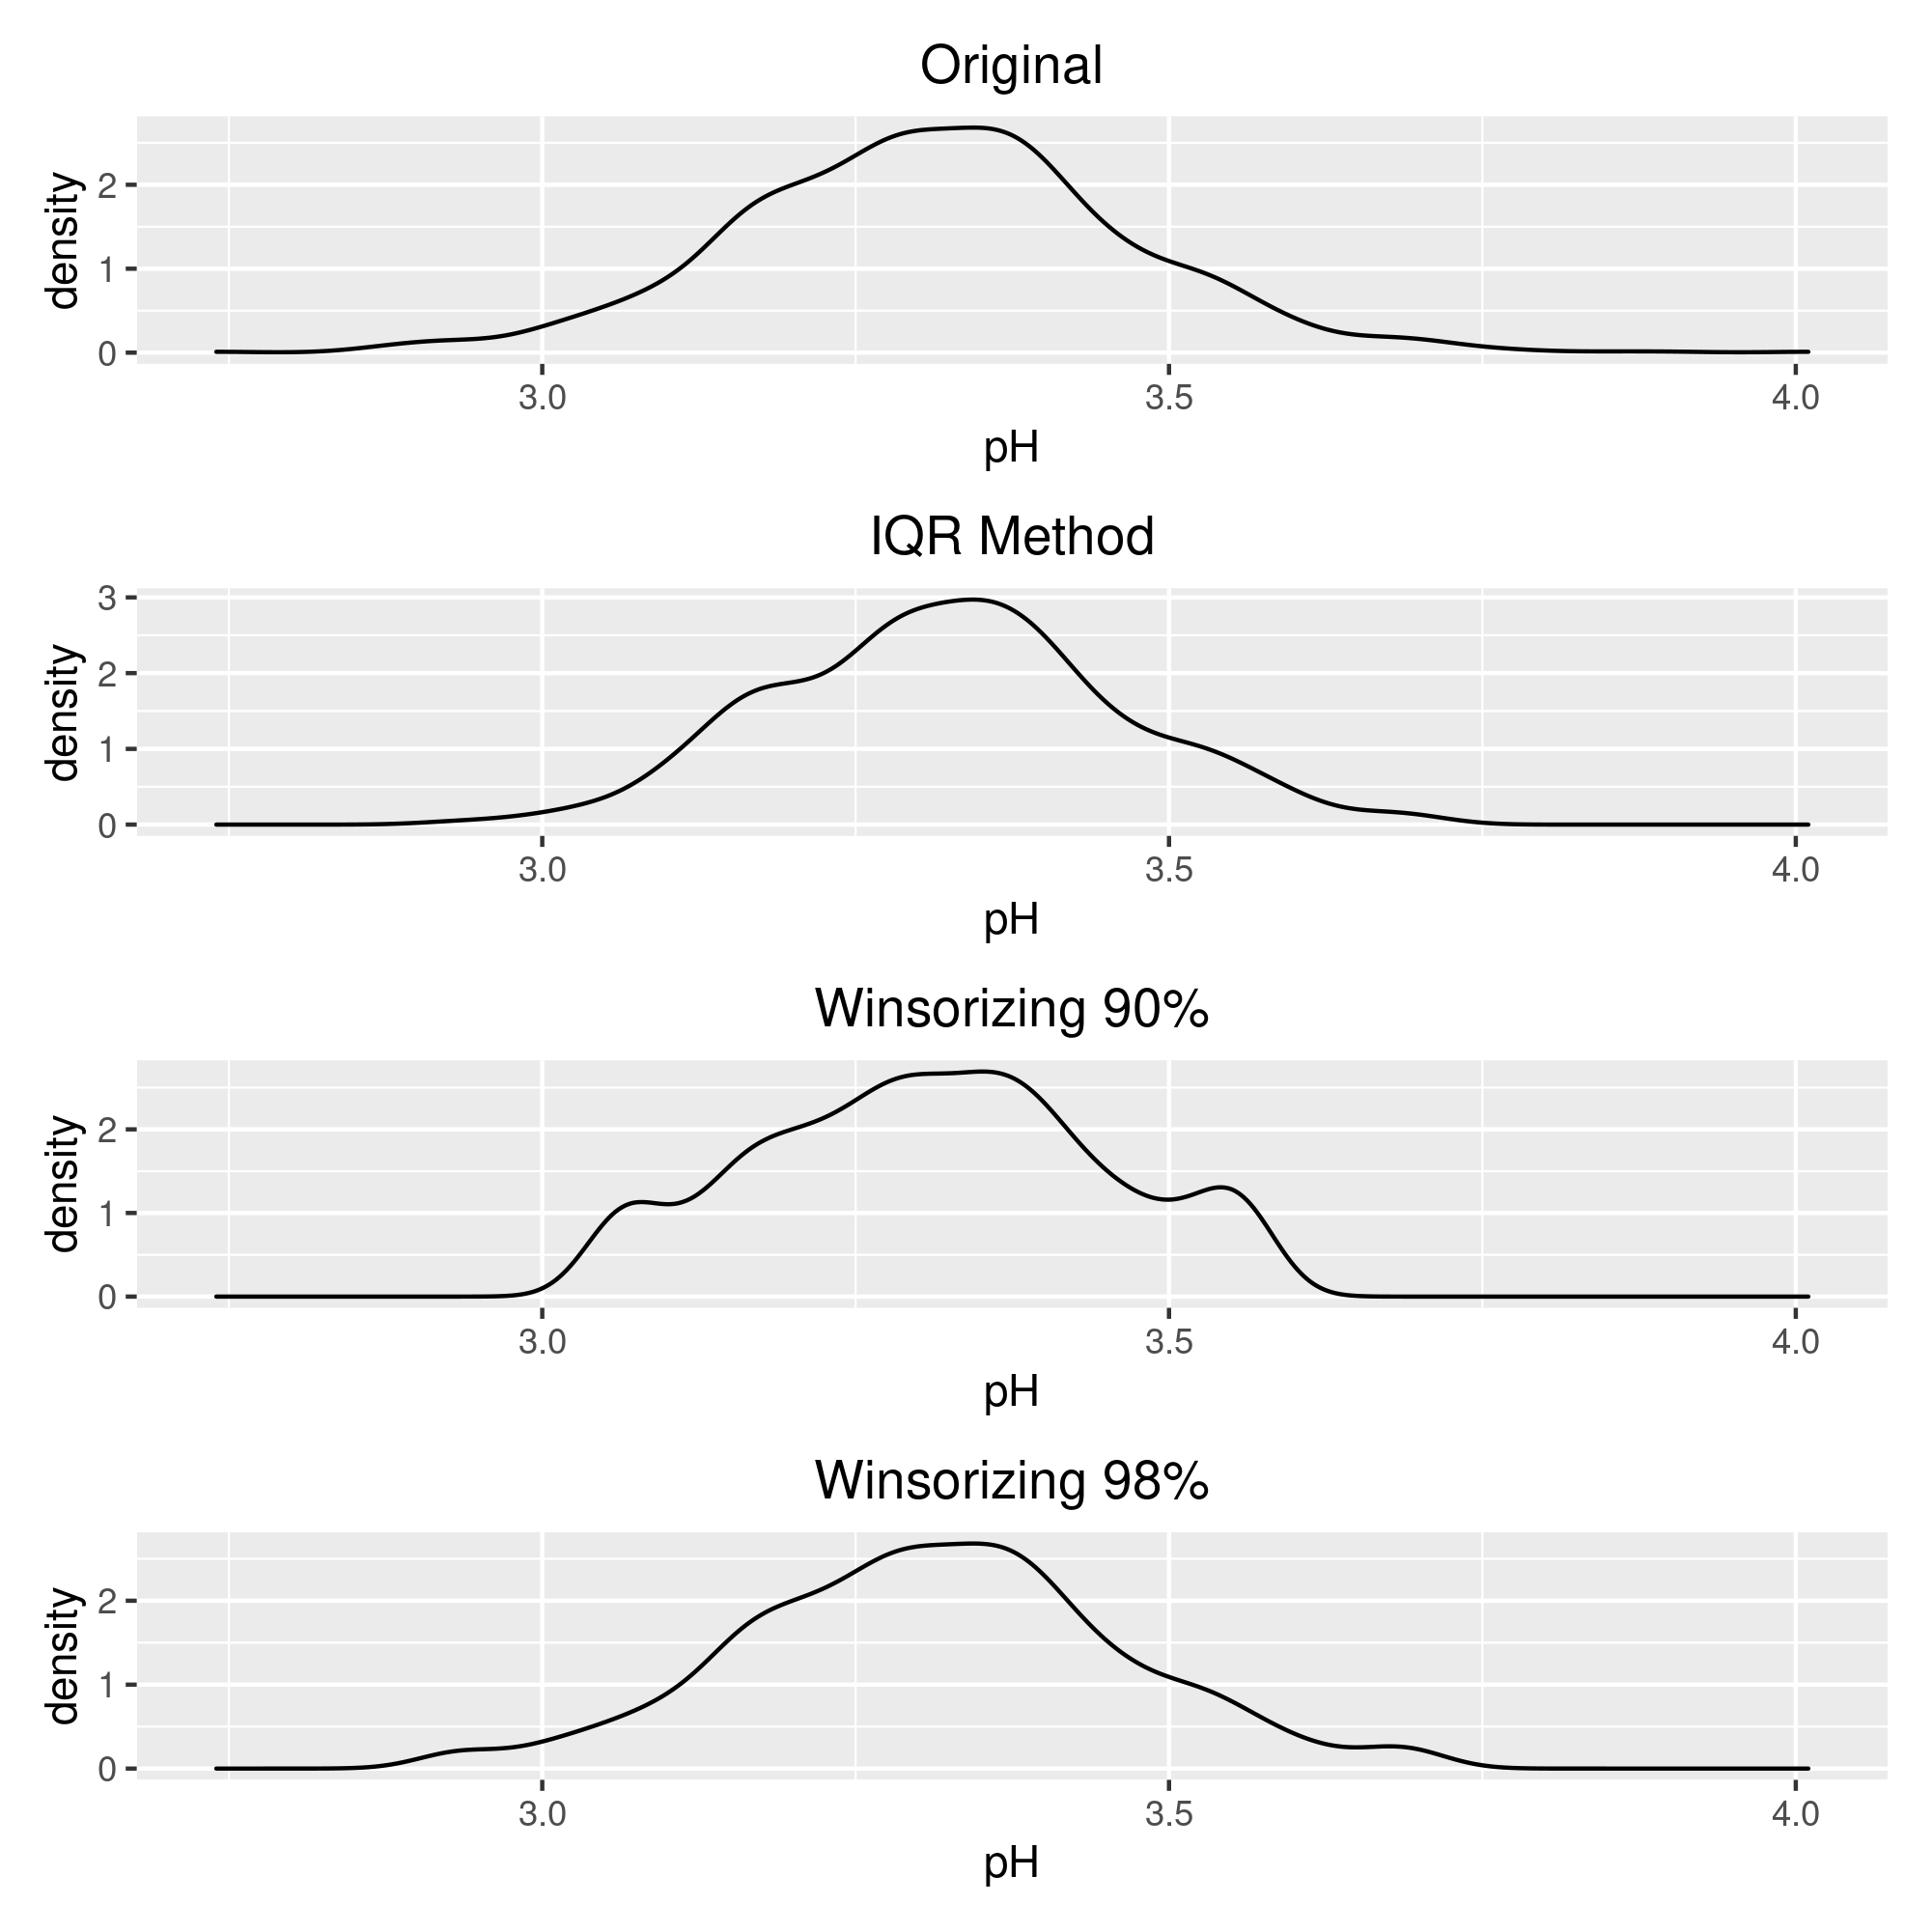
\includegraphics[width=0.45\textwidth]{images/outliers/pH_distribution.png}
    }\qquad
    \subfloat[]{%
        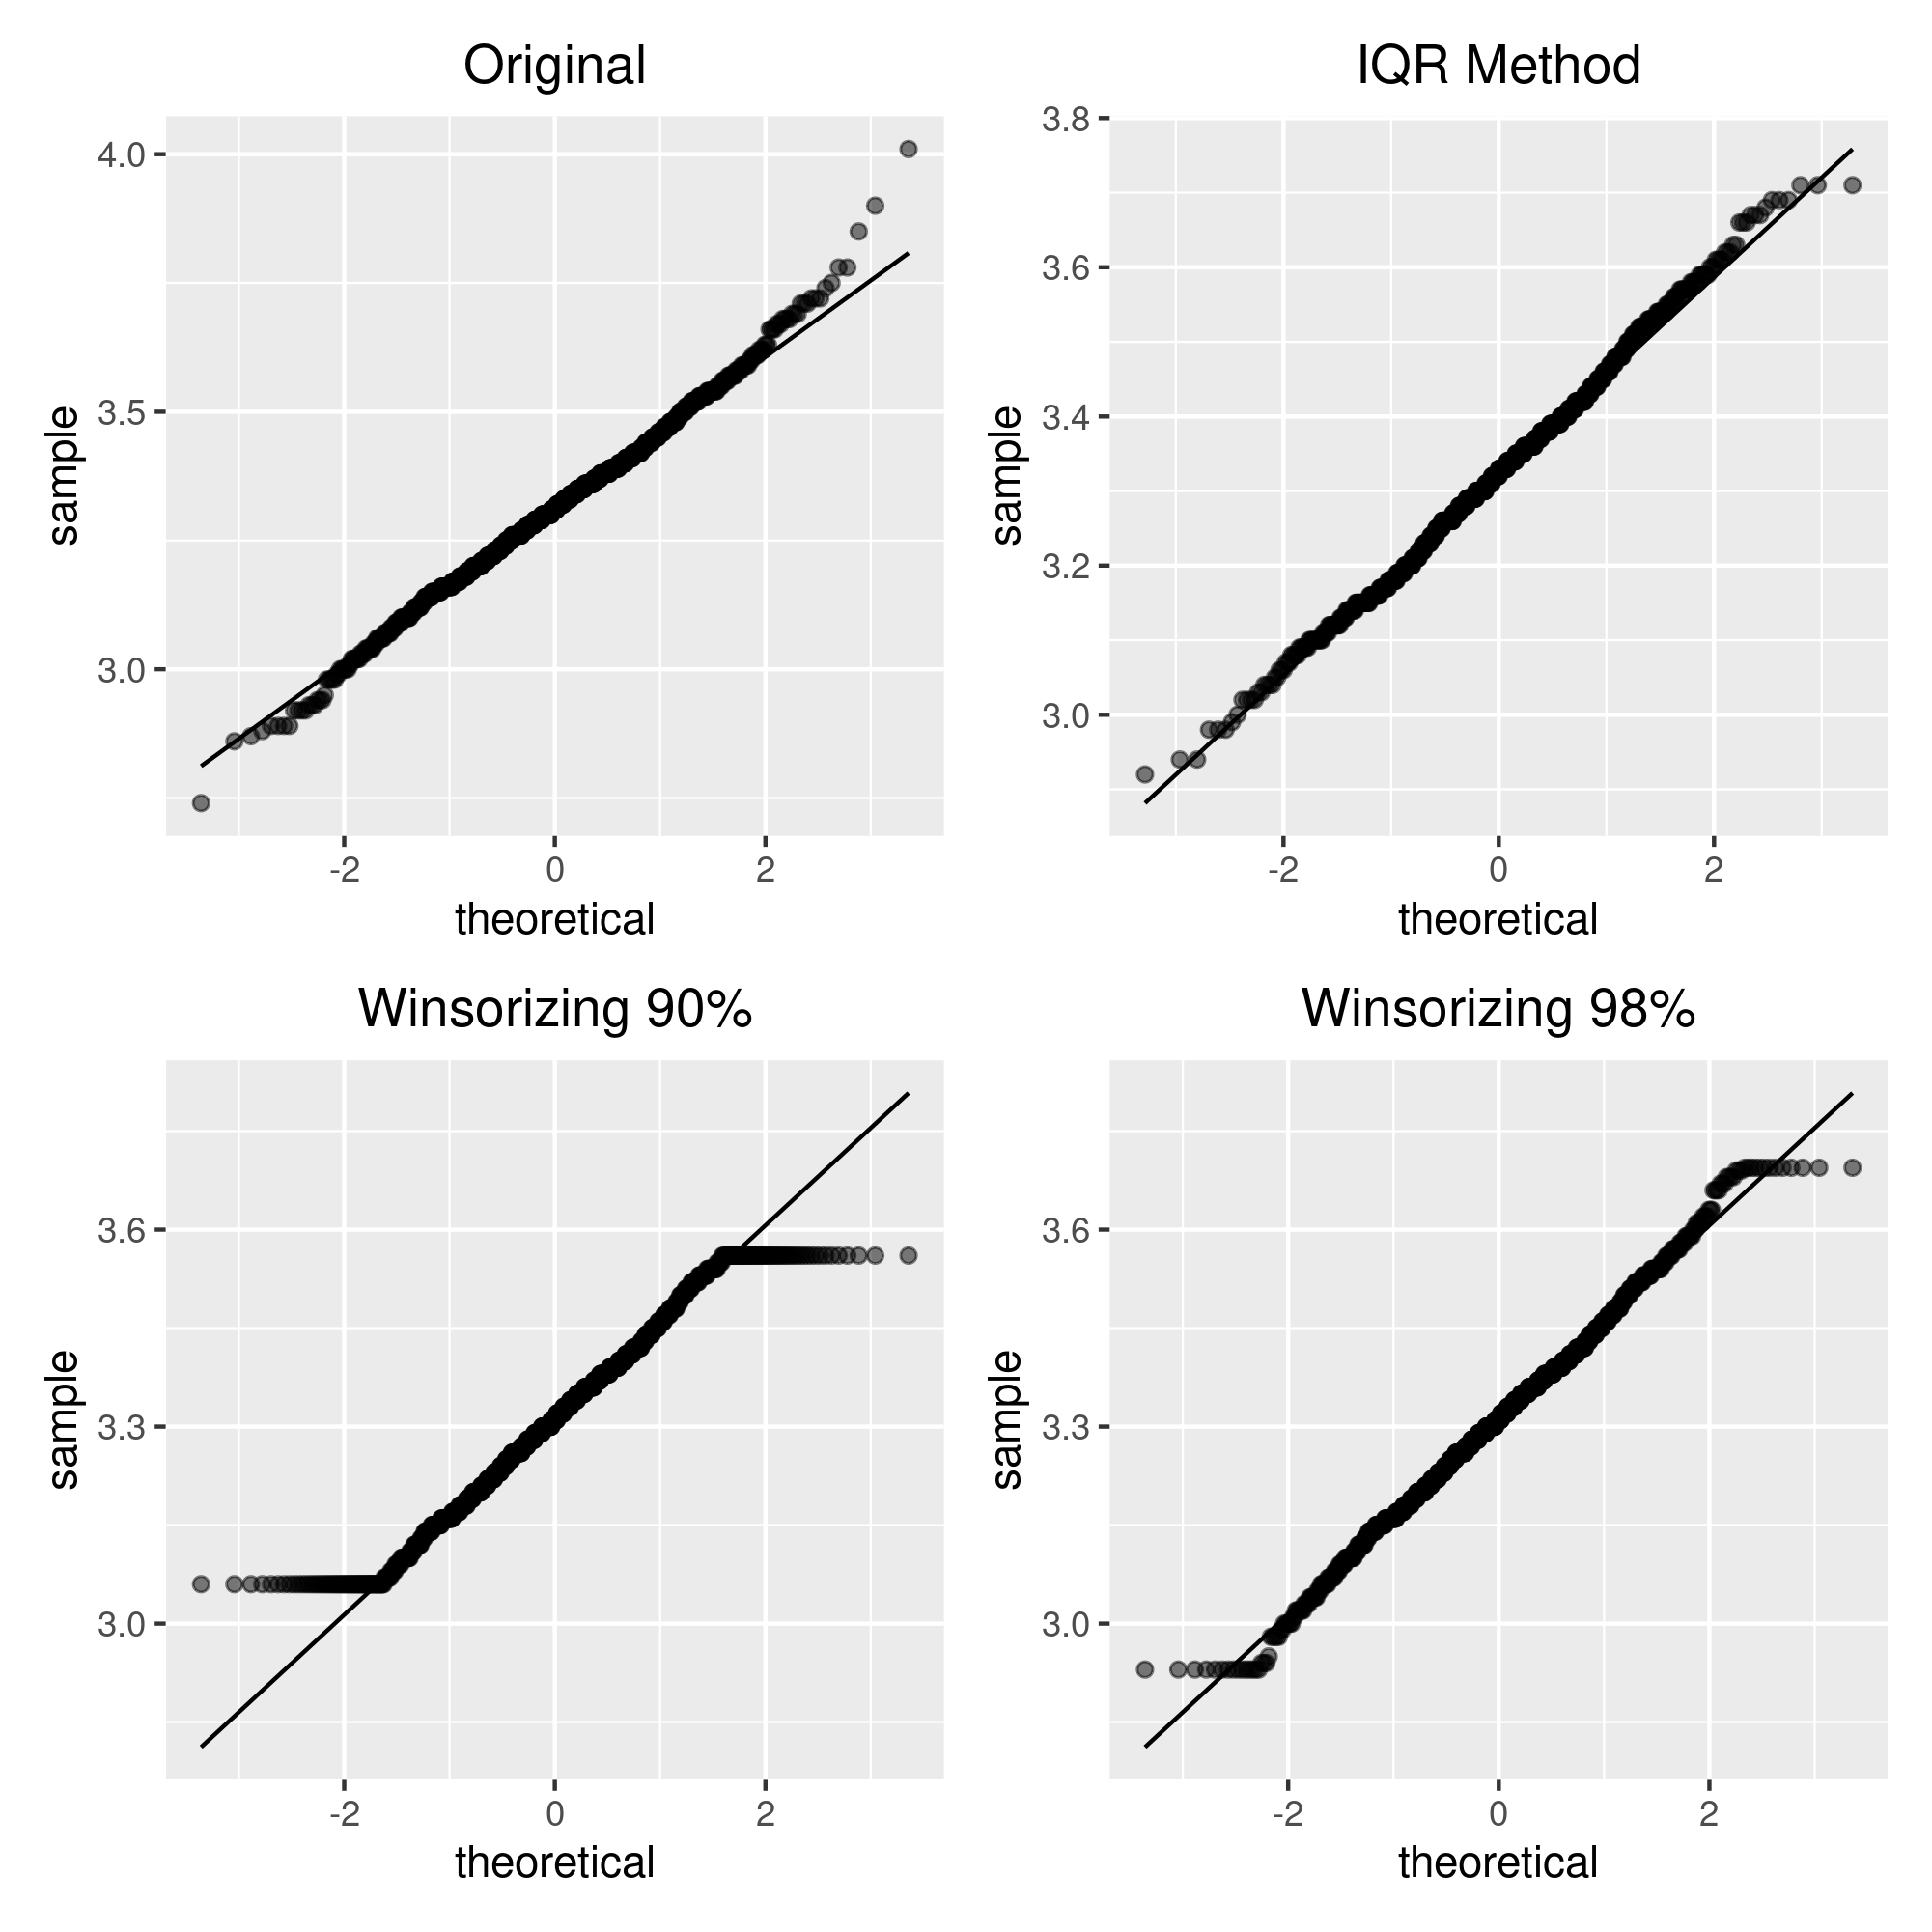
\includegraphics[width=0.45\textwidth]{images/outliers/pH_qqplot.png}
    }

    \label{fig:pH}
    \caption{Commento}
\end{figure}

\begin{figure}[H]
    \centering

    \subfloat[]{%
        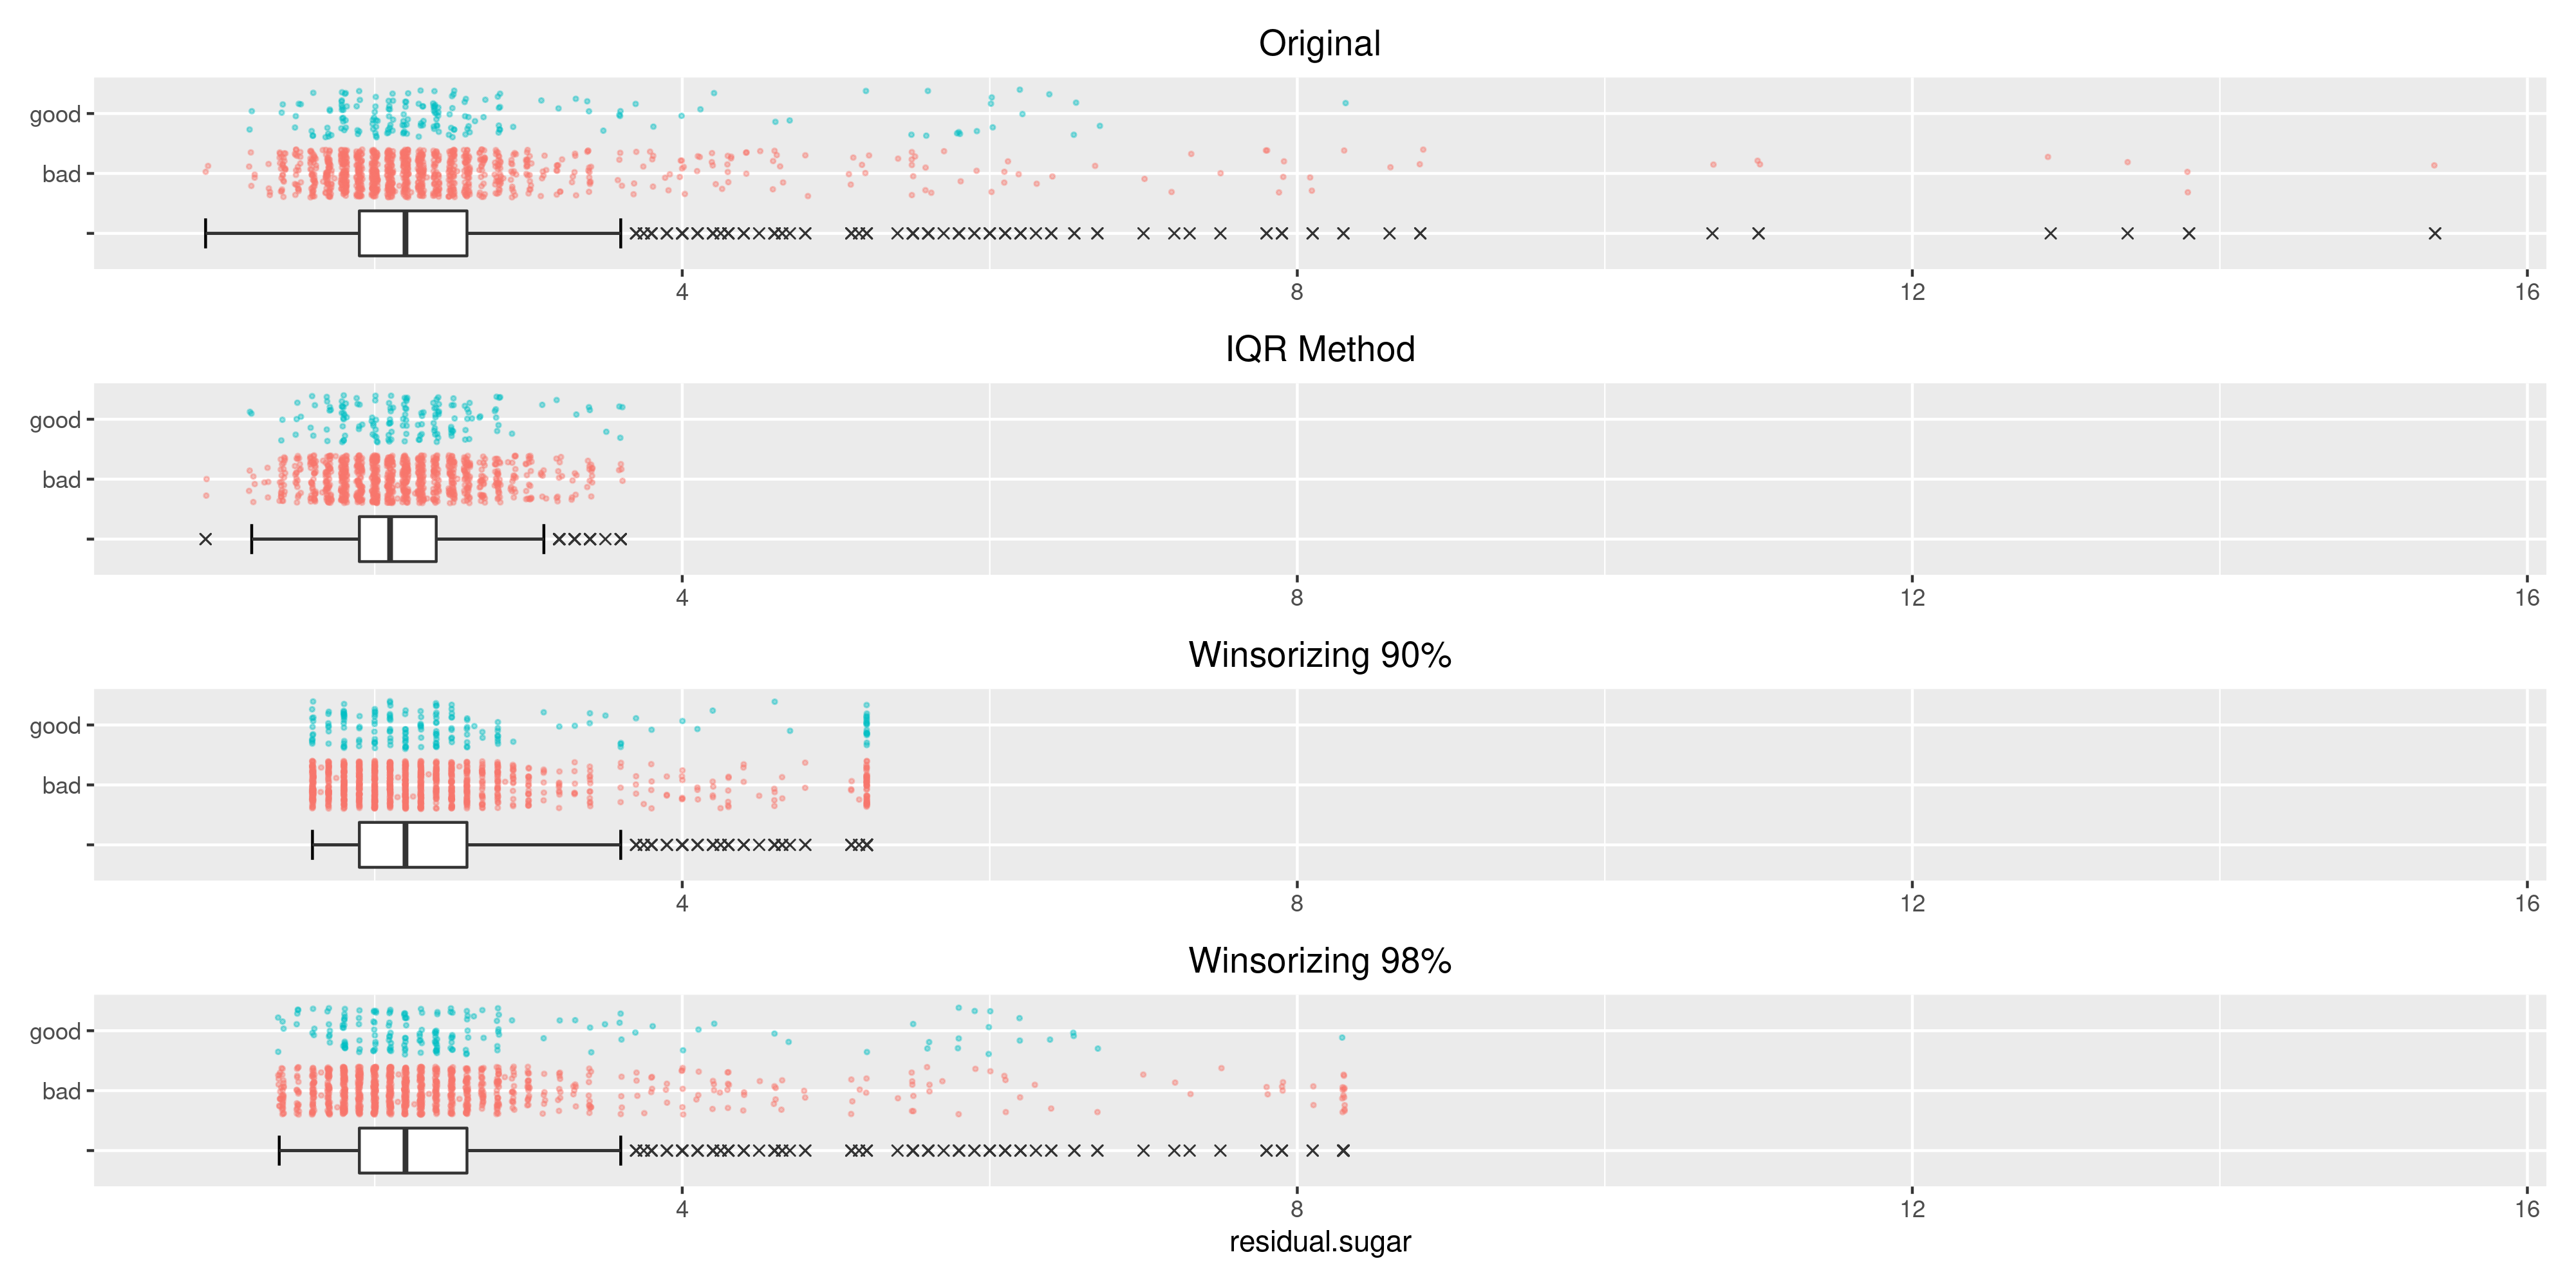
\includegraphics[width=0.99\textwidth]{images/outliers/residual.sugar_boxplot.png}
    }

    \subfloat[]{%
        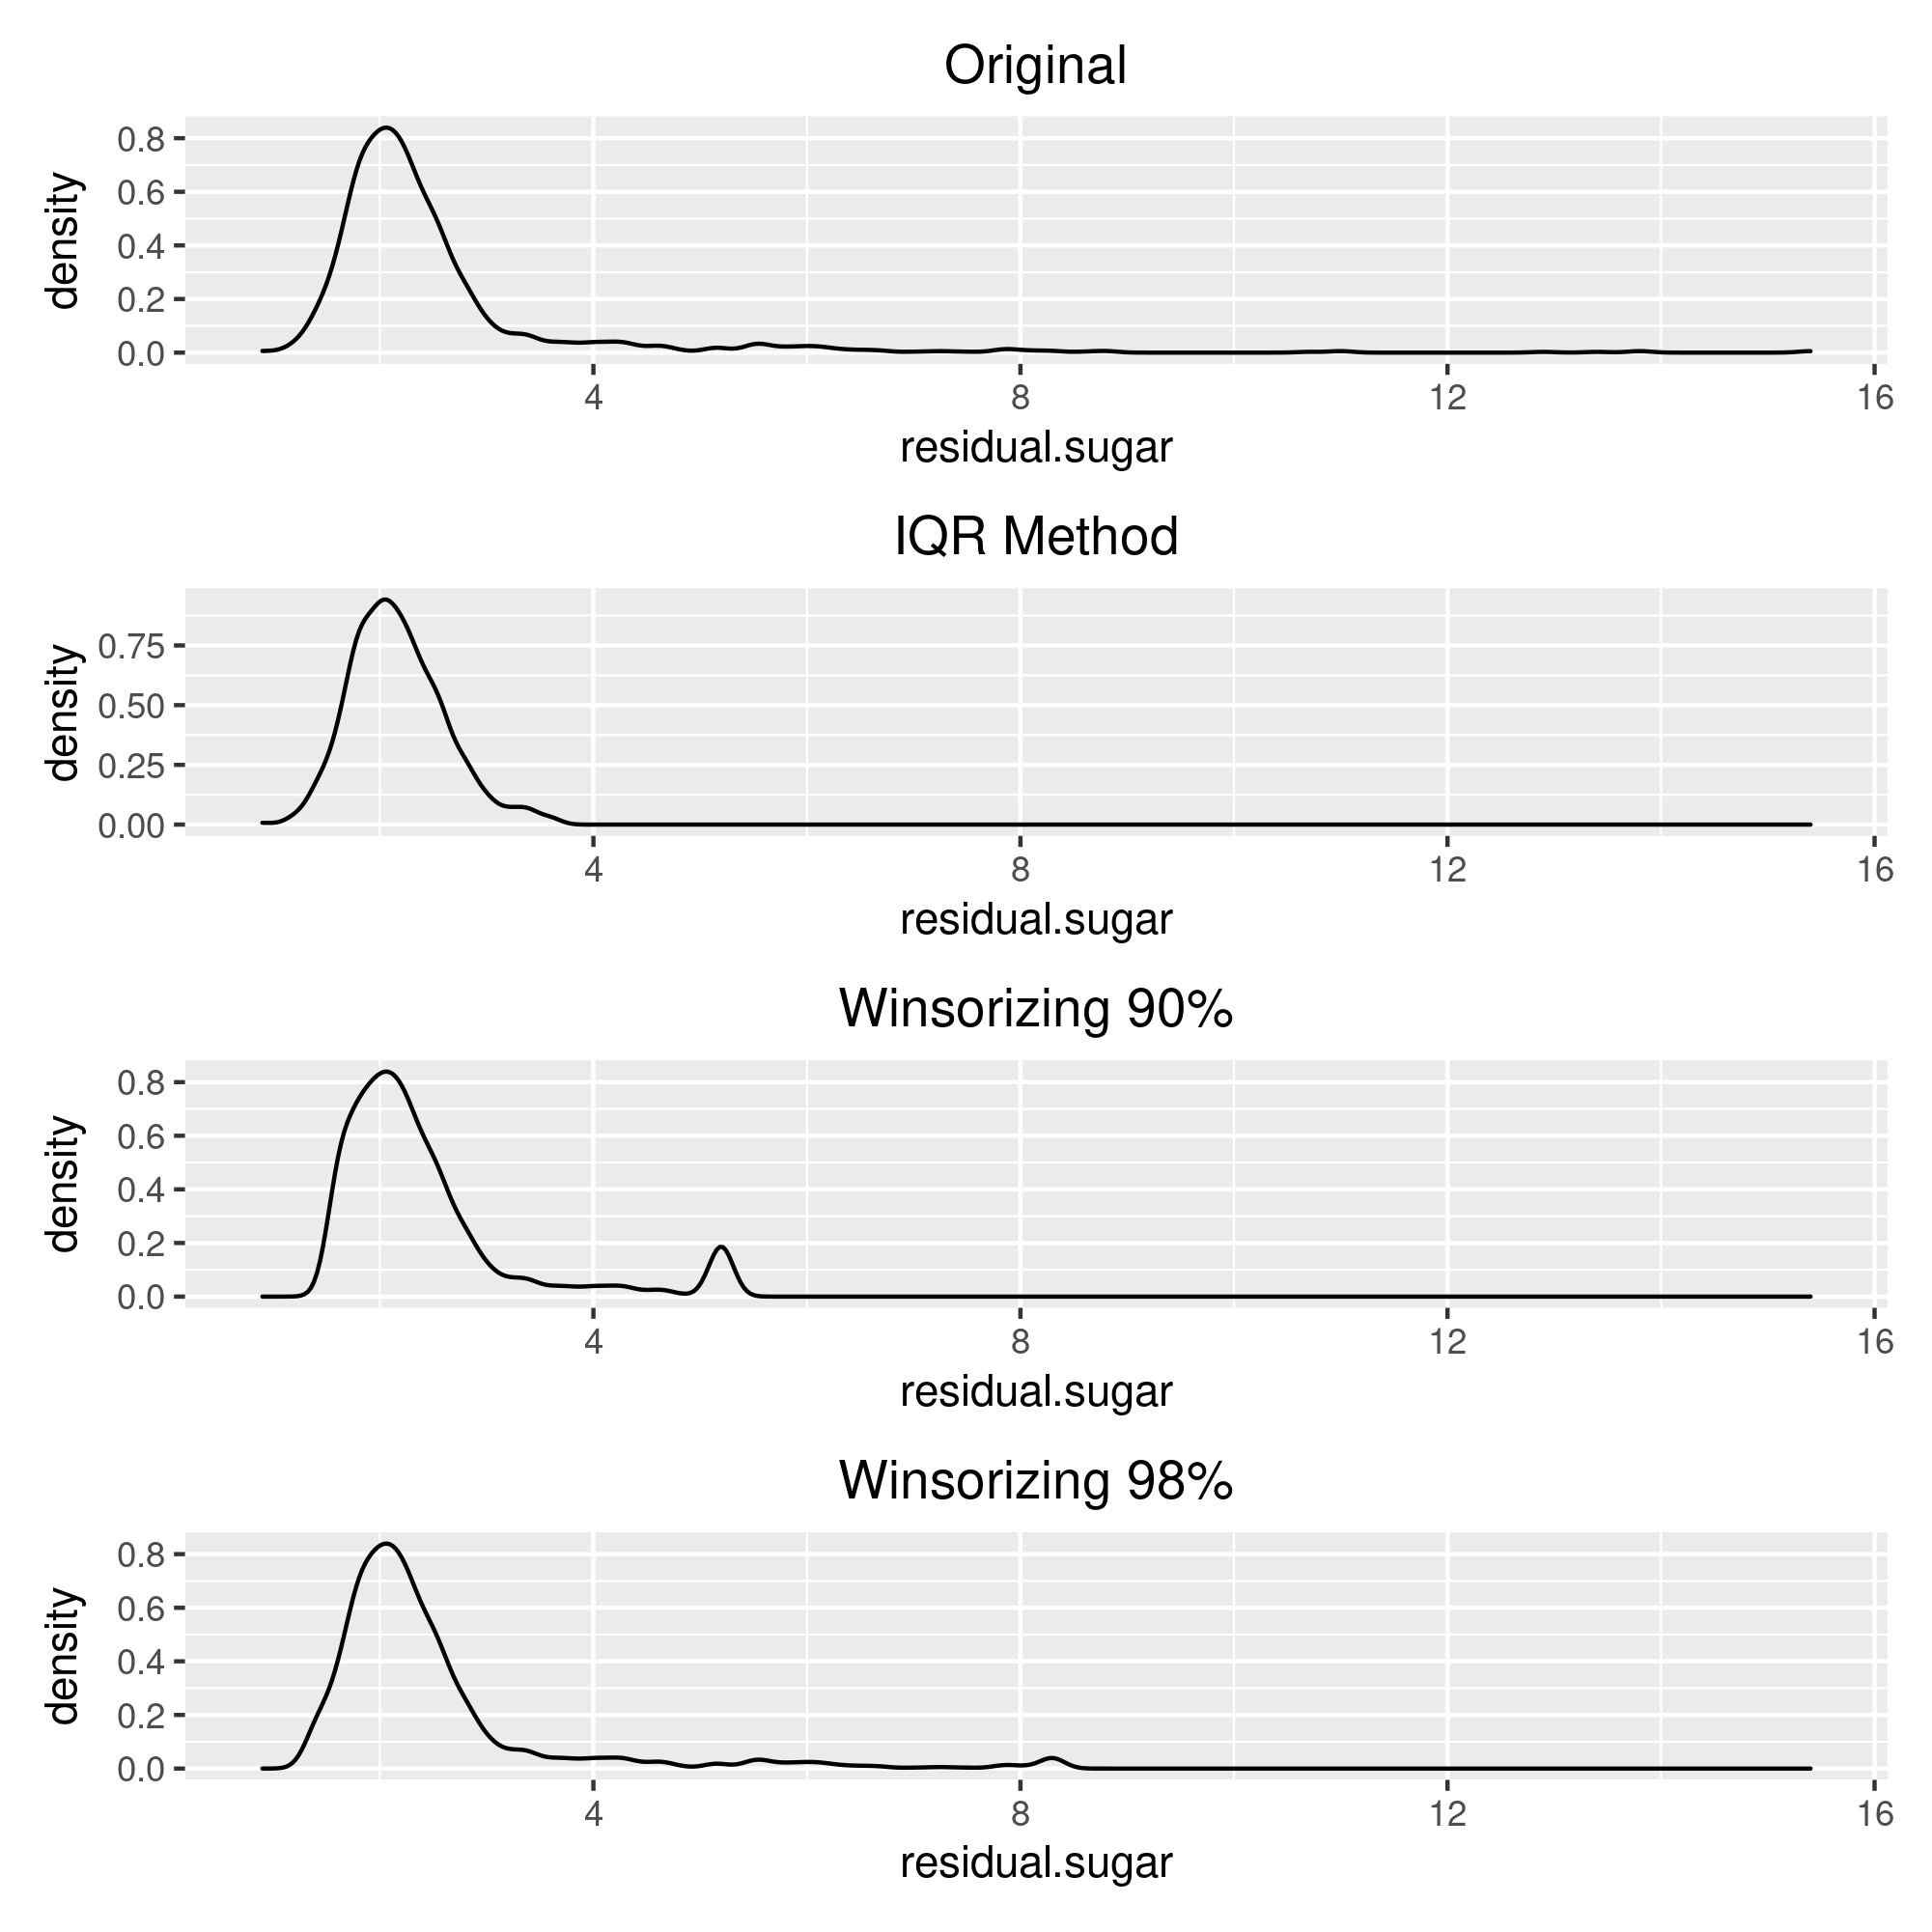
\includegraphics[width=0.45\textwidth]{images/outliers/residual.sugar_distribution.png}
    }\qquad
    \subfloat[]{%
        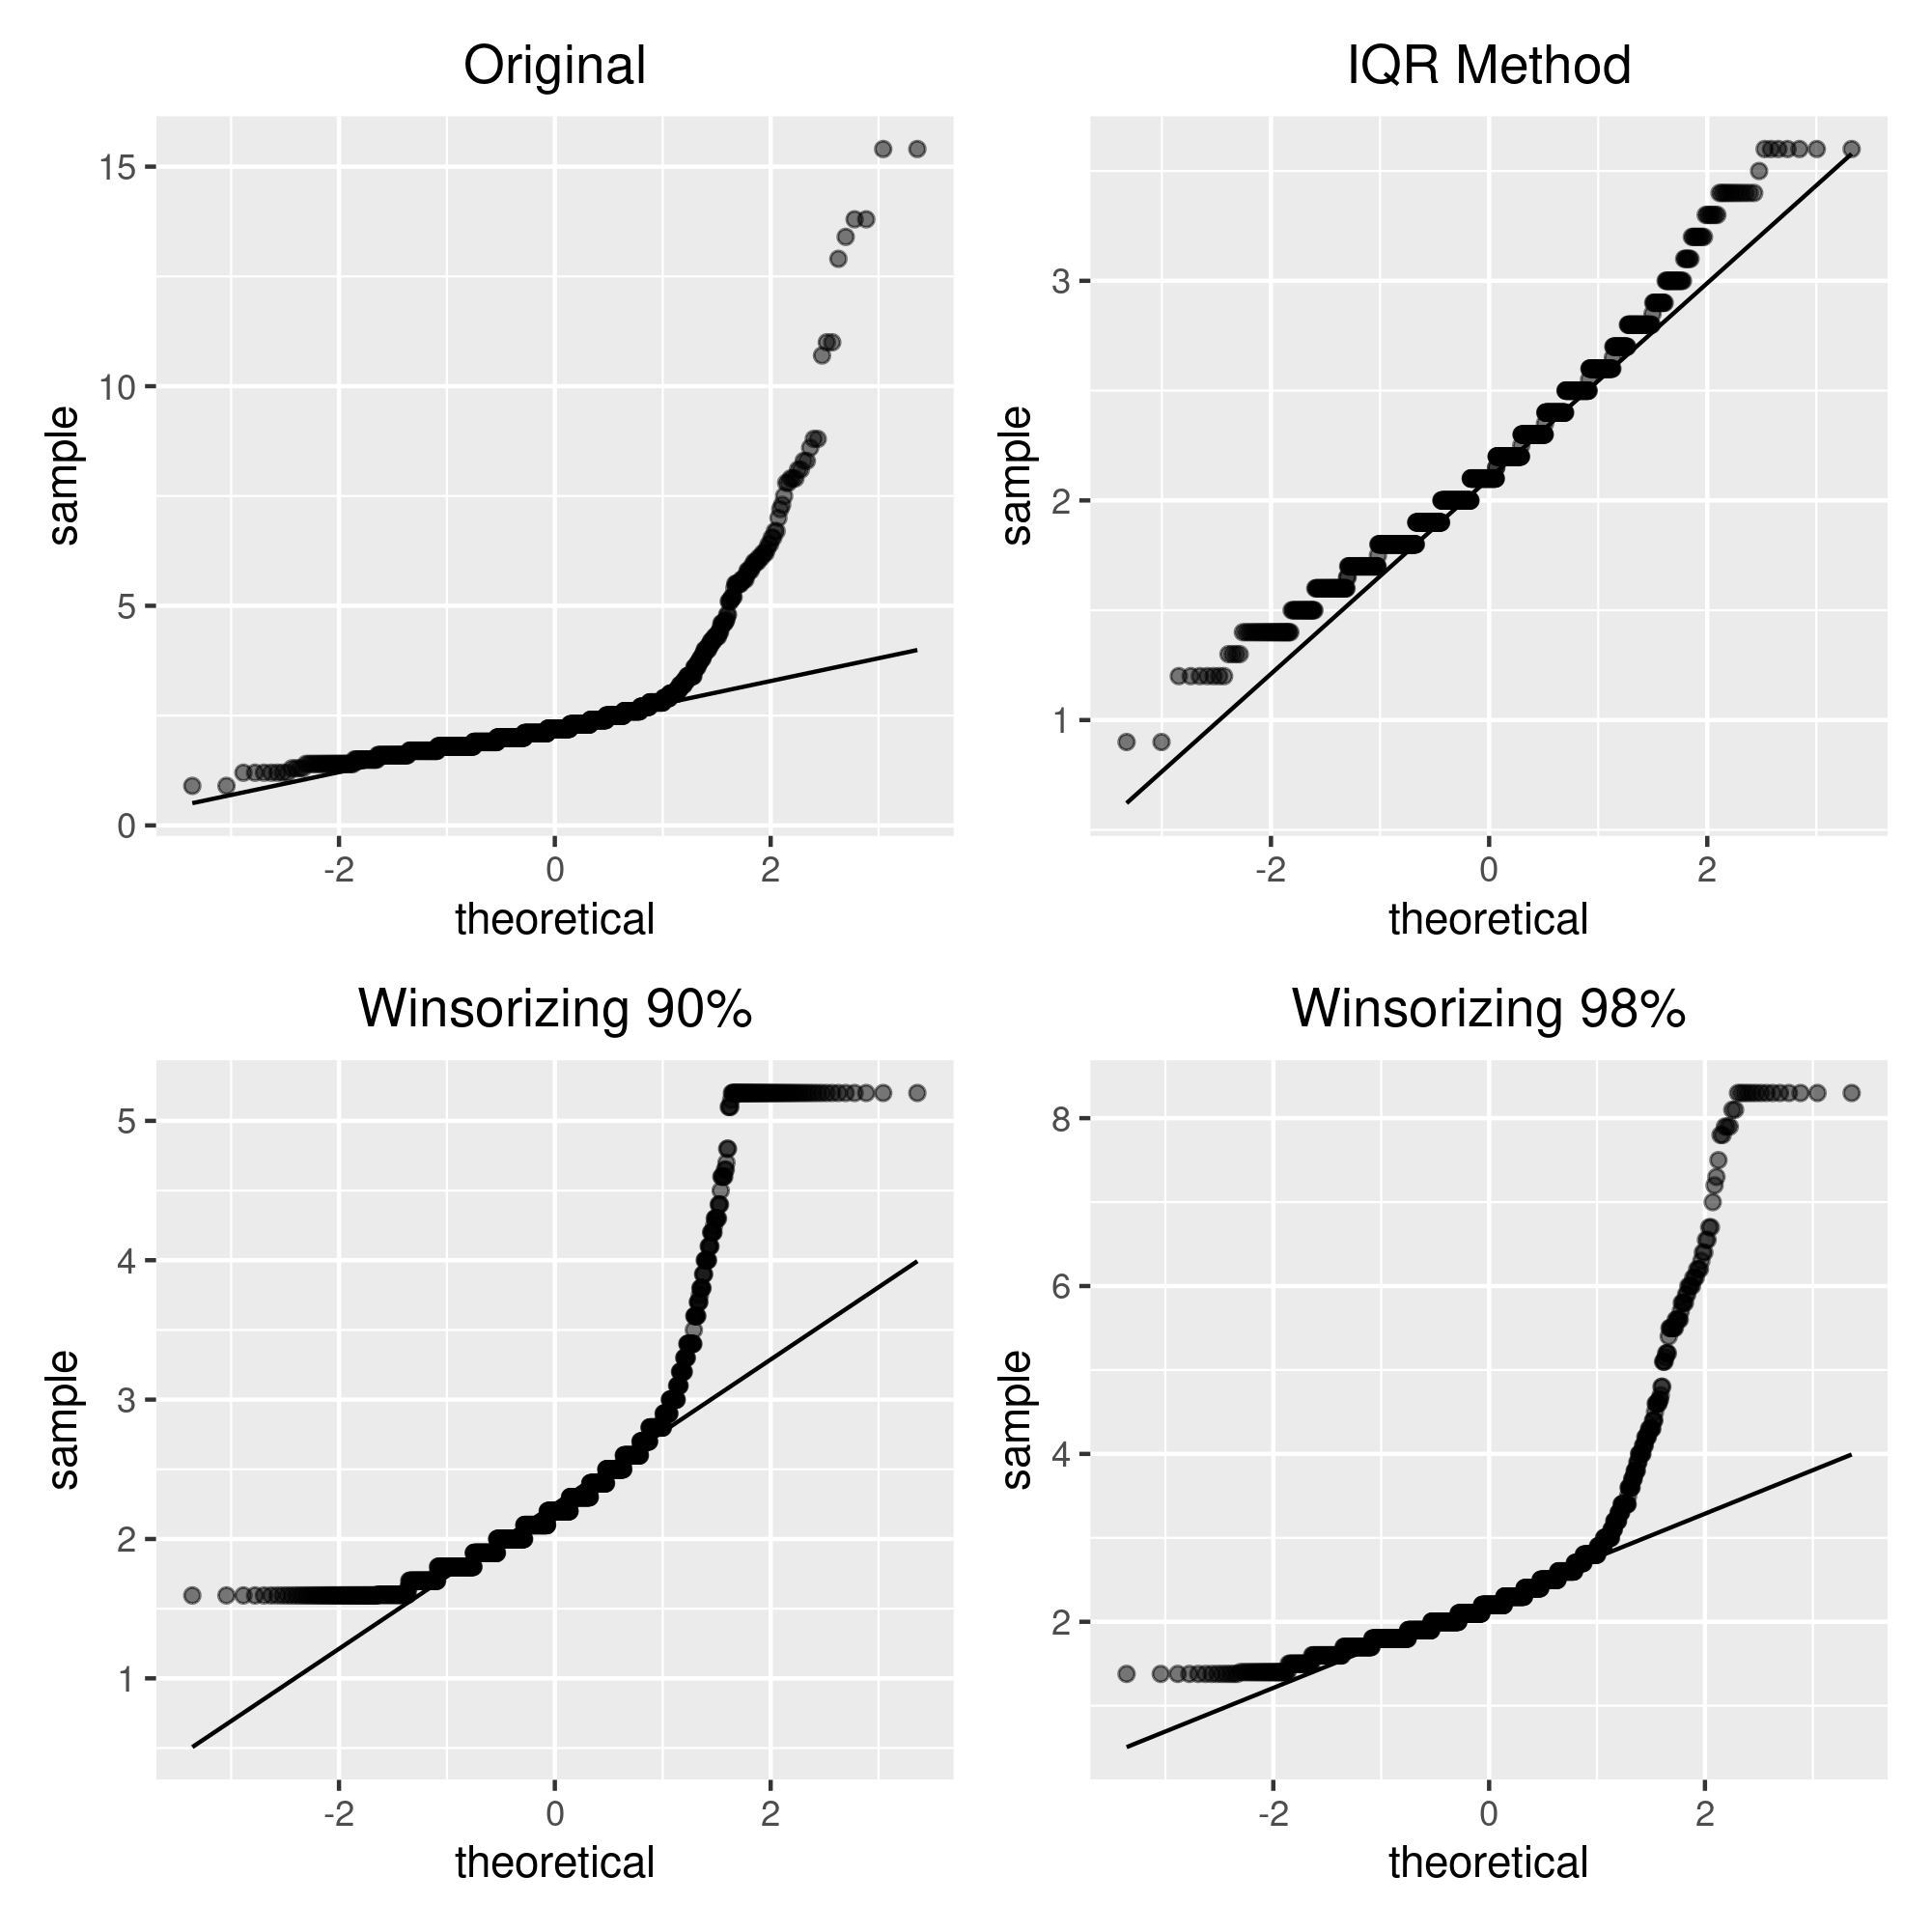
\includegraphics[width=0.45\textwidth]{images/outliers/residual.sugar_qqplot.png}
    }

    \label{fig:residual.sugar}
    \caption{Commento}
\end{figure}

\begin{figure}[H]
    \centering

    \subfloat[]{%
        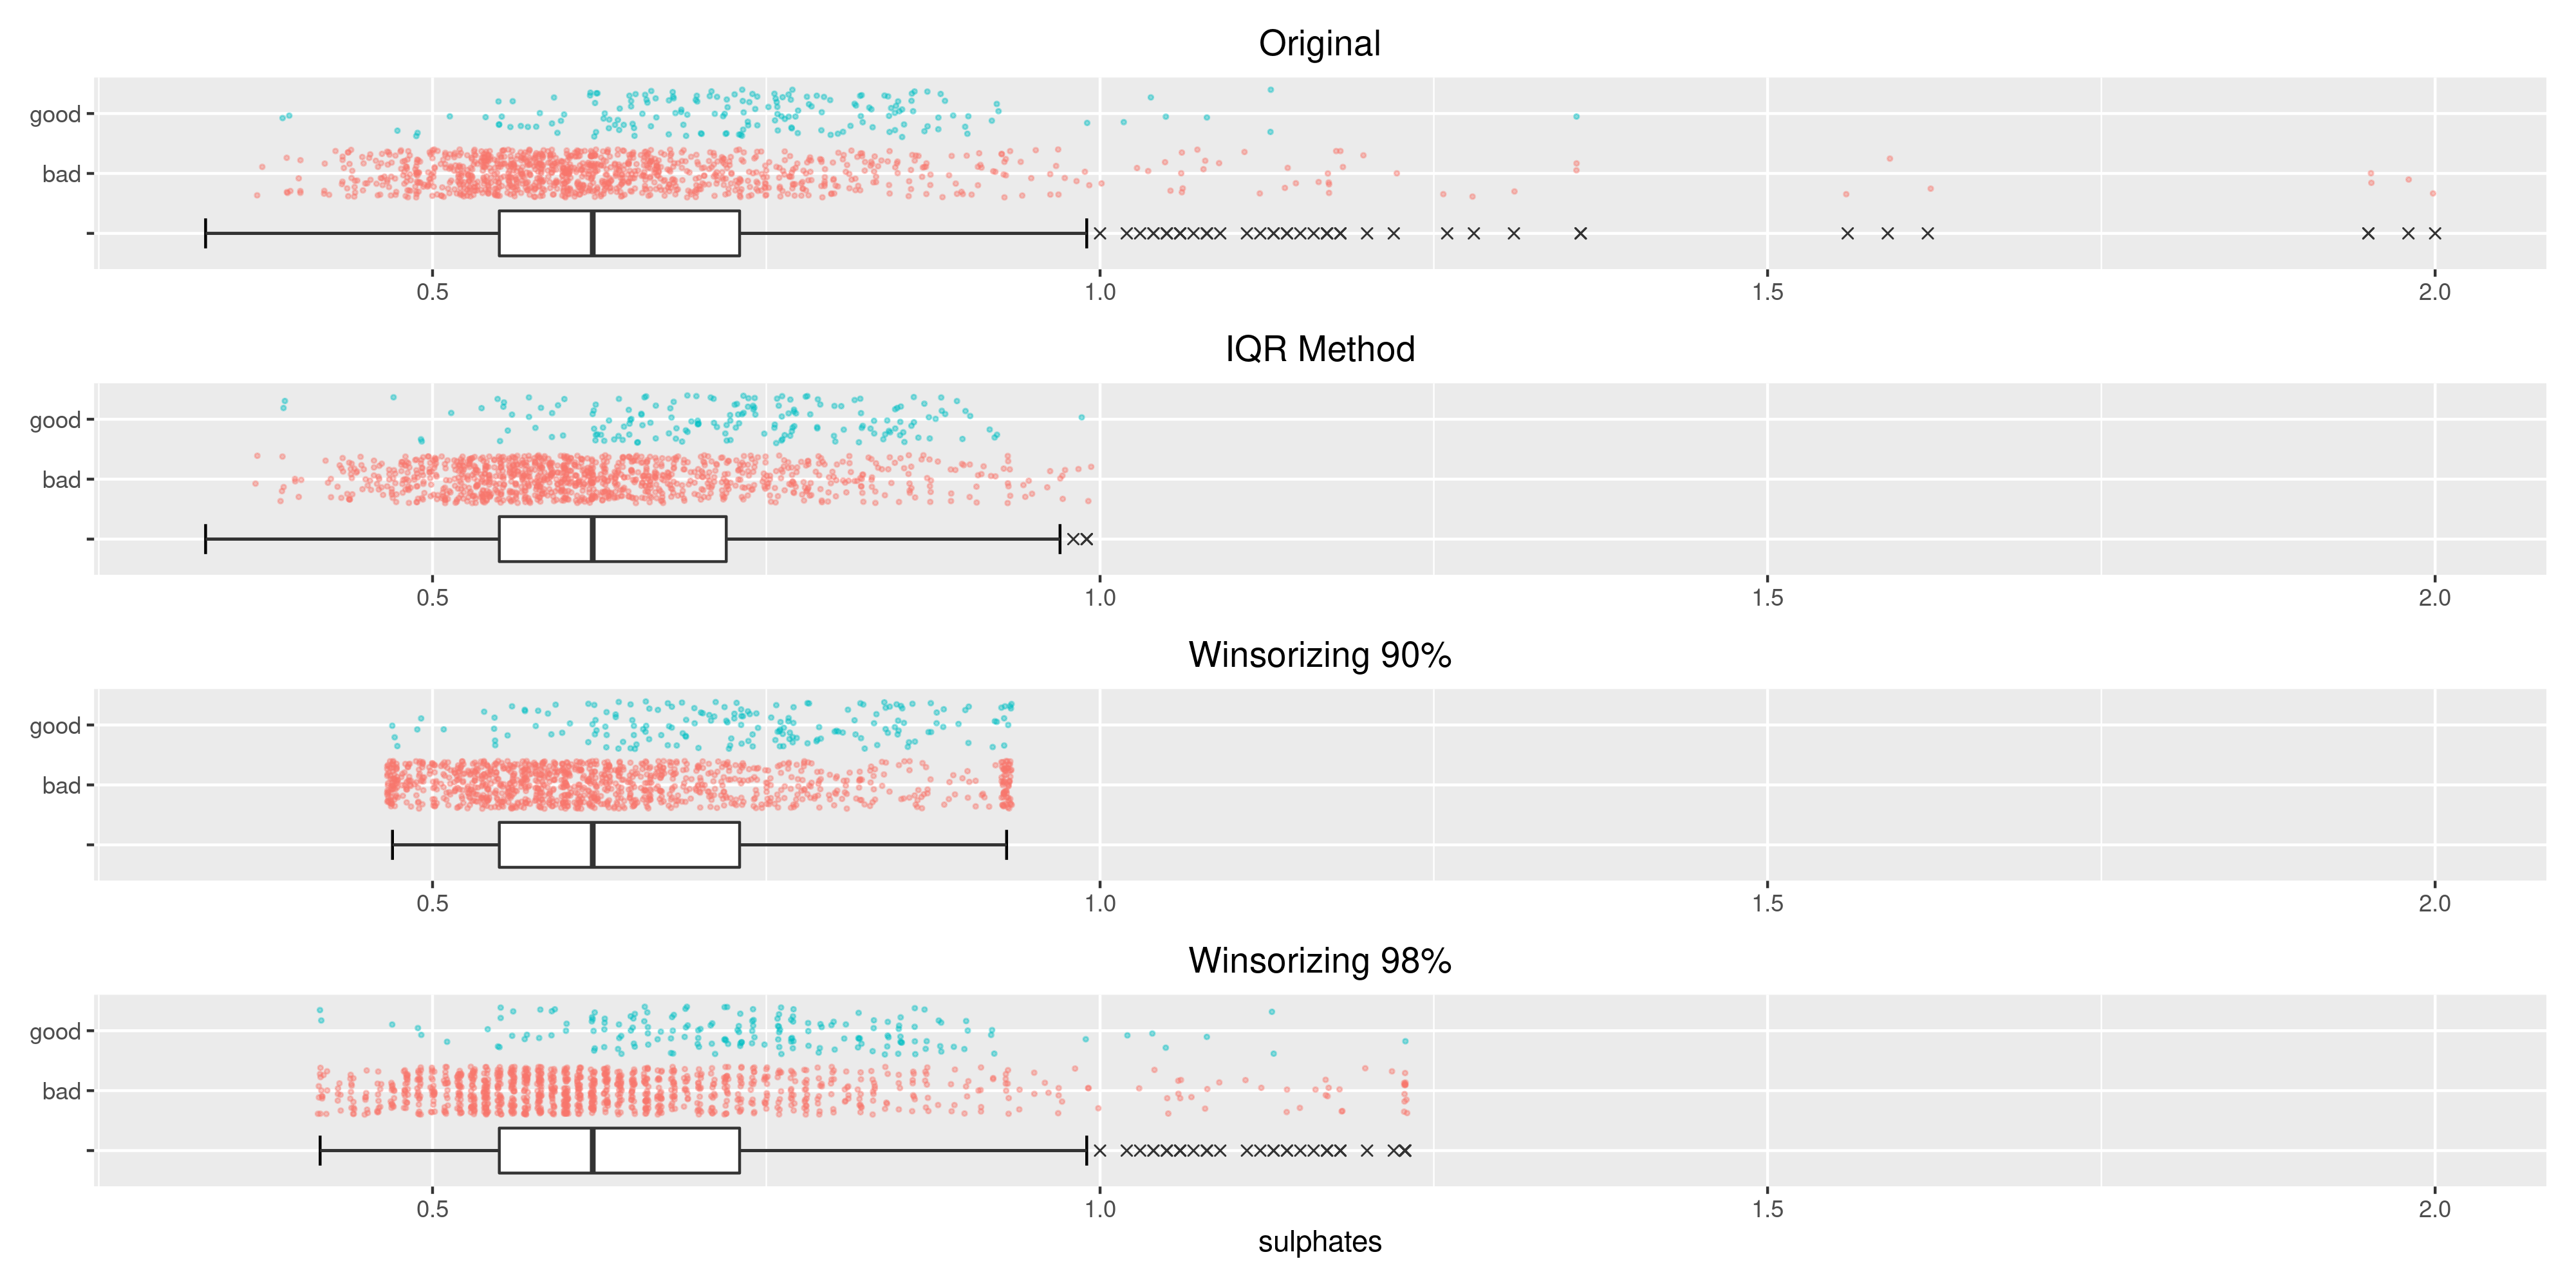
\includegraphics[width=0.99\textwidth]{images/outliers/sulphates_boxplot.png}
    }

    \subfloat[]{%
        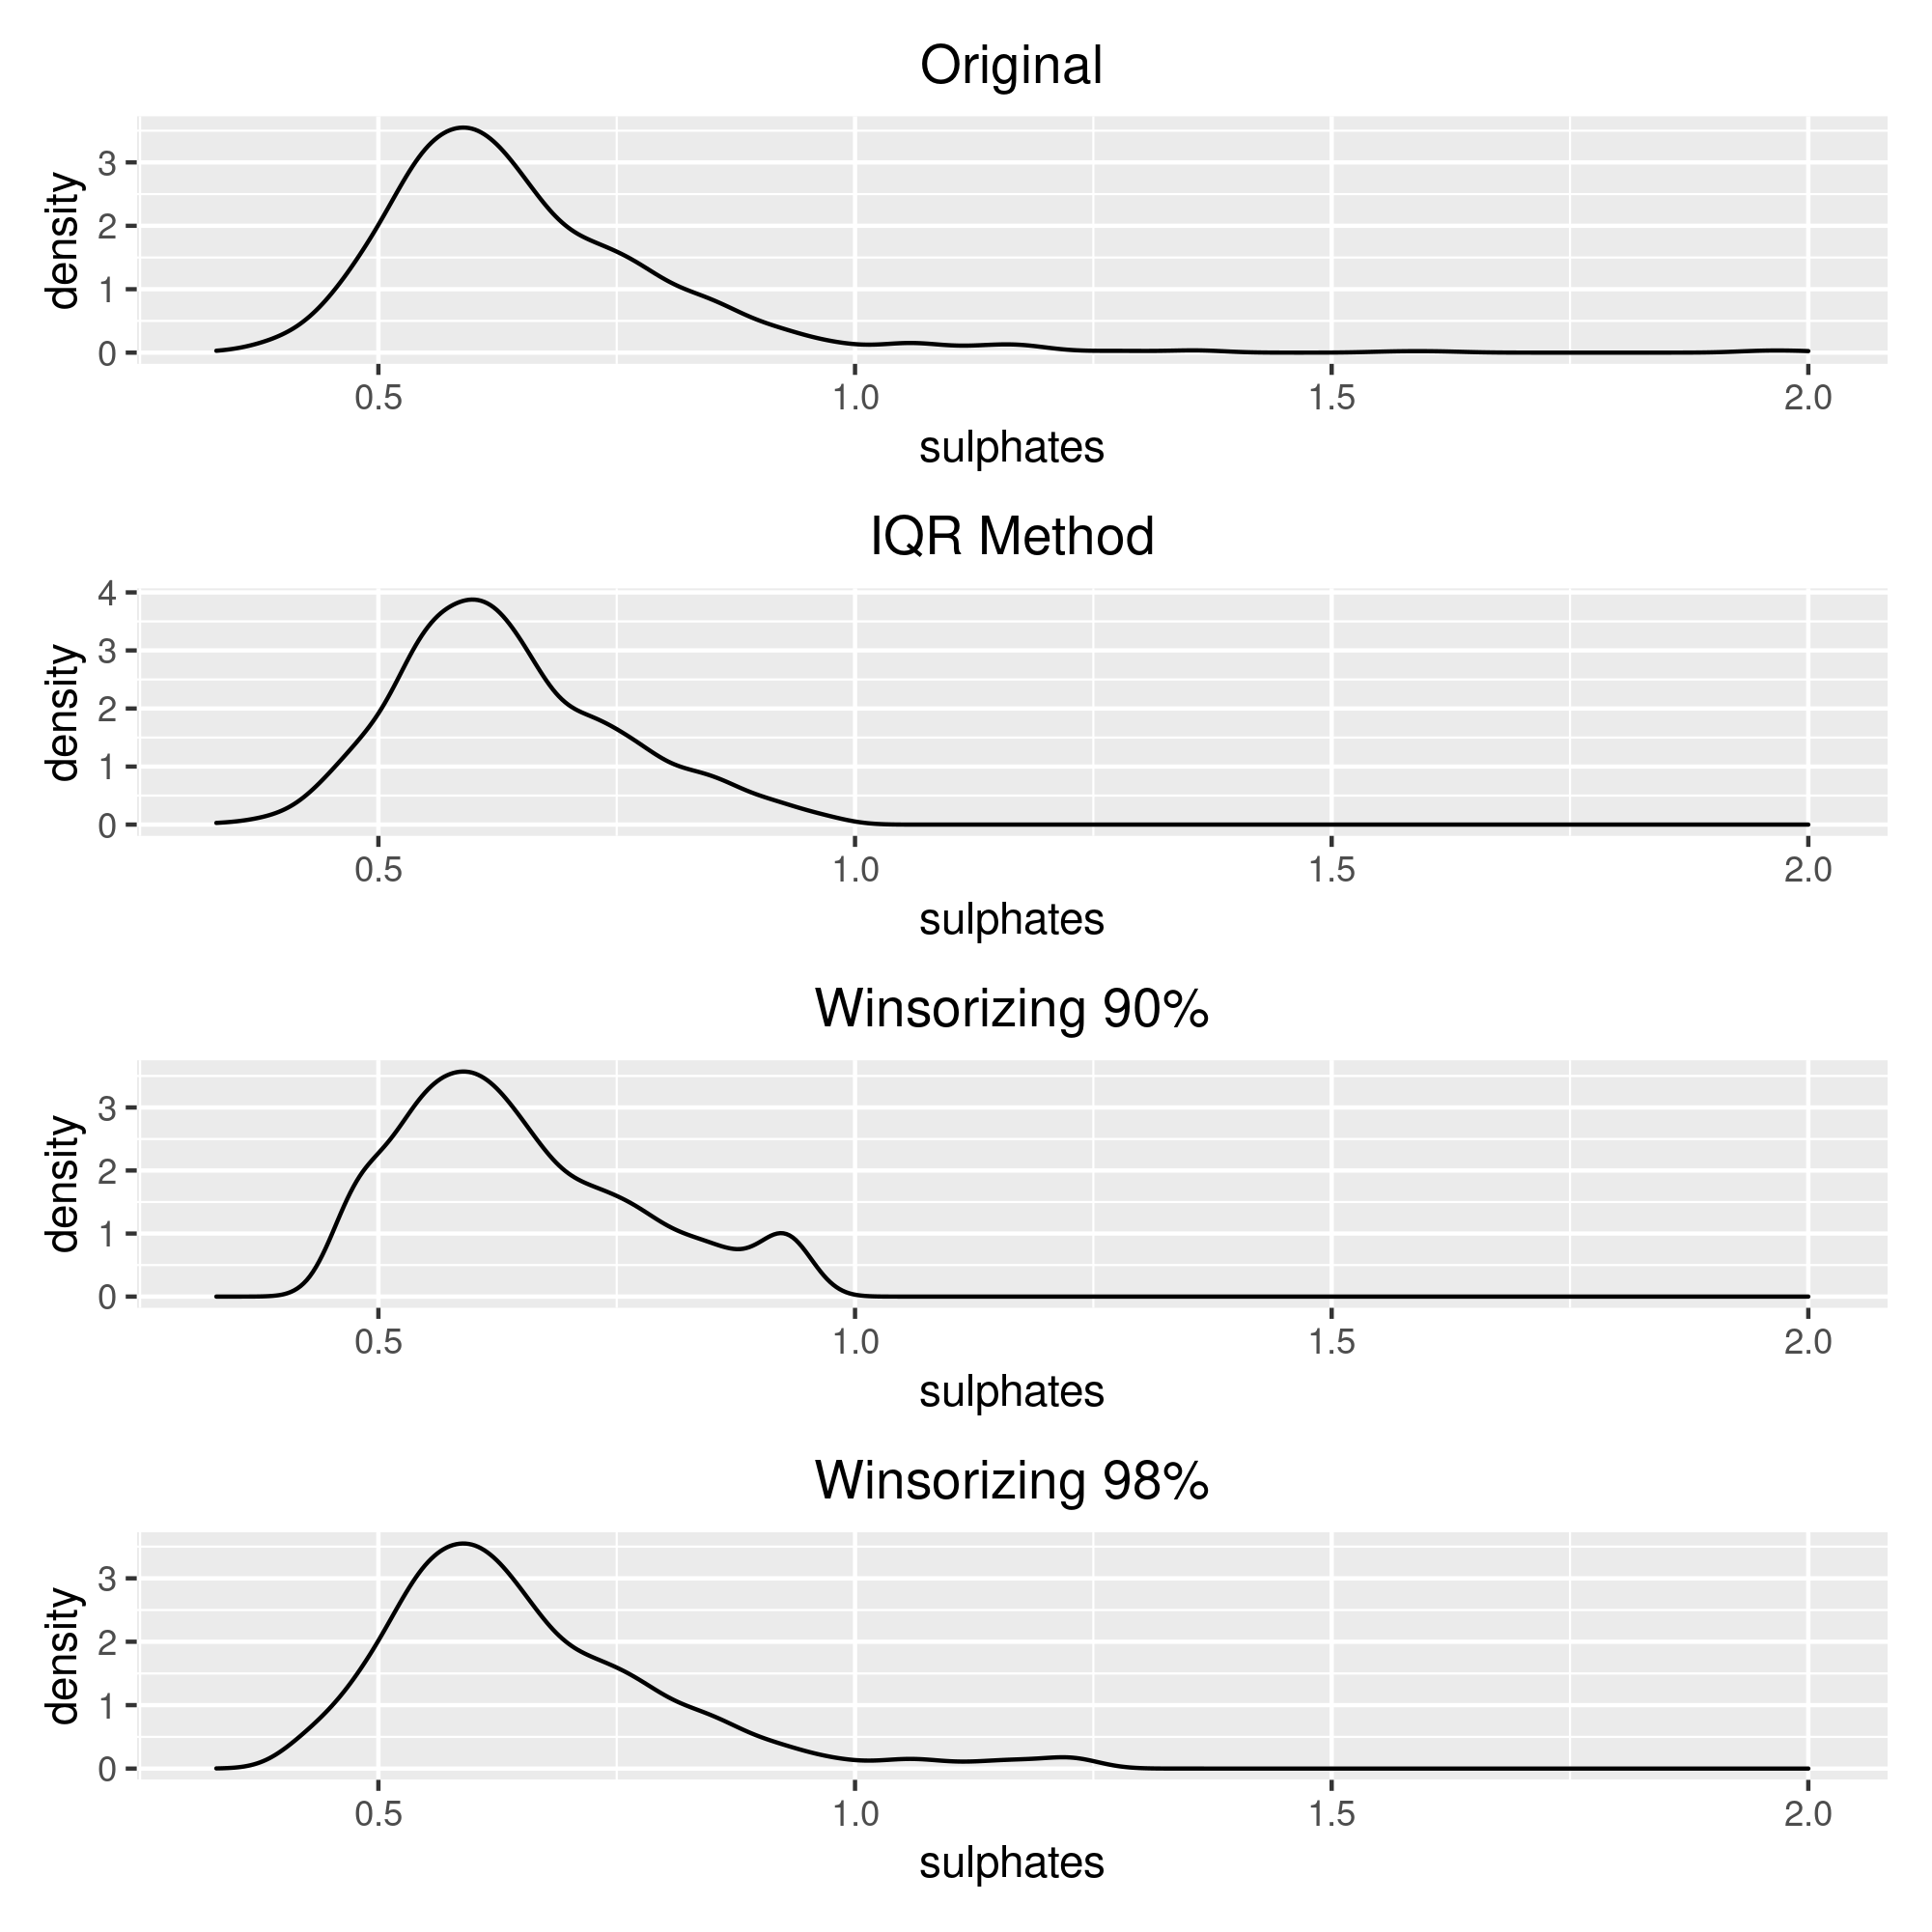
\includegraphics[width=0.45\textwidth]{images/outliers/sulphates_distribution.png}
    }\qquad
    \subfloat[]{%
        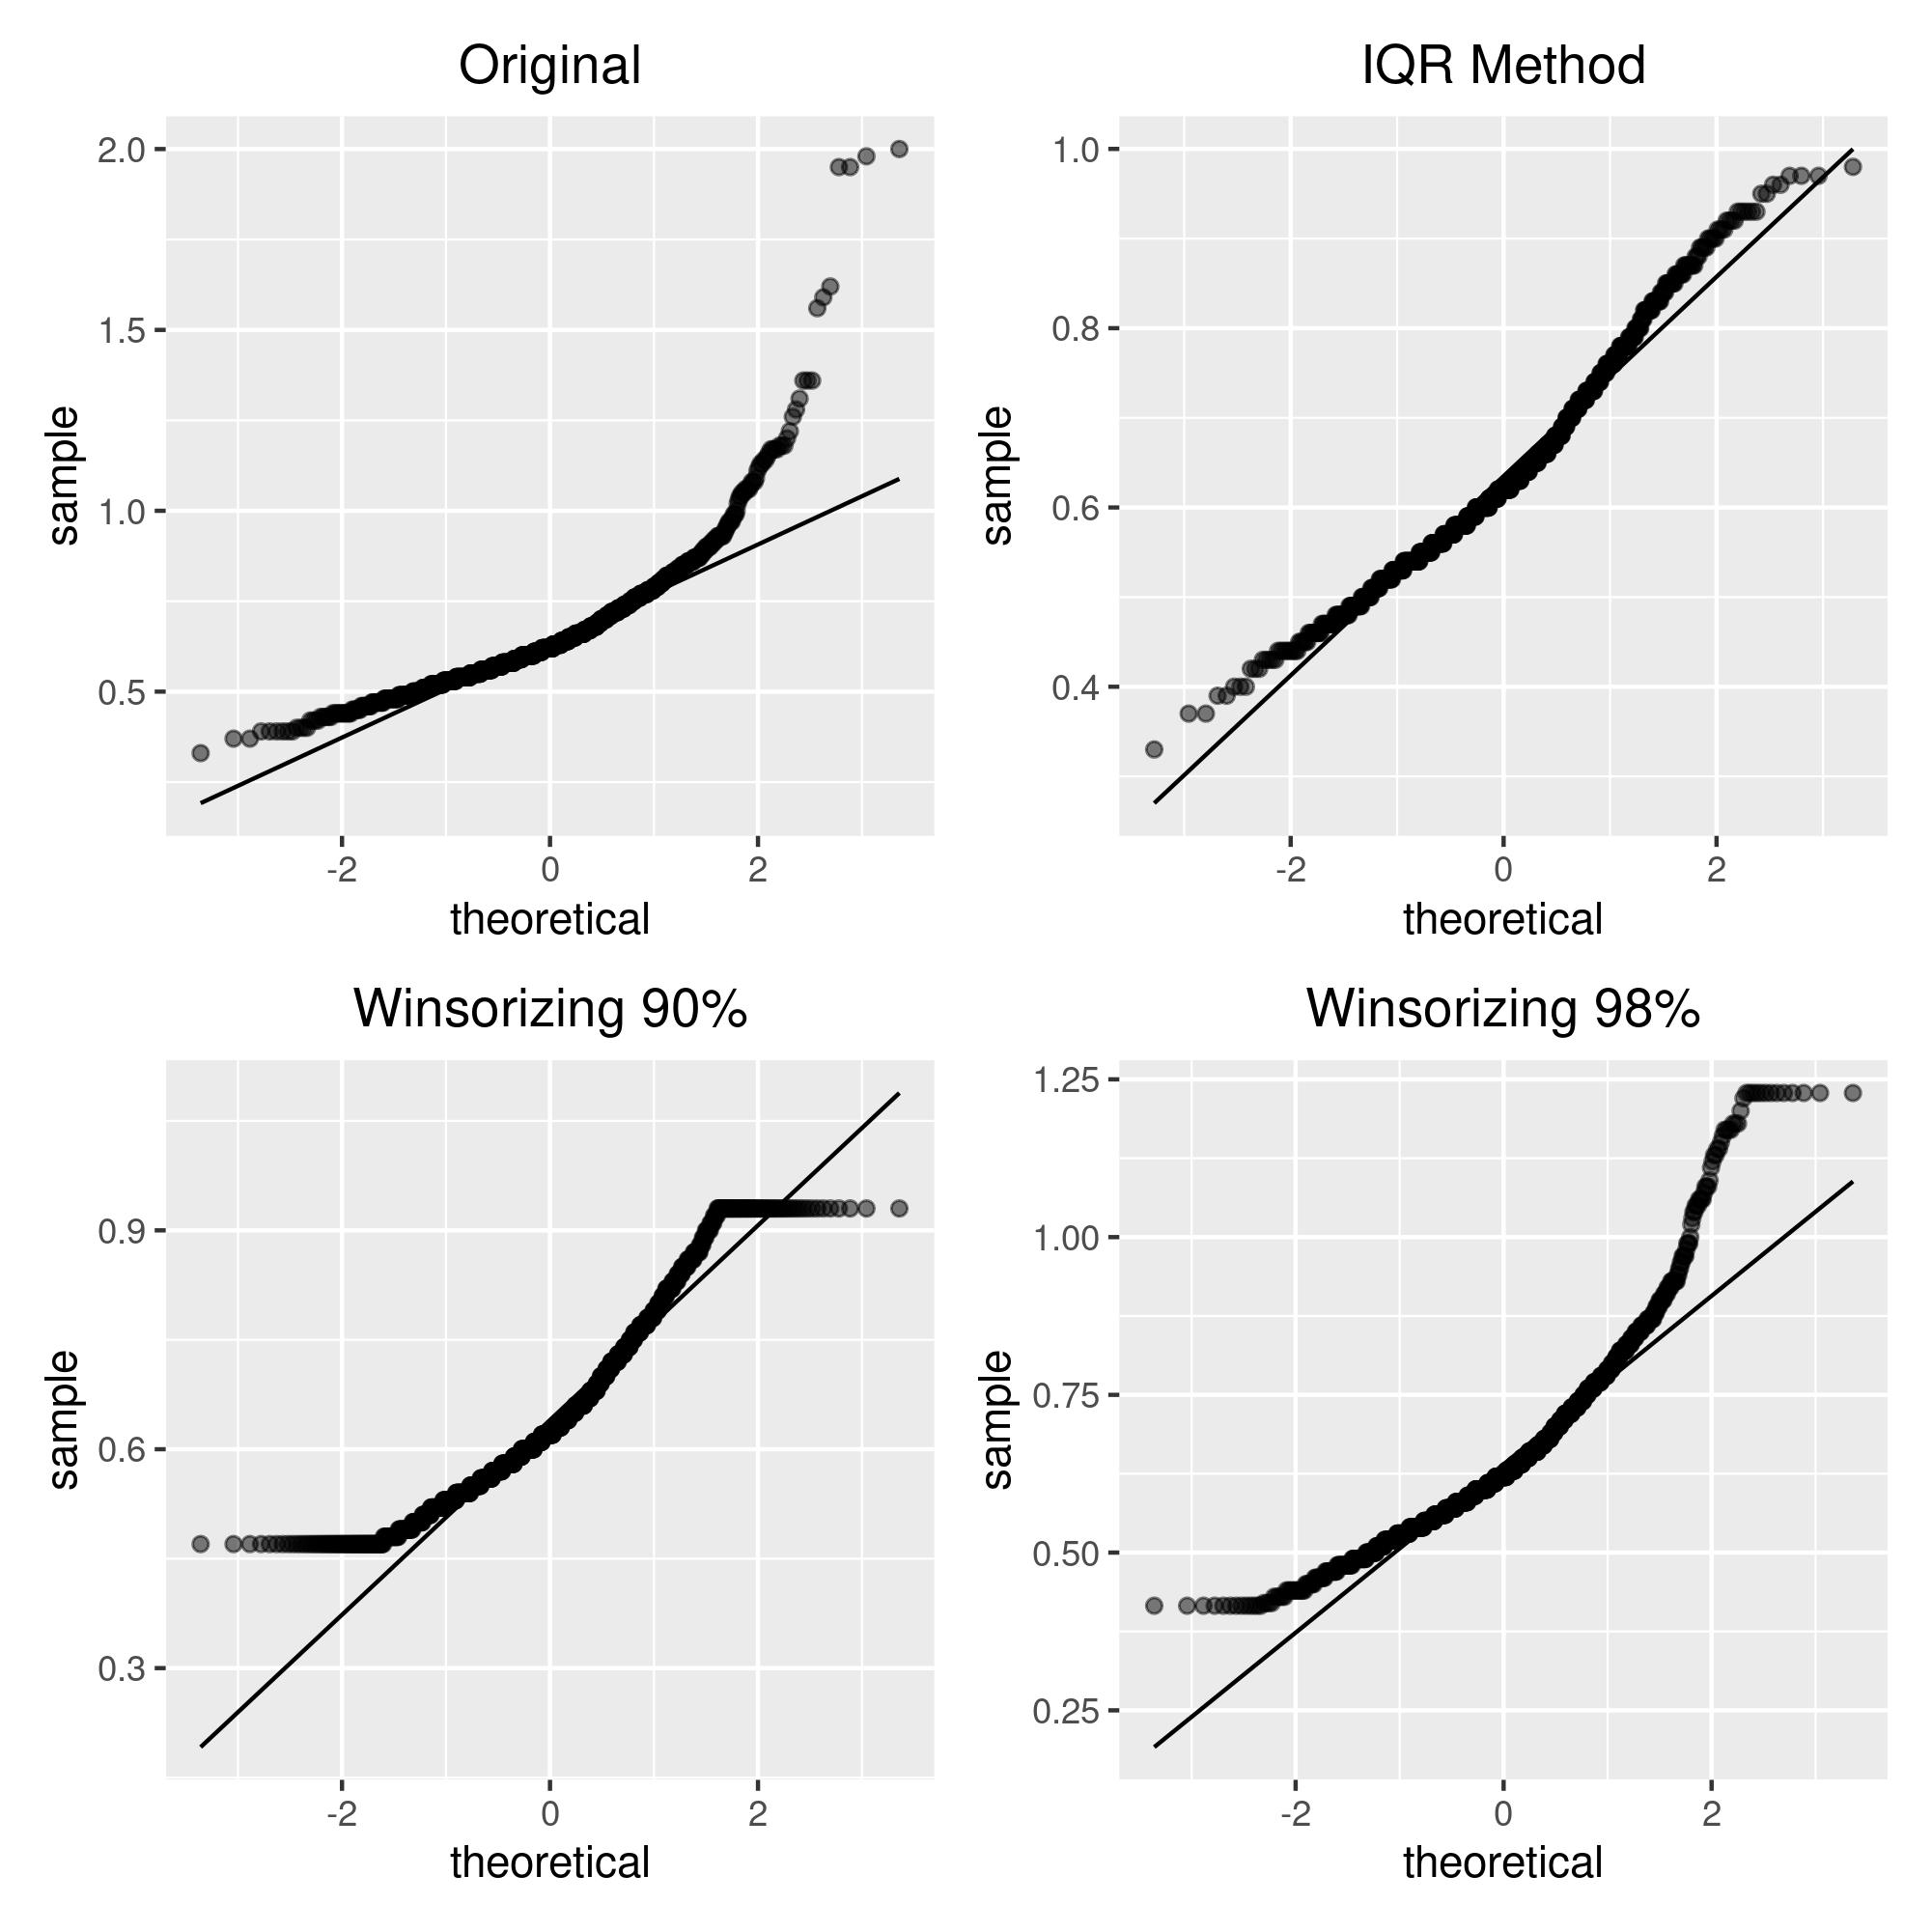
\includegraphics[width=0.45\textwidth]{images/outliers/sulphates_qqplot.png}
    }

    \label{fig:sulphates}
    \caption{Commento}
\end{figure}

\begin{figure}[H]
    \centering

    \subfloat[]{%
        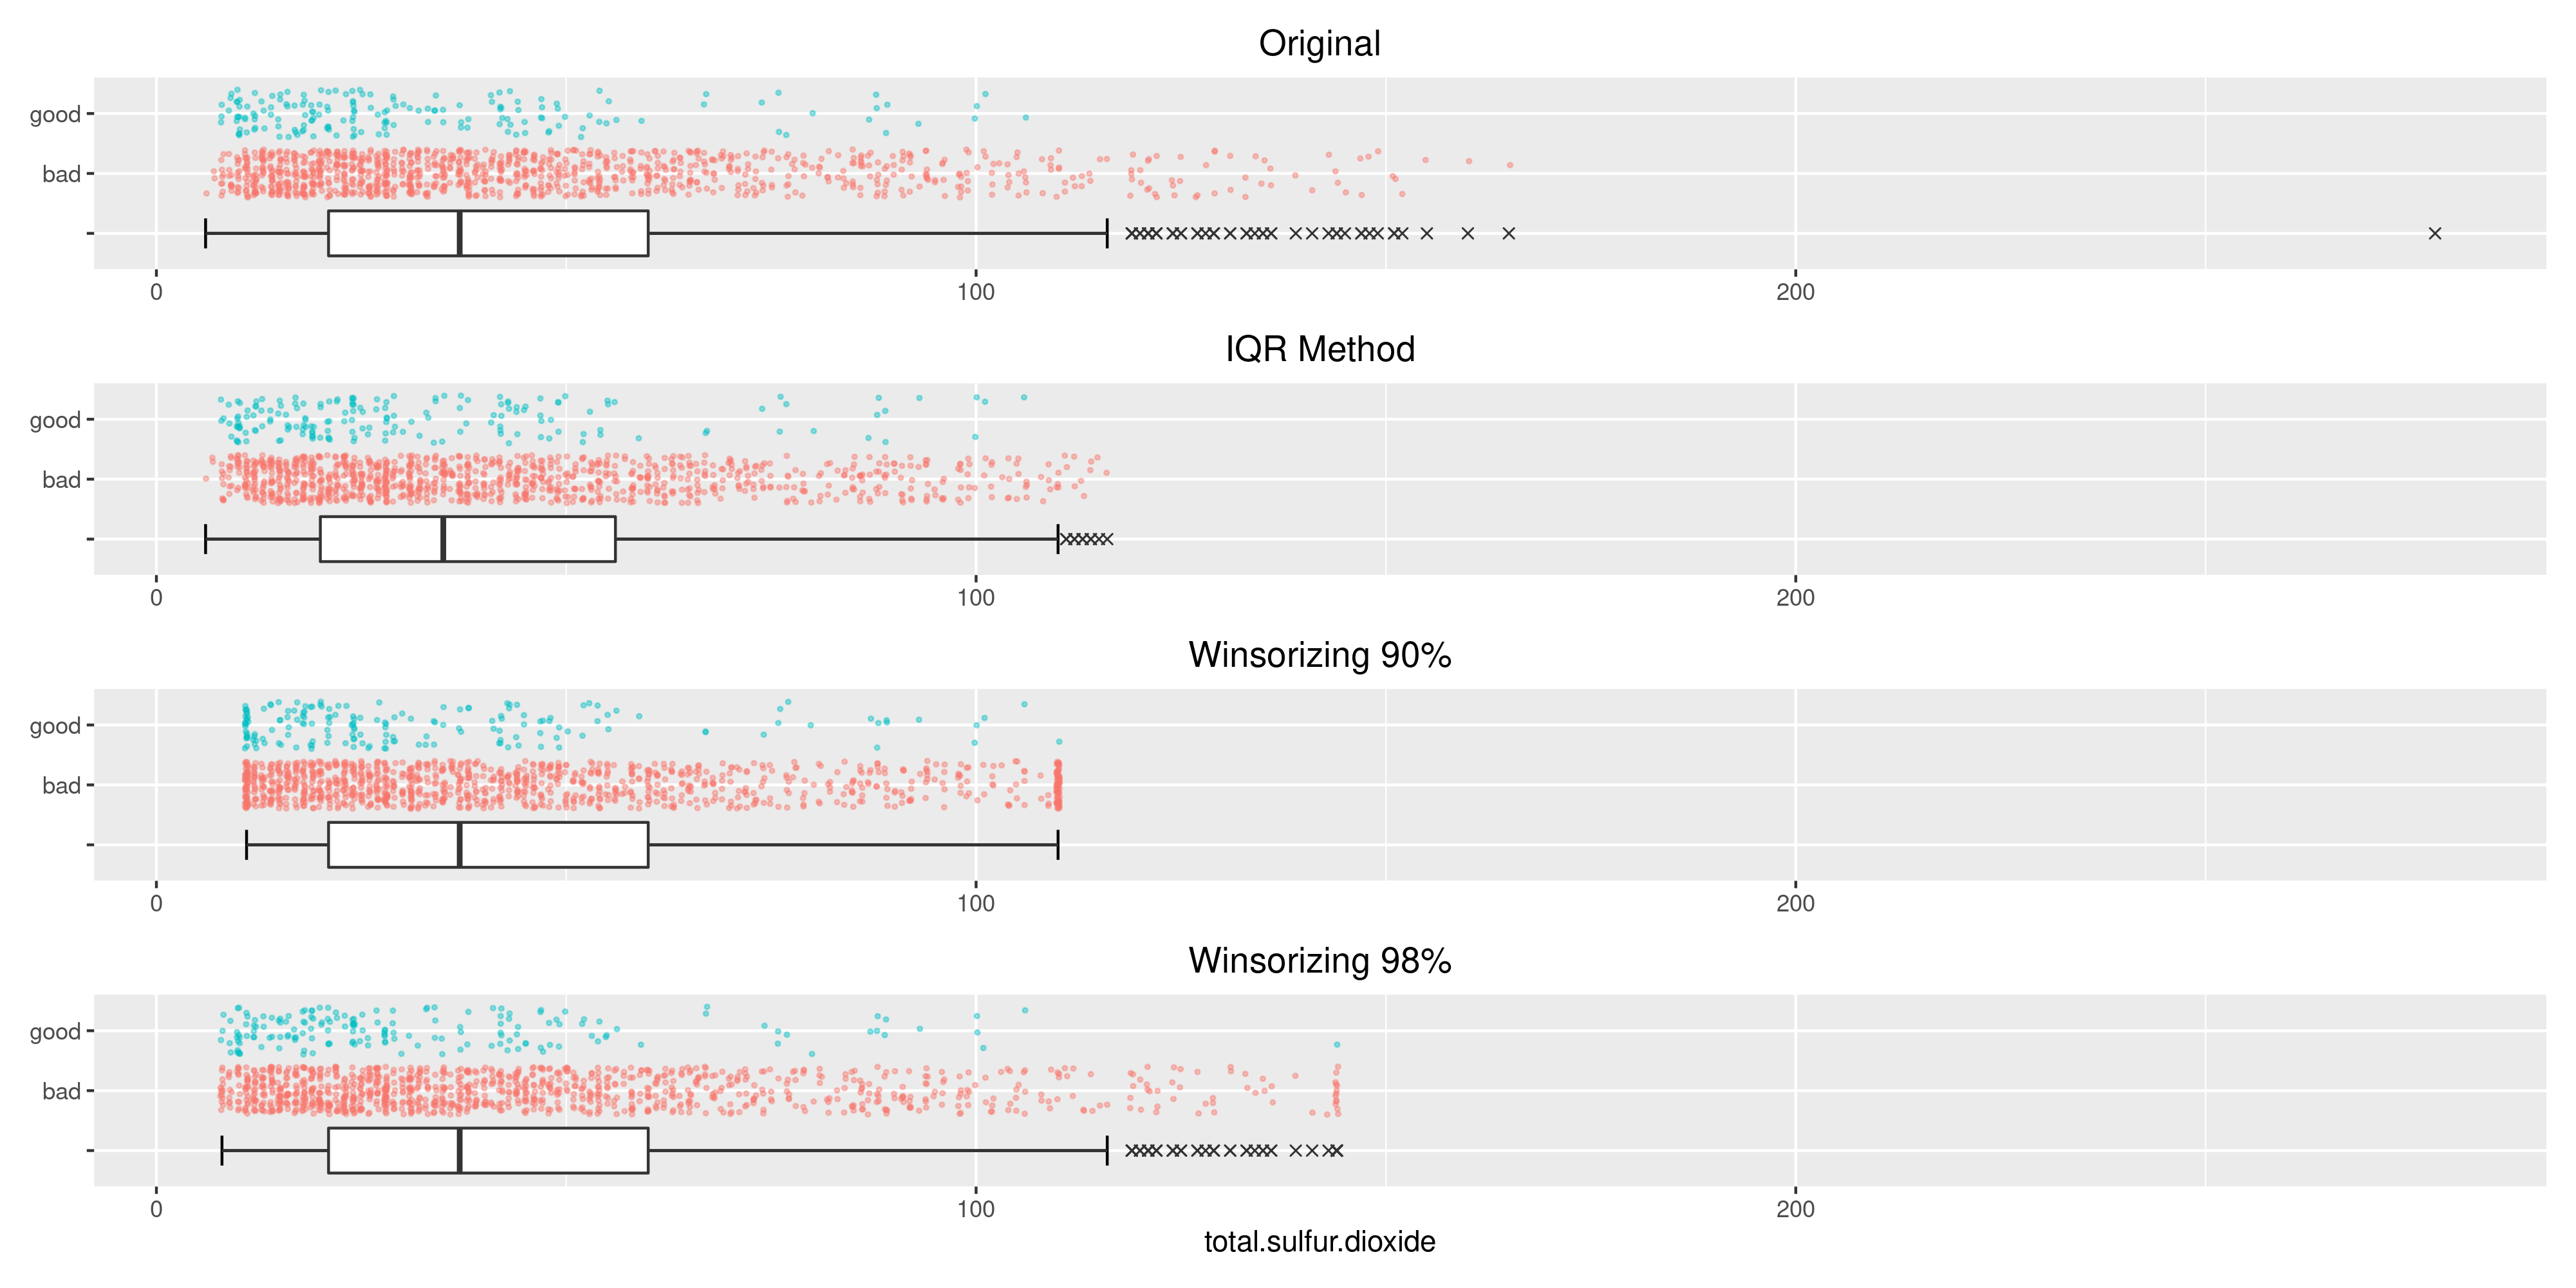
\includegraphics[width=0.99\textwidth]{images/outliers/total.sulfur.dioxide_boxplot.png}
    }

    \subfloat[]{%
        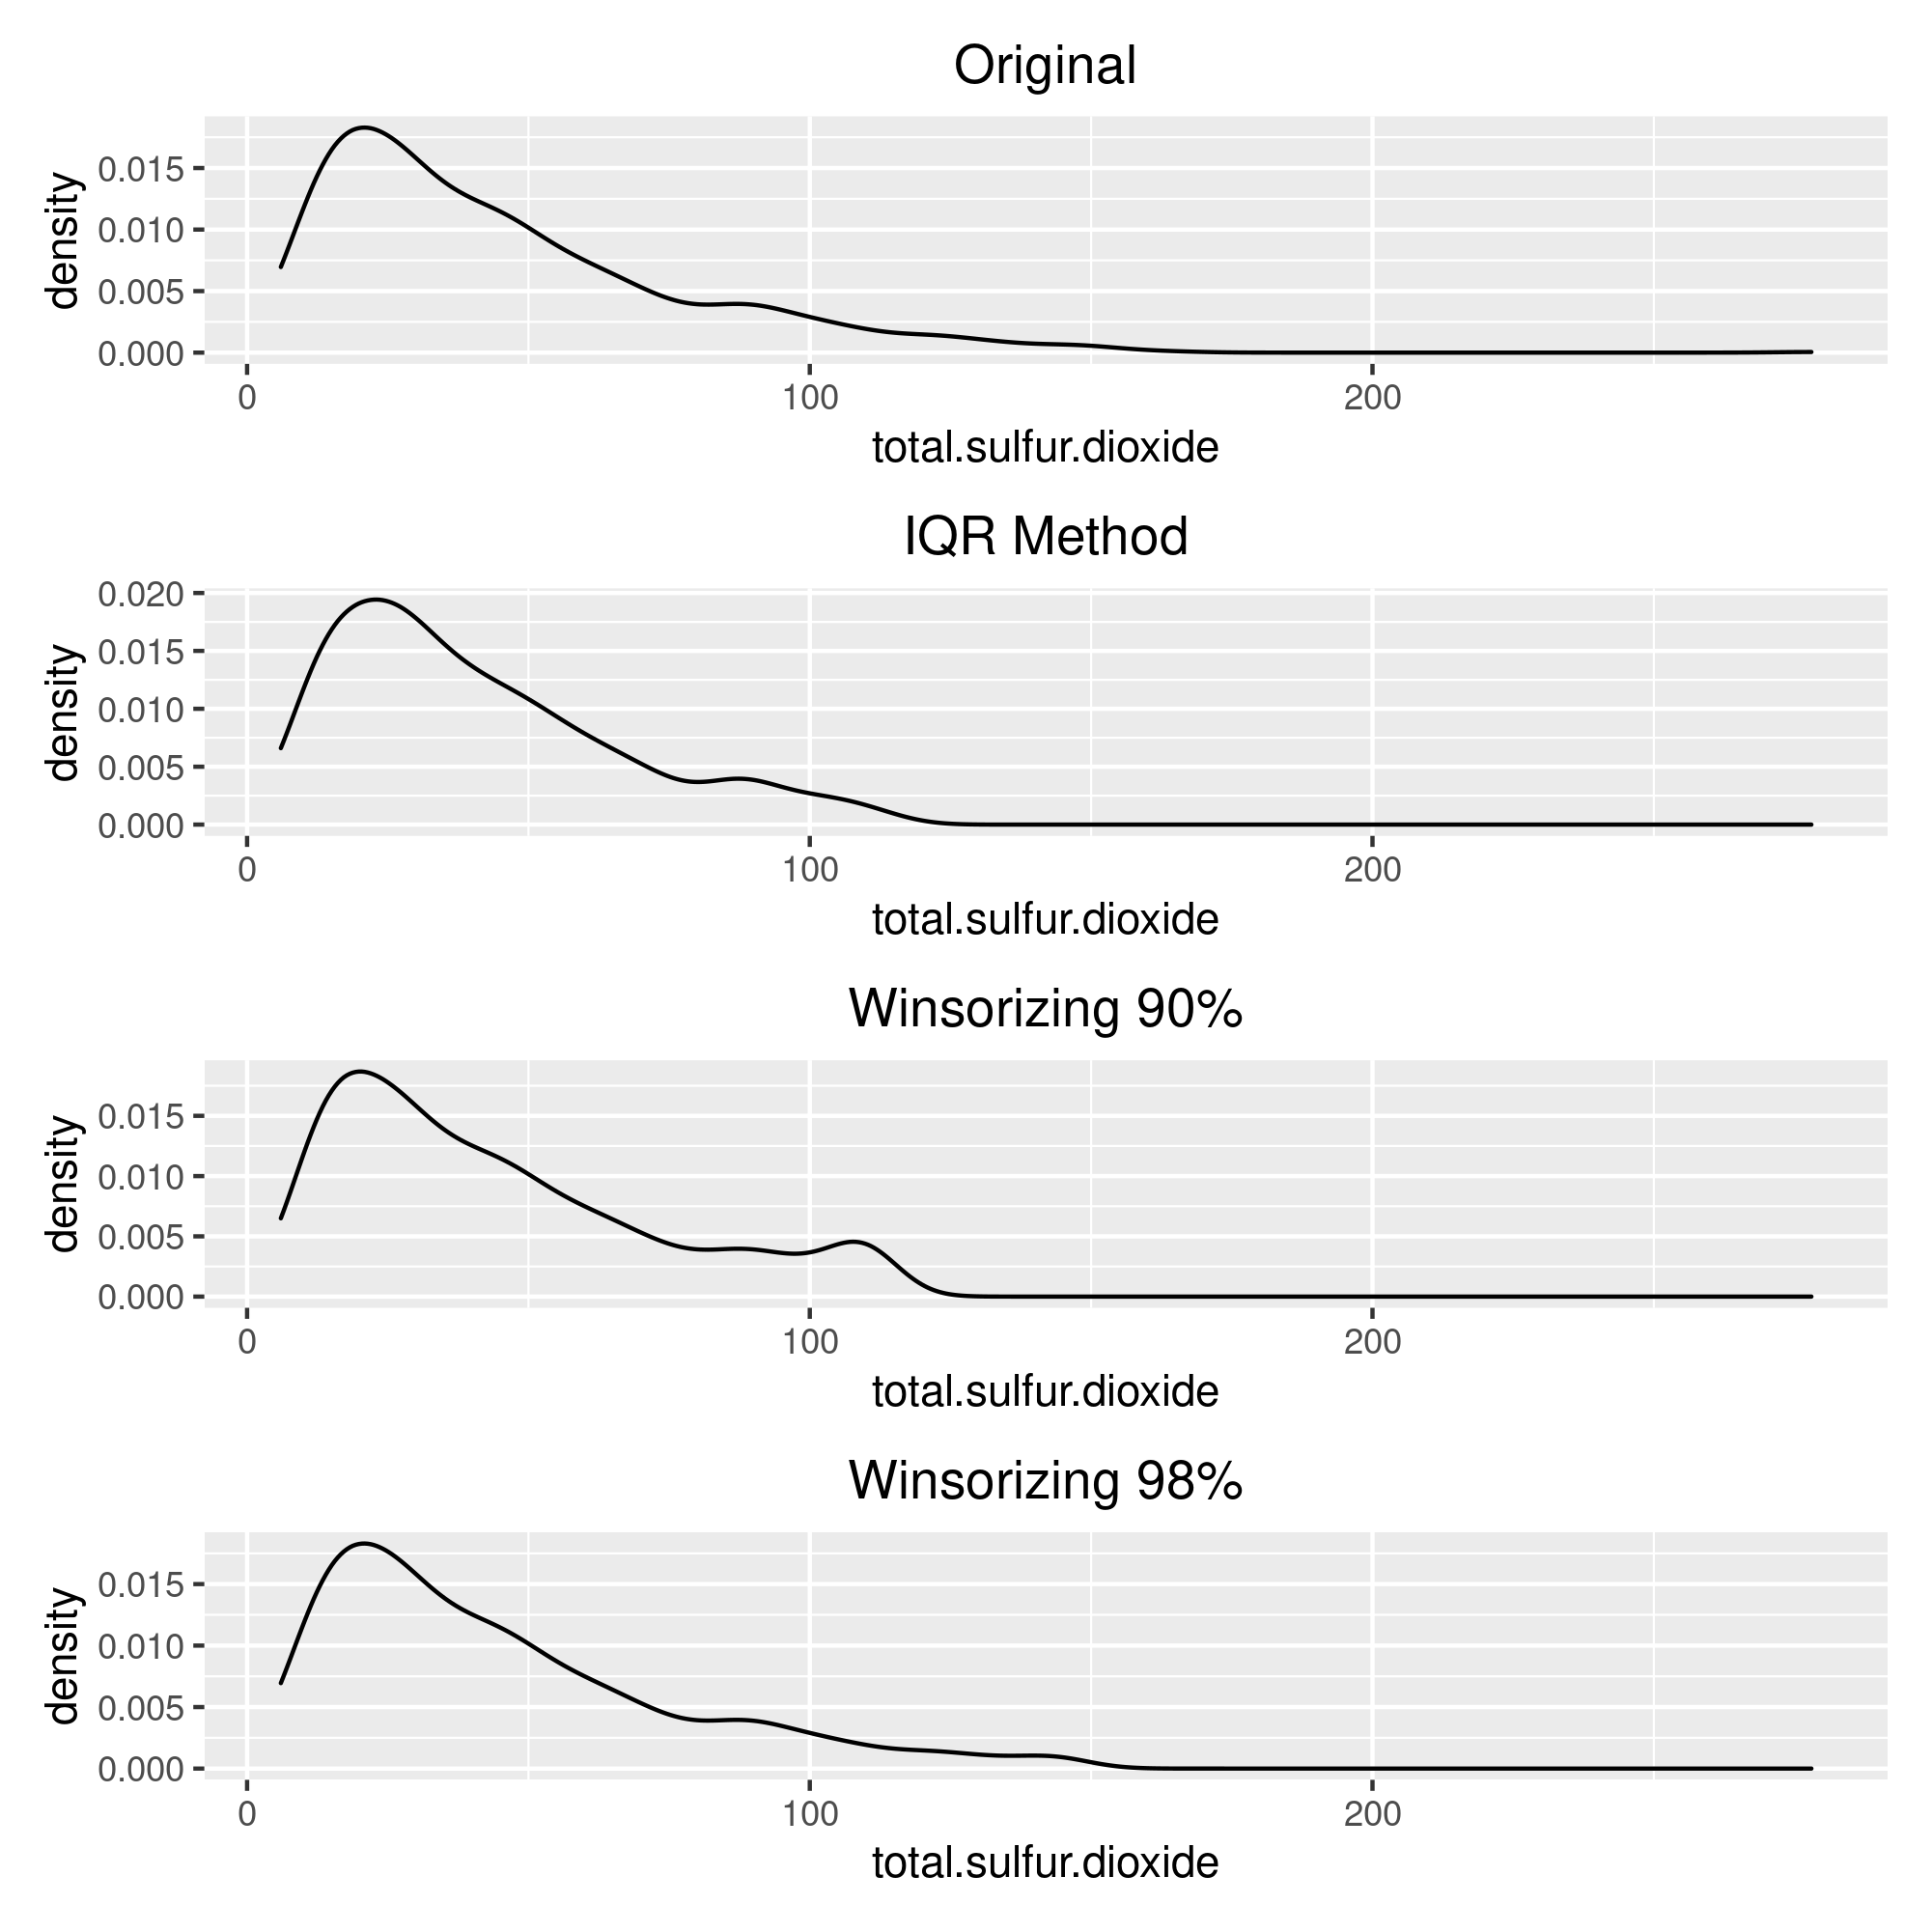
\includegraphics[width=0.45\textwidth]{images/outliers/total.sulfur.dioxide_distribution.png}
    }\qquad
    \subfloat[]{%
        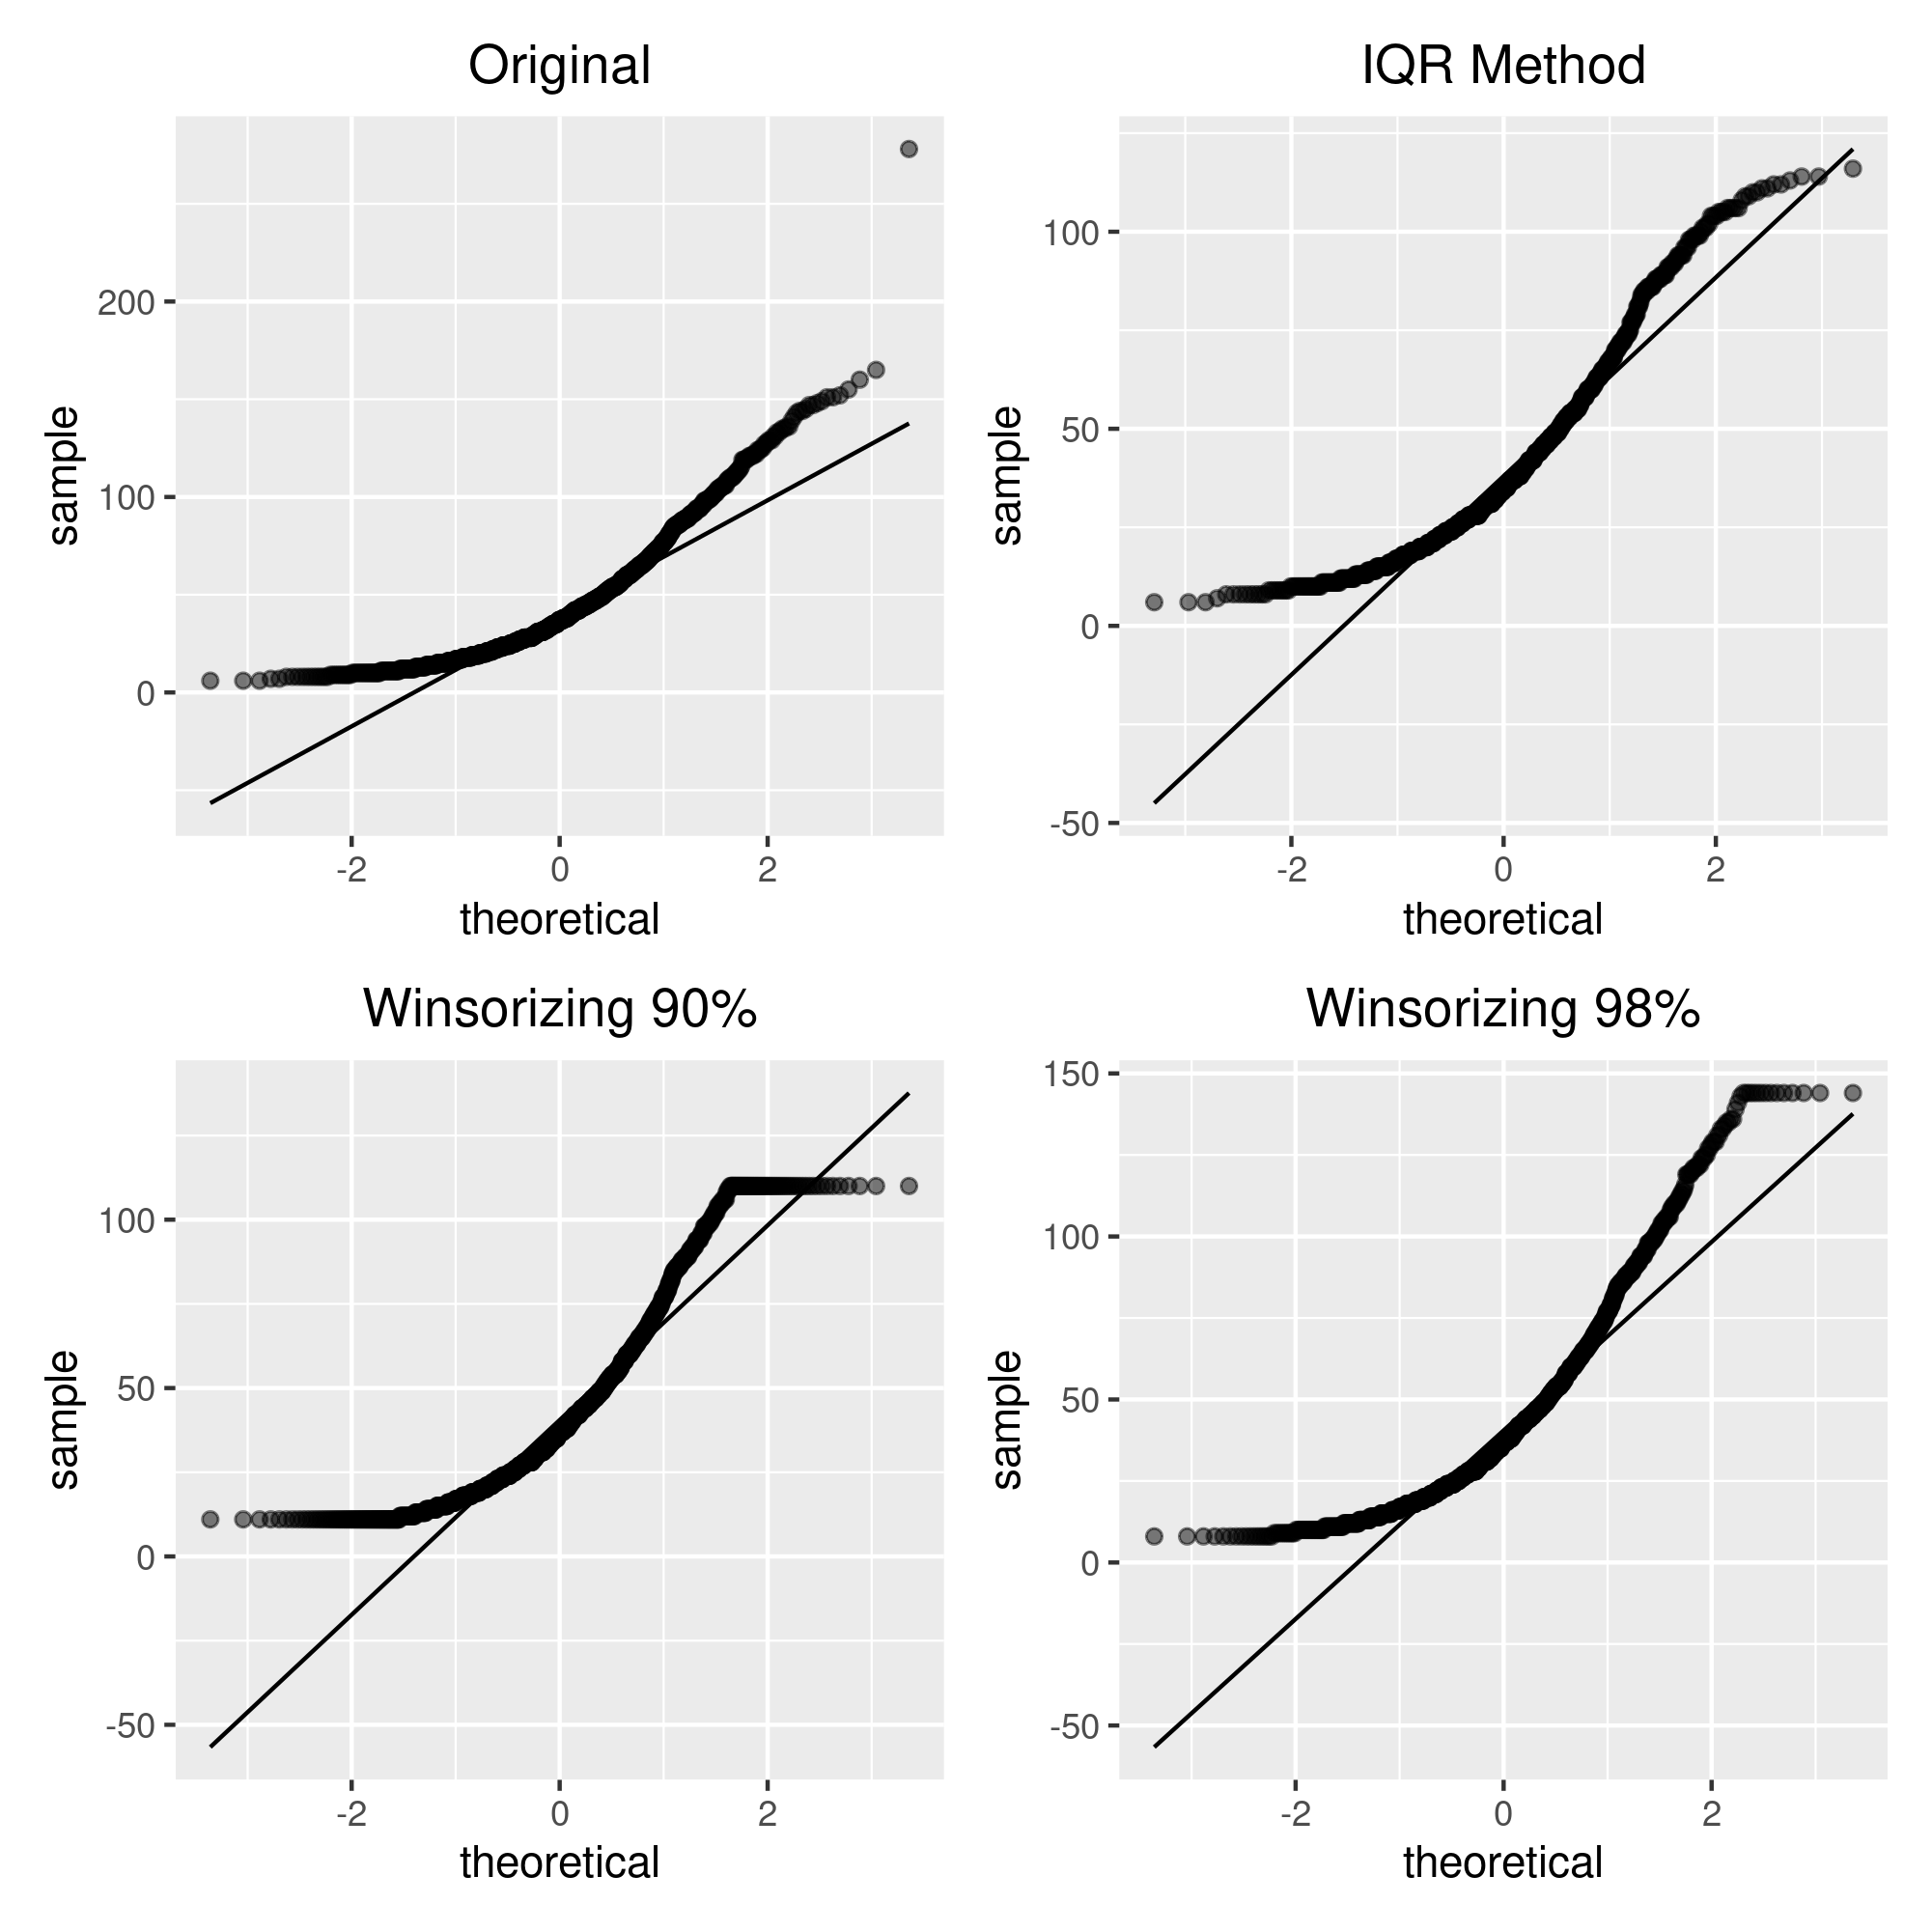
\includegraphics[width=0.45\textwidth]{images/outliers/total.sulfur.dioxide_qqplot.png}
    }

    \label{fig:total.sulfur.dioxide}
    \caption{Commento}
\end{figure}

\begin{figure}[H]
    \centering

    \subfloat[]{%
        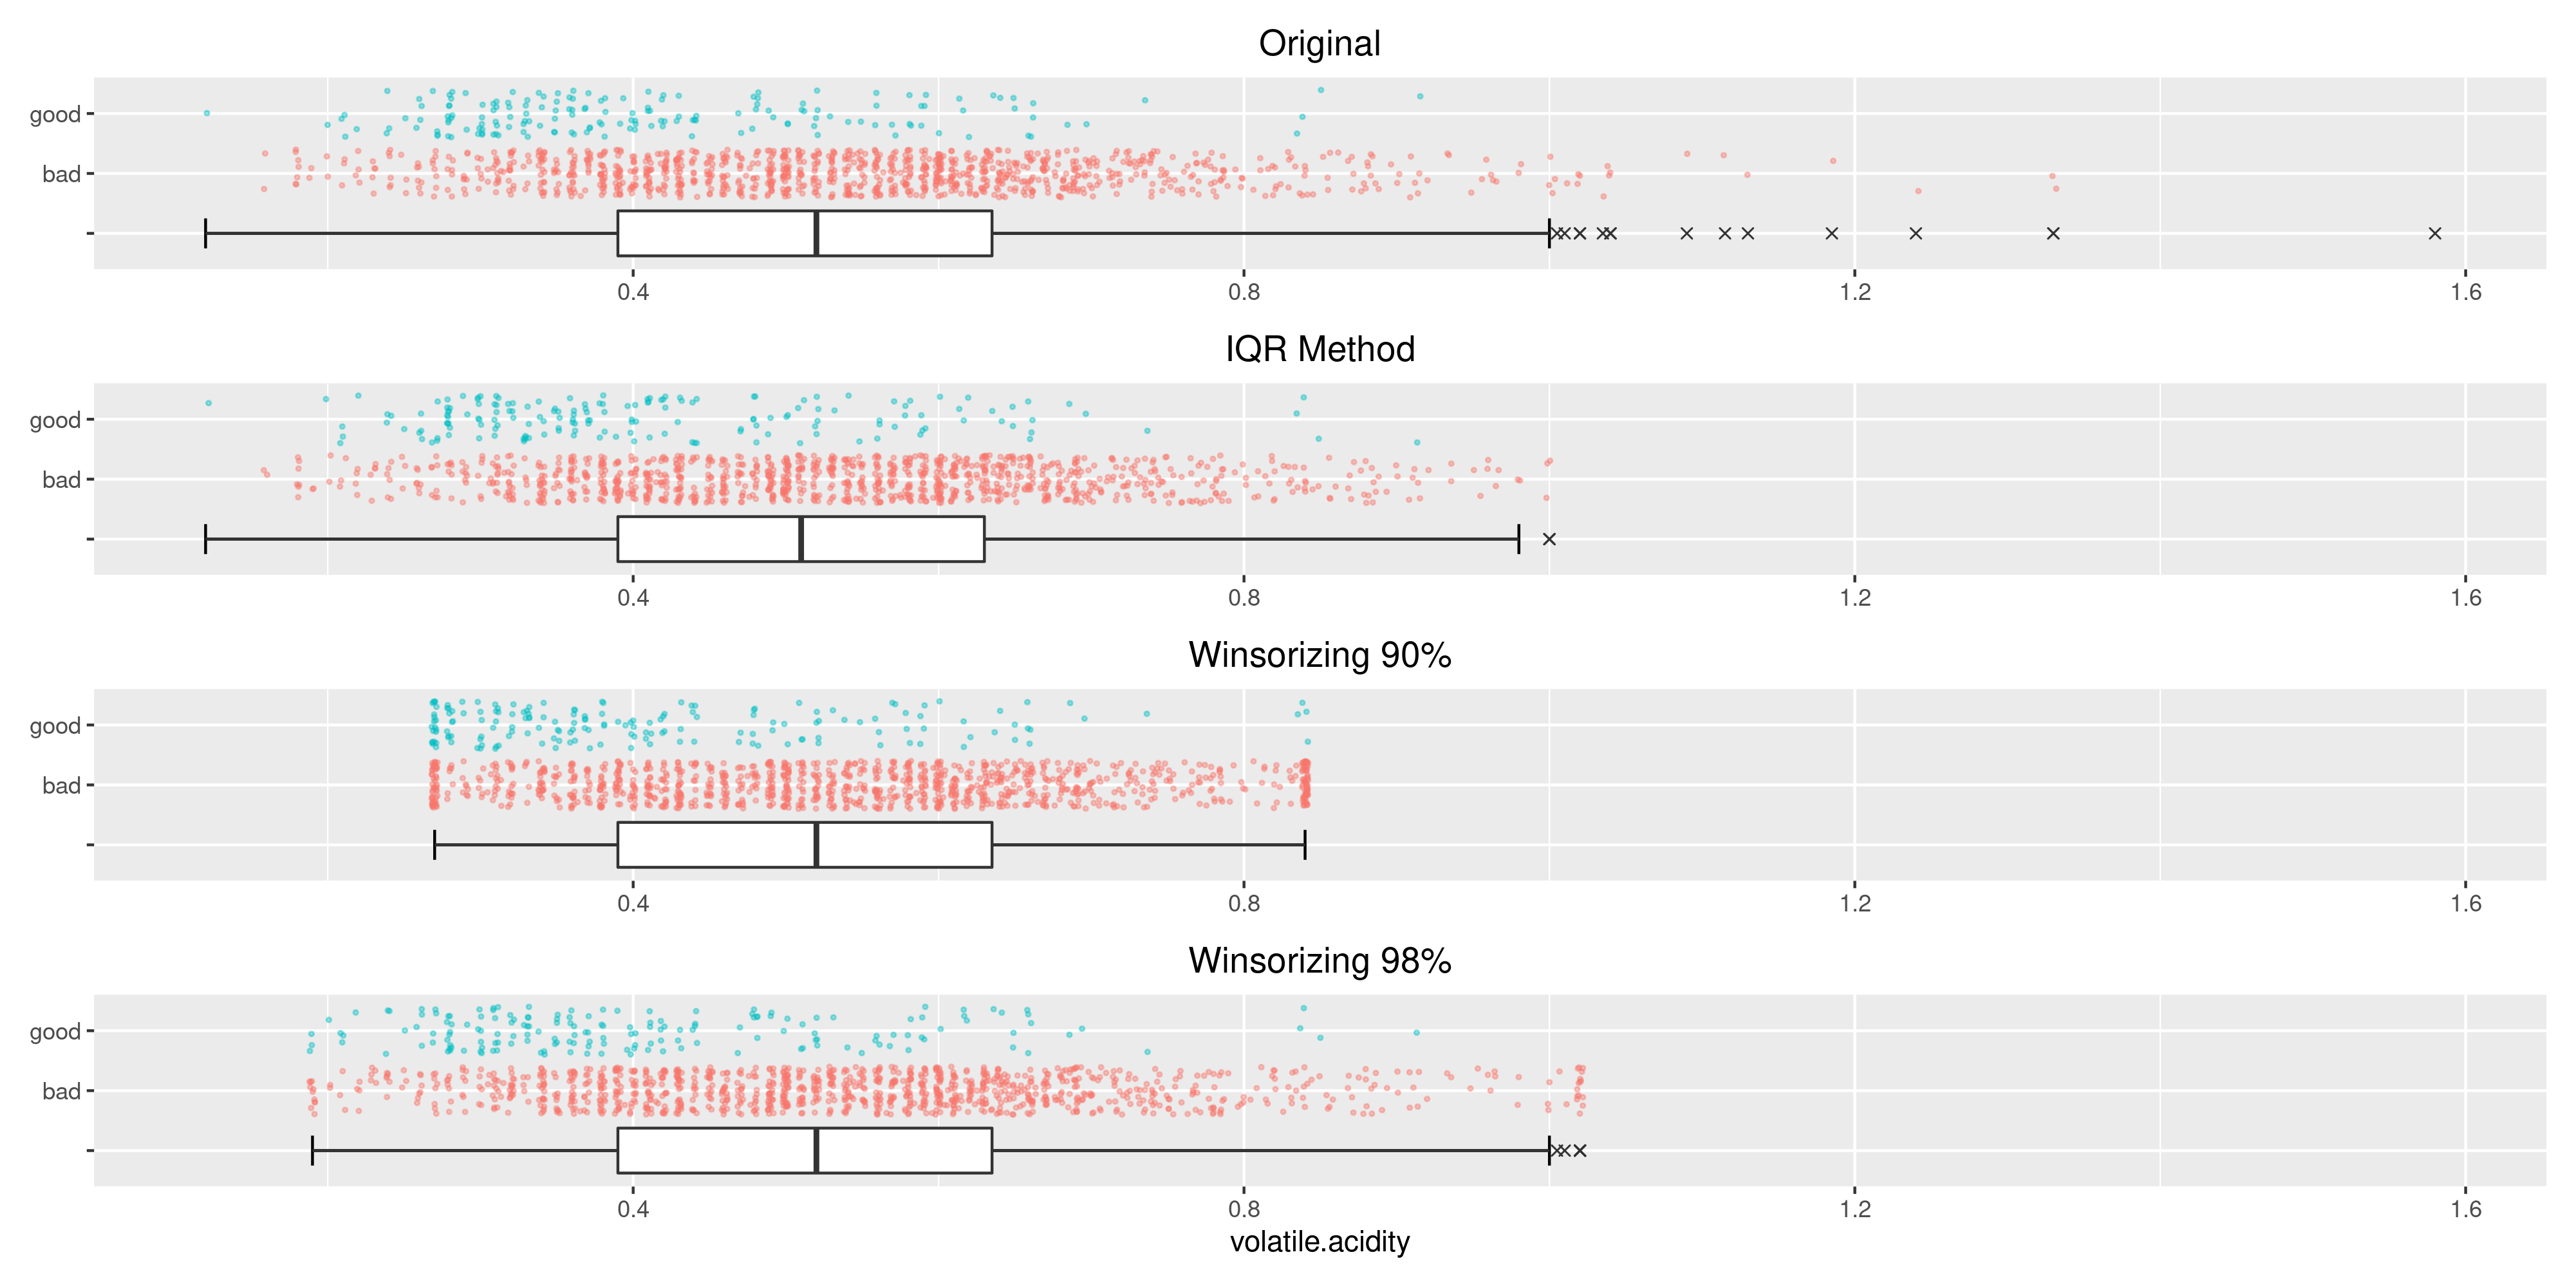
\includegraphics[width=0.99\textwidth]{images/outliers/volatile.acidity_boxplot.png}
    }

    \subfloat[]{%
        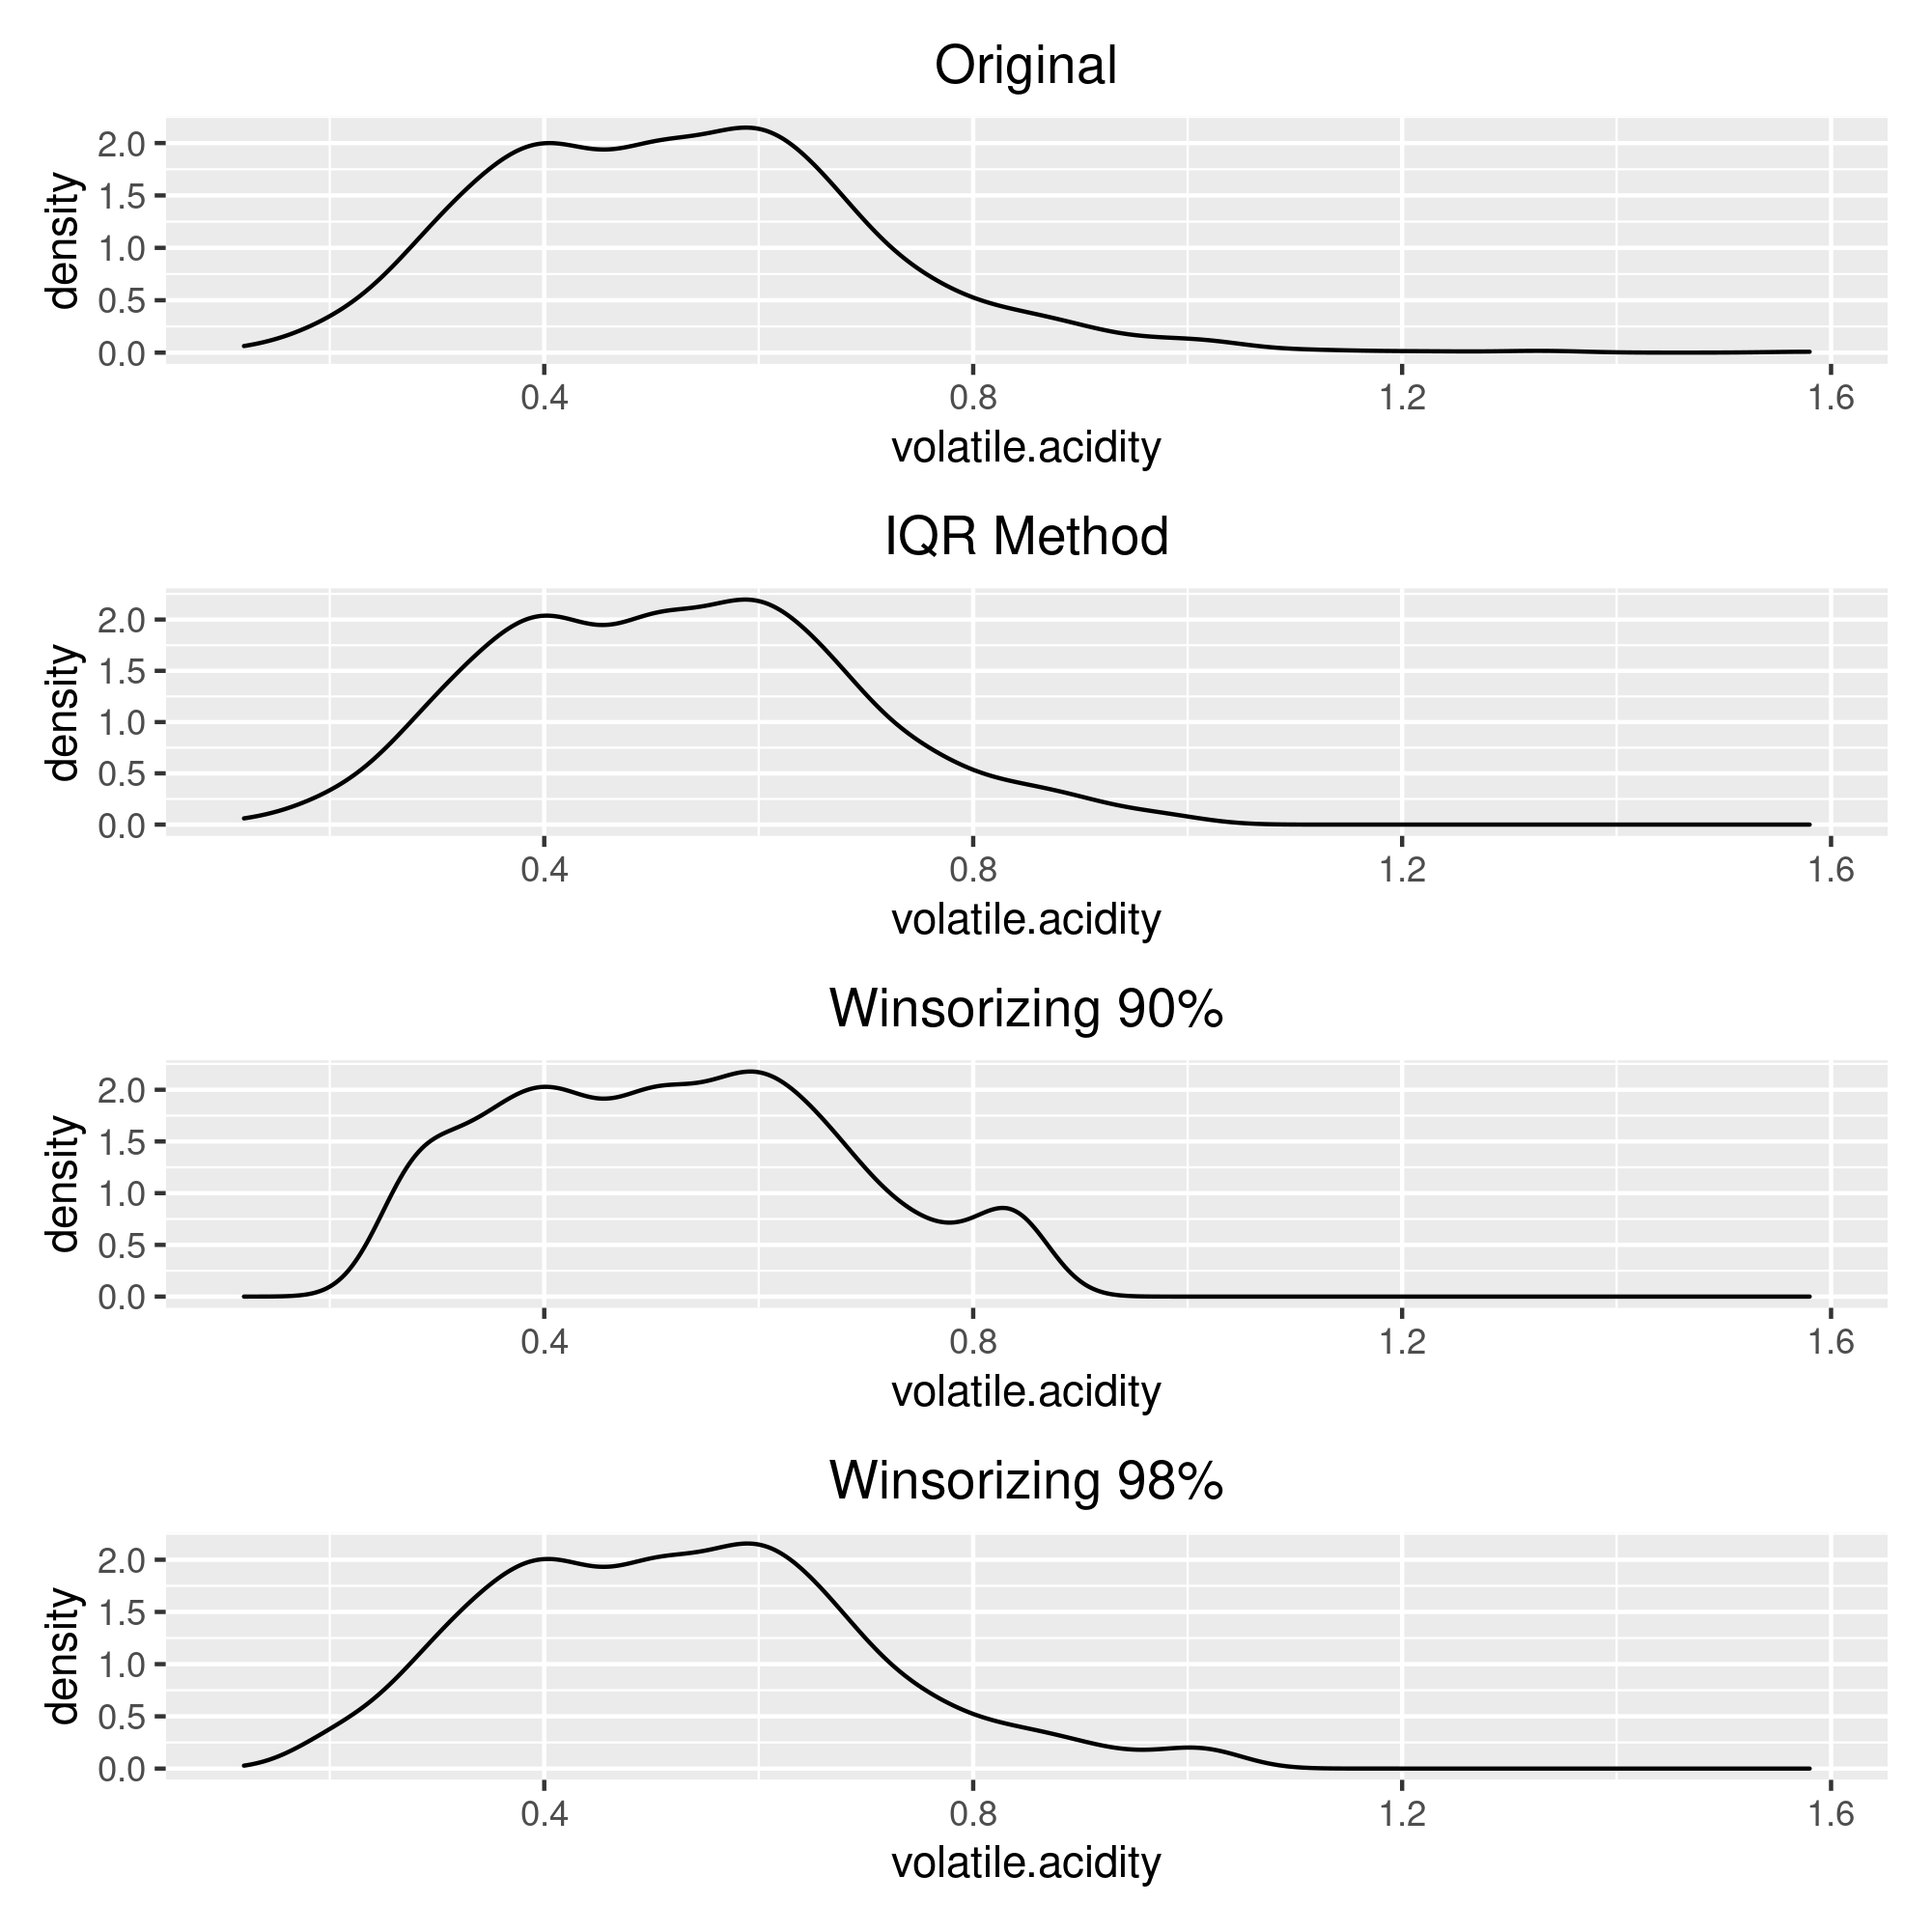
\includegraphics[width=0.45\textwidth]{images/outliers/volatile.acidity_distribution.png}
    }\qquad
    \subfloat[]{%
        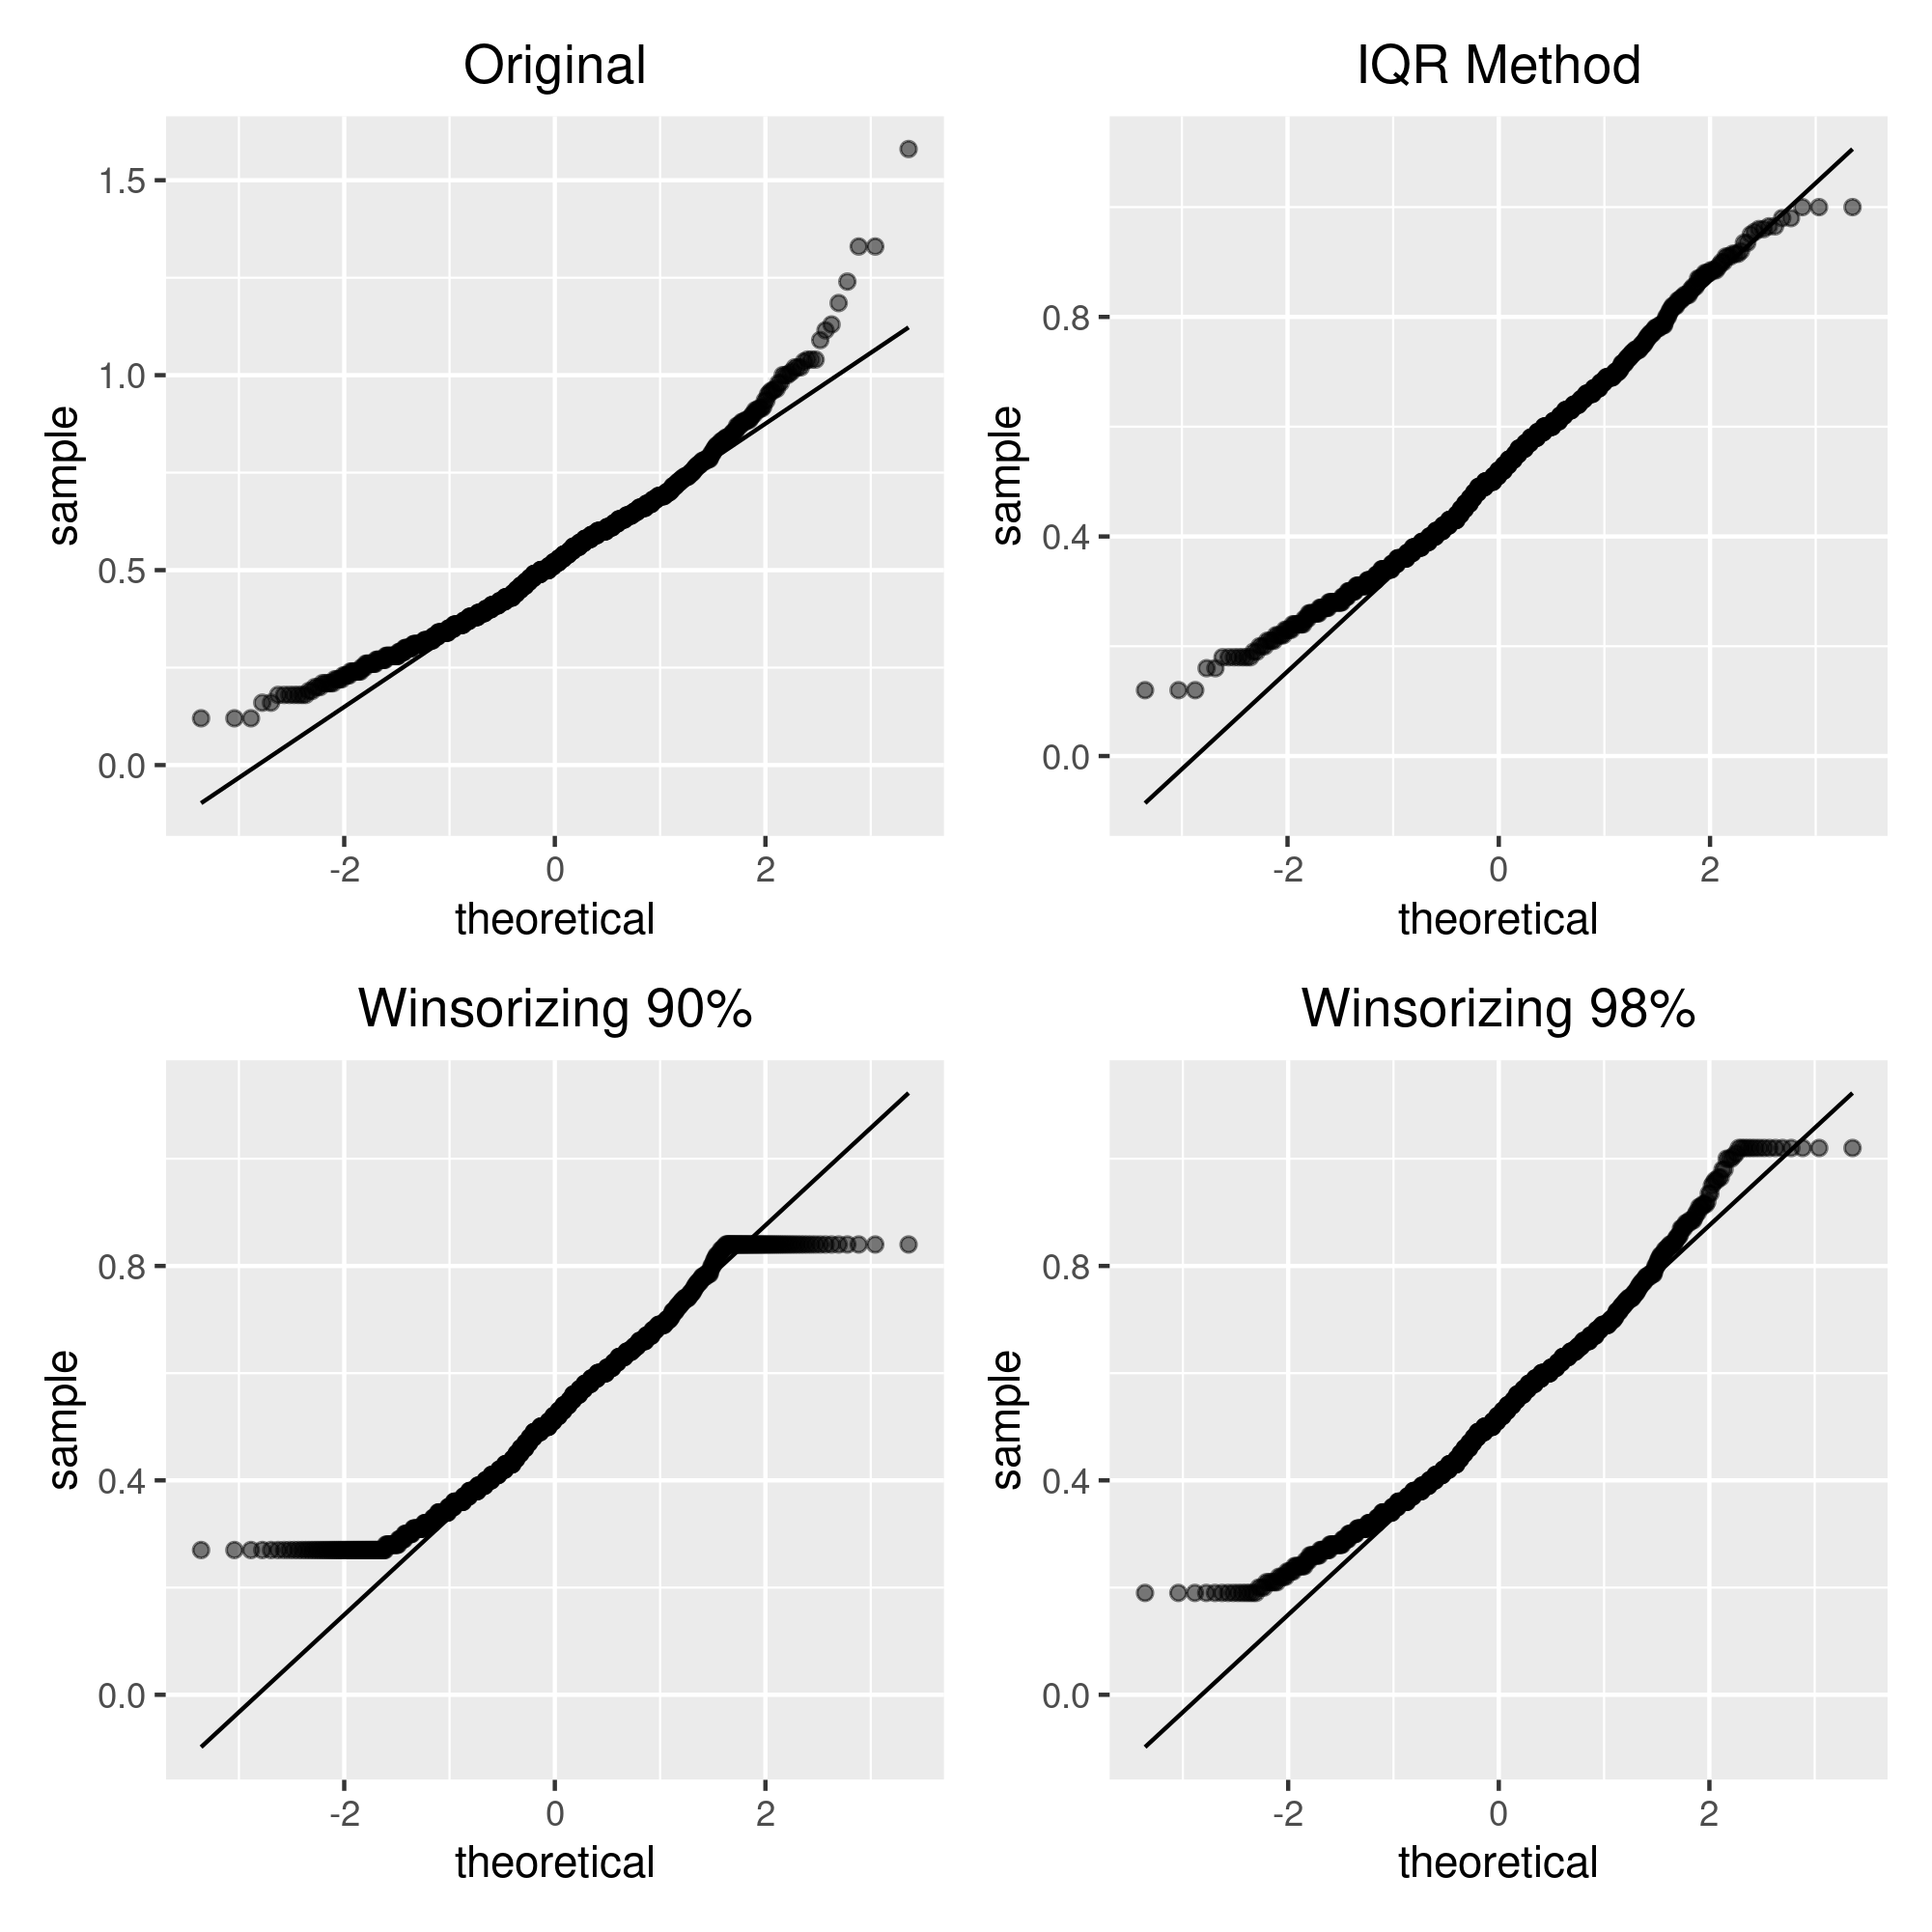
\includegraphics[width=0.45\textwidth]{images/outliers/volatile.acidity_qqplot.png}
    }

    \label{fig:volatile.acidity}
    \caption{Commento}
\end{figure}


\section{Correlazione}
In questo capitolo si analizza la relazione presente tra le diverse variabili tramite la matrice di correlazione.

\noindent
La matrice di correlazione mette in mostra la correlazione tra ogni coppia di variabili del dataset, per questo motivo otteniamo una matrice simmetrica.

\noindent
In questo caso abbiamo sull'anti-diagonale l'incrocio con la stessa identica variabile e questo comporta la correlazione massima.

\noindent
In seguito sono riportate le matrici di correlazione [\ref{fig:correlation_O}], [\ref{fig:correlation_NoO}] dove la seconda matrice mostra i dati dopo aver tolto gli outliers dal dataset .

\noindent
I valori positivi di correlazione indicano che all'aumentare dei valori di una variabile aumentano anche i valori assunti dall'altra variabile, mentre i valori di correlazione negativi indicano che al crescere dei valori di una variabile corrisponde un andamento di decrescita nei valori dell'altra variabile.

\noindent
Come si può notare otteniamo una correlazione molto bassa, questo conferma quanto precedentemente affermato riguardo alla difficoltà per un modello di poter inferire sui dati.

\noindent
Osservando i valori di correlazione che caratterizzano la variabile \textit{quality} si può notare come solo \textit{alcohol} e \textit{volatile.acidity} forniscono una correlazione utile per poter distinguere la classe di qualità, ma comunque con valori medio bassi e quindi poco significativi.

\noindent
Inoltre questa bassa correlazione suggerisce che l'utilizzo di una PCA non porterà a miglioramenti significativi.

\noindent
Come si può notare osservando i due grafici la rimozione degli outliers porta a piccoli miglioramenti aumentando la correlazione in valore assoluto.

\newpage

\begin{figure}[H]
    \centering
    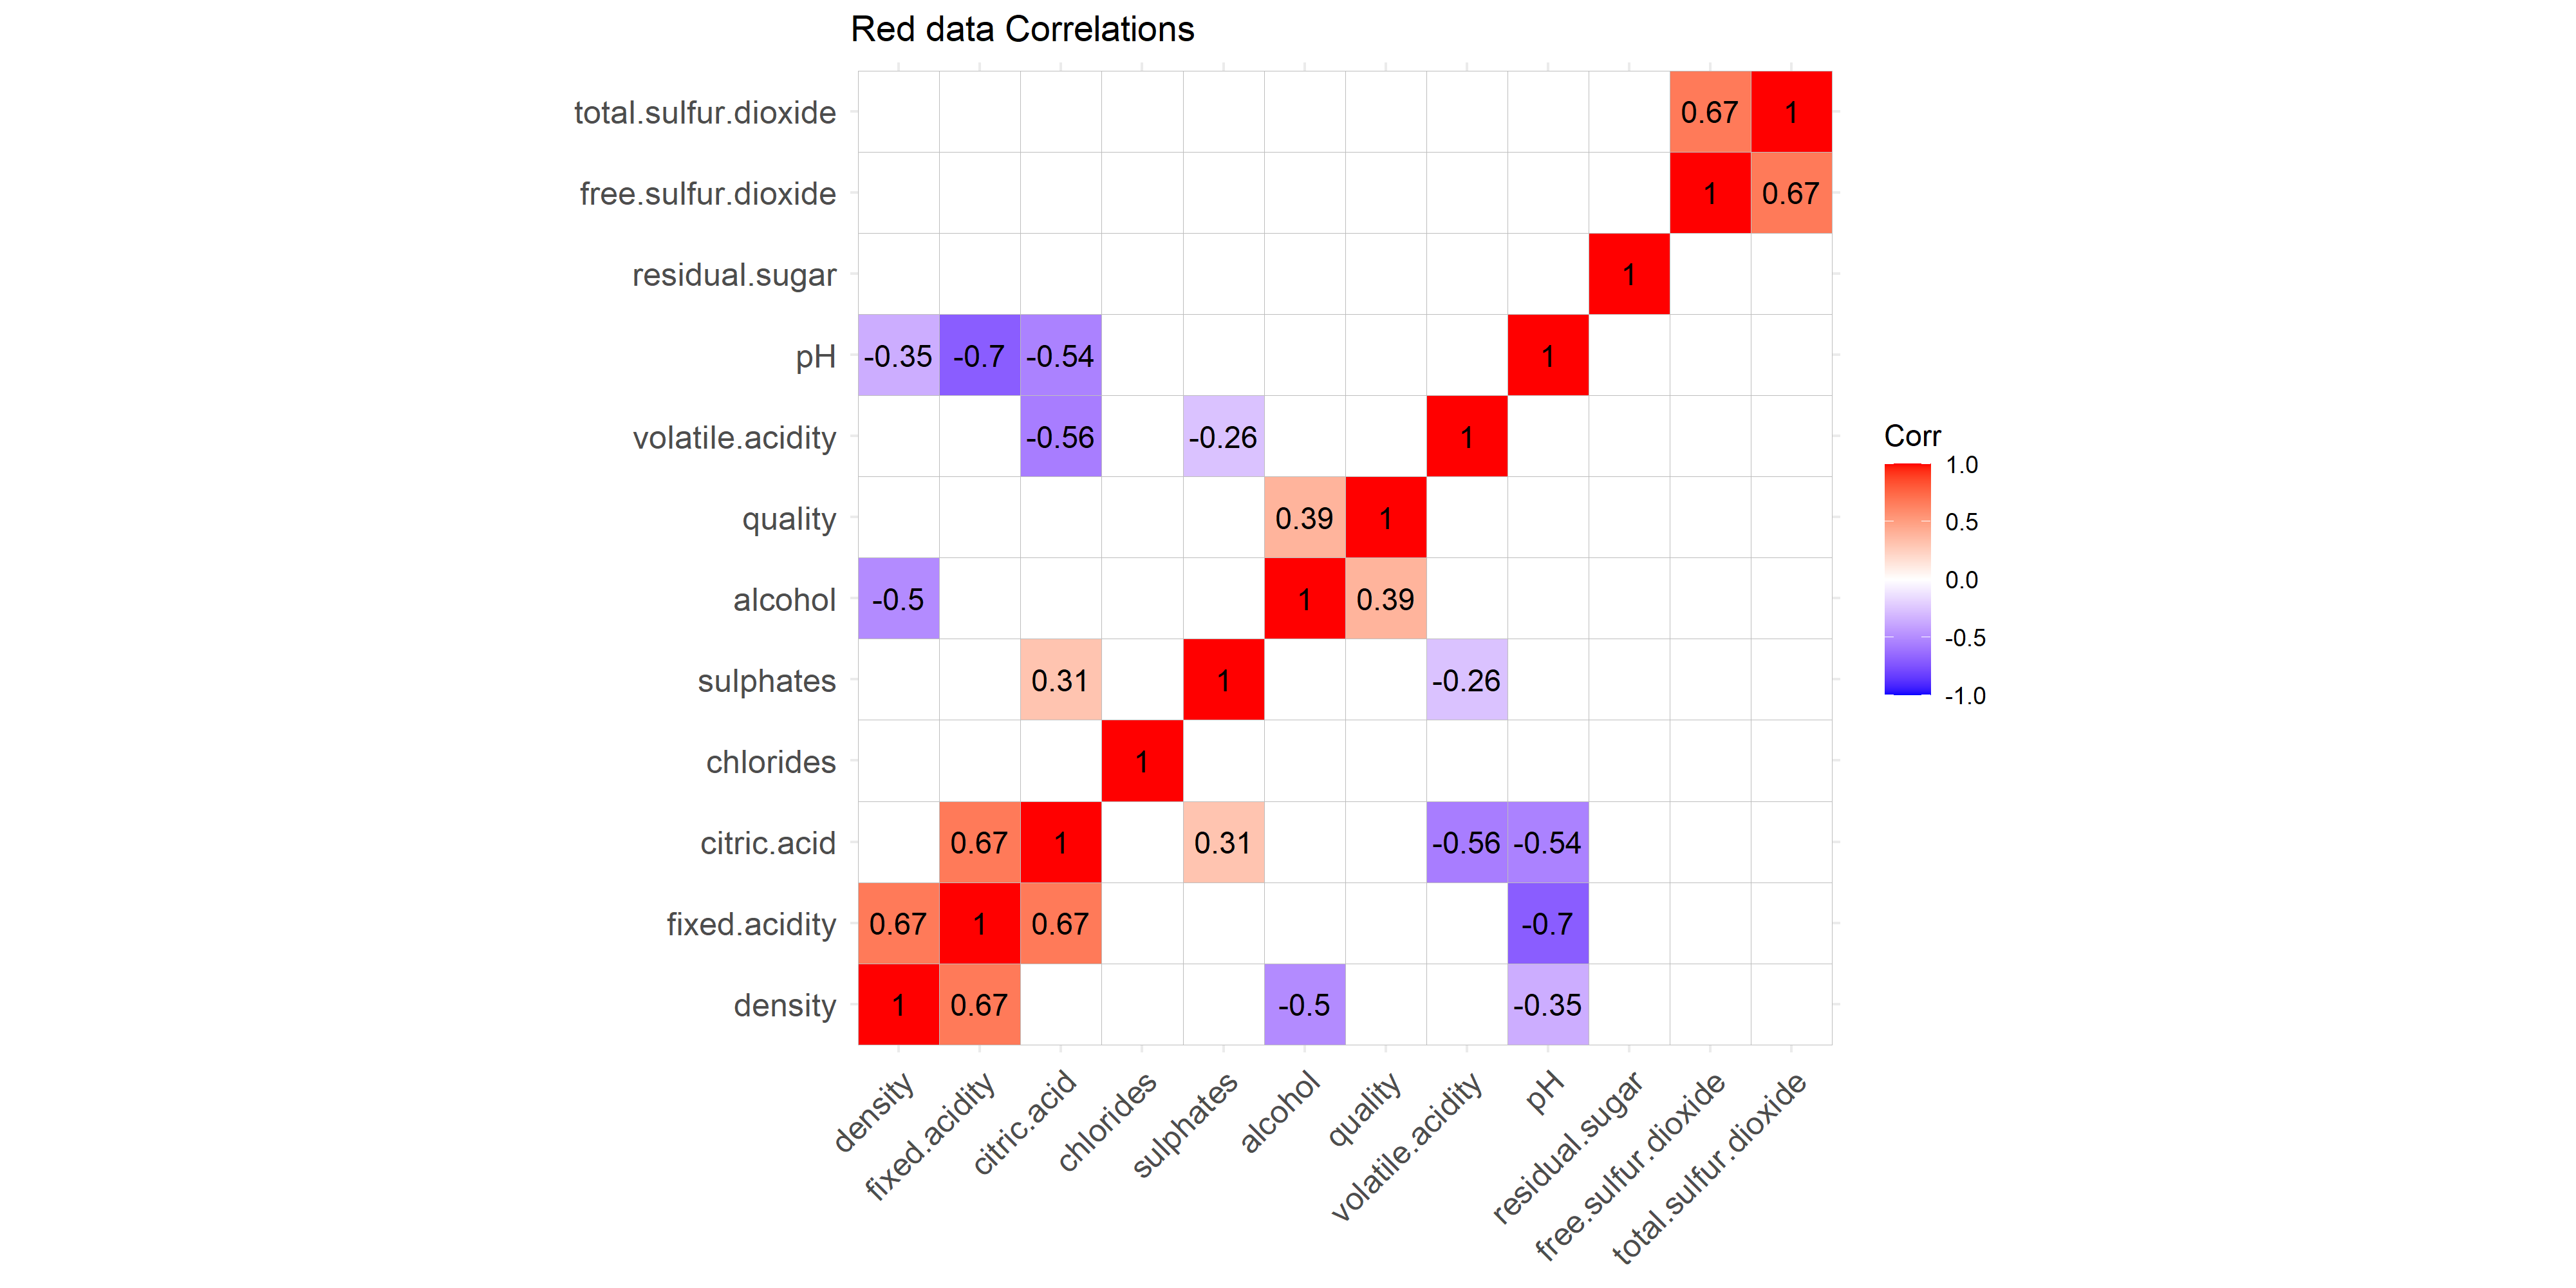
\includegraphics[scale=.5]{images/analisi/correlazione/Correlation_matrix_.pngO.png}
    \caption{Questa immagine rappresenta una matrice della correlazione che mette in evidenza le maggiori correlazioni tra le diverse variabili.}
    \label{fig:correlation_O}
\end{figure}

\begin{figure}[H]
    \centering
    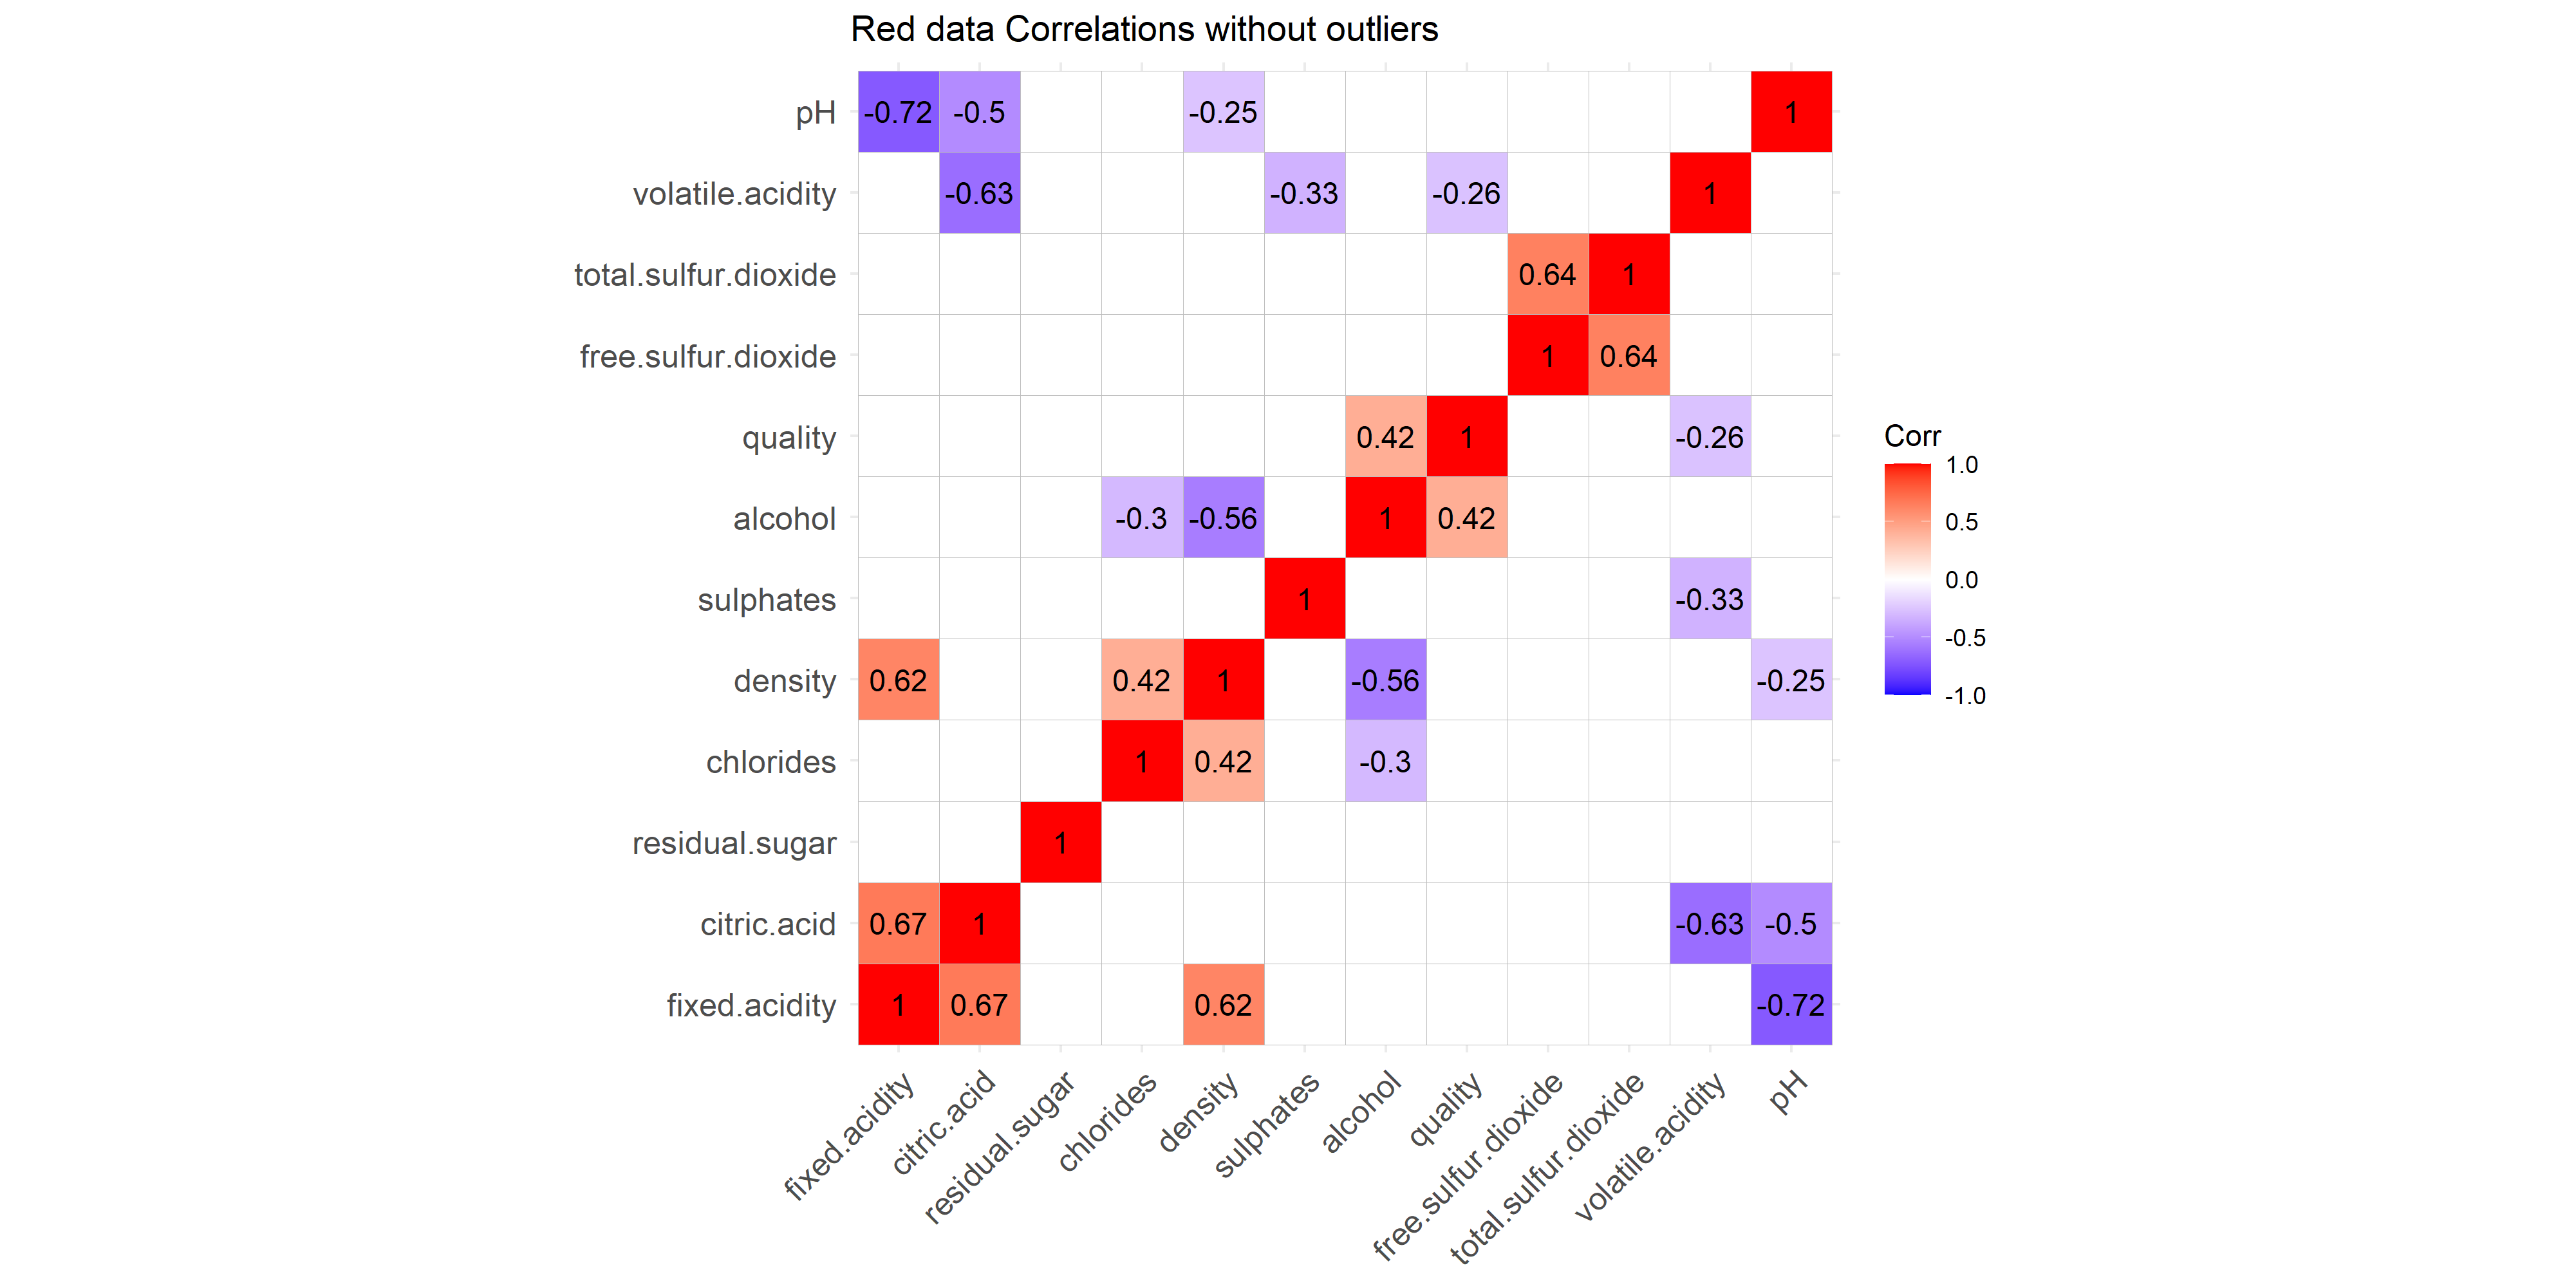
\includegraphics[scale=.5]{images/analisi/correlazione/Correlation_matrix_.pngNoO.png}
    \caption{Questa immagine rappresenta una matrice della correlazione che mette in evidenza le maggiori correlazioni tra le diverse variabili, in questo specifico caso il dataset non contiene gli outlier.}
    \label{fig:correlation_NoO}
\end{figure}


\section{Analisi delle componenti principali}
L'analisi delle componenti principali (in inglese principal component analysis o abbreviata PCA) è una tecnica di riduzione della dimensionalità di un insieme di dati utilizzata nell'ambito della statistica multivariata.

\noindent
Lo scopo della PCA è quello di ridurre il numero più o meno elevato di variabili che descrivono un insieme di dati a un numero minore di variabili, mantenendo le più importanti e limitando il più possibile la perdita di informazioni.

\noindent
Ciò avviene tramite una trasformazione lineare delle variabili che proietta quelle originarie in un nuovo sistema cartesiano \cite{PCA_wikipedia}.

\noindent
La riduzione della complessità avviene limitandosi ad analizzare le componenti principali, per varianza, tra le nuove variabili ottenute e scartando quelle con poca varianza.

\noindent
Nel nostro caso è stata applicata una \textit{feature extraction} ovvero sono state estratte le componenti principali dal dominio trasformato, invece la \textit{feature selection} seleziona un sottoinsieme delle variabili originali.

\noindent
La differenza principale è che la \textit{feature extraction} crea delle nuove variabili non presenti nel dominio originale.

\noindent
Nei grafici [\ref{fig:variance_O}] e [\ref{fig:variance_NoO}] che seguono è riportata un'analisi della varianza spiegata ovvero della varianza che ogni componente rappresenta rispetto alla varianza totale.

\noindent
Questo grafico permette di capire se la trasformazione può portare a dei benefici e mostra la varianza spiegata da ogni variabile.

\noindent
L'obiettivo è quello di prendere un numero ridotto di componenti cercando di rappresentare il 90-95\% della varianza spiegata.

\noindent
Come si può notare dai grafici per poter spiegare il 95\% sarebbe necessario prendere almeno 9 componenti rispetto alle 11 totali; questo mostra come la PCA porta miglioramenti non molto significativi.

\noindent
Anche rimuovendo gli outliers non si ottiene nessuna miglioria.

\newpage

\begin{figure}[H]
    \centering
    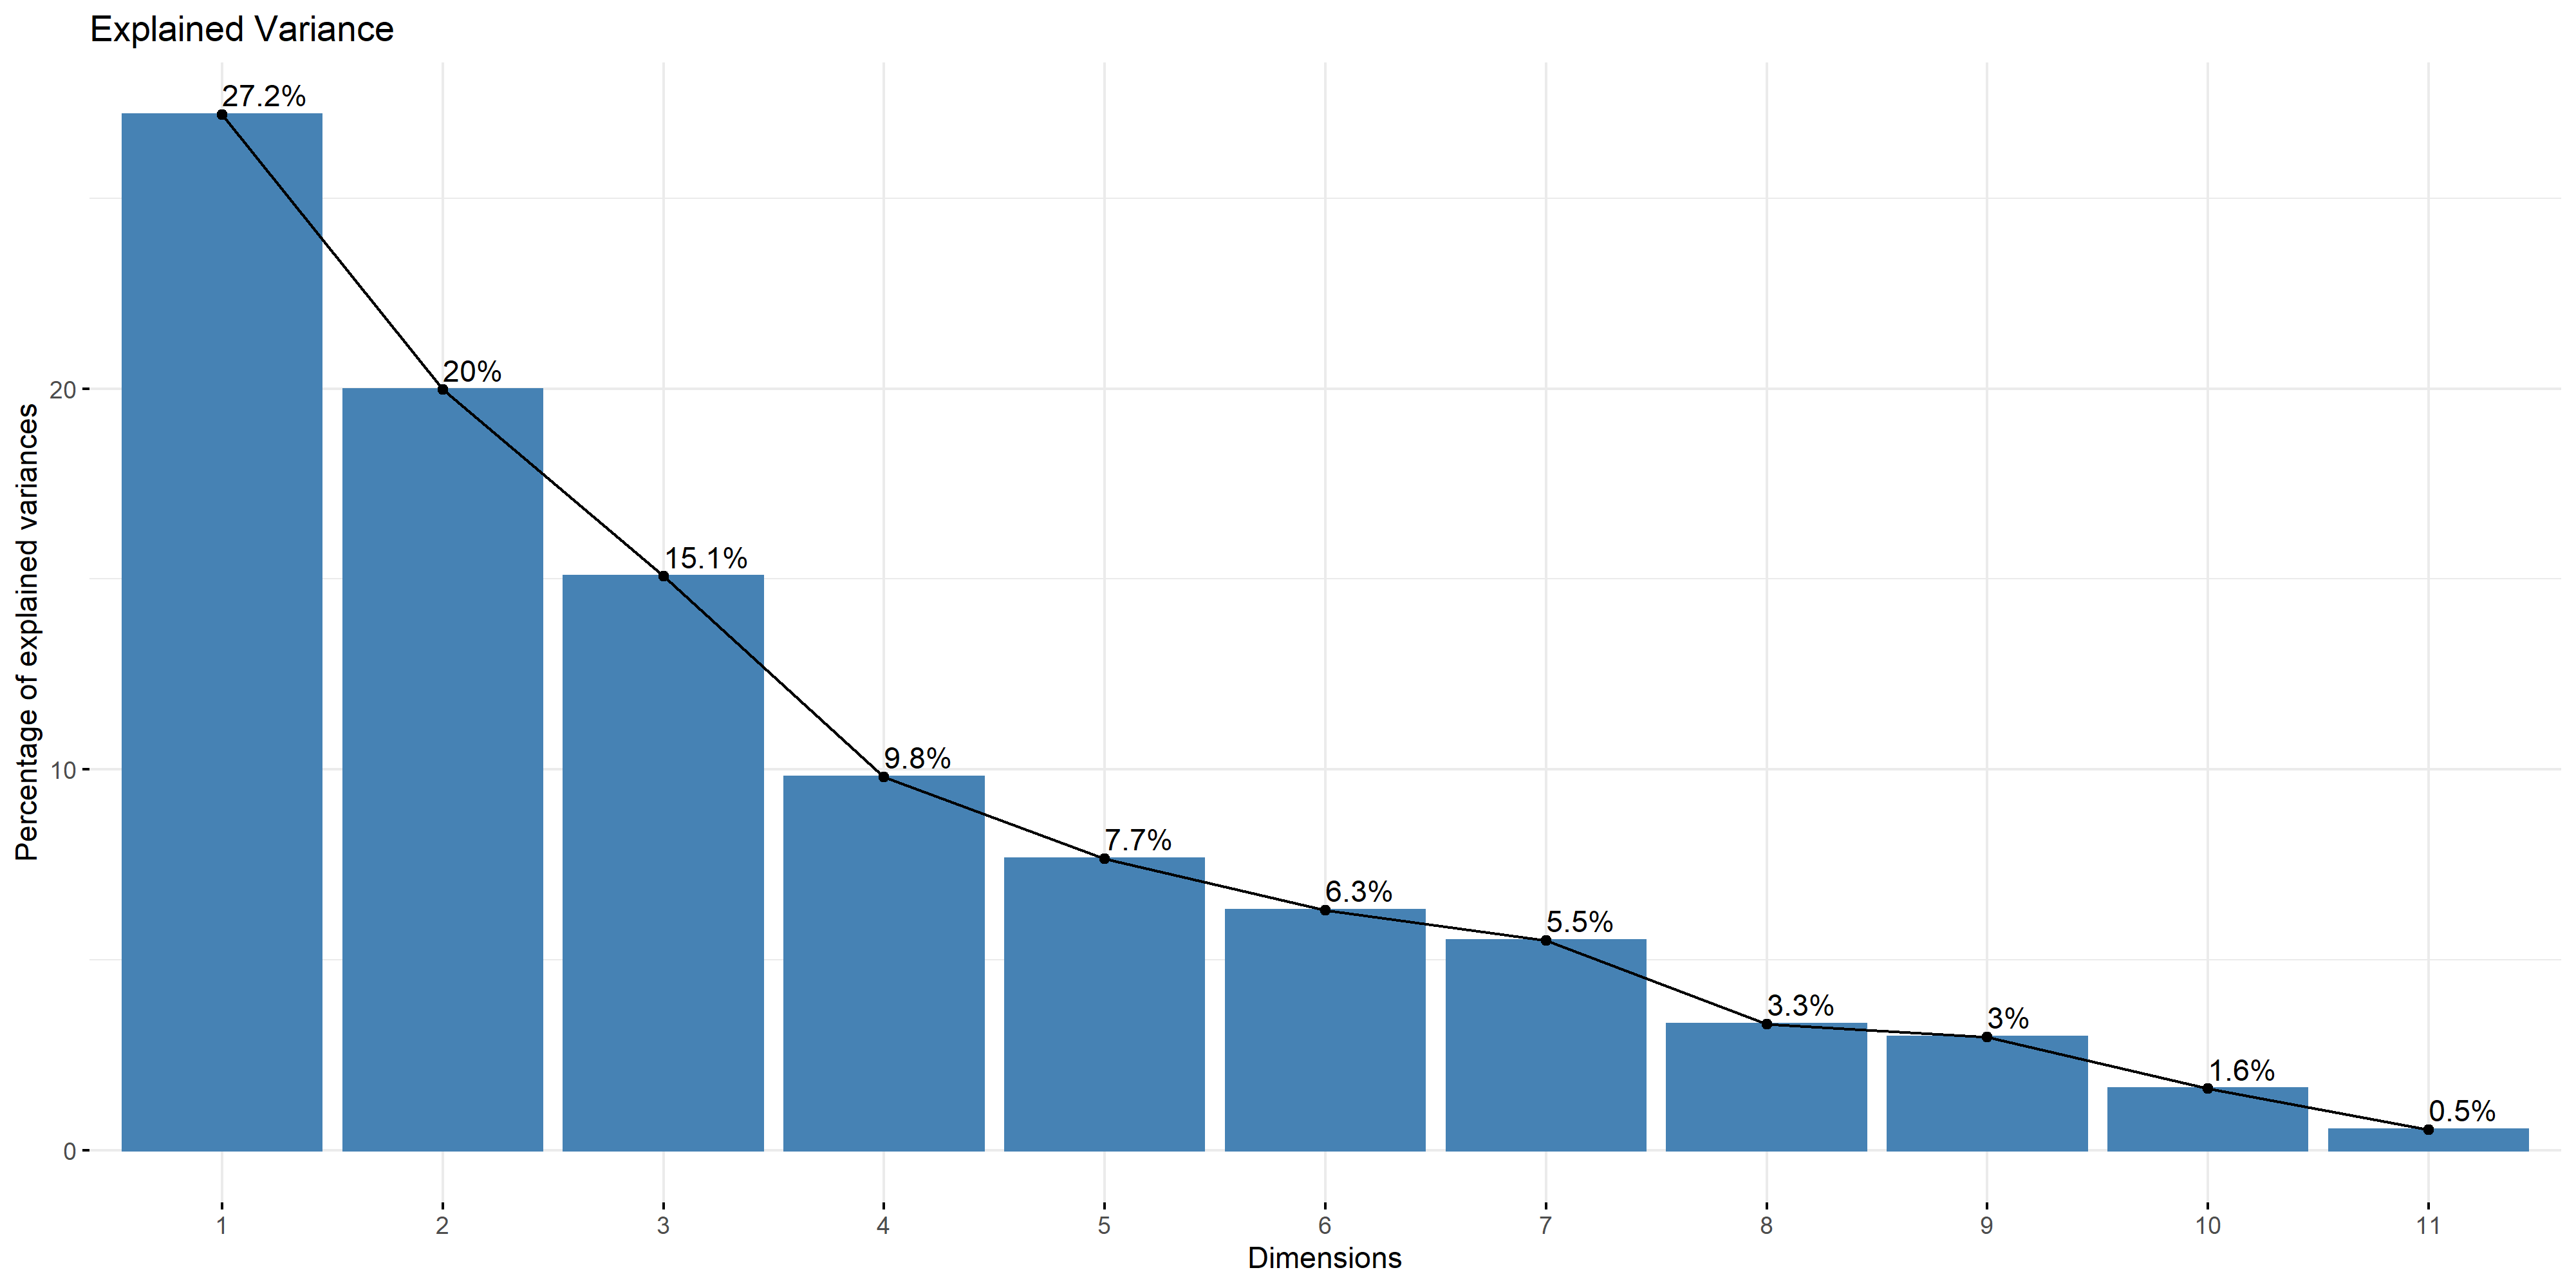
\includegraphics[scale=.4]{images/analisi/pca/variance_O.png}
    \caption{Questa immagine rappresenta la varianza spiegata per ogni componente della PCA.}
    \label{fig:variance_O}
\end{figure}

\begin{figure}[H]
    \centering
    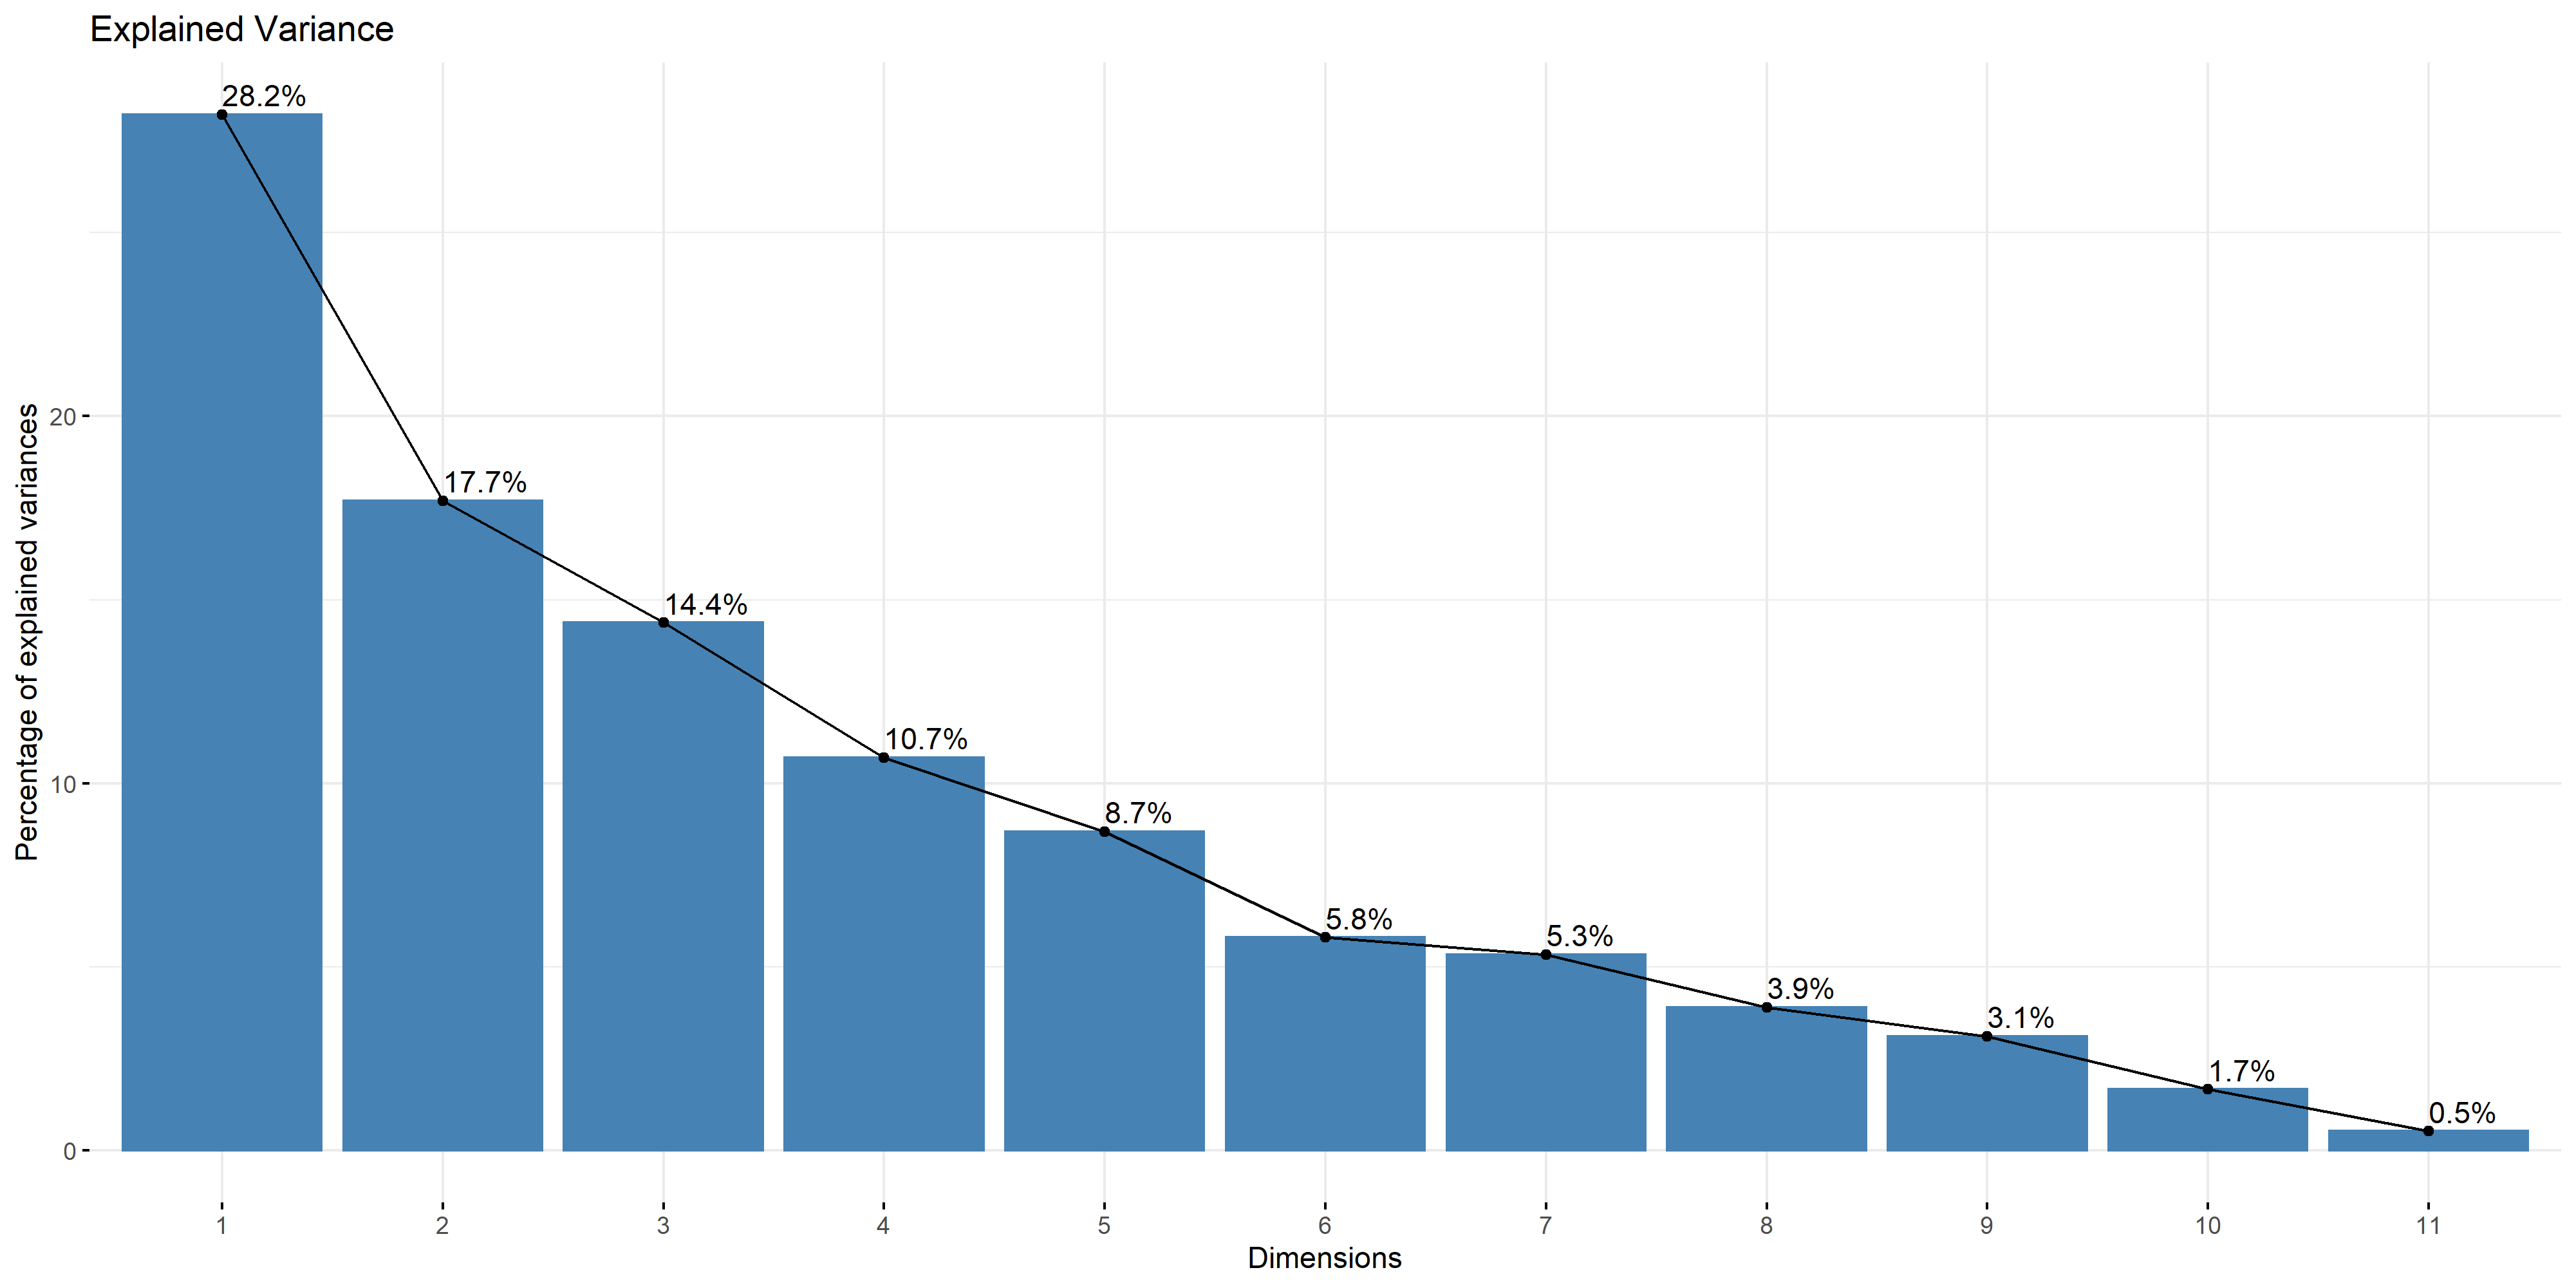
\includegraphics[scale=.4]{images/analisi/pca/variance_NoO.png}
    \caption{Questa immagine rappresenta la varianza spiegata per ogni componente della PCA; in questo caso dal dataset sono stati rimossi gli outliers.}
    \label{fig:variance_NoO}
\end{figure}
